\documentclass[11pt,a4paper,openany]{report}
% ============================================================
%  Préambule commun — Arbitrage Hub (Horacle Capital)
%  Police : Times (mathptmx), format article de recherche
% ============================================================
\usepackage[utf8]{inputenc}
\usepackage[T1]{fontenc}
\usepackage{mathptmx}            % Times New Roman (texte + maths)
\usepackage{courier}            % police à chasse fixe vectorielle
\usepackage{amsmath,amssymb,amsthm,bm}
\usepackage[a4paper,margin=2.4cm,headheight=14pt]{geometry}
\usepackage{microtype}
\usepackage{graphicx}
\usepackage{booktabs,tabularx,multirow,array,longtable}
\usepackage{enumitem}
\usepackage[dvipsnames,table]{xcolor}
\usepackage{fancyhdr}
\usepackage{titlesec}
\usepackage[font=small,labelfont=bf]{caption}
\usepackage[numbers,sort&compress]{natbib}
\usepackage{needspace}
\usepackage{tikz}
\usetikzlibrary{positioning,arrows.meta,fit,calc}
\usepackage{chngcntr}
\usepackage{listings}
\usepackage[most]{tcolorbox}
\usepackage{needspace}
\usepackage{abstract}
\usepackage[hidelinks,unicode]{hyperref}

\frenchspacing
\setlength{\parindent}{1.2em}
\setlength{\parskip}{0.35em}
\linespread{1.06}
\setlist{itemsep=0.15em,topsep=0.3em}
\hyphenpenalty=600
\emergencystretch=2em

% ---- Libellés en français (pas de babel-french sur la machine de build)
\renewcommand{\contentsname}{Table des matières}
\renewcommand{\refname}{Références}
\renewcommand{\bibname}{Bibliographie}
\renewcommand{\chaptername}{Chapitre}
\renewcommand{\partname}{Partie}
\renewcommand{\appendixname}{Annexe}
\renewcommand{\abstractname}{Résumé}
\renewcommand{\figurename}{Figure}
\renewcommand{\tablename}{Tableau}
\renewcommand{\listfigurename}{Liste des figures}
\newcommand{\og}{\guillemotleft\,}
\newcommand{\fg}{\,\guillemotright}

% ---- Titres de sections
\titleformat{\chapter}[display]{\normalfont\bfseries}{\large\scshape Chapitre \thechapter}{0.4em}{\LARGE}[\vspace{0.3em}\titlerule]
\titlespacing*{\chapter}{0pt}{-10pt}{18pt}
\titleformat{\part}[display]{\normalfont\centering\bfseries}{\Large\scshape Partie \thepart}{1em}{\Huge}
\titleformat{\section}{\normalfont\large\bfseries}{\thesection}{0.6em}{}
\titleformat{\subsection}{\normalfont\normalsize\bfseries}{\thesubsection}{0.5em}{}
\titleformat{\subsubsection}{\normalfont\normalsize\itshape}{\thesubsubsection.}{0.5em}{}

% ---- En-têtes
\pagestyle{fancy}
\fancyhf{}
\renewcommand{\headrulewidth}{0.4pt}
\fancyfoot[C]{\small\thepage}
\fancyhead[L]{\small\itshape Arbitrage Hub — cours complet}
\fancyhead[R]{\small\itshape\nouppercase{\leftmark}}
\renewcommand{\chaptermark}[1]{\markboth{Chapitre \thechapter{} — #1}{}}
\fancypagestyle{plain}{\fancyhf{}\renewcommand{\headrulewidth}{0pt}\fancyfoot[C]{\small\thepage}}

% ---- Théorèmes
\theoremstyle{definition}
\newtheorem{definition}{Définition}[chapter]
\newtheorem{example}{Exemple}[chapter]
\newtheorem{exercise}{Exercice}[chapter]
\theoremstyle{plain}
\newtheorem{proposition}{Proposition}[chapter]
\newtheorem{theorem}{Théorème}[chapter]
\newtheorem{lemma}{Lemme}[chapter]
\theoremstyle{remark}
\newtheorem{remark}{Remarque}[chapter]
\renewcommand{\proofname}{Démonstration}

% ---- Encadrés pédagogiques
\tcbset{boxrule=0.5pt,arc=1pt,left=6pt,right=6pt,top=4pt,bottom=4pt,fonttitle=\bfseries\small}
\newtcolorbox{intuition}[1][]{colback=Blue!3,colframe=Blue!55!black,title={Image mentale#1}}
\newtcolorbox{whiteboard}[1][]{colback=Goldenrod!6,colframe=Goldenrod!70!black,title={Au tableau blanc#1}}
\newtcolorbox{pitfall}[1][]{colback=Red!3,colframe=Red!60!black,title={Piège / limite#1}}
\newtcolorbox{toread}[1][]{colback=Gray!5,colframe=Gray!70!black,title={Pour aller plus loin — quoi lire#1}}
\newtcolorbox{codebox}[1][]{colback=Green!3,colframe=Green!45!black,title={Vérification en Python#1}}

% ---- Code
\lstset{basicstyle=\ttfamily\footnotesize,breaklines=true,columns=fullflexible,
  keywordstyle=\color{Blue!70!black},commentstyle=\color{Gray},stringstyle=\color{Maroon},
  frame=single,rulecolor=\color{Gray!40},xleftmargin=0.5em,xrightmargin=0.5em,
  literate={é}{{\'e}}1 {è}{{\`e}}1 {à}{{\`a}}1 {ç}{{\c c}}1 {ê}{{\^e}}1 {ô}{{\^o}}1 {î}{{\^i}}1 {ù}{{\`u}}1 {É}{{\'E}}1 {—}{{---}}1 {→}{{$\to$}}1}

% ---- Notations
\newcommand{\E}{\mathbb{E}}
\newcommand{\Var}{\operatorname{Var}}
\newcommand{\Cov}{\operatorname{Cov}}
\newcommand{\Corr}{\operatorname{Corr}}
\newcommand{\R}{\mathbb{R}}
\newcommand{\Prob}{\mathbb{P}}
\newcommand{\iid}{\overset{\text{i.i.d.}}{\sim}}
\newcommand{\N}{\mathcal{N}}
\newcommand{\dd}{\mathrm{d}}

\graphicspath{{figures/}}
\setcounter{tocdepth}{1}

\begin{document}

% =====================================================================
%  Page de titre
% =====================================================================
\begin{titlepage}
\centering
\vspace*{3cm}
{\Large\scshape Arbitrage Hub — Horacle Capital\par}
\vspace{1.2cm}
{\huge\bfseries Arbitrage statistique,\\[0.3em] pairs trading et arbitrage inter-plateformes\par}
\vspace{0.8cm}
{\Large Cours complet : de la théorie aux stratégies codées et auditées\par}
\vspace{2cm}
{\large Claude Opus 5.5 (Anthropic)\par}
\vspace{0.3cm}
{\normalsize Rédigé pour Léo Lombardini — Horacle Capital\par}
\vspace{0.2cm}
{\small\url{https://github.com/OptiWealthSolutions/arbitrage_hub}\par}
\vfill
{\large 20 octobre 2026\par}
\end{titlepage}

% =====================================================================
\pagenumbering{roman}
\chapter*{Résumé}
\addcontentsline{toc}{chapter}{Résumé}
\markboth{Résumé}{}
\noindent Ce document réunit en un seul volume un cours complet sur l'arbitrage statistique, le \emph{pairs trading} et l'arbitrage inter-plateformes accessible à un trader particulier. Il est organisé en un chapitre introductif et quatre parties.

\medskip\noindent\textbf{Chapitre 0} définit ce que recouvre le mot \og arbitrage\fg, fixe la méthode de travail, dresse la revue de littérature et analyse le moteur open source \texttt{atjte} d'arbitrage multi-plateformes.

\medskip\noindent\textbf{Partie I — Fondations statistiques (chapitres 1 à 5).} Arbitrage pur et statistique, stationnarité, marche aléatoire et AR(1) ; régression, maximum de vraisemblance et leurs biais ; tests de racine unitaire et de stationnarité ; cointégration d'Engle-Granger et de Johansen ; processus d'Ornstein-Uhlenbeck, temps de premier passage et seuils de trading optimaux.

\medskip\noindent\textbf{Partie II — Les méthodes de pairs trading (chapitres 6 à 11).} Méthode des distances de Gatev, Goetzmann et Rouwenhorst ; sélection de paires par cointégration et contrôle des faux positifs ; ratio de couverture dynamique par filtre de Kalman ; copules ; arbitrage statistique multi-actifs par analyse en composantes principales (Avellaneda et Lee) ; apprentissage automatique et validation sans fuite d'information.

\medskip\noindent\textbf{Partie III — Arbitrage inter-plateformes (chapitres 12 à 15).} Microstructure et modèle de coûts ; arbitrage spatial et triangulaire et course à la latence ; arbitrage de base, \emph{cash-and-carry} et \emph{funding} des contrats perpétuels, avec l'étude du cas \texttt{atjte} ; exécution, risque de jambe, sélection adverse et architecture logicielle.

\medskip\noindent\textbf{Partie IV — Validation, risque et mise en production (chapitres 16 à 18).} \emph{Backtest} sans biais, tests multiples, ratio de Sharpe déflaté et probabilité de surapprentissage ; dimensionnement, détection de rupture, limites de l'arbitrage ; passage du papier au code avec Claude Code, du cahier des charges au \emph{paper trading}.

\medskip\noindent Chaque affirmation quantitative importante est vérifiée par un script Python du dépôt \texttt{arbitrage\_hub}, sur données simulées (où la vérité est connue) ou sur des données réelles (GLD, GLDM, KO, PEP, 500 séances téléchargées via Interactive Brokers). Les résultats chiffrés reportés dans le texte sont ceux que produisent ces scripts. Le cours est honnête sur un point central : la littérature montre que les profits du \emph{pairs trading} classique ont fortement diminué depuis les années 2000 et que l'arbitrage \og pur\fg{} entre plateformes est une course de vitesse perdue d'avance pour un particulier. L'objectif est de construire un avantage réel, mesuré et robuste, pas de promettre un profit.

\medskip\noindent\textbf{Mots-clés :} arbitrage statistique, pairs trading, cointégration, Ornstein-Uhlenbeck, filtre de Kalman, copules, analyse en composantes principales, microstructure, arbitrage de base, \emph{funding}, surapprentissage, ratio de Sharpe déflaté.


\tableofcontents

\cleardoublepage
\pagenumbering{arabic}

% =====================================================================
\setcounter{chapter}{-1}
% =====================================================================
\chapter{Cartographie de l'arbitrage, méthode et revue de littérature}
\label{ch:0}
% =====================================================================


% =====================================================================
\section{Introduction : pourquoi ajouter l'arbitrage à un portefeuille de stratégies}
% =====================================================================

Un portefeuille de stratégies comprenant déjà une stratégie macro/quantitative et des \emph{Expert Advisors} (EA) déployés sur des comptes de \emph{prop firms} est, par construction, exposé à la direction des marchés. Même un EA qui alterne achats et ventes gagne de l'argent parce qu'il anticipe correctement un mouvement de prix. L'arbitrage statistique repose sur une logique différente : on ne parie pas sur le niveau d'un prix, mais sur la \emph{relation} entre plusieurs prix. On achète ce qui est relativement bon marché et on vend ce qui est relativement cher, de sorte que le mouvement général du marché s'annule en grande partie dans la position.

\begin{intuition}
Imaginez deux bateaux amarrés côte à côte dans un port agité. Prédire la hauteur d'un bateau dans une heure est presque impossible : elle dépend de la marée et des vagues. En revanche, l'écart de hauteur entre les deux bateaux reste petit, car ils sont soulevés par la même eau. L'arbitrage statistique consiste à parier sur cet \emph{écart}, pas sur la marée. Quand l'écart devient anormalement grand (une vague a frappé un bateau avant l'autre), on parie qu'il va se refermer.
\end{intuition}

Cette logique apporte une diversification réelle : un portefeuille \og neutre au marché\fg{} a, en principe, une faible corrélation avec des stratégies directionnelles. Mais elle comporte des risques propres, très différents : la relation entre les prix peut se rompre définitivement, les coûts de transaction peuvent dévorer un avantage de quelques points de base, et l'exécution simultanée de deux ordres sur deux plateformes peut échouer à moitié. Ce cours étudie ces trois questions avec autant de soin que la théorie.

\subsection{Objectifs d'apprentissage}

À la fin du cours, vous devez être capable de :
\begin{enumerate}[label=\textbf{O\arabic*.}]
\item distinguer formellement arbitrage pur, quasi-arbitrage de convergence et arbitrage statistique, et dire pour chaque opportunité dans quelle catégorie elle tombe ;
\item démontrer les propriétés des processus utilisés (marche aléatoire, AR(1), processus d'Ornstein-Uhlenbeck, systèmes cointégrés) et savoir les estimer sur données réelles ;
\item appliquer et interpréter les tests statistiques (ADF, KPSS, Engle-Granger, Johansen, ratio de variance, exposant de Hurst) en connaissant leurs hypothèses et leurs faiblesses ;
\item implémenter les cinq grandes familles de \emph{pairs trading} (distance, cointégration, séries temporelles, copules, apprentissage automatique) ainsi que l'arbitrage multi-facteurs ;
\item modéliser une opportunité inter-plateformes (arbitrage spatial, triangulaire, de base, de \emph{funding}) en intégrant frais, latence, financement et risque de contrepartie ;
\item valider une stratégie sans se mentir : séparation formation/test, coûts réalistes, tests multiples, ratio de Sharpe déflaté, probabilité de surapprentissage ;
\item rédiger un cahier des charges que Claude Code peut transformer en code testé, puis déployer progressivement (papier, petite taille, taille cible).
\end{enumerate}

\subsection{Ce que ce cours ne promet pas}

Le but final est de générer du profit, et c'est légitime. Mais la littérature impose trois constats que nous garderons en tête à chaque chapitre. Premièrement, la rentabilité du \emph{pairs trading} simple sur actions américaines a nettement baissé au fil du temps \citep{dofaff2010,dofaff2012}. Deuxièmement, l'arbitrage pur entre plateformes est une course de vitesse que les acteurs institutionnels gagnent à la milliseconde \citep{budish2015}. Troisièmement, la plupart des stratégies qui semblent rentables en \emph{backtest} le sont par hasard, parce qu'on a essayé beaucoup de variantes \citep{bailey2014dsr,harvey2016}. Le cours est construit pour transformer ces trois obstacles en critères de sélection.

% =====================================================================
\section{Méthode de travail}
% =====================================================================

\subsection{Un chapitre à la fois}
Le cours est réuni dans ce seul document, mais il se travaille chapitre par chapitre : on ne passe au suivant que lorsque les exercices du précédent sont faits et que les scripts Python associés tournent sur votre machine. Chaque chapitre suit la même structure :
\begin{enumerate}
\item \textbf{Intuition} : une image mentale (encadré bleu) avant toute formule ;
\item \textbf{Formalisation} : définitions, propositions et démonstrations, chaque étape algébrique justifiée ;
\item \textbf{Vérification} : un script Python teste l'hypothèse au lieu de l'affirmer (encadré vert) ;
\item \textbf{Limites} : ce que la théorie ne dit pas, et comment cela peut coûter de l'argent (encadré rouge) ;
\item \textbf{Fiche tableau blanc} : les formules à recopier et annoter (encadré jaune) ;
\item \textbf{Quoi lire} : références précises (article, section ou chapitre) pour approfondir (encadré gris) ;
\item \textbf{Exercices}, dont au moins un à coder.
\end{enumerate}

\subsection{Le tableau blanc}
Le tableau blanc sert à \emph{reconstruire} les démonstrations, pas à les recopier. La méthode conseillée : (1) lire la section une fois sans écrire ; (2) fermer le PDF et réécrire au tableau la définition et l'énoncé ; (3) refaire la démonstration en ne rouvrant le PDF qu'en cas de blocage ; (4) photographier le tableau et déposer la photo dans \texttt{whiteboard/chXX/} du dépôt, pour garder une trace datée de votre progression.

\subsection{Le cycle \og hypothèse $\rightarrow$ script $\rightarrow$ conclusion\fg}
Aucune affirmation importante du cours ne doit être crue sur parole. Chaque fois qu'une propriété est énoncée (par exemple \og la variance d'une marche aléatoire croît linéairement avec le temps\fg), un script dans \texttt{code/chXX/} la vérifie par simulation ou sur données réelles, et le résultat chiffré figure dans le chapitre. Vous pouvez relancer chaque script et obtenir les mêmes nombres (graines aléatoires fixées).


\subsection{Données réelles et données simulées}
Deux sortes d'expériences coexistent dans le cours. Les \textbf{simulations} placent la stratégie dans un monde dont on connaît la vérité (le vrai $\beta$, la vraie demi-vie) : c'est le seul moyen de vérifier qu'une méthode retrouve ce qu'elle prétend mesurer. Les \textbf{études de cas réelles} utilisent les clôtures quotidiennes de quatre titres téléchargées via l'API d'Interactive Brokers le 20 octobre 2026 (500 séances, du 21 octobre 2024 au 19 octobre 2026) : deux ETF adossés à l'or physique, GLD et GLDM, qui forment un quasi-arbitrage, et deux actions du même secteur, Coca-Cola (KO) et PepsiCo (PEP), qui forment la paire statistique la plus citée des manuels. Les fichiers sont dans \texttt{data/case\_studies/}. Deux ans de données, c'est court : les études de cas illustrent les méthodes, elles ne prétendent pas établir la rentabilité d'une stratégie.

\subsection{Comment lire les encadrés}
\begin{itemize}
\item \textbf{Image mentale} (bleu) : l'intuition, à comprendre avant la formule.
\item \textbf{Au tableau blanc} (jaune) : les formules à reconstruire et annoter.
\item \textbf{Piège / limite} (rouge) : ce qui peut coûter de l'argent.
\item \textbf{Vérification en Python} (vert) : une hypothèse testée, avec le script et les chiffres obtenus.
\item \textbf{Pour aller plus loin} (gris) : quoi lire, avec la section ou le chapitre précis.
\end{itemize}

% =====================================================================
\section{Cartographie : que veut dire \og arbitrage\fg{} ?}\label{c0:carto}
% =====================================================================

Le mot \og arbitrage\fg{} est utilisé de façon très lâche sur les réseaux sociaux. Nous distinguerons trois familles, définies formellement au chapitre~1.

\begin{description}
\item[Arbitrage pur.] Une stratégie qui ne coûte rien aujourd'hui, ne peut jamais perdre, et gagne avec une probabilité strictement positive. Exemple : un même actif coté à deux prix différents au même instant, achetable et vendable simultanément. En pratique, l'arbitrage pur n'existe que pendant des fractions de seconde, ou en présence de frictions (frais, transferts, contrôles des capitaux) qui en font justement autre chose qu'un arbitrage pur.
\item[Quasi-arbitrage de convergence.] Deux instruments liés par une relation \emph{contractuelle} ou \emph{économique forte} (un contrat à terme et son sous-jacent, un jeton adossé à l'or et un CFD sur l'or, un ETF et son panier) dont l'écart doit converger à une date connue ou rester borné. Le risque existe (l'écart peut s'élargir avant de converger, le financement peut coûter cher), mais la relation a une \emph{ancre} théorique.
\item[Arbitrage statistique.] Une relation purement \emph{estimée} à partir de données historiques (deux actions du même secteur, un panier de devises) et supposée persister. Aucune loi n'oblige la relation à durer : c'est un pari à espérance positive, justifié par des tests statistiques, et c'est la famille la plus exposée au risque de rupture.
\end{description}

\begin{table}[h]
\centering\small
\caption{Taxonomie des stratégies étudiées dans le cours.}
\label{c0:tab:taxo}
\begin{tabularx}{\textwidth}{>{\raggedright}p{3.1cm}>{\raggedright}p{2.2cm}>{\raggedright}X>{\raggedright\arraybackslash}p{2.3cm}}
\toprule
Stratégie & Famille & Source de l'écart et ancre & Chapitres \\
\midrule
Arbitrage spatial (même actif, deux plateformes) & Pur / quasi & Fragmentation, frais, transferts lents \citep{makarov2020} & 12, 13 \\
Arbitrage triangulaire (FX, crypto) & Pur & Incohérence de trois taux croisés & 13 \\
Base \emph{cash-and-carry} (futures vs comptant) & Quasi & Coût de portage, convergence à l'échéance \citep{hull2022} & 14 \\
\emph{Funding} des perpétuels & Quasi & Taux de financement périodique & 14 \\
Perpétuel/jeton vs CFD (cas \texttt{atjte}) & Quasi & Même sous-jacent, deux plateformes \citep{atjte} & 14, 15 \\
\emph{Pairs trading} par distance & Statistique & Co-mouvement historique \citep{gatev2006} & 6 \\
\emph{Pairs trading} par cointégration & Statistique & Équilibre de long terme \citep{englegranger1987} & 4, 7 \\
Modèles espace-état, Kalman & Statistique & Ratio de couverture variable \citep{elliott2005} & 8 \\
Copules & Statistique & Dépendance non linéaire \citep{liewwu2013} & 9 \\
Multi-facteurs (ACP, résidus) & Statistique & Résidus d'un modèle de facteurs \citep{avellaneda2010} & 10 \\
Apprentissage automatique & Statistique & Prévision des résidus \citep{krauss2017ml} & 11 \\
\bottomrule
\end{tabularx}
\end{table}

% =====================================================================
\section{Prérequis mathématiques et statistiques}
% =====================================================================

Le tableau~\ref{c0:tab:prereq} liste les notions nécessaires, l'endroit où elles servent et le chapitre où elles sont (re)vues. Celles marquées $\star$ sont indispensables dès le chapitre~1 ; les autres sont introduites au moment où elles servent.

\begin{table}[h]
\centering\small
\caption{Prérequis et lieu d'utilisation.}
\label{c0:tab:prereq}
\begin{tabularx}{\textwidth}{>{\raggedright}p{4.3cm}>{\raggedright}X>{\raggedright\arraybackslash}p{1.6cm}}
\toprule
Notion & À quoi elle sert dans le cours & Chapitre \\
\midrule
$\star$ Espérance, variance, covariance, corrélation & Variance d'un \emph{spread}, ratio de couverture optimal & 1 \\
$\star$ Loi normale, quantiles & Seuils d'entrée en \emph{z-score}, intervalles de confiance & 1 \\
$\star$ Suites géométriques, logarithmes & Fonction d'autocorrélation, demi-vie & 1 \\
Régression linéaire, moindres carrés & Ratio de couverture, test d'Engle-Granger & 2 \\
Maximum de vraisemblance & Estimation AR(1) et Ornstein-Uhlenbeck & 2, 5 \\
Tests d'hypothèse, $p$-valeur, puissance & ADF, KPSS, tests multiples & 3, 16 \\
Algèbre linéaire (matrices, valeurs propres) & Johansen, ACP, portefeuilles multi-actifs & 4, 10 \\
Calcul stochastique de base (mouvement brownien, lemme d'Itô) & Processus d'Ornstein-Uhlenbeck & 5 \\
Temps d'arrêt, temps de premier passage & Seuils optimaux \citep{bertram2010,leungli2015} & 5 \\
Modèles espace-état, filtrage bayésien & Filtre de Kalman & 8 \\
Copules, théorème de Sklar & Dépendance non gaussienne & 9 \\
Apprentissage supervisé, validation croisée purgée & Sélection de paires, prévision & 11, 16 \\
Microstructure (carnet d'ordres, \emph{maker}/\emph{taker}) & Coûts réels, exécution inter-plateformes & 12, 15 \\
Évaluation des futures (portage) & Arbitrage de base et de \emph{funding} & 14 \\
\bottomrule
\end{tabularx}
\end{table}

% =====================================================================
\section{Programme détaillé}
% =====================================================================

La figure~\ref{c0:fig:map} donne l'ordre des dépendances. Les flèches indiquent \og doit être compris avant\fg.

\begin{figure}[h]
\centering
\begin{tikzpicture}[node distance=0.45cm and 0.5cm,
  box/.style={draw,rounded corners=2pt,font=\scriptsize,align=center,minimum width=2.3cm,minimum height=0.75cm,fill=white},
  arr/.style={-{Stealth[length=4pt]},thin,gray!70!black}]
\node[box,fill=Blue!8] (c1) {Ch.~1\\Fondations};
\node[box,fill=Blue!8,right=of c1] (c2) {Ch.~2\\Régression, MV};
\node[box,fill=Blue!8,right=of c2] (c3) {Ch.~3\\Tests de\\stationnarité};
\node[box,fill=Blue!8,right=of c3] (c4) {Ch.~4\\Cointégration};
\node[box,fill=Blue!8,right=of c4] (c5) {Ch.~5\\Ornstein-\\Uhlenbeck};
\node[box,fill=Green!8,below=0.9cm of c1] (c6) {Ch.~6\\Distance};
\node[box,fill=Green!8,right=of c6] (c7) {Ch.~7\\Cointégration\\appliquée};
\node[box,fill=Green!8,right=of c7] (c8) {Ch.~8\\Kalman};
\node[box,fill=Green!8,right=of c8] (c9) {Ch.~9\\Copules};
\node[box,fill=Green!8,right=of c9] (c10) {Ch.~10\\Multi-facteurs};
\node[box,fill=Green!8,below=0.9cm of c10] (c11) {Ch.~11\\Machine\\learning};
\node[box,fill=Orange!10,below=0.9cm of c6] (c12) {Ch.~12\\Microstructure};
\node[box,fill=Orange!10,right=of c12] (c13) {Ch.~13\\Spatial et\\triangulaire};
\node[box,fill=Orange!10,right=of c13] (c14) {Ch.~14\\Base et\\\emph{funding}};
\node[box,fill=Orange!10,right=of c14] (c15) {Ch.~15\\Exécution\\et couverture};
\node[box,fill=Red!8,below=0.9cm of c12] (c16) {Ch.~16\\Backtest\\rigoureux};
\node[box,fill=Red!8,right=of c16] (c17) {Ch.~17\\Risque et\\limites};
\node[box,fill=Red!8,right=of c17] (c18) {Ch.~18\\Du papier\\au code};
\draw[arr] (c1)--(c2); \draw[arr] (c2)--(c3); \draw[arr] (c3)--(c4); \draw[arr] (c4)--(c5);
\draw[arr] (c1)--(c6); \draw[arr] (c4)--(c7); \draw[arr] (c7)--(c8); \draw[arr] (c8)--(c9); \draw[arr] (c9)--(c10); \draw[arr] (c10)--(c11);
\draw[arr] (c5)--(c10);
\draw[arr] (c6)--(c12); \draw[arr] (c12)--(c13); \draw[arr] (c13)--(c14); \draw[arr] (c14)--(c15);
\draw[arr] (c12)--(c16); \draw[arr] (c16)--(c17); \draw[arr] (c17)--(c18); \draw[arr] (c15)--(c18); \draw[arr] (c11)--(c18);
\end{tikzpicture}
\caption{Carte du cours. Bleu : fondations ; vert : méthodes de \emph{pairs trading} ; orange : arbitrage inter-plateformes ; rouge : validation, risque et mise en production.}
\label{c0:fig:map}
\end{figure}

Pour chaque chapitre, nous indiquons les notions mathématiques, les lectures de référence et le code associé. Le code vit dans \texttt{code/chXX/} pendant l'apprentissage, puis les fonctions réutilisables migrent dans le paquet \texttt{src/arbhub/}.

\subsection{Partie I — Fondations statistiques}

\paragraph{Chapitre 1 — Arbitrage, stationnarité et retour à la moyenne.}
Définitions formelles de l'arbitrage pur et de l'arbitrage statistique \citep{hogan2004} ; rappels de probabilités (espérance, variance, covariance, variance d'une combinaison linéaire) ; ratio de couverture à variance minimale ; processus stochastiques, bruit blanc, stationnarité ; marche aléatoire ; processus AR(1), moyenne et variance stationnaires, autocorrélation, demi-vie ; intuition de la cointégration \citep{murray1994} ; corrélation contre cointégration ; \emph{z-score} et première règle de trading. \textbf{Code :} cinq scripts qui testent les propriétés énoncées. \textbf{Lire :} \citet{hamilton1994} ch.~3 ; \citet{chan2013} ch.~2.

\paragraph{Chapitre 2 — Régression et estimation.}
Moindres carrés ordinaires (dérivation matricielle), hypothèses de Gauss-Markov, propriétés des résidus ; régression fallacieuse \citep{granger1974} ; maximum de vraisemblance, application à l'AR(1) ; biais des petits échantillons sur le coefficient autorégressif ; régression orthogonale (moindres carrés totaux) et asymétrie du choix $Y$ sur $X$ contre $X$ sur $Y$. \textbf{Code :} estimateurs écrits à la main, comparés à \texttt{statsmodels} \citep{statsmodels}.

\paragraph{Chapitre 3 — Tester la stationnarité et le retour à la moyenne.}
Test de Dickey-Fuller et version augmentée \citep{dickeyfuller1979} : pourquoi la statistique ne suit pas une loi de Student ; test KPSS \citep{kpss1992} et logique d'hypothèse nulle inversée ; ratio de variance \citep{lomackinlay1988} ; exposant de Hurst ; puissance des tests sur échantillons courts ; tests multiples sur un univers de paires. \textbf{Code :} simulation de la distribution de Dickey-Fuller ; courbe de puissance en fonction de la taille d'échantillon.

\paragraph{Chapitre 4 — Cointégration.}
Ordre d'intégration, définition de la cointégration ; méthode en deux étapes d'Engle-Granger et valeurs critiques spécifiques \citep{englegranger1987} ; modèle à correction d'erreur ; théorème de représentation de Granger ; VAR, VECM et procédure de Johansen (tests de la trace et de la valeur propre maximale) \citep{johansen1991} ; cointégration partielle \citep{clegg2018}. \textbf{Code :} générateur de systèmes cointégrés ; implémentation pas à pas d'Engle-Granger ; comparaison avec Johansen.

\paragraph{Chapitre 5 — Le processus d'Ornstein-Uhlenbeck.}
Mouvement brownien, équation différentielle stochastique, lemme d'Itô ; solution explicite \citep{uhlenbeck1930} ; lien exact avec l'AR(1) ; estimation par maximum de vraisemblance ; temps de premier passage ; seuils d'entrée et de sortie optimaux \citep{bertram2010}, avec coûts et stop-loss \citep{leungli2015,leungli2016}. \textbf{Code :} simulation exacte, estimation, optimisation numérique des seuils.

\subsection{Partie II — Les méthodes de \emph{pairs trading}}

Cette partie suit la taxonomie de la revue de \citet{krauss2017survey}, qui classe la littérature en approches par distance, cointégration, séries temporelles, contrôle stochastique et \og autres\fg{} (copules, apprentissage).

\paragraph{Chapitre 6 — La méthode des distances.}
Réplication de \citet{gatev2006} : normalisation des prix, somme des écarts quadratiques, période de formation de douze mois, période de trading de six mois, seuil de deux écarts-types ; calcul des rendements sur capital engagé ; résultats de \citet{dofaff2010,dofaff2012} sur la baisse de rentabilité et l'effet des coûts. \textbf{Code :} réplication sur un univers d'actions ou d'ETF accessible via Interactive Brokers.

\paragraph{Chapitre 7 — Cointégration appliquée.}
Sélection des paires (secteur, cointégration, demi-vie, nombre de croisements de la moyenne) \citep{vidyamurthy2004,huck2009} ; ratio de couverture statique contre glissant ; comparaison distance/cointégration/copule \citep{rad2016} ; risque de rupture et suivi en ligne. \textbf{Code :} pipeline de sélection avec correction pour tests multiples.

\paragraph{Chapitre 8 — Modèles espace-état et filtre de Kalman.}
Le \emph{spread} comme état caché observé avec bruit \citep{elliott2005} ; dérivation du filtre de Kalman (prédiction, mise à jour, gain) ; ratio de couverture variable dans le temps ; réglage des variances de bruit. \textbf{Code :} filtre écrit à la main, comparé à une régression glissante.

\paragraph{Chapitre 9 — Copules.}
Théorème de Sklar, copules gaussienne, de Student, de Clayton, de Gumbel, de Frank ; dépendance de queue ; probabilités conditionnelles comme signal \citep{liewwu2013,xie2016}. \textbf{Code :} ajustement de copules et comparaison des signaux.

\paragraph{Chapitre 10 — Arbitrage statistique multi-actifs.}
Analyse en composantes principales des rendements ; résidus d'un modèle de facteurs (ACP ou ETF sectoriels) modélisés comme Ornstein-Uhlenbeck et \emph{s-score} \citep{avellaneda2010} ; portefeuilles de retour à la moyenne parcimonieux \citep{boxtiao1977,daspremont2011}. \textbf{Code :} réplication simplifiée d'Avellaneda-Lee sur un univers liquide.

\paragraph{Chapitre 11 — Apprentissage automatique.}
Prévision des rendements relatifs par forêts aléatoires, \emph{gradient boosting} et réseaux \citep{krauss2017ml} ; extraction de signaux sur résidus par réseaux profonds \citep{guijarro2021} ; sélection de paires par réduction de dimension et \emph{clustering} \citep{sarmento2020} ; étiquetage, validation croisée purgée \citep{lopezdeprado2018}. \textbf{Code :} sélection de paires par \emph{clustering}, puis comparaison avec la sélection par cointégration.

\subsection{Partie III — Arbitrage inter-plateformes}

\paragraph{Chapitre 12 — Microstructure et coûts.}
Carnet d'ordres, fourchette achat-vente, ordres \emph{maker} et \emph{taker}, remises, glissement, impact de marché, latence \citep{harris2003} ; modèle de coût complet par aller-retour ; pourquoi un avantage de 5 points de base disparaît avec deux fourchettes et deux commissions. \textbf{Code :} modèle de coûts paramétrable et réutilisable par toutes les stratégies.

\paragraph{Chapitre 13 — Arbitrage spatial et triangulaire.}
Loi du prix unique entre plateformes ; résultats empiriques sur les cryptomonnaies \citep{makarov2020} : écarts importants et persistants entre pays, beaucoup plus faibles à l'intérieur d'un même pays ; contraintes de transfert, de capital et de risque de contrepartie ; arbitrage triangulaire et pourquoi il est quasi inaccessible sans colocalisation \citep{budish2015}. \textbf{Code :} détecteur d'écarts sur données publiques, avec calcul du profit net de frais.

\paragraph{Chapitre 14 — Arbitrage de base et de \emph{funding}.}
Relation de portage $F = S\,e^{(r-q)T}$ \citep{hull2022} ; contrats à terme datés contre comptant ; contrats perpétuels et mécanisme de \emph{funding} ; stratégie \emph{cash-and-carry} ; cas d'étude \texttt{atjte} : \emph{spread} entre un jeton ou perpétuel sur l'or et un CFD sur MetaTrader~5, bande de Bollinger sur le \emph{spread}, base \og juste\fg{} d'un futur daté \citep{atjte}. \textbf{Code :} calculateur de base et de rendement annualisé net du financement.

\paragraph{Chapitre 15 — Exécution et couverture.}
Risque de jambe (\emph{leg risk}) : une jambe exécutée, l'autre non ; stratégie \emph{maker} d'un côté, couverture \emph{taker} de l'autre ; réconciliation des positions ; coupe-circuit (\emph{dead man's switch}) ; architecture par passerelles (\emph{gateways}) qui isolent les clés. \textbf{Code :} simulateur d'exécution avec latence et rejets aléatoires.

\subsection{Partie IV — Validation, risque et mise en production}

\paragraph{Chapitre 16 — \emph{Backtest} rigoureux.}
Biais d'anticipation, de survie, de sélection ; périodes formation/test, \emph{walk-forward} ; coûts réalistes ; problème des tests multiples \citep{harvey2016} ; ratio de Sharpe déflaté \citep{bailey2014dsr} ; probabilité de surapprentissage \citep{bailey2017pbo}. \textbf{Code :} moteur de \emph{backtest} vectorisé avec tests unitaires anti-anticipation.

\paragraph{Chapitre 17 — Risque et limites de l'arbitrage.}
Dimensionnement (critère de Kelly fractionné, ciblage de volatilité), stop-loss sur \emph{spread}, détection de rupture ; limites de l'arbitrage et rappels de marge \citep{shleifer1997} ; foule et liquidation forcée : la crise des \emph{quants} d'août 2007 \citep{khandanilo2011} ; risque de plateforme, de contrepartie et réglementaire ; règles des \emph{prop firms}. \textbf{Code :} module de dimensionnement et de détection de rupture (Kelly, ciblage de volatilité, CUSUM), spirale de marge simulée.

\paragraph{Chapitre 18 — Du papier au code avec Claude Code.}
Rédiger un cahier des charges testable ; architecture du paquet \texttt{arbhub} ; tests unitaires, tests de propriétés, intégration continue ; \emph{paper trading}, puis taille réduite, puis taille cible ; journal de trading et revue mensuelle. \textbf{Code :} stratégie de paire en deux versions (recherche et production) testées pour la parité, grille de critères de passage appliquée à des paires réelles, suivi statistique du \emph{paper trading}.

% =====================================================================
\section{Revue de littérature annotée}\label{c0:litt}
% =====================================================================

Cette section résume ce que chaque référence apporte et ce qu'il faut en retenir. Les références sont regroupées par question.

\subsection{Le \emph{pairs trading} fonctionne-t-il ? La base empirique}

\citet{gatev2006} est l'article fondateur. Les auteurs apparient chaque action américaine à celle dont la trajectoire de prix normalisée est la plus proche sur douze mois, puis ouvrent une position quand l'écart dépasse deux écarts-types historiques et la ferment quand les prix se recroisent. Sur 1962–2002, les portefeuilles des meilleures paires produisent des rendements excédentaires annualisés de l'ordre de 11\,\% selon les auteurs, avec une faible exposition aux facteurs de risque usuels. \textbf{À retenir :} la règle est simple et non paramétrique ; elle sert de référence pour toute méthode plus sophistiquée.

\citet{dofaff2010} prolongent l'étude jusqu'en 2009 et montrent une baisse marquée de la rentabilité à partir des années 1990, avec une résistance relative pendant les périodes de turbulence. \citet{dofaff2012} ajoutent des coûts de transaction réalistes : une grande partie du profit disparaît, sauf pour des paires mieux sélectionnées. \textbf{À retenir :} sans modèle de coûts sérieux, un \emph{backtest} de \emph{pairs trading} n'a aucune valeur.

\citet{krauss2017survey} propose la revue la plus complète, avec la taxonomie adoptée dans ce cours, et liste les questions ouvertes (sélection des paires, robustesse, coûts). \citet{rad2016} comparent sur longue période les méthodes par distance, cointégration et copules, toutes avec le même protocole : selon les auteurs, les trois approches produisent des rendements positifs dont l'ampleur décroît dans le temps, et leurs profils de risque diffèrent. \textbf{À retenir :} aucune méthode n'est dominante en toute circonstance ; le protocole de test compte autant que la méthode.

\subsection{Cointégration : la théorie de l'équilibre de long terme}

\citet{englegranger1987} définissent la cointégration et proposent le test en deux étapes ; \citet{johansen1991} généralise à plusieurs actifs par maximum de vraisemblance. \citet{murray1994} donne l'image pédagogique d'une promeneuse ivre et de son chien, reprise au chapitre~1. \citet{vidyamurthy2004} est le premier livre de praticien entièrement consacré au \emph{pairs trading} par cointégration. \citet{clegg2018} introduisent la cointégration partielle : le \emph{spread} y est la somme d'une composante qui revient à la moyenne et d'une composante de marche aléatoire, ce qui décrit mieux les paires réelles dont la relation dérive lentement.

\subsection{Modéliser le \emph{spread} : Ornstein-Uhlenbeck et seuils optimaux}

\citet{bertram2010} obtient des expressions analytiques des seuils d'entrée et de sortie qui maximisent le rendement espéré par unité de temps (ou le ratio de Sharpe) quand le \emph{spread} suit un processus d'Ornstein-Uhlenbeck, en tenant compte des coûts. \citet{leungli2015} formulent le problème comme un double arrêt optimal avec coûts de transaction et stop-loss. \textbf{À retenir :} le seuil \og deux écarts-types\fg{} n'a rien d'optimal ; les seuils dépendent de la vitesse de retour, de la volatilité et des coûts.

\subsection{Ratio de couverture variable : modèles espace-état}

\citet{elliott2005} modélisent le \emph{spread} comme un processus de retour à la moyenne observé avec du bruit, estimé par filtre de Kalman. Ce cadre permet de suivre un ratio de couverture qui évolue, au lieu de le figer sur une période de formation.

\subsection{Au-delà de la corrélation linéaire : copules}

\citet{liewwu2013} et \citet{xie2016} utilisent les copules pour mesurer la probabilité conditionnelle qu'une action soit \og trop chère\fg{} sachant le prix de l'autre. Les copules captent la dépendance de queue, qui compte justement lors des grands écarts.

\subsection{Arbitrage statistique multi-actifs}

\citet{avellaneda2010} décomposent les rendements d'un large univers d'actions en facteurs (ACP ou ETF sectoriels) et en résidus, modélisent les résidus cumulés comme des processus d'Ornstein-Uhlenbeck et tradent leur \emph{s-score}. Selon le résumé des auteurs, la version ACP affiche un ratio de Sharpe annuel moyen de 1,44 sur 1997–2007, avec une performance plus forte avant 2003. \citet{daspremont2011} cherche des portefeuilles parcimonieux qui reviennent fortement à la moyenne, dans la lignée de l'analyse canonique de \citet{boxtiao1977}.

\subsection{Apprentissage automatique}

\citet{krauss2017ml} entraînent des réseaux profonds, du \emph{gradient boosting} et des forêts aléatoires à prédire quelles actions du S\&P~500 surperformeront le lendemain ; l'ensemble des modèles produit, selon les auteurs, des rendements quotidiens d'environ 0,45\,\% avant coûts sur 1992–2015, en net déclin dans la période récente. \citet{guijarro2021} extraient les signaux de résidus de portefeuilles d'arbitrage par réseaux convolutifs et \emph{transformers} et rapportent des ratios de Sharpe hors échantillon élevés. \citet{sarmento2020} utilisent la réduction de dimension et le \emph{clustering} pour proposer des paires candidates. \textbf{À retenir :} ces résultats sont obtenus sur des univers très liquides avec des hypothèses de coûts précises ; leur transposition à un compte particulier exige de refaire tout le calcul des coûts.

\subsection{Les limites de l'arbitrage}

\citet{shleifer1997} montrent que l'arbitrage est réalisé par un petit nombre d'acteurs spécialisés qui gèrent un capital emprunté ou délégué : quand l'écart s'élargit, ces acteurs subissent des pertes, des appels de marge ou des retraits de capital, et doivent liquider au pire moment. Pour un particulier, l'équivalent est l'appel de marge du courtier. \citet{khandanilo2011} analysent la crise d'août 2007, où de nombreux fonds d'arbitrage statistique ont subi en quelques jours des pertes importantes parce qu'ils détenaient des positions semblables et ont dû les déboucler en même temps. \textbf{À retenir :} le risque d'une stratégie de retour à la moyenne se concentre dans les rares épisodes où l'écart s'élargit beaucoup plus que d'habitude.

\subsection{Arbitrage entre plateformes et vitesse}

\citet{makarov2020} documentent des écarts de prix du bitcoin importants et récurrents entre plateformes, surtout entre pays (avec des contrôles de capitaux), beaucoup plus faibles entre plateformes d'un même pays. \citet{budish2015} montrent que les opportunités d'arbitrage mécanique entre le future S\&P~500 et l'ETF SPY persistent mais que leur durée est passée à quelques millisecondes : la compétition porte sur la vitesse. \textbf{À retenir :} un particulier ne doit pas chercher à battre les institutionnels sur la latence ; il doit chercher des écarts qui durent assez longtemps pour être exploités à son échelle de temps.

\subsection{Validation et surapprentissage}

\citet{harvey2016} montrent qu'après des centaines de \og facteurs\fg{} testés, un seuil de $t$-statistique de 2 est beaucoup trop faible. \citet{bailey2014dsr} corrigent le ratio de Sharpe du nombre d'essais et de la non-normalité des rendements ; \citet{bailey2017pbo} estiment la probabilité qu'une stratégie choisie en échantillon soit sous la médiane hors échantillon. \citet{lopezdeprado2018} détaille les méthodes de validation croisée adaptées aux séries financières.

\subsection{Livres de référence}

\citet{hamilton1994} et \citet{tsay2010} pour les séries temporelles ; \citet{vidyamurthy2004}, \citet{pole2007} et \citet{chan2013} pour la pratique de l'arbitrage statistique ; \citet{leungli2016} pour le contrôle optimal ; \citet{hull2022} pour les futures ; \citet{harris2003} pour la microstructure.

% =====================================================================
\section{Dépôts logiciels étudiés}
% =====================================================================

\subsection{\texttt{atjte} : un moteur d'arbitrage multi-plateformes en conditions réelles}\label{c0:atjte}

Le dépôt \texttt{atj-khactu/atjte} \citep{atjte} est la référence pratique de ce cours pour l'arbitrage inter-plateformes. Son principe, tel que décrit dans sa documentation et son code, est le suivant.

\begin{itemize}
\item \textbf{Deux jambes.} Une jambe de cotation sur une plateforme d'échange (Kraken, Kraken Futures, Coinbase, Binance, Hyperliquid, Lighter, ou des futures cotés chez Interactive Brokers) et une jambe de couverture sous forme de CFD sur MetaTrader~5.
\item \textbf{Le \emph{spread}.} Il est défini par $s_t = P^{\text{plateforme}}_t - k\,P^{\text{MT5}}_t$, où $k$ (\texttt{HEDGE\_RATIO}) convertit les unités (par exemple une part d'un ETF sur l'or contre une once de XAUUSD). Un module vérifie que $k$ est cohérent avec le rapport des prix, pour éviter une erreur d'unité qui couvrirait dix fois trop ou trop peu.
\item \textbf{L'exécution.} Les ordres sont des ordres limites \emph{maker} (\emph{post-only}) sur la plateforme d'échange, au prix $k\times\text{MT5}_{\text{bid}} + \text{niveau}$ à l'achat ; chaque exécution est immédiatement couverte par un ordre au marché opposé sur MT5. Au plus un ordre d'achat et un ordre de vente reposent à la fois.
\item \textbf{Les stratégies fournies.} Niveaux fixes, grille, bandes de Bollinger sur le \emph{spread} (moyenne glissante $\pm$ un multiple de l'écart-type), et une grille sur futures datés centrée sur une base \og juste\fg{} égale au coût de portage multiplié par le nombre de jours jusqu'à l'échéance.
\item \textbf{L'infrastructure.} Chaque plateforme est atteinte par une passerelle (\emph{gateway}) qui détient seule les clés ; les robots ne voient jamais de clé. Le moteur réconcilie régulièrement la position réelle des deux côtés, s'arrête si les flux temps réel sont muets, et enregistre un historique du \emph{spread} à la seconde.
\end{itemize}

\begin{pitfall}
Ce que ce dépôt enseigne : (1) l'arbitrage \og multi-plateformes\fg{} accessible à un particulier est en réalité un \textbf{quasi-arbitrage de convergence} sur un \emph{spread} qui fluctue autour d'une valeur de référence, pas un gain sans risque ; (2) l'essentiel du code concerne l'exécution, la couverture et la réconciliation, pas le signal ; (3) le document du dépôt lui-même rappelle qu'une couverture peut échouer ou être exécutée en retard, qu'une plateforme peut tomber et que le \emph{spread} peut évoluer défavorablement plus longtemps que la marge ne le permet. Enfin, les \emph{prop firms} interdisent en règle générale l'arbitrage de latence et la couverture croisée entre comptes \citep{nexusfi}. Ces stratégies doivent donc tourner sur du capital propre et chez des courtiers qui les acceptent explicitement, jamais sur vos comptes de \emph{prop firms}.
\end{pitfall}

\subsection{ArbitrageLab (Hudson \& Thames)}
Bibliothèque Python \citep{arbitragelab}, sous licence BSD-3, qui implémente une grande partie de la littérature (cointégration, Ornstein-Uhlenbeck, seuils de Bertram, copules, Kalman, approches par apprentissage) en suivant la taxonomie de \citet{krauss2017survey}. Le dépôt n'est plus activement mis à jour (dernière modification en 2024 selon un agrégateur) : on l'utilisera comme \textbf{référence de lecture et de comparaison}, en réécrivant nous-mêmes les fonctions dont on dépend.

\subsection{\texttt{statsmodels}}
La bibliothèque économétrique standard en Python \citep{statsmodels} : tests ADF, KPSS, Engle-Granger (\texttt{coint}), Johansen (\texttt{coint\_johansen}), modèles ARIMA et espace-état. On l'utilisera pour vérifier nos propres implémentations.

\subsection{Autres dépôts}
Le thème GitHub \texttt{statistical-arbitrage} regroupe des projets d'étudiants et de praticiens (comparaison de méthodes, filtres de Kalman, copules). Leur qualité est très variable : aucun ne sera utilisé sans relecture et tests.

% =====================================================================
\section{Faisabilité pour un trader particulier}
% =====================================================================

Le tableau~\ref{c0:tab:feas} croise chaque famille avec les contraintes d'un particulier. Les jugements sont qualitatifs et seront vérifiés chiffres à l'appui dans les chapitres concernés.

\begin{table}[h]
\centering\small
\caption{Matrice de faisabilité indicative pour un particulier.}
\label{c0:tab:feas}
\begin{tabularx}{\textwidth}{>{\raggedright}p{3.0cm}>{\raggedright}X>{\raggedright}X>{\raggedright\arraybackslash}p{1.7cm}}
\toprule
Stratégie & Infrastructure nécessaire & Risque principal & Faisabilité \\
\midrule
Pairs trading actions/ETF (journalier) & Courtier avec vente à découvert (IBKR), données quotidiennes & Rupture de la relation, coûts d'emprunt & Élevée \\
Arbitrage statistique multi-facteurs & Univers large, données propres, calcul & Coûts, foule \citep{khandanilo2011} & Moyenne \\
\emph{Cash-and-carry} / \emph{funding} crypto & Comptes sur plateformes, gestion de marge & Contrepartie, liquidation d'une jambe & Élevée \\
Perpétuel/jeton vs CFD (\texttt{atjte}) & Passerelles, VPS, deux comptes & Couverture ratée, courtier, \emph{funding} & Moyenne \\
Futures calendaires (même sous-jacent) & Courtier futures & Écart de base, marge & Moyenne \\
Arbitrage spatial crypto & Fonds sur plusieurs plateformes & Transferts, frais, contrepartie & Faible à moyenne \\
Arbitrage triangulaire & Colocalisation, très faible latence & Course de vitesse \citep{budish2015} & Faible \\
Arbitrage de latence & Flux plus rapide que le courtier & Interdit par la plupart des \emph{prop firms} et courtiers & À exclure \\
\bottomrule
\end{tabularx}
\end{table}

% =====================================================================
\section{Architecture du dépôt \texttt{arbitrage\_hub}}
% =====================================================================

{\footnotesize\begin{verbatim}
arbitrage_hub/
  README.md              présentation, mode d'emploi, avancement du cours
  CLAUDE.md              règles de travail pour Claude Code (tests, conventions)
  docs/
    cours/               CE COURS : arbitrage_hub_cours_complet.tex/.pdf,
                         chapitres/chXX.tex, figures/chXX/, references.bib
  code/
    common/style.py      style des figures, chargement des données réelles
    ch01/ ... ch18/      scripts pédagogiques : chaque chiffre du cours en sort
  src/arbhub/            paquet réutilisable (migré depuis code/ quand stable)
    data/                chargement, nettoyage, alignement des séries
    stats/               tests (ADF, KPSS, Hurst, Engle-Granger, Johansen)
    models/              AR(1), Ornstein-Uhlenbeck, Kalman, copules
    signals/             z-score, s-score, seuils optimaux
    backtest/            moteur vectorisé, modèle de coûts, métriques
    execution/           simulateur d'exécution, connecteurs (plus tard)
    risk/                dimensionnement, limites, détection de rupture
  tests/                 tests unitaires (pytest), dont tests anti-anticipation
  notebooks/             explorations jetables (jamais de logique critique)
  papers/                liste des articles + liens (PDF à ajouter par vous)
  whiteboard/chXX/       photos datées du tableau blanc
  data/case_studies/   clôtures réelles GLD, GLDM, KO, PEP (IBKR, 2024-2026)
  data/raw, data/processed   vos données (non versionnées)
\end{verbatim}}

\paragraph{Règles de travail avec Claude Code.} Le fichier \texttt{CLAUDE.md} fixe les règles que l'assistant doit respecter : toute fonction de \texttt{src/arbhub} a un test ; aucune fonction de signal ne peut lire une donnée datée après l'instant de décision (un test l'impose) ; chaque \emph{backtest} déclare son modèle de coûts ; chaque résultat publié précise le nombre de variantes essayées. Le cycle de travail recommandé est : (1) cahier des charges en Markdown dans \texttt{docs/specs/} ; (2) tests écrits d'abord ; (3) implémentation ; (4) \emph{backtest} hors échantillon ; (5) \emph{paper trading} ; (6) petite taille réelle ; (7) revue.

% =====================================================================
\section{Calendrier indicatif}
% =====================================================================

À raison de deux à trois séances par semaine, un rythme réaliste est d'environ un chapitre par semaine pour la partie~I, et d'une à deux semaines par chapitre ensuite, soit quatre à cinq mois au total. La première stratégie en \emph{paper trading} peut démarrer dès la fin du chapitre~7, en parallèle du reste du cours, ce qui permet d'accumuler des données d'exécution réelles pendant l'apprentissage.

% =====================================================================
\section{Limites et avertissements}
% =====================================================================

Ce cours est un support pédagogique, pas un conseil en investissement. Les performances rapportées par les articles sont des résultats historiques obtenus dans des conditions précises (univers, période, coûts) qui ne se reproduisent pas automatiquement. Certaines stratégies d'arbitrage inter-plateformes sont interdites par les conditions générales de courtiers ou de \emph{prop firms} ; il vous revient de vérifier ces conditions avant tout déploiement. Les références ont été vérifiées au moment de la rédaction ; les informations sur les dépôts logiciels (licence, activité) peuvent évoluer.



\part{Fondations statistiques}
% =====================================================================
\chapter{Arbitrage, stationnarité et retour à la moyenne}
\label{ch:1}
% =====================================================================


% =====================================================================
\section{Objectifs et organisation du chapitre}
% =====================================================================

\paragraph{Objectifs du chapitre.} À la fin de ce chapitre, vous saurez : (1) dire si une opportunité est un arbitrage pur, un quasi-arbitrage ou un arbitrage statistique ; (2) calculer la variance d'un écart entre deux actifs et le ratio de couverture qui la minimise ; (3) définir la stationnarité et expliquer pourquoi elle est la condition de tout trading de retour à la moyenne ; (4) démontrer les propriétés de la marche aléatoire et de l'AR(1) ; (5) calculer et interpréter une demi-vie ; (6) expliquer la différence entre corrélation et cointégration ; (7) construire un \emph{z-score} sans utiliser d'information future.

\paragraph{Prérequis.} Espérance et variance d'une variable aléatoire, loi normale, logarithmes, suites géométriques. Tout le reste est redémontré.

\paragraph{Fichiers associés.} Les cinq scripts du dossier \texttt{code/ch01/} du dépôt. Chacun teste une hypothèse (notée H1 à H5) et écrit ses résultats dans \texttt{code/ch01/results/} et ses figures dans \texttt{docs/cours/figures/ch01/}. Les graines aléatoires sont fixées : en relançant un script, vous obtenez exactement les nombres de ce document.

% =====================================================================
\section{Qu'est-ce que l'arbitrage ?}\label{c1:sec:arb}
% =====================================================================

\subsection{L'arbitrage pur}

On considère un marché avec $N$ actifs. Aujourd'hui (date $0$) leurs prix forment un vecteur $p \in \R^N$. Demain (date $1$) leurs valeurs sont aléatoires et forment un vecteur $V \in \R^N$. Un portefeuille est un vecteur $\theta \in \R^N$ : $\theta_i > 0$ signifie qu'on détient $\theta_i$ unités de l'actif $i$, $\theta_i < 0$ qu'on en a vendu à découvert $|\theta_i|$ unités. Le coût du portefeuille aujourd'hui est $p^\top\theta = \sum_i p_i\theta_i$ et sa valeur demain est $V^\top\theta$.

\begin{definition}[Arbitrage pur]\label{c1:def:arb}
Un portefeuille $\theta$ est un \emph{arbitrage} si
\begin{enumerate}[label=(\roman*)]
\item il ne coûte rien ou rapporte de l'argent aujourd'hui : $p^\top\theta \le 0$ ;
\item il ne peut jamais perdre demain : $\Prob(V^\top\theta \ge 0) = 1$ ;
\item il gagne strictement dans au moins un scénario : $\Prob(V^\top\theta > 0) > 0$ ou $p^\top\theta < 0$.
\end{enumerate}
\end{definition}

\begin{intuition}
Un arbitrage, c'est un billet de banque posé par terre que personne d'autre n'a encore ramassé : on se baisse (coût nul), on ne peut rien perdre, et on gagne quelque chose. La théorie financière part du principe qu'un tel billet ne reste pas longtemps par terre.
\end{intuition}

\paragraph{Loi du prix unique.} Conséquence directe : deux actifs qui ont exactement la même valeur demain dans tous les scénarios doivent avoir le même prix aujourd'hui. Sinon, on achète le moins cher, on vend le plus cher, et le portefeuille vérifie la définition~\ref{c1:def:arb} : il rapporte la différence de prix aujourd'hui ($p^\top\theta<0$) et vaut exactement zéro demain.

\begin{example}[Le même actif sur deux plateformes]\label{c1:ex:spatial}
Un actif est proposé à l'achat (\emph{ask}) à $100{,}00$ sur la plateforme A et repris à la vente (\emph{bid}) à $100{,}08$ sur la plateforme B. Les frais sont de $0{,}05\,\%$ du montant échangé sur chaque plateforme. On achète une unité sur A et on la vend sur B :
\begin{align*}
\text{gain brut} &= 100{,}08 - 100{,}00 = 0{,}08,\\
\text{frais} &= 0{,}0005 \times 100{,}00 + 0{,}0005 \times 100{,}08 = 0{,}05 + 0{,}05004 = 0{,}10004,\\
\text{gain net} &= 0{,}08 - 0{,}10004 = -0{,}02004.
\end{align*}
L'écart affiché de 8 centimes n'est pas un arbitrage : il est inférieur aux frais. Pour qu'il le devienne, il faudrait un écart supérieur à environ $0{,}10$, soit 10 points de base. Et même dans ce cas, il faut que les deux ordres soient exécutés \emph{au même instant}, sans quoi le prix peut bouger entre les deux (risque de jambe, chapitre~15).
\end{example}

\begin{remark}
Les frais se mesurent souvent en \emph{points de base} (pb, ou \emph{bps}) : $1\text{ pb} = 0{,}01\,\% = 10^{-4}$. Dans l'exemple, $0{,}05\,\% = 5$ pb par jambe, donc 10 pb pour l'aller simple sur deux plateformes.
\end{remark}

\subsection{Le quasi-arbitrage de convergence}

Considérons un contrat à terme sur l'or qui expire dans trois mois et l'or au comptant. À l'échéance, le contrat est livré contre de l'or : les deux prix sont \emph{forcés} de coïncider. Avant l'échéance, l'écart (la \og base\fg) reflète le coût de portage (intérêts, stockage) et fluctue autour de lui. Si la base est anormalement élevée, on vend le contrat, on achète l'or, et on attend la convergence. Le gain final est connu à l'avance, mais la position peut subir des pertes latentes avant l'échéance, exiger de la marge, et coûter en financement. C'est un \emph{quasi-arbitrage} : il existe une ancre contractuelle, mais pas d'absence totale de risque. Le moteur \texttt{atjte} étudié au chapitre~0 exploite une variante de cette idée entre un instrument cotant l'or sur une plateforme crypto et un CFD sur l'or chez un courtier MetaTrader~5 \citep{atjte}.

\subsection{L'arbitrage statistique}

L'arbitrage statistique renonce à la condition (ii) de la définition~\ref{c1:def:arb} : on accepte de pouvoir perdre à court terme, pourvu que la stratégie gagne \emph{en moyenne} et que le risque de perte disparaisse \emph{à long terme}. \citet{hogan2004} en donnent une définition précise. Soit une stratégie autofinancée (on ne rajoute ni ne retire d'argent) de coût initial nul, et $v(t)$ sa valeur cumulée actualisée à la date $t$.

\begin{definition}[Arbitrage statistique, d'après \citet{hogan2004}]\label{c1:def:statarb}
La stratégie est un \emph{arbitrage statistique} si
\begin{enumerate}[label=(\roman*)]
\item $v(0) = 0$ : elle ne coûte rien au départ ;
\item $\lim_{t\to\infty}\E[v(t)] > 0$ : son gain espéré à long terme est positif ;
\item $\lim_{t\to\infty}\Prob(v(t) < 0) = 0$ : la probabilité d'être en perte tend vers zéro ;
\item si $\Prob(v(t)<0) > 0$ pour tout $t$, alors $\lim_{t\to\infty}\Var(v(t))/t = 0$ : la variance du gain croît moins vite que le temps.
\end{enumerate}
\end{definition}

\begin{intuition}
Pensez au casino face à ses clients à la roulette. Sur un tour, le casino peut perdre. Sur une soirée, il peut perdre. Mais il a un petit avantage à chaque tour (condition ii), et sur des millions de tours la probabilité qu'il soit globalement en perte devient minuscule (condition iii). La condition (iv) exclut une stratégie qui gagnerait en moyenne mais dont le risque exploserait avec le temps. L'arbitragiste statistique veut être le casino. Le danger, que l'on verra en fin de chapitre, est que la roulette change de règles sans prévenir.
\end{intuition}

\begin{pitfall}
La définition~\ref{c1:def:statarb} parle de limites quand $t\to\infty$. Un trader n'a jamais un temps infini : il a un capital fini, des appels de marge et une tolérance limitée aux pertes. Une stratégie peut satisfaire la définition et ruiner son utilisateur avant que la \og loi des grands nombres\fg{} ne joue. C'est le cœur des \og limites de l'arbitrage\fg{} de \citet{shleifer1997}, étudiées au chapitre~17.
\end{pitfall}

% =====================================================================
\section{Rappels de probabilités orientés trading}
% =====================================================================

\subsection{Espérance, variance, covariance}

Pour deux variables aléatoires $X$ et $Y$ et deux constantes $a$, $b$ :
\begin{align}
\E[aX + bY] &= a\,\E[X] + b\,\E[Y] && \text{(linéarité)}\label{c1:eq:lin}\\
\Var(X) &= \E\big[(X-\E X)^2\big] = \E[X^2] - (\E X)^2 \label{c1:eq:var}\\
\Cov(X,Y) &= \E\big[(X-\E X)(Y-\E Y)\big] \label{c1:eq:cov}\\
\Corr(X,Y) &= \rho_{XY} = \frac{\Cov(X,Y)}{\sigma_X\,\sigma_Y} \in [-1,1], \qquad \sigma_X = \sqrt{\Var X}. \label{c1:eq:corr}
\end{align}
Si $X$ et $Y$ sont indépendantes, $\Cov(X,Y)=0$ (la réciproque est fausse en général).

\subsection{Variance d'un écart entre deux actifs}

C'est le calcul le plus important du chapitre. On construit un écart (\emph{spread}) $S = Y - \beta X$ : on détient une unité de $Y$ et on est vendeur de $\beta$ unités de $X$.

\begin{proposition}\label{c1:prop:varspread}
$\Var(Y - \beta X) = \sigma_Y^2 + \beta^2\sigma_X^2 - 2\beta\,\Cov(X,Y)$.
\end{proposition}
\begin{proof}
Notons $\mu_X = \E X$, $\mu_Y = \E Y$. Par linéarité \eqref{c1:eq:lin}, $\E[Y-\beta X] = \mu_Y - \beta\mu_X$. Donc
\begin{align*}
\Var(Y-\beta X) &= \E\Big[\big((Y-\beta X) - (\mu_Y - \beta\mu_X)\big)^2\Big] && \text{définition \eqref{c1:eq:var}}\\
&= \E\Big[\big((Y-\mu_Y) - \beta(X-\mu_X)\big)^2\Big] && \text{on regroupe les termes}\\
&= \E\big[(Y-\mu_Y)^2\big] - 2\beta\,\E\big[(Y-\mu_Y)(X-\mu_X)\big] + \beta^2\,\E\big[(X-\mu_X)^2\big] && (a-b)^2 = a^2 - 2ab + b^2\\
&= \sigma_Y^2 - 2\beta\Cov(X,Y) + \beta^2\sigma_X^2. && \text{définitions \eqref{c1:eq:var}, \eqref{c1:eq:cov}}
\end{align*}
\end{proof}

\subsection{Le ratio de couverture à variance minimale}

Quel $\beta$ rend l'écart le moins volatil possible ? La proposition~\ref{c1:prop:varspread} donne une fonction de $\beta$ :
\[
f(\beta) = \sigma_Y^2 + \beta^2\sigma_X^2 - 2\beta\,\Cov(X,Y).
\]
C'est un polynôme du second degré en $\beta$, de coefficient dominant $\sigma_X^2 > 0$ : une parabole tournée vers le haut, qui a donc un unique minimum.

\begin{proposition}[Ratio de couverture optimal]\label{c1:prop:hedge}
La variance de $Y-\beta X$ est minimale pour
\[
\beta^\star = \frac{\Cov(X,Y)}{\sigma_X^2} = \rho_{XY}\,\frac{\sigma_Y}{\sigma_X},
\qquad\text{et alors}\qquad \Var(Y - \beta^\star X) = \sigma_Y^2\,(1-\rho_{XY}^2).
\]
\end{proposition}
\begin{proof}
On dérive $f$ par rapport à $\beta$ : $f'(\beta) = 2\beta\sigma_X^2 - 2\Cov(X,Y)$. Le minimum annule la dérivée : $2\beta^\star\sigma_X^2 = 2\Cov(X,Y)$, d'où $\beta^\star = \Cov(X,Y)/\sigma_X^2$. La dérivée seconde $f''(\beta) = 2\sigma_X^2 > 0$ confirme qu'il s'agit d'un minimum. La seconde écriture vient de \eqref{c1:eq:corr} : $\Cov(X,Y) = \rho_{XY}\sigma_X\sigma_Y$, donc $\beta^\star = \rho_{XY}\sigma_X\sigma_Y/\sigma_X^2 = \rho_{XY}\sigma_Y/\sigma_X$.

Pour la variance minimale, on remplace $\beta$ par $\beta^\star$ dans $f$ :
\begin{align*}
f(\beta^\star) &= \sigma_Y^2 + \frac{\Cov(X,Y)^2}{\sigma_X^4}\sigma_X^2 - 2\frac{\Cov(X,Y)}{\sigma_X^2}\Cov(X,Y)
= \sigma_Y^2 + \frac{\Cov(X,Y)^2}{\sigma_X^2} - 2\frac{\Cov(X,Y)^2}{\sigma_X^2}\\
&= \sigma_Y^2 - \frac{\Cov(X,Y)^2}{\sigma_X^2} = \sigma_Y^2 - \frac{\rho_{XY}^2\sigma_X^2\sigma_Y^2}{\sigma_X^2} = \sigma_Y^2(1-\rho_{XY}^2).
\end{align*}
\end{proof}

\begin{remark}[Lien avec la régression]
La formule $\beta^\star = \Cov(X,Y)/\Var(X)$ est exactement celle de la pente de la régression linéaire de $Y$ sur $X$ par moindres carrés (chapitre~2). C'est pourquoi, en \emph{pairs trading}, on estime presque toujours le ratio de couverture par une régression : on cherche l'écart le moins bruité.
\end{remark}

\begin{intuition}
Couvrir, c'est retirer de $Y$ la partie qui \og ressemble\fg{} à $X$. Ce qui reste, l'écart, a un écart-type $\sigma_Y\sqrt{1-\rho^2}$. Même avec une corrélation de $0{,}9$, il reste $\sqrt{1-0{,}81} = \sqrt{0{,}19} \approx 0{,}436$, soit 44\,\% de la volatilité de $Y$. Avec $\rho = 0{,}99$, il en reste encore 14\,\%. Une corrélation \og élevée\fg{} ne suffit pas à rendre un écart calme.
\end{intuition}

\begin{pitfall}
Ce calcul porte sur des variables aléatoires \og figées\fg. Appliqué à des \emph{prix} qui évoluent dans le temps, il peut donner un résultat absurde : la section~\ref{c1:sec:spurious} montre que la régression d'un prix sur un autre prix peut afficher une relation forte entre deux actifs totalement indépendants. Appliqué à des \emph{rendements}, il donne un ratio de couverture de court terme, qui ne garantit pas que l'écart des prix reste borné. Distinguer ces deux situations est l'objet de la section~\ref{c1:sec:coint}.
\end{pitfall}

\subsection{Loi normale et \emph{z-score}}

Si $Z \sim \N(0,1)$, alors $\Prob(|Z| > 1) \approx 31{,}7\,\%$, $\Prob(|Z|>2) \approx 4{,}55\,\%$ et $\Prob(|Z|>3) \approx 0{,}27\,\%$. Le \emph{z-score} d'une observation $s$ par rapport à une moyenne $m$ et un écart-type $d$ est $z = (s-m)/d$ : il mesure l'écart \og en nombre d'écarts-types\fg. Une règle \og entrer quand $|z|>2$\fg{} s'appuie implicitement sur l'idée que de tels écarts sont rares \emph{et temporaires}. Le mot important est \og temporaires\fg : c'est ce que la stationnarité va garantir, ou non.

% =====================================================================
\section{Processus stochastiques et stationnarité}
% =====================================================================

\subsection{Définitions}

\begin{definition}
Un \emph{processus stochastique} en temps discret est une suite de variables aléatoires $(X_t)_{t\in\mathbb{Z}}$ ou $(X_t)_{t\ge0}$. Une \emph{trajectoire} est une réalisation particulière $(x_0, x_1, x_2, \dots)$.
\end{definition}

\begin{intuition}
Le processus est l'ensemble de tous les films possibles ; la série de prix que vous voyez sur votre écran est \emph{un seul} de ces films. Toute la difficulté statistique vient de là : on veut apprendre les règles qui produisent les films en n'en regardant qu'un.
\end{intuition}

\begin{definition}[Bruit blanc]
$(\varepsilon_t)$ est un \emph{bruit blanc} de variance $\sigma^2$ si $\E[\varepsilon_t]=0$, $\Var(\varepsilon_t) = \sigma^2$ et $\Cov(\varepsilon_t,\varepsilon_s) = 0$ pour $t \ne s$. On écrira souvent $\varepsilon_t \iid \N(0,\sigma^2)$ (indépendantes et de même loi normale), ce qui est un cas particulier plus fort.
\end{definition}

\begin{definition}[Stationnarité]
Le processus $(X_t)$ est \emph{stationnaire au sens faible} (ou \og du second ordre\fg) si
\begin{enumerate}[label=(\roman*)]
\item $\E[X_t] = \mu$ ne dépend pas de $t$ ;
\item $\Var(X_t) = \gamma(0) < \infty$ ne dépend pas de $t$ ;
\item $\Cov(X_t, X_{t-h}) = \gamma(h)$ ne dépend que de l'écart $h$, pas de $t$.
\end{enumerate}
La fonction $\gamma(h)$ est l'\emph{autocovariance} et $\rho(h) = \gamma(h)/\gamma(0)$ l'\emph{autocorrélation} (ACF). Le processus est \emph{strictement stationnaire} si la loi jointe de $(X_{t_1},\dots,X_{t_k})$ est la même que celle de $(X_{t_1+h},\dots,X_{t_k+h})$ pour tous $t_1,\dots,t_k,h$.
\end{definition}

\begin{intuition}
Un processus stationnaire est un paysage dont le relief ne change pas quand on se déplace : la hauteur moyenne, l'amplitude des collines et la longueur typique d'une pente sont les mêmes partout. Si vous mesurez la moyenne et l'écart-type sur une partie du paysage, la mesure vaut pour le reste. C'est exactement ce que fait un trader qui calcule un \emph{z-score} à partir de l'historique : il suppose que la moyenne et l'écart-type passés valent pour l'avenir.
\end{intuition}

\subsection{Pourquoi la stationnarité est la condition du retour à la moyenne}

Une stratégie de retour à la moyenne vend quand $X_t$ est \og au-dessus de sa moyenne\fg{} et achète quand il est en dessous. Cela n'a de sens que si cette moyenne existe et reste fixe (condition i), et si les écarts ont une taille typique stable (condition ii). La condition (iii) dit en plus que la façon dont le passé influence le présent ne change pas : la \og vitesse\fg{} du retour, que l'on mesurera par la demi-vie, est stable. Nous allons voir que les prix ne vérifient pas ces conditions, mais que certaines combinaisons de prix peuvent les vérifier.

% =====================================================================
\section{La marche aléatoire}
% =====================================================================

\subsection{Définition et propriétés}

\begin{definition}
$(P_t)_{t\ge0}$ est une \emph{marche aléatoire} si $P_t = P_{t-1} + \varepsilon_t$ pour $t \ge 1$, avec $P_0$ fixé et $(\varepsilon_t)$ un bruit blanc i.i.d. de variance $\sigma^2$. En remplaçant de proche en proche :
\[
P_t = P_{t-1} + \varepsilon_t = P_{t-2} + \varepsilon_{t-1} + \varepsilon_t = \dots = P_0 + \sum_{i=1}^{t}\varepsilon_i.
\]
\end{definition}

\begin{proposition}\label{c1:prop:rw}
Pour une marche aléatoire : $\E[P_t] = P_0$, $\Var(P_t) = t\sigma^2$ et $\Cov(P_t,P_s) = \sigma^2\min(t,s)$.
\end{proposition}
\begin{proof}
\emph{Espérance.} Par linéarité, $\E[P_t] = P_0 + \sum_{i=1}^t \E[\varepsilon_i] = P_0 + 0 = P_0$.

\emph{Variance.} $P_0$ est une constante, donc $\Var(P_t) = \Var\big(\sum_{i=1}^t\varepsilon_i\big)$. La variance d'une somme est la somme des variances plus deux fois la somme des covariances entre termes distincts :
\[
\Var\Big(\sum_{i=1}^t\varepsilon_i\Big) = \sum_{i=1}^t\Var(\varepsilon_i) + 2\sum_{i<j}\Cov(\varepsilon_i,\varepsilon_j) = t\sigma^2 + 0,
\]
car les chocs sont non corrélés.

\emph{Covariance.} Supposons $s \le t$. On écrit $P_t = P_s + \sum_{i=s+1}^t\varepsilon_i$. Les chocs après $s$ sont non corrélés avec $P_s$, qui ne dépend que des chocs jusqu'à $s$. Donc $\Cov(P_t,P_s) = \Var(P_s) + 0 = s\sigma^2 = \sigma^2\min(t,s)$.
\end{proof}

\begin{intuition}
Un promeneur ivre fait un pas aléatoire à chaque seconde. En moyenne il reste au point de départ (l'espérance ne bouge pas), mais il s'en éloigne de plus en plus : après $t$ pas, sa distance typique au départ est $\sigma\sqrt{t}$. Rien ne le rappelle vers son point de départ. Il n'y a aucune \og moyenne\fg{} vers laquelle revenir.
\end{intuition}

\paragraph{Conséquence : une marche aléatoire n'est pas stationnaire.} Sa variance $t\sigma^2$ dépend de $t$ (condition ii violée). Pire, l'autocorrélation entre $P_t$ et $P_{t+h}$ vaut
\[
\Corr(P_t, P_{t+h}) = \frac{\sigma^2 t}{\sqrt{\sigma^2 t}\sqrt{\sigma^2(t+h)}} = \sqrt{\frac{t}{t+h}},
\]
qui dépend de $t$ et tend vers 1 quand $t$ est grand : la série est extrêmement \og persistante\fg, chaque valeur ressemble à la précédente, sans jamais être rappelée vers un niveau fixe.

\subsection{Vérification (H1)}

\begin{codebox}[ — script \texttt{h1\_random\_walk\_variance.py}]
\textbf{Hypothèse :} $\Var(P_t) = t\sigma^2$. \textbf{Protocole :} 20\,000 trajectoires de 1\,000 pas avec $\sigma=1$ ; variance mesurée entre trajectoires à chaque date ; régression de $\log\Var(P_t)$ sur $\log t$ (pente attendue 1, ordonnée attendue $\log\sigma^2 = 0$). \textbf{Résultats :} variances empiriques de 10,09 ; 99,10 ; 493,09 ; 1016,89 pour $t = 10, 100, 500, 1000$ (écarts relatifs à la théorie inférieurs à 1,7\,\%) ; pente log-log $1{,}0045$, ordonnée $-0{,}028$. \textbf{Conclusion :} la croissance linéaire de la variance est confirmée.
\end{codebox}

\begin{figure}[h]
\centering
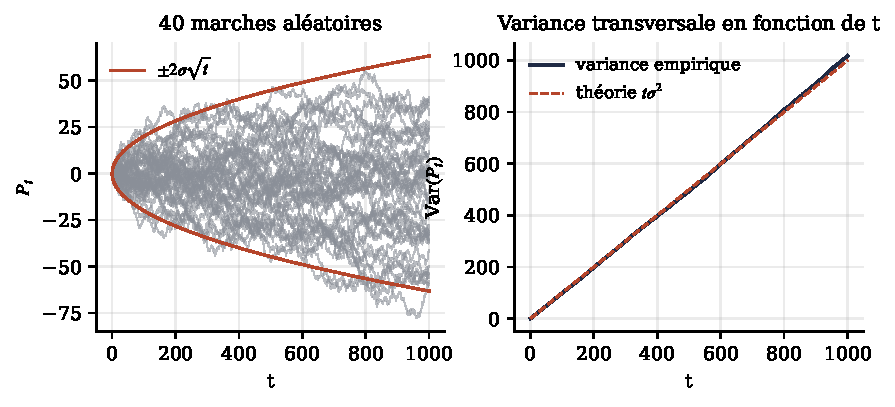
\includegraphics[width=0.92\textwidth]{ch01/h1_random_walk_variance.pdf}
\caption{À gauche, 40 marches aléatoires et l'enveloppe $\pm 2\sigma\sqrt{t}$. À droite, la variance transversale mesurée sur 20\,000 trajectoires suit la droite théorique $t\sigma^2$.}
\label{c1:fig:h1}
\end{figure}

\subsection{Prix, log-prix et rendements}
En pratique on modélise plutôt le \emph{logarithme} du prix comme une marche aléatoire (éventuellement avec une dérive $c$) : $\log P_t = c + \log P_{t-1} + \varepsilon_t$. Le rendement logarithmique $r_t = \log P_t - \log P_{t-1} = c + \varepsilon_t$ est alors un bruit blanc décalé, donc stationnaire. C'est pourquoi les économètres disent qu'un prix est \og intégré d'ordre 1\fg, noté $I(1)$ : il faut le différencier une fois pour obtenir une série stationnaire, notée $I(0)$. Cette notation sera formalisée au chapitre~4.

% =====================================================================
\section{Le processus autorégressif d'ordre un, AR(1)}
% =====================================================================

\subsection{Définition et résolution}

\begin{definition}
$(X_t)$ suit un AR(1) si $X_t = c + \varphi X_{t-1} + \varepsilon_t$, avec $(\varepsilon_t)$ bruit blanc de variance $\sigma^2$ et $c$, $\varphi$ deux constantes.
\end{definition}

On cherche d'abord le niveau $\mu$ autour duquel le processus pourrait se stabiliser. Si la série était constante égale à $\mu$ en l'absence de choc, on aurait $\mu = c + \varphi\mu$, donc, pour $\varphi \ne 1$,
\[
\mu = \frac{c}{1-\varphi}.
\]
En remplaçant $c = \mu(1-\varphi)$ dans la définition, on obtient la forme \og centrée\fg{}, beaucoup plus parlante :
\begin{equation}\label{c1:eq:ar1c}
X_t - \mu = \varphi\,(X_{t-1}-\mu) + \varepsilon_t.
\end{equation}
Notons $Y_t = X_t - \mu$ l'écart à la moyenne. Alors $Y_t = \varphi Y_{t-1} + \varepsilon_t$, et en remplaçant de proche en proche :
\begin{align*}
Y_t &= \varphi Y_{t-1} + \varepsilon_t = \varphi(\varphi Y_{t-2} + \varepsilon_{t-1}) + \varepsilon_t = \varphi^2 Y_{t-2} + \varphi\varepsilon_{t-1} + \varepsilon_t\\
&= \dots = \varphi^t Y_0 + \sum_{j=0}^{t-1}\varphi^j\,\varepsilon_{t-j}. \tag{$\ast$}
\end{align*}
La formule $(\ast)$ dit tout : l'écart d'aujourd'hui est l'écart initial multiplié par $\varphi^t$, plus une somme de chocs passés dont l'influence décroît géométriquement avec leur ancienneté (le choc d'il y a $j$ périodes pèse $\varphi^j$).

\subsection{Condition de stationnarité et moments}

\begin{proposition}\label{c1:prop:ar1}
Si $|\varphi| < 1$, l'AR(1) admet une solution stationnaire de moyenne $\mu = c/(1-\varphi)$, de variance et d'autocorrélation
\[
\gamma(0) = \frac{\sigma^2}{1-\varphi^2}, \qquad \rho(h) = \varphi^{h}\quad (h\ge0).
\]
Si $\varphi = 1$, le processus est une marche aléatoire (avec dérive $c$) et n'est pas stationnaire.
\end{proposition}
\begin{proof}
\emph{Moyenne.} Si $X$ est stationnaire, $\E X_t = \E X_{t-1} = m$. En prenant l'espérance dans la définition : $m = c + \varphi m$, donc $m = c/(1-\varphi) = \mu$.

\emph{Variance.} Dans \eqref{c1:eq:ar1c}, $\varepsilon_t$ est non corrélé avec $X_{t-1}$ (qui ne dépend que des chocs passés). Par la proposition~\ref{c1:prop:varspread} appliquée avec une covariance nulle : $\Var(X_t) = \varphi^2\Var(X_{t-1}) + \sigma^2$. Si la variance est constante, égale à $v$, alors $v = \varphi^2 v + \sigma^2$, soit $v(1-\varphi^2) = \sigma^2$ et $v = \sigma^2/(1-\varphi^2)$. Cette quantité n'est positive et finie que si $\varphi^2<1$, c'est-à-dire $|\varphi|<1$.

\emph{Autocovariance.} Avec $Y_t = X_t-\mu$, on itère $(\ast)$ sur $h$ pas à partir de $t-h$ : $Y_t = \varphi^h Y_{t-h} + \sum_{j=0}^{h-1}\varphi^j\varepsilon_{t-j}$. Les chocs $\varepsilon_{t-h+1},\dots,\varepsilon_t$ sont non corrélés avec $Y_{t-h}$, donc
\[
\gamma(h) = \Cov(Y_t, Y_{t-h}) = \varphi^h\Var(Y_{t-h}) = \varphi^h\gamma(0), \qquad \rho(h) = \frac{\gamma(h)}{\gamma(0)} = \varphi^h.
\]
\emph{Cas $\varphi=1$.} La définition devient $X_t = c + X_{t-1} + \varepsilon_t$ : c'est une marche aléatoire avec dérive, de variance croissante (proposition~\ref{c1:prop:rw}).
\end{proof}

\subsection{L'écriture \og retour à la moyenne\fg}

On soustrait $X_{t-1}-\mu$ des deux côtés de \eqref{c1:eq:ar1c} :
\begin{equation}\label{c1:eq:ecm}
\underbrace{X_t - X_{t-1}}_{\Delta X_t} = -\underbrace{(1-\varphi)}_{\kappa}\,(X_{t-1}-\mu) + \varepsilon_t.
\end{equation}
Avec $0<\varphi<1$, le coefficient $\kappa = 1-\varphi$ est compris entre 0 et 1 : à chaque période, le processus corrige en moyenne la fraction $\kappa$ de son écart à la moyenne. Si $X_{t-1}$ est au-dessus de $\mu$, la variation attendue est négative ; s'il est en dessous, elle est positive.

\begin{intuition}
Imaginez une balle attachée à un élastique fixé au point $\mu$. À chaque instant, quelqu'un la pousse au hasard (le choc $\varepsilon_t$), mais l'élastique la tire vers $\mu$ avec une force proportionnelle à la distance. Plus $\kappa$ est grand, plus l'élastique est raide. Avec $\varphi = 1$, il n'y a plus d'élastique : on retrouve le promeneur ivre. L'équation \eqref{c1:eq:ecm} préfigure le modèle à correction d'erreur du chapitre~4 et le processus d'Ornstein-Uhlenbeck du chapitre~5, qui en est la version en temps continu.
\end{intuition}

\subsection{La demi-vie}

\begin{proposition}[Demi-vie]\label{c1:prop:hl}
Pour $0<\varphi<1$, l'écart \emph{espéré} à la moyenne est divisé par deux en
\[
h_{1/2} = -\frac{\ln 2}{\ln\varphi} \quad\text{périodes},\qquad\text{avec l'approximation}\qquad h_{1/2} \approx \frac{\ln 2}{1-\varphi}\ \text{ quand } \varphi \text{ est proche de } 1.
\]
\end{proposition}
\begin{proof}
D'après $(\ast)$ appliquée à partir de la date $t$, $Y_{t+h} = \varphi^hY_t + \sum_{j=0}^{h-1}\varphi^j\varepsilon_{t+h-j}$. Les chocs futurs ont une espérance nulle, donc $\E[Y_{t+h}\mid Y_t] = \varphi^h Y_t$. On cherche $h$ tel que $\varphi^h = 1/2$. En prenant le logarithme : $h\ln\varphi = \ln(1/2) = -\ln 2$, d'où $h = -\ln 2/\ln\varphi$ (positif puisque $\ln\varphi<0$). Pour l'approximation, on pose $\varphi = 1-\kappa$ avec $\kappa$ petit ; le développement limité $\ln(1-\kappa) = -\kappa - \kappa^2/2 - \dots \approx -\kappa$ donne $h \approx \ln 2/\kappa$.
\end{proof}

\begin{table}[h]
\centering\small
\caption{Demi-vie en fonction de $\varphi$ (en nombre de périodes, par exemple en jours sur données quotidiennes).}
\label{c1:tab:hl}
\begin{tabular}{lccccc}
\toprule
$\varphi$ & 0,50 & 0,80 & 0,90 & 0,95 & 0,99 \\
\midrule
$h_{1/2}$ exacte $= -\ln2/\ln\varphi$ & 1,00 & 3,11 & 6,58 & 13,51 & 68,97 \\
approximation $\ln 2/(1-\varphi)$ & 1,39 & 3,47 & 6,93 & 13,86 & 69,31 \\
\bottomrule
\end{tabular}
\end{table}

\paragraph{Lecture pour le trading.} La demi-vie donne l'échelle de temps d'une stratégie. Une demi-vie de 6 jours signifie qu'un écart ouvert met typiquement une à deux semaines à se refermer ; une demi-vie de 70 jours immobilise le capital pendant des mois et multiplie les occasions de rupture. \citet{chan2013} recommande d'utiliser la demi-vie pour régler à la fois la fenêtre de calcul de la moyenne mobile et la durée de détention attendue.

\subsection{Vérification (H2)}

\begin{codebox}[ — script \texttt{h2\_ar1\_half\_life.py}]
\textbf{Hypothèses :} pour $\varphi = 0{,}95$ et $\sigma = 1$ : (a) $\gamma(0) = 1/(1-0{,}95^2) = 10{,}256$ ; (b) $\rho(h) = 0{,}95^h$ ; (c) demi-vie $13{,}51$ ; (d) biais de l'estimateur sur échantillon court.

\textbf{Résultats :} (a) variance mesurée sur 200\,000 points : $10{,}355$ ; (b) autocorrélation au retard 10 : $0{,}602$ contre $0{,}599$ en théorie ; (c) sur 20\,000 trajectoires partant d'un écart de 10, l'écart moyen passe sous 5 après $13{,}59$ périodes ; (d) voir le tableau~\ref{c1:tab:bias}.
\end{codebox}

\begin{table}[h]
\centering\small
\caption{Estimation de $\varphi$ et de la demi-vie par moindres carrés sur 2\,000 échantillons simulés ($\varphi = 0{,}95$, vraie demi-vie $13{,}51$).}
\label{c1:tab:bias}
\begin{tabular}{rccccc}
\toprule
Taille $n$ & $\overline{\hat\varphi}$ & biais & demi-vie médiane & quantile 5\,\% & quantile 95\,\% \\
\midrule
250 & 0,9343 & $-0{,}0157$ & 10,82 & 5,87 & 21,38 \\
1\,000 & 0,9460 & $-0{,}0040$ & 12,65 & 9,28 & 17,81 \\
5\,000 & 0,9493 & $-0{,}0007$ & 13,39 & 11,51 & 15,55 \\
\bottomrule
\end{tabular}
\end{table}

\begin{figure}[h]
\centering
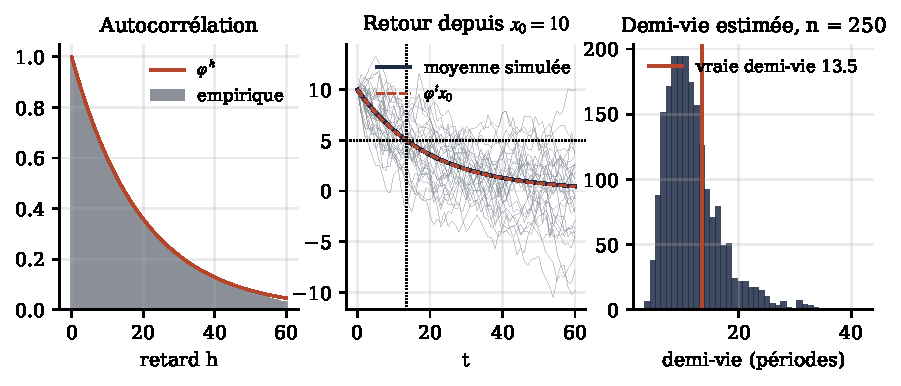
\includegraphics[width=0.98\textwidth]{ch01/h2_ar1_half_life.pdf}
\caption{À gauche, l'autocorrélation empirique suit $\varphi^h$. Au centre, 30 trajectoires partant de $x_0 = 10$ et leur moyenne, qui suit $\varphi^t x_0$ et coupe le niveau 5 à la demi-vie. À droite, la dispersion de la demi-vie estimée sur 250 observations (environ un an de données quotidiennes).}
\label{c1:fig:h2}
\end{figure}

\begin{pitfall}
Avec un an de données quotidiennes ($n = 250$), la demi-vie estimée est en médiane de 10,8 jours au lieu de 13,5, et dans 10\,\% des cas elle sort de l'intervalle $[5{,}9\,;\,21{,}4]$. L'estimateur de $\varphi$ est biaisé vers le bas ; l'approximation classique de \citet{kendall1954}, $\E[\hat\varphi]-\varphi \approx -(1+3\varphi)/n$, prédit $-3{,}85/250 = -0{,}0154$, très proche du biais mesuré ($-0{,}0157$). Conséquence pratique : sur historique court, une paire paraît revenir \emph{plus vite} qu'en réalité, ce qui pousse à trader trop souvent et à sous-estimer la durée de détention. Le chapitre~2 revient sur ce biais et le chapitre~5 sur l'estimation par maximum de vraisemblance.
\end{pitfall}

% =====================================================================
\section{De deux prix non stationnaires à un écart stationnaire}\label{c1:sec:coint}
% =====================================================================

\subsection{L'ivrogne et son chien}

\citet{murray1994} propose l'image suivante. Une promeneuse ivre sort du bar et erre au hasard : sa position est une marche aléatoire. Son chien, en laisse, erre lui aussi. Prise isolément, la trajectoire de chacun est imprévisible. Mais la laisse impose que la distance entre les deux reste bornée : quand le chien s'éloigne trop, la promeneuse l'appelle, ou le chien revient de lui-même. La \emph{distance} entre eux est stationnaire, alors que leurs \emph{positions} ne le sont pas.

\begin{definition}[Cointégration, version intuitive]
Deux séries $X_t$ et $Y_t$ non stationnaires de type $I(1)$ sont \emph{cointégrées} s'il existe un nombre $\beta$ tel que l'écart $S_t = Y_t - \beta X_t$ soit stationnaire. Le vecteur $(1,-\beta)$ est appelé vecteur de cointégration. La définition formelle, les tests et les généralisations à plusieurs actifs sont l'objet du chapitre~4 \citep{englegranger1987,johansen1991}.
\end{definition}

Voilà l'idée fondatrice de l'arbitrage statistique par cointégration : on ne sait pas prédire $X$ ni $Y$, mais si $S$ est stationnaire, on sait que ses écarts à la moyenne sont temporaires, et la section précédente nous dit à quelle vitesse ils se résorbent.

\subsection{Corrélation n'est pas cointégration}

C'est l'erreur la plus fréquente chez les débutants : choisir des paires parce que leurs rendements sont fortement corrélés. La corrélation des rendements mesure si les deux actifs bougent \emph{dans le même sens le même jour}. La cointégration mesure si leurs \emph{niveaux} restent liés \emph{à long terme}. Les deux propriétés sont logiquement indépendantes.

\begin{example}[Deux paires construites pour le montrer]
\textbf{Paire A} : $X$ et $Y$ sont deux marches aléatoires dont les chocs quotidiens sont corrélés à $0{,}9$. Elles bougent presque toujours ensemble, mais rien ne ramène l'une vers l'autre : leur écart est lui-même une marche aléatoire.

\textbf{Paire B} : $X$ est une marche aléatoire et $Y_t = X_t + s_t$, où $s_t$ est un AR(1) avec $\varphi = 0{,}5$ et des chocs d'écart-type $\sigma_s = 2$, plus grand que celui des chocs de $X$ (égal à 1). L'écart $Y - X = s$ est stationnaire, mais les rendements de $Y$ sont dominés par le bruit de $s$.
\end{example}

On peut même calculer la corrélation des rendements de la paire B. Les rendements sont $\Delta X_t = u_t$ et $\Delta Y_t = u_t + \Delta s_t$. Calculons d'abord la variance de $\Delta s_t = s_t - s_{t-1}$ par la proposition~\ref{c1:prop:varspread} (avec $\beta = 1$) et la proposition~\ref{c1:prop:ar1} :
\[
\Var(\Delta s_t) = \gamma(0) + \gamma(0) - 2\gamma(1) = 2\gamma(0)(1-\varphi), \qquad \gamma(0) = \frac{\sigma_s^2}{1-\varphi^2} = \frac{4}{0{,}75} = 5{,}33,
\]
donc $\Var(\Delta s_t) = 2\times 5{,}33\times 0{,}5 = 5{,}33$. Comme $u_t$ est indépendant de $s$, $\Cov(\Delta X_t,\Delta Y_t) = \Var(u_t) = 1$ et $\Var(\Delta Y_t) = 1 + 5{,}33 = 6{,}33$. D'où
\[
\Corr(\Delta X_t,\Delta Y_t) = \frac{1}{\sqrt{1}\sqrt{6{,}33}} \approx 0{,}397.
\]

\begin{codebox}[ — script \texttt{h3\_correlation\_vs\_cointegration.py}]
\textbf{Hypothèse :} forte corrélation des rendements sans cointégration (A) et faible corrélation avec cointégration (B) sont possibles. \textbf{Protocole :} 1\,000 jours par paire ; test ADF sur l'écart $Y-X$ (utilisé ici comme boîte noire, il sera étudié au chapitre~3) ; 500 répétitions. \textbf{Résultats :} paire A : corrélation moyenne des rendements $0{,}90$, le test conclut à la stationnarité de l'écart dans seulement $5{,}8\,\%$ des cas, ce qui correspond au taux de fausses alertes attendu d'un test à 5\,\%. Paire B : corrélation moyenne $0{,}395$ (le calcul théorique donnait $0{,}397$), et le test conclut à la stationnarité dans $100\,\%$ des cas.
\end{codebox}

\begin{figure}[h]
\centering
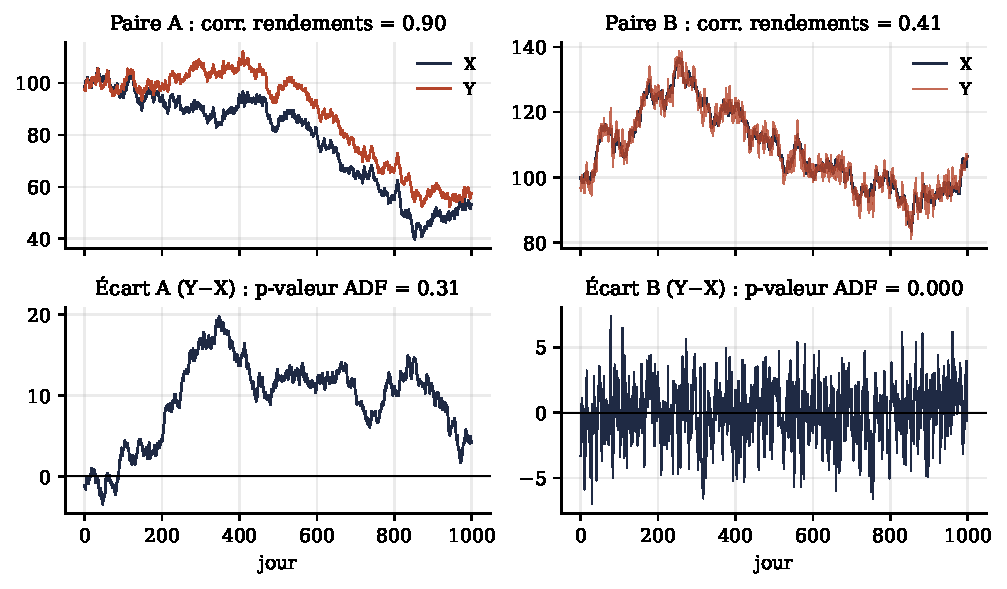
\includegraphics[width=0.9\textwidth]{ch01/h3_correlation_vs_cointegration.pdf}
\caption{En haut, les prix des deux paires ; en bas, leurs écarts. La paire A, très corrélée, dérive sans retour ; la paire B, peu corrélée, a un écart qui oscille autour de zéro.}
\label{c1:fig:h3}
\end{figure}

\subsection{Le piège de la régression fallacieuse}\label{c1:sec:spurious}

Si l'on régresse un prix sur un autre pour trouver $\beta$, on risque de \og découvrir\fg{} une relation qui n'existe pas. \citet{granger1974} ont montré que la régression d'une marche aléatoire sur une autre, \emph{indépendante}, produit très souvent une pente \og significative\fg{} au sens du test de Student usuel et un $R^2$ élevé. La raison : les deux séries ont des tendances aléatoires qui, sur un échantillon fini, semblent aller dans le même sens ou en sens opposé, et les hypothèses du test de Student (résidus non corrélés et stationnaires) sont violées.

\begin{codebox}[ — script \texttt{h4\_spurious\_regression.py}]
\textbf{Hypothèse :} régresser deux marches aléatoires indépendantes rejette \og pente nulle\fg{} bien plus souvent que 5\,\%. \textbf{Protocole :} 2\,000 répétitions, $n = 500$. \textbf{Résultats :} régression en niveaux : la pente est déclarée significative à 5\,\% dans $89\,\%$ des cas, le $R^2$ médian vaut $0{,}17$ et dépasse $0{,}3$ dans $35\,\%$ des cas. Régression des rendements : $4{,}3\,\%$ de rejets, conforme aux 5\,\% attendus, et $R^2$ médian de $0{,}0009$.
\end{codebox}

\begin{figure}[h]
\centering
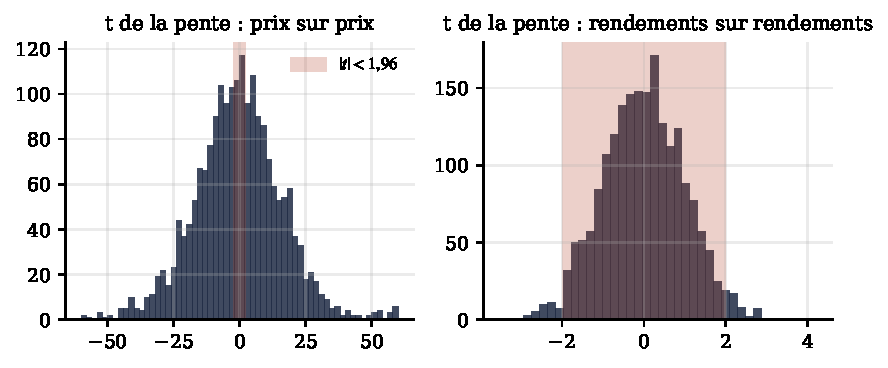
\includegraphics[width=0.85\textwidth]{ch01/h4_spurious_regression.pdf}
\caption{Distribution de la statistique $t$ de la pente. En niveaux (gauche), elle est très dispersée et sort presque toujours de la zone $|t|<1{,}96$ ; en rendements (droite), elle suit à peu près une loi normale centrée réduite.}
\label{c1:fig:h4}
\end{figure}

\begin{pitfall}
Une régression de prix sur prix ne prouve rien par elle-même. Elle n'a de sens que si l'on vérifie ensuite que les \emph{résidus} sont stationnaires : c'est exactement la méthode d'Engle et Granger, qui utilise des valeurs critiques spécifiques justement parce que les tests usuels sont faussés dans ce contexte (chapitre~4).
\end{pitfall}

% =====================================================================
\section{Du spread au signal : une première règle de trading}
% =====================================================================

\subsection{Construction sans information future}

On dispose de deux séries de prix $X_t$ et $Y_t$. On coupe l'historique en deux : une \emph{période de formation} (les $n_f$ premières dates) et une \emph{période de trading} (les suivantes). Tout ce qui est estimé l'est \emph{uniquement} sur la formation.
\begin{enumerate}
\item Sur la formation, on estime $Y_t = \alpha + \beta X_t + e_t$ par moindres carrés (proposition~\ref{c1:prop:hedge}), d'où $\hat\alpha$, $\hat\beta$, puis la moyenne $m$ et l'écart-type $d$ des résidus.
\item Sur la période de trading, on calcule l'écart $S_t = Y_t - \hat\beta X_t - \hat\alpha$ et le \emph{z-score} $z_t = (S_t - m)/d$.
\item Règle : si l'on n'a pas de position et $z_t > 2$, on \emph{vend} l'écart (on vend une unité de $Y$ et on achète $\hat\beta$ unités de $X$) ; si $z_t < -2$, on \emph{achète} l'écart ; on sort quand $z_t$ repasse par 0.
\end{enumerate}

\subsection{Comptabilité du gain et des coûts}

Notons $q_t \in \{-1, 0, +1\}$ la position en écart décidée à la clôture de la date $t$. Le gain de la date $t$ à la date $t+1$ est
\[
\text{G}_{t+1} = q_t\,(S_{t+1} - S_t).
\]
Le décalage d'indice est essentiel : la position décidée avec l'information de la date $t$ s'applique à la variation \emph{suivante}. Écrire $q_{t+1}(S_{t+1}-S_t)$ reviendrait à utiliser le prix de demain pour décider aujourd'hui, l'erreur d'anticipation (\emph{look-ahead bias}) la plus fréquente dans les \emph{backtests} amateurs. À chaque changement de position, on paie un coût proportionnel au notionnel échangé sur les deux jambes :
\[
\text{coût}_t = c\;|q_t - q_{t-1}|\;\big(Y_t + |\hat\beta|X_t\big),
\]
où $c$ est exprimé en fraction (5 pb $= 0{,}0005$).

\subsection{Test dans un monde simulé (H5)}

Pour isoler l'effet de chaque ingrédient, on teste la règle dans un monde où la vérité est connue : $X$ est une marche aléatoire autour de 100, $Y_t = 1{,}5\,X_t + s_t$ et $s_t$ est un AR(1) avec $\varphi = 0{,}9$ (demi-vie de 6,6 jours) et des chocs d'écart-type 1. La formation dure 500 jours, le trading 1\,000 jours, et l'on répète l'expérience 400 fois.

\begin{codebox}[ — script \texttt{h5\_zscore\_toy\_strategy.py}]
\textbf{Estimation :} $\hat\beta$ vaut en moyenne $1{,}4999$ (écart-type $0{,}058$) : la régression retrouve bien le vrai ratio \emph{quand la paire est réellement cointégrée}. \textbf{Gain et coûts :} voir le tableau~\ref{c1:tab:h5}. \textbf{Rupture :} dans une seconde série de mondes, l'écart devient une marche aléatoire ($\varphi = 1$) au 200\textsuperscript{e} jour de trading ; on compare les résultats réalisés \emph{après} ce jour (tableau~\ref{c1:tab:h5b}).
\end{codebox}

\begin{table}[h]
\centering\small
\caption{Règle $|z|>2$, sortie à $z = 0$, relation stable. Moyennes sur 400 mondes simulés ; gain exprimé en dollars pour une unité d'écart.}
\label{c1:tab:h5}
\begin{tabular}{rcccc}
\toprule
Coût par jambe & Gain moyen & Part des mondes gagnants & Sharpe annualisé médian & Allers-retours \\
\midrule
0 pb & 70,25 & 100\,\% & 2,02 & 13,3 \\
5 pb & 66,21 & 100\,\% & 1,91 & 13,3 \\
10 pb & 62,17 & 100\,\% & 1,80 & 13,3 \\
25 pb & 50,06 & 100\,\% & 1,45 & 13,3 \\
50 pb & 29,88 & 98,8\,\% & 0,84 & 13,3 \\
\bottomrule
\end{tabular}
\end{table}

\begin{table}[h]
\centering\small
\caption{Après le 200\textsuperscript{e} jour de trading, coût de 5 pb par jambe : relation stable contre relation rompue.}
\label{c1:tab:h5b}
\begin{tabular}{lcc}
\toprule
 & Relation stable & Relation rompue \\
\midrule
Gain moyen par monde & 53,41 & $-2{,}09$ (erreur-type 1,27) \\
Quantile 5\,\% du gain & 27,64 & $-46{,}66$ \\
Part des trades gagnants & 99,1\,\% & 78,0\,\% \\
Gain moyen d'un trade gagnant & 5,01 & 5,17 \\
Perte moyenne d'un trade perdant & $-1{,}73$ & $-20{,}40$ \\
Pire trade & $-5{,}57$ & $-83{,}76$ \\
\bottomrule
\end{tabular}
\end{table}

\begin{figure}[h]
\centering
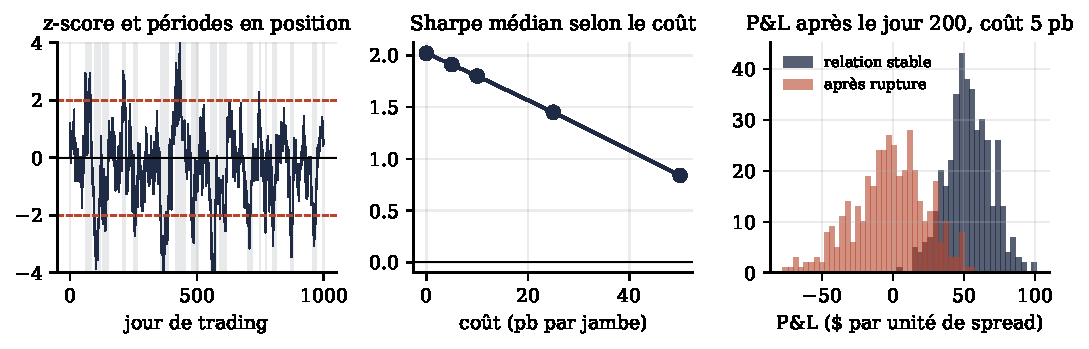
\includegraphics[width=0.98\textwidth]{ch01/h5_zscore_toy_strategy.pdf}
\caption{À gauche, le \emph{z-score} d'un monde simulé, les seuils $\pm 2$ et les périodes en position (grisées). Au centre, le Sharpe médian baisse avec le coût. À droite, distribution du gain réalisé après le 200\textsuperscript{e} jour, avec et sans rupture.}
\label{c1:fig:h5}
\end{figure}

\needspace{8\baselineskip}
\paragraph{Ce que montrent les chiffres.}
\begin{enumerate}
\item \emph{Quand l'écart est réellement stationnaire, la règle gagne.} Chaque aller-retour capture environ deux écarts-types de l'écart ($2\times\sqrt{1/(1-0{,}81)} \approx 4{,}6$), ce qui correspond au gain moyen par trade d'environ 5.
\item \emph{Les coûts mordent vite.} Un aller-retour échange quatre fois un notionnel d'environ 150 (deux jambes, entrée et sortie), soit environ 600 ; à 5 pb, cela coûte $0{,}30$ par aller-retour, ce qui explique la baisse de $70{,}25$ à $66{,}21$ sur 13,3 allers-retours. À 50 pb, le Sharpe est divisé par plus de deux.
\item \emph{Un fort taux de réussite ne prouve rien.} Après la rupture, 78\,\% des trades restent gagnants, mais la perte moyenne d'un trade perdant ($-20{,}4$) est quatre fois le gain moyen d'un trade gagnant, et le gain total moyen devient statistiquement indiscernable de zéro (moins les coûts). C'est le profil \og ramasser des pièces devant un rouleau compresseur\fg{} : une règle de retour à la moyenne sans contrôle de rupture continue d'accumuler une position perdante en attendant un retour qui ne vient plus.
\end{enumerate}

\begin{pitfall}
Ces résultats proviennent d'un monde simulé \emph{construit pour que la stratégie fonctionne} : écart parfaitement stationnaire, paramètres constants, chocs gaussiens, exécution au prix de clôture, pas de coût d'emprunt des titres vendus à découvert. Sur données réelles, chacun de ces points dégrade la performance. Le monde simulé sert à mesurer l'effet d'un ingrédient à la fois ; il ne prédit pas la rentabilité d'une paire réelle.
\end{pitfall}

% =====================================================================
\section{Ce que la théorie apporte, et ses limites}
% =====================================================================

\paragraph{Ce qu'elle apporte.} Un langage précis : on ne dit plus \og ces deux actions se ressemblent\fg, mais \og l'écart est-il stationnaire, avec quelle demi-vie et quelle variance ?\fg. Des ordres de grandeur avant tout \emph{backtest} : la variance minimale d'un écart ($\sigma_Y^2(1-\rho^2)$), le gain par aller-retour ($\approx$ deux écarts-types de l'écart) et le coût par aller-retour se calculent à la main et disent tout de suite si une idée a une chance de survivre aux frais. Des tests pour éviter les illusions statistiques les plus courantes (régression fallacieuse, corrélation confondue avec cointégration).

\paragraph{Ses limites.}
\begin{itemize}
\item \textbf{La stationnarité ne se démontre jamais sur données.} Un test peut seulement dire que les données sont compatibles avec elle, et sur des échantillons courts la puissance des tests est faible (chapitre~3).
\item \textbf{Les paramètres changent.} $\beta$, $\varphi$ et $\sigma$ dérivent avec les régimes de marché ; une relation solide pendant cinq ans peut se rompre en une semaine (fusion, changement de modèle économique, choc réglementaire). Les chapitres~8 (Kalman) et~17 (détection de rupture) y répondent en partie.
\item \textbf{Les chocs ne sont pas gaussiens.} Les rendements financiers ont des queues épaisses : un écart à $4\sigma$ est beaucoup plus fréquent que $0{,}006\,\%$ du temps. Les seuils fondés sur la loi normale sous-estiment le risque extrême.
\item \textbf{Les frictions ne sont pas modélisées.} Fourchette achat-vente, impact, coût d'emprunt des titres, financement des positions, latence et exécution partielle sont traités dans la partie~III.
\item \textbf{La recherche de paires crée des faux positifs.} Tester 1\,000 paires au seuil de 5\,\% produit en moyenne 50 \og paires cointégrées\fg{} par pur hasard (chapitre~16).
\end{itemize}

% =====================================================================
\section{Fiche à recopier au tableau blanc}
% =====================================================================

\begin{whiteboard}
\begin{itemize}[leftmargin=1.2em]
\item \textbf{Arbitrage pur :} coût $\le 0$, perte impossible, gain possible. \textbf{Statistique :} $v(0)=0$, $\E[v(t)]\to>0$, $\Prob(v(t)<0)\to0$, $\Var(v(t))/t\to0$.
\item \textbf{Variance d'un écart :} $\Var(Y-\beta X) = \sigma_Y^2 + \beta^2\sigma_X^2 - 2\beta\Cov(X,Y)$.
\item \textbf{Couverture optimale :} $\beta^\star = \Cov(X,Y)/\sigma_X^2 = \rho\,\sigma_Y/\sigma_X$ ; variance restante $\sigma_Y^2(1-\rho^2)$.
\item \textbf{Stationnarité faible :} $\E X_t = \mu$, $\Var X_t = \gamma(0)$, $\Cov(X_t,X_{t-h}) = \gamma(h)$, indépendants de $t$.
\item \textbf{Marche aléatoire :} $P_t = P_0 + \sum\varepsilon_i$ ; $\E P_t = P_0$ ; $\Var P_t = t\sigma^2$ ; non stationnaire ; $I(1)$.
\item \textbf{AR(1) :} $X_t - \mu = \varphi(X_{t-1}-\mu) + \varepsilon_t$ ; stationnaire si $|\varphi|<1$ ; $\mu = c/(1-\varphi)$ ; $\gamma(0) = \sigma^2/(1-\varphi^2)$ ; $\rho(h) = \varphi^h$.
\item \textbf{Retour à la moyenne :} $\Delta X_t = -(1-\varphi)(X_{t-1}-\mu) + \varepsilon_t$.
\item \textbf{Demi-vie :} $h_{1/2} = -\ln2/\ln\varphi \approx \ln 2/(1-\varphi)$.
\item \textbf{Cointégration (intuition) :} $X, Y \sim I(1)$ et $Y - \beta X \sim I(0)$.
\item \textbf{Z-score :} $z_t = (S_t - m)/d$, avec $m$, $d$ estimés \emph{sur la formation seulement}.
\item \textbf{Gain sans anticipation :} $G_{t+1} = q_t(S_{t+1}-S_t)$.
\end{itemize}
\end{whiteboard}

% =====================================================================
\section{Exercices}
% =====================================================================

\begin{exercise}
Montrez que $\Var(aX + bY) = a^2\sigma_X^2 + b^2\sigma_Y^2 + 2ab\Cov(X,Y)$, puis retrouvez la proposition~\ref{c1:prop:varspread} comme cas particulier.
\end{exercise}

\begin{exercise}
Deux actifs ont des volatilités quotidiennes $\sigma_X = 1{,}2\,\%$ et $\sigma_Y = 1{,}5\,\%$ et une corrélation de $0{,}85$. Calculez $\beta^\star$ et la volatilité quotidienne de l'écart couvert. Quelle corrélation faudrait-il pour que cette volatilité tombe sous $0{,}3\,\%$ ?
\end{exercise}

\begin{exercise}
Sur données quotidiennes, on estime $\hat\varphi = 0{,}98$. Calculez la demi-vie exacte et approchée. Quel $\varphi$ correspond à une demi-vie de 10 jours ? En utilisant le tableau~\ref{c1:tab:bias}, discutez la fiabilité de cette estimation si elle repose sur un an de données.
\end{exercise}

\begin{exercise}
Montrez que l'AR(1) avec $\varphi = -0{,}5$ est stationnaire. Que vaut son autocorrélation aux retards 1, 2 et 3 ? Décrivez l'allure d'une trajectoire et ce que cela signifierait pour un trader.
\end{exercise}

\begin{exercise}
Démontrez que, pour une marche aléatoire, $\Corr(P_t,P_{t+h}) = \sqrt{t/(t+h)}$, et calculez cette corrélation pour $t = 250$ et $h = 5$. Pourquoi cette valeur proche de 1 n'indique-t-elle aucune prévisibilité exploitable ?
\end{exercise}

\begin{exercise}[à coder]
Modifiez \texttt{h5\_zscore\_toy\_strategy.py} pour tester des seuils d'entrée de 1 ; 1,5 ; 2 ; 2,5 et 3. Quel seuil donne le meilleur Sharpe à 5 pb ? Pourquoi serait-il dangereux de retenir ce seuil sur données réelles si on l'a choisi sur la même période que celle où on mesure la performance ? (Indice : chapitre~16.)
\end{exercise}

\begin{exercise}[à coder]
Ajoutez à \texttt{h5} un stop-loss : on ferme la position si $|z_t| > 4$. Mesurez son effet dans le monde stable et dans le monde avec rupture. Le stop-loss coûte-t-il quelque chose quand la relation est stable ?
\end{exercise}

\begin{exercise}[données réelles]
Téléchargez les prix quotidiens de deux ETF adossés à l'or (par exemple via Interactive Brokers). Estimez $\hat\beta$, l'écart, sa demi-vie, et appliquez le test ADF. S'agit-il d'arbitrage statistique ou de quasi-arbitrage au sens de la section~\ref{c1:sec:arb} ? Rapprochez votre réponse du moteur \texttt{atjte} (chapitre~0, section~\ref{c0:atjte}).
\end{exercise}

% =====================================================================
\section{Pour aller plus loin}
% =====================================================================

\begin{toread}
\begin{itemize}[leftmargin=1.2em]
\item \citet{hamilton1994}, chapitre~3, sections 3.1 (espérance, stationnarité, ergodicité), 3.2 (bruit blanc) et 3.4 (processus autorégressifs) : la référence pour les démonstrations de la section~6.
\item \citet{tsay2010}, chapitre~2, sections sur la stationnarité, l'autocorrélation, le bruit blanc et les modèles AR simples : même contenu, orienté données financières, avec des exemples.
\item \citet{chan2013}, chapitre~2 (\og The Basics of Mean Reversion\fg) : stationnarité, demi-vie et cointégration vues par un praticien, avec code.
\item \citet{murray1994} : trois pages, l'image de l'ivrogne et du chien ; à lire en entier.
\item \citet{hogan2004} : la section qui définit l'arbitrage statistique (définition~\ref{c1:def:statarb} de ce chapitre).
\item \citet{granger1974} : l'article original sur la régression fallacieuse, court et lisible.
\item Chapitre~0, section~\ref{c0:litt} : la revue de littérature, pour situer la suite.
\end{itemize}
\end{toread}

\paragraph{Prochain chapitre.} Le chapitre~2 dérive les moindres carrés sous forme matricielle, explique pourquoi régresser $Y$ sur $X$ ne donne pas le même ratio que régresser $X$ sur $Y$, introduit le maximum de vraisemblance et revient sur le biais de petit échantillon mesuré au tableau~\ref{c1:tab:bias}.

\section{Scripts du chapitre}

\begin{center}\small
\begin{tabular}{ll}
\toprule
Élément & Script (\texttt{code/ch01/}) \\
\midrule
Figure~\ref{c1:fig:h1} & \texttt{h1\_random\_walk\_variance.py} \\
Figure~\ref{c1:fig:h2}, tableau~\ref{c1:tab:bias} & \texttt{h2\_ar1\_half\_life.py} \\
Figure~\ref{c1:fig:h3} & \texttt{h3\_correlation\_vs\_cointegration.py} \\
Figure~\ref{c1:fig:h4} & \texttt{h4\_spurious\_regression.py} \\
Figure~\ref{c1:fig:h5}, tableaux~\ref{c1:tab:h5} et~\ref{c1:tab:h5b} & \texttt{h5\_zscore\_toy\_strategy.py} \\
\bottomrule
\end{tabular}
\end{center}

\noindent Chaque script écrit ses chiffres dans \texttt{code/ch01/results/} sous le même nom avec l'extension \texttt{.json}. Pour tout relancer : \texttt{cd code/ch01 \&\& for f in h*.py; do python \$f; done} (dépendances : \texttt{numpy}, \texttt{matplotlib}, \texttt{statsmodels}).

\subsection*{Estimer une demi-vie en quatre lignes}

\begin{lstlisting}[language=Python]
import numpy as np
def half_life(x):
    """Demi-vie (en periodes) estimee par MCO de x_t sur x_{t-1}."""
    b = np.polyfit(x[:-1], x[1:], 1)[0]     # pente = phi estime
    return -np.log(2) / np.log(b) if 0 < b < 1 else np.inf
\end{lstlisting}


% =====================================================================
\chapter{Régression et estimation}
\label{ch:2}
% =====================================================================

\section{Objectifs et organisation du chapitre}

\paragraph{Objectifs.} Le chapitre~1 a montré que le ratio de couverture à variance minimale est une pente de régression. Ce chapitre donne les outils pour estimer ces pentes correctement et pour savoir quand faire confiance au résultat. À la fin du chapitre, vous saurez : (1) dériver les moindres carrés ordinaires sous forme scalaire et matricielle ; (2) énoncer les hypothèses qui rendent l'estimateur sans biais et ses erreurs-types valides ; (3) corriger les erreurs-types quand les résidus sont autocorrélés (Newey-West) ; (4) expliquer pourquoi régresser $Y$ sur $X$ ne donne pas le même ratio que régresser $X$ sur $Y$, et calculer la régression orthogonale ; (5) écrire et maximiser une vraisemblance, en particulier celle de l'AR(1) ; (6) corriger le biais de petit échantillon du coefficient autorégressif.

\paragraph{Code.} Toutes les vérifications sont dans \texttt{code/ch02/ch02\_regression.py} (expériences E1 à E5), résultats dans \texttt{code/ch02/results.json}.

% =====================================================================
\section{Le modèle linéaire et les moindres carrés}
% =====================================================================

\subsection{Cas d'une seule variable explicative}

On observe $n$ couples $(x_i, y_i)$ et l'on postule $y_i = a + b\,x_i + e_i$, où $e_i$ est un résidu. Les moindres carrés ordinaires (MCO) choisissent $(a,b)$ qui minimisent la somme des carrés des résidus
\[
S(a,b) = \sum_{i=1}^n (y_i - a - b x_i)^2.
\]

\begin{proposition}\label{c2:prop:ols1}
Le minimum est atteint en $\hat b = \dfrac{\sum_i (x_i-\bar x)(y_i-\bar y)}{\sum_i (x_i-\bar x)^2}$ et $\hat a = \bar y - \hat b\,\bar x$.
\end{proposition}
\begin{proof}
$S$ est une fonction convexe de $(a,b)$ (somme de carrés de fonctions affines), donc son minimum annule ses deux dérivées partielles.
\begin{align*}
\frac{\partial S}{\partial a} &= -2\sum_i (y_i - a - b x_i) = 0 \;\Rightarrow\; \sum_i y_i = n a + b\sum_i x_i \;\Rightarrow\; a = \bar y - b\bar x.\\
\frac{\partial S}{\partial b} &= -2\sum_i x_i(y_i - a - b x_i) = 0.
\end{align*}
On remplace $a$ par $\bar y - b\bar x$ dans la seconde équation : $\sum_i x_i\big((y_i-\bar y) - b(x_i-\bar x)\big) = 0$. Comme $\sum_i \bar x\,(y_i - \bar y) = 0$ et $\sum_i\bar x\,(x_i-\bar x) = 0$, on peut remplacer $x_i$ par $x_i - \bar x$ devant la parenthèse sans changer la somme : $\sum_i (x_i-\bar x)(y_i-\bar y) = b\sum_i(x_i-\bar x)^2$, d'où $\hat b$.
\end{proof}

En divisant numérateur et dénominateur par $n-1$, on reconnaît $\hat b = \widehat{\Cov}(X,Y)/\widehat{\Var}(X)$ : c'est la version empirique du ratio de couverture optimal de la proposition~\ref{c1:prop:hedge}.

\subsection{Forme matricielle}

Avec $k$ variables explicatives (dont la constante), on empile les observations : $y \in \R^n$, $X \in \R^{n\times k}$ (une ligne par date, une colonne par variable, la première colonne remplie de 1), $\beta \in \R^k$. Le modèle s'écrit $y = X\beta + \varepsilon$.

\begin{proposition}[Équations normales]\label{c2:prop:olsmat}
Si $X^\top X$ est inversible, l'estimateur des MCO est $\hat\beta = (X^\top X)^{-1}X^\top y$, et les résidus $e = y - X\hat\beta$ vérifient $X^\top e = 0$.
\end{proposition}
\begin{proof}
La somme des carrés vaut $S(b) = (y-Xb)^\top(y-Xb) = y^\top y - 2b^\top X^\top y + b^\top X^\top X b$ (on a utilisé $y^\top Xb = b^\top X^\top y$, car c'est un nombre, égal à son transposé). Le gradient par rapport à $b$ est $\nabla S = -2X^\top y + 2X^\top X b$ (règles $\nabla_b(b^\top c) = c$ et $\nabla_b(b^\top Ab) = 2Ab$ pour $A$ symétrique). L'annuler donne $X^\top X\hat\beta = X^\top y$, puis $\hat\beta = (X^\top X)^{-1}X^\top y$. Enfin $X^\top e = X^\top y - X^\top X\hat\beta = 0$ par les équations normales elles-mêmes.
\end{proof}

\begin{intuition}
$X\hat\beta$ est l'ombre de $y$ projetée sur le plan engendré par les colonnes de $X$, comme l'ombre d'un bâton au soleil de midi sur le sol. Le résidu $e$ est la partie verticale, perpendiculaire au sol : c'est exactement ce que dit $X^\top e = 0$. En \emph{pairs trading}, le résidu de la régression de $Y$ sur $X$ est le \emph{spread} : la partie de $Y$ que $X$ n'explique pas.
\end{intuition}

\paragraph{Qualité d'ajustement.} Le coefficient de détermination $R^2 = 1 - \sum e_i^2/\sum(y_i-\bar y)^2$ mesure la part de la variance de $y$ expliquée. Avec une seule variable explicative, $R^2 = \hat\rho_{XY}^2$.

\begin{codebox}[ — E1, données réelles KO et PEP]
\textbf{Hypothèse :} les formules écrites à la main donnent les mêmes résultats que \texttt{statsmodels}. \textbf{Protocole :} régression du cours de clôture de Coca-Cola sur celui de PepsiCo, 500 séances (octobre 2024 à octobre 2026). \textbf{Résultats :} $\hat a = 105{,}23$ (erreur-type $4{,}68$), $\hat b = -0{,}2176$ (erreur-type $0{,}0319$), $R^2 = 0{,}0855$, identiques à \texttt{statsmodels} à $4\times10^{-12}$ près ; la plus grande composante de $X^\top e$ vaut $10^{-7}$ (zéro numérique). \textbf{Lecture :} sur ces deux années, les cours de KO et PEP ont évolué en sens opposés (KO a monté, PEP a baissé) ; la \og paire classique\fg{} des manuels n'avait aucune relation positive en niveau. Nous y reviendrons aux chapitres~4 et~7.
\end{codebox}

% =====================================================================
\section{Propriétés statistiques de l'estimateur}
% =====================================================================

\subsection{Hypothèses et absence de biais}

Les propriétés de $\hat\beta$ reposent sur des hypothèses sur le terme d'erreur $\varepsilon$ :
\begin{enumerate}[label=(H\arabic*)]
\item \emph{linéarité} : $y = X\beta + \varepsilon$ ;
\item \emph{rang plein} : $X^\top X$ inversible (aucune variable n'est combinaison linéaire des autres) ;
\item \emph{exogénéité} : $\E[\varepsilon \mid X] = 0$ ;
\item \emph{homoscédasticité et absence d'autocorrélation} : $\E[\varepsilon\varepsilon^\top \mid X] = \sigma^2 I_n$.
\end{enumerate}

\begin{proposition}\label{c2:prop:unbiased}
Sous (H1)–(H3), $\E[\hat\beta\mid X] = \beta$. Sous (H1)–(H4), $\Var(\hat\beta\mid X) = \sigma^2(X^\top X)^{-1}$.
\end{proposition}
\begin{proof}
On remplace $y$ par $X\beta+\varepsilon$ : $\hat\beta = (X^\top X)^{-1}X^\top(X\beta+\varepsilon) = \beta + (X^\top X)^{-1}X^\top\varepsilon$. En prenant l'espérance conditionnelle à $X$ et en utilisant (H3) : $\E[\hat\beta\mid X] = \beta + (X^\top X)^{-1}X^\top\E[\varepsilon\mid X] = \beta$. Pour la variance, $\hat\beta - \beta = A\varepsilon$ avec $A = (X^\top X)^{-1}X^\top$, donc $\Var(\hat\beta\mid X) = A\,\E[\varepsilon\varepsilon^\top\mid X]\,A^\top = \sigma^2AA^\top = \sigma^2(X^\top X)^{-1}X^\top X(X^\top X)^{-1} = \sigma^2(X^\top X)^{-1}$.
\end{proof}

On estime $\sigma^2$ par $\hat\sigma^2 = e^\top e/(n-k)$ ; la division par $n-k$ plutôt que $n$ corrige le fait que $k$ paramètres ont été ajustés sur les mêmes données. Le théorème de Gauss-Markov ajoute que, sous (H1)–(H4), $\hat\beta$ a la plus petite variance parmi tous les estimateurs linéaires sans biais.

\subsection{Le test de Student et ses conditions}

La statistique $t_j = \hat\beta_j/\widehat{\mathrm{se}}(\hat\beta_j)$, où $\widehat{\mathrm{se}}$ est la racine du $j$-ème terme diagonal de $\hat\sigma^2(X^\top X)^{-1}$, suit approximativement une loi normale centrée réduite si $\beta_j = 0$. Ce résultat exige (H4). Or les séries financières violent souvent (H4) : un \emph{spread} qui revient lentement à la moyenne a des résidus fortement autocorrélés. Le chapitre~1 a montré le cas extrême (régression fallacieuse, section~\ref{c1:sec:spurious}) ; même avec des séries stationnaires, l'autocorrélation fausse les erreurs-types.

\subsection{Erreurs-types robustes : Newey-West}

Sans (H4), la variance exacte de $\hat\beta$ est
\[
\Var(\hat\beta\mid X) = (X^\top X)^{-1}\Big(\sum_{t}\sum_{s} x_t x_s^\top\,\E[\varepsilon_t\varepsilon_s]\Big)(X^\top X)^{-1},
\]
où $x_t$ est la $t$-ème ligne de $X$ écrite en colonne. La partie centrale, appelée \og viande\fg{} du \og sandwich\fg, contient les covariances croisées des erreurs. \citet{neweywest1987} l'estiment par
\[
\hat\Omega = \hat\Gamma_0 + \sum_{j=1}^{L}\Big(1-\frac{j}{L+1}\Big)\big(\hat\Gamma_j + \hat\Gamma_j^\top\big), \qquad \hat\Gamma_j = \sum_{t=j+1}^{n} e_t e_{t-j}\,x_t x_{t-j}^\top,
\]
avec $L$ retards. Les poids $1 - j/(L+1)$ décroissent linéairement et garantissent que la matrice estimée reste positive.

\begin{codebox}[ — E5, erreurs-types naïves contre Newey-West]
\textbf{Hypothèse :} quand $x$ et les résidus sont tous deux autocorrélés, le test de Student naïf rejette à tort \og pente nulle\fg{} beaucoup plus souvent que 5\,\%, et Newey-West corrige en partie. \textbf{Protocole :} 2\,000 répétitions ; $x$ et $u$ indépendants, chacun AR(1) avec $\varphi = 0{,}9$ ; $y = 1 + 0\cdot x + u$ ; $n = 250$. \textbf{Résultats :} taux de rejet à 5\,\% : $51{,}6\,\%$ en naïf, $27{,}1\,\%$ avec Newey-West à 4 retards (règle usuelle $L = \lfloor 4(n/100)^{2/9}\rfloor$), $17{,}9\,\%$ avec 20 retards.
\end{codebox}

\begin{pitfall}
Le test naïf trouve une relation significative une fois sur deux entre deux séries indépendantes. Newey-West améliore nettement les choses mais reste loin des 5\,\% nominaux quand la persistance est forte et l'échantillon court. Règle pratique : ne jamais sélectionner une paire ou un signal sur la base d'un $t$ de Student calculé sur des séries persistantes ; utiliser les tests dédiés (chapitres~3 et~4), des erreurs-types robustes et, surtout, une validation hors échantillon (chapitre~16).
\end{pitfall}

% =====================================================================
\section{Quelle variable expliquer ? L'asymétrie de la régression}
% =====================================================================

\subsection{Deux régressions, deux ratios}

Pour un \emph{pairs trade}, il faut choisir quelle jambe joue le rôle de $Y$. Ce choix n'est pas neutre.

\begin{proposition}\label{c2:prop:asym}
Soit $\hat\beta_{Y|X}$ la pente de $Y$ sur $X$ et $\hat\beta_{X|Y}$ celle de $X$ sur $Y$. Alors $\hat\beta_{Y|X}\,\hat\beta_{X|Y} = \hat\rho_{XY}^2$, donc $1/\hat\beta_{X|Y} = \hat\beta_{Y|X}/\hat\rho_{XY}^2$.
\end{proposition}
\begin{proof}
D'après la proposition~\ref{c2:prop:ols1}, $\hat\beta_{Y|X} = \hat s_{XY}/\hat s_X^2$ et, par symétrie, $\hat\beta_{X|Y} = \hat s_{XY}/\hat s_Y^2$. Leur produit vaut $\hat s_{XY}^2/(\hat s_X^2\hat s_Y^2) = \hat\rho_{XY}^2$.
\end{proof}

Si l'on régresse $X$ sur $Y$ puis qu'on inverse la pente pour obtenir un ratio \og en unités de $X$ par unité de $Y$\fg, on obtient un ratio plus grand d'un facteur $1/\hat\rho^2$. Avec $\rho = 0{,}6$, l'écart est de 178\,\%. Seule une corrélation parfaite rend les deux choix équivalents.

\begin{intuition}
Les MCO ne mesurent les erreurs que dans une direction : verticalement quand on explique $Y$, horizontalement quand on explique $X$. Le bruit de la variable placée à droite (la variable explicative) \og aplatit\fg{} la pente vers zéro. C'est l'effet dit d'\emph{atténuation}.
\end{intuition}

\subsection{La régression orthogonale}

Pour traiter les deux actifs symétriquement, on minimise la somme des distances \emph{perpendiculaires} à la droite, ce qui revient à minimiser
\[
g(b) = \frac{s_{YY} - 2b\,s_{XY} + b^2 s_{XX}}{1+b^2},
\]
où $s_{XX}$, $s_{YY}$, $s_{XY}$ sont les variances et la covariance empiriques. En effet, la distance perpendiculaire d'un point à la droite $y = a + bx$ est $|y - a - bx|/\sqrt{1+b^2}$.

\begin{proposition}[Pente orthogonale]\label{c2:prop:tls}
Si $s_{XY} > 0$, le minimum de $g$ est atteint en
\[
\hat b_{\perp} = \frac{(s_{YY}-s_{XX}) + \sqrt{(s_{YY}-s_{XX})^2 + 4s_{XY}^2}}{2\,s_{XY}}.
\]
\end{proposition}
\begin{proof}
Écrivons $g = N/D$. La dérivée s'annule quand $N'D = ND'$, soit
$(-2s_{XY} + 2bs_{XX})(1+b^2) = 2b\,(s_{YY} - 2bs_{XY} + b^2s_{XX})$.
En développant les deux membres, les termes en $b^3s_{XX}$ s'annulent et il reste
$-2s_{XY} + 2s_{XY}b^2 + 2b(s_{XX} - s_{YY}) = 0$, soit l'équation du second degré $s_{XY}b^2 + (s_{XX}-s_{YY})b - s_{XY} = 0$. Son discriminant $(s_{XX}-s_{YY})^2 + 4s_{XY}^2$ est positif ; des deux racines, celle avec le signe $+$ est de même signe que $s_{XY}$ et correspond au minimum (l'autre est le maximum, la direction perpendiculaire).
\end{proof}

La pente orthogonale est la direction du premier vecteur propre de la matrice de covariance de $(X,Y)$ : c'est déjà une analyse en composantes principales, que l'on retrouvera au chapitre~10. Son défaut : elle dépend des unités (doubler le prix de $X$ change le résultat), d'où l'usage fréquent de log-prix ou de prix normalisés.

\begin{codebox}[ — E2, asymétrie et régression orthogonale]
\textbf{Simulation} (vrai $\beta = 1{,}5$, $X$ marche aléatoire, écart AR(1) de paramètre $0{,}9$, $n = 500$, 1\,000 répétitions) : MCO de $Y$ sur $X$ : moyenne $1{,}4986$ (écart-type $0{,}059$) ; inverse de la pente de $X$ sur $Y$ : $1{,}5642$ ($0{,}074$) ; régression orthogonale : $1{,}5445$ ($0{,}067$). \textbf{Variables stationnaires} ($\sigma_X = \sigma_Y = 1$) : pour $\rho = 0{,}3$ ; $0{,}6$ ; $0{,}9$ ; $0{,}99$, on obtient $\hat\beta_{Y|X} = 0{,}287$ ; $0{,}600$ ; $0{,}903$ ; $0{,}989$ et $1/\hat\beta_{X|Y} = 3{,}49$ ; $1{,}70$ ; $1{,}11$ ; $1{,}009$, le produit des deux pentes reproduisant $\rho^2$. \textbf{KO et PEP} (prix) : $-0{,}218$ contre $-2{,}54$ selon le sens, $-0{,}41$ en orthogonal ; les trois ratios n'ont même pas d'ordre de grandeur commun.
\end{codebox}

\begin{figure}[h]
\centering
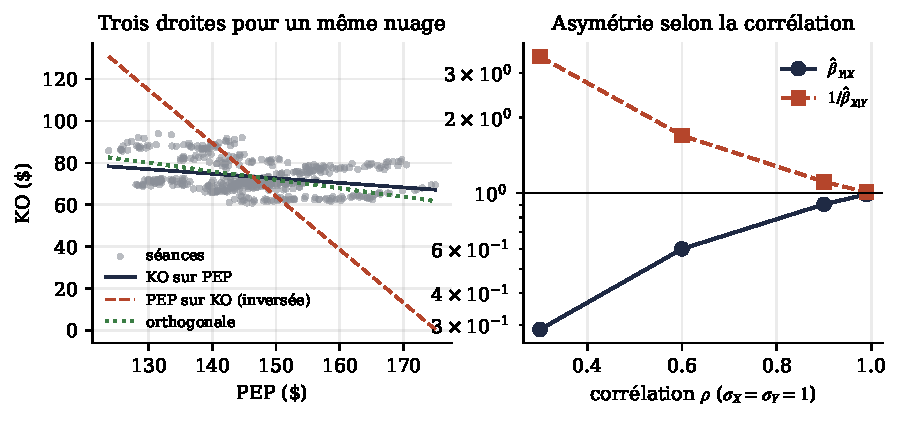
\includegraphics[width=0.95\textwidth]{ch02/asymetrie_regression.pdf}
\caption{À gauche, les cours de KO et PEP (500 séances) et trois droites d'ajustement : selon la méthode, le \og ratio de couverture\fg{} change du tout au tout, signe d'une relation inexistante. À droite, la pente directe et l'inverse de la pente réciproque ne coïncident que si la corrélation est proche de 1 (échelle logarithmique).}
\label{c2:fig:asym}
\end{figure}

\paragraph{Lecture pour le trading.} Quand la paire est réellement cointégrée (simulation), les trois estimateurs sont proches et convergent vers la vraie valeur ; quand elle ne l'est pas (KO/PEP sur cette période), ils divergent. \emph{L'écart entre $\hat\beta_{Y|X}$ et $1/\hat\beta_{X|Y}$ est donc un premier diagnostic gratuit} : s'il est grand, la relation est fragile. Les praticiens retiennent souvent la jambe la plus liquide comme $X$, ou testent les deux sens et gardent celui qui produit l'écart le plus stationnaire (chapitre~4).

\subsection{Prix ou log-prix ? Neutralité en parts ou en dollars}

Régresser les prix donne un ratio en \emph{nombre de parts} : $Y - \beta X$ est la valeur d'un portefeuille long une part de $Y$, court $\beta$ parts de $X$. Régresser les log-prix donne un ratio en \emph{élasticité} : $\log Y - \beta\log X$ ; une position \og neutre en dollars\fg{} (même montant investi des deux côtés) correspond à $\beta = 1$ en log. Le choix change la position et donc le risque : la version en log-prix est la plus courante en actions (on raisonne en rendements), la version en prix est naturelle pour deux instruments du même sous-jacent (or contre or), comme dans \texttt{atjte} où $k$ convertit des unités.

% =====================================================================
\section{Le maximum de vraisemblance}
% =====================================================================

\subsection{Principe}

Soit un modèle qui donne la densité des données $f(x_1,\dots,x_n;\theta)$ en fonction d'un paramètre $\theta$. La \emph{vraisemblance} est cette densité vue comme fonction de $\theta$, à données fixées : $\mathcal L(\theta) = f(x_1,\dots,x_n;\theta)$. L'estimateur du maximum de vraisemblance (MV) est la valeur de $\theta$ qui rend les données observées les plus probables. On maximise en pratique la log-vraisemblance $\ell(\theta) = \ln\mathcal L(\theta)$, plus simple (les produits deviennent des sommes) et qui a le même maximum car $\ln$ est croissante.

\begin{intuition}
Vous trouvez une pièce et la lancez dix fois : huit piles. Quelle probabilité de pile rend ce résultat le plus plausible ? Avec $p = 0{,}5$, huit piles est peu probable ; avec $p = 0{,}8$, c'est le résultat le plus probable. Le maximum de vraisemblance choisit $\hat p = 0{,}8$. C'est le même raisonnement, appliqué à un processus entier.
\end{intuition}

\subsection{Vraisemblance de l'AR(1)}

Pour l'AR(1) gaussien $X_t = c + \varphi X_{t-1} + \varepsilon_t$, $\varepsilon_t\iid\N(0,\sigma^2)$, la loi de $X_t$ \emph{sachant} $X_{t-1}$ est $\N(c+\varphi X_{t-1},\sigma^2)$. Par la formule des probabilités conditionnelles en chaîne, la densité jointe se factorise :
\[
f(x_0,\dots,x_n) = f(x_0)\prod_{t=1}^n f(x_t\mid x_{t-1}).
\]

\begin{proposition}\label{c2:prop:mlear1}
En ignorant le terme $f(x_0)$ (vraisemblance \og conditionnelle\fg), l'estimateur MV de $(c,\varphi)$ est l'estimateur MCO de $x_t$ sur $(1, x_{t-1})$, et $\hat\sigma^2_{MV} = \frac1n\sum_t \hat e_t^2$.
\end{proposition}
\begin{proof}
La log-vraisemblance conditionnelle vaut
\[
\ell(c,\varphi,\sigma^2) = \sum_{t=1}^n \ln\Big[\frac{1}{\sqrt{2\pi\sigma^2}}e^{-\frac{(x_t-c-\varphi x_{t-1})^2}{2\sigma^2}}\Big] = -\frac n2\ln(2\pi\sigma^2) - \frac{1}{2\sigma^2}\sum_{t=1}^n(x_t - c - \varphi x_{t-1})^2.
\]
Pour tout $\sigma^2$ fixé, maximiser en $(c,\varphi)$ revient à minimiser la somme des carrés : ce sont les MCO. On dérive ensuite par rapport à $\sigma^2$ : $-\frac{n}{2\sigma^2} + \frac{1}{2\sigma^4}\sum\hat e_t^2 = 0$, d'où $\hat\sigma^2 = \frac1n\sum\hat e_t^2$.
\end{proof}

La vraisemblance \emph{exacte} ajoute $\ln f(x_0)$, où $X_0 \sim \N\big(c/(1-\varphi),\,\sigma^2/(1-\varphi^2)\big)$ si le processus est stationnaire (proposition~\ref{c1:prop:ar1}). Ce terme pèse peu quand $n$ est grand, mais il pénalise les valeurs de $\varphi$ proches de 1 et améliore légèrement l'estimation sur échantillon court.

\paragraph{Propriétés asymptotiques.} Sous des conditions de régularité, l'estimateur MV est convergent et asymptotiquement normal, de variance égale à l'inverse de l'information de Fisher. Pour l'AR(1) stationnaire, cela donne $\Var(\hat\varphi) \approx (1-\varphi^2)/n$ \citep[ch.~5 et 8]{hamilton1994}.

\begin{codebox}[ — E3, MCO et maximum de vraisemblance]
\textbf{Protocole :} un AR(1) avec $c = 0{,}2$, $\varphi = 0{,}9$, $\sigma = 0{,}5$, $n = 300$ ; maximisation numérique (Nelder-Mead). \textbf{Résultats :} MCO : $\hat c = 0{,}1893$, $\hat\varphi = 0{,}9039$, $\hat\sigma = 0{,}5193$ ; MV conditionnel : exactement les mêmes valeurs ; MV exact : $\hat c = 0{,}1972$, $\hat\varphi = 0{,}9019$, $\hat\sigma = 0{,}5187$. La figure~\ref{c2:fig:ll} montre la log-vraisemblance profilée en $\varphi$.
\end{codebox}

\begin{figure}[h]
\centering
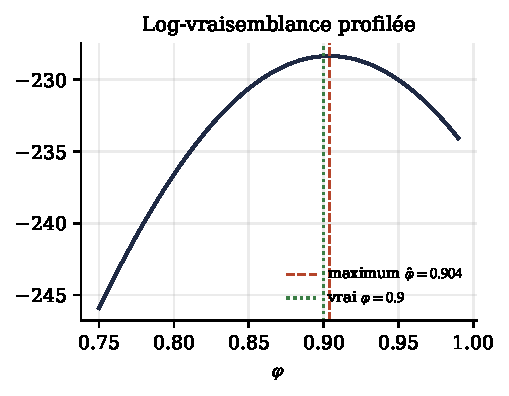
\includegraphics[width=0.48\textwidth]{ch02/vraisemblance_ar1.pdf}
\caption{Log-vraisemblance profilée de l'AR(1) en fonction de $\varphi$ (les autres paramètres sont optimisés pour chaque $\varphi$). Le maximum est proche, mais pas égal, à la vraie valeur : c'est l'incertitude d'estimation.}
\label{c2:fig:ll}
\end{figure}

% =====================================================================
\section{Le biais de petit échantillon et sa correction}
% =====================================================================

Le chapitre~1 (tableau~\ref{c1:tab:bias}) a mesuré que $\hat\varphi$ est biaisé vers le bas. L'approximation de \citet{kendall1954} donne $\E[\hat\varphi] - \varphi \approx -(1+3\varphi)/n$ quand la moyenne est estimée. On peut donc corriger :
\[
\hat\varphi_{c} = \hat\varphi + \frac{1+3\hat\varphi}{n}.
\]
La correction utilise $\hat\varphi$ au lieu de $\varphi$ (inconnu), ce qui laisse un petit biais résiduel.

\begin{codebox}[ — E4, correction de Kendall]
\textbf{Protocole :} $\varphi = 0{,}95$ (demi-vie vraie $13{,}51$), 3\,000 échantillons par taille. \textbf{Résultats} (tableau~\ref{c2:tab:kendall}) : la correction ramène la moyenne de $\hat\varphi$ très près de la vérité et supprime l'essentiel du biais de demi-vie, au prix d'une légère sur-correction de la médiane de la demi-vie quand $n$ est petit.
\end{codebox}

\begin{table}[h]
\centering\small
\caption{Estimation brute et corrigée de $\varphi = 0{,}95$ (moyennes et médianes sur 3\,000 échantillons).}
\label{c2:tab:kendall}
\begin{tabular}{rccccc}
\toprule
$n$ & $\overline{\hat\varphi}$ brut & $\overline{\hat\varphi_c}$ corrigé & demi-vie médiane brute & demi-vie médiane corrigée & écart-type de $\hat\varphi$\\
\midrule
100 & 0,9068 & 0,9430 & 7,92 & 14,61 & 0,0496\\
250 & 0,9336 & 0,9489 & 10,79 & 14,41 & 0,0247\\
1\,000 & 0,9462 & 0,9500 & 12,77 & 13,80 & 0,0105\\
\bottomrule
\end{tabular}
\end{table}

\begin{pitfall}
Corriger le biais ne réduit pas l'incertitude. Avec $n = 250$, l'écart-type de $\hat\varphi$ ($0{,}025$) reste du même ordre que la distance qui sépare $\varphi = 0{,}95$ de la racine unitaire $\varphi = 1$. Autrement dit, un an de données quotidiennes ne permet pas de distinguer de façon fiable un écart qui revient lentement d'un écart qui ne revient pas du tout. Le chapitre~3 quantifie ce problème de puissance.
\end{pitfall}

% =====================================================================
\section{Ce que la théorie apporte, et ses limites}
% =====================================================================

\paragraph{Apports.} Les MCO donnent le ratio de couverture à variance minimale et le \emph{spread} comme résidu ; le maximum de vraisemblance fournit un cadre unique pour estimer tous les modèles du cours (AR, Ornstein-Uhlenbeck, Kalman, copules) ; les erreurs-types robustes et la correction de biais rendent les estimations plus honnêtes.

\paragraph{Limites.} (1) Le ratio estimé dépend du sens de la régression, des unités et de la fenêtre ; il n'existe pas \og le\fg{} bon $\beta$. (2) Les hypothèses (H3)–(H4) sont presque toujours violées par les séries de prix. (3) Les propriétés asymptotiques du MV supposent que le modèle est juste ; si l'écart n'est pas un AR(1), l'estimateur converge vers le \og meilleur AR(1)\fg, pas vers une vérité. (4) Aucun estimateur ne crée de l'information absente des données : la précision est limitée par la longueur de l'échantillon, mesurée en nombre de demi-vies observées plutôt qu'en nombre de points.

% =====================================================================
\section{Fiche à recopier au tableau blanc}
% =====================================================================

\begin{whiteboard}
\begin{itemize}[leftmargin=1.2em]
\item \textbf{MCO simples :} $\hat b = \sum(x-\bar x)(y-\bar y)/\sum(x-\bar x)^2$, $\hat a = \bar y - \hat b\bar x$.
\item \textbf{MCO matriciels :} $\hat\beta = (X^\top X)^{-1}X^\top y$ ; $X^\top e = 0$ ; $\hat\sigma^2 = e^\top e/(n-k)$.
\item \textbf{Sans biais :} $\hat\beta = \beta + (X^\top X)^{-1}X^\top\varepsilon$ ; $\Var(\hat\beta) = \sigma^2(X^\top X)^{-1}$ sous (H4).
\item \textbf{Sandwich :} $(X^\top X)^{-1}\,\hat\Omega\,(X^\top X)^{-1}$ ; Newey-West : poids $1-j/(L+1)$.
\item \textbf{Asymétrie :} $\hat\beta_{Y|X}\hat\beta_{X|Y} = \hat\rho^2$.
\item \textbf{Orthogonale :} $s_{XY}b^2 + (s_{XX}-s_{YY})b - s_{XY} = 0$, racine de même signe que $s_{XY}$.
\item \textbf{Log-vraisemblance AR(1) :} $\ell = -\frac n2\ln(2\pi\sigma^2) - \frac1{2\sigma^2}\sum(x_t - c - \varphi x_{t-1})^2$ ; MV conditionnel $=$ MCO.
\item \textbf{Asymptotique :} $\Var(\hat\varphi)\approx(1-\varphi^2)/n$.
\item \textbf{Correction de Kendall :} $\hat\varphi_c = \hat\varphi + (1+3\hat\varphi)/n$.
\end{itemize}
\end{whiteboard}

% =====================================================================
\section{Exercices}
% =====================================================================

\begin{exercise}
Montrez que, dans la régression simple avec constante, la somme des résidus est nulle et que la droite passe par le point moyen $(\bar x,\bar y)$.
\end{exercise}

\begin{exercise}
Montrez que $R^2 = \hat\rho_{XY}^2$ en régression simple. Déduisez-en la proposition~\ref{c2:prop:asym} par un autre chemin.
\end{exercise}

\begin{exercise}
Vérifiez la proposition~\ref{c2:prop:tls} dans le cas $s_{XX} = s_{YY}$ : que vaut la pente orthogonale ? Interprétez géométriquement.
\end{exercise}

\begin{exercise}
Avec $\varphi = 0{,}95$ et $n = 250$, calculez l'écart-type asymptotique $\sqrt{(1-\varphi^2)/n}$ et comparez à l'écart-type mesuré dans le tableau~\ref{c2:tab:kendall}. Pourquoi l'asymptotique sous-estime-t-elle l'incertitude ?
\end{exercise}

\begin{exercise}[à coder]
Reprenez E2 en régressant $\log$KO sur $\log$PEP sur des fenêtres glissantes de 120 séances. Tracez le ratio dans le temps. Que conclure sur la stabilité de la \og couverture\fg{} ?
\end{exercise}

\begin{exercise}[à coder]
Implémentez un \emph{bootstrap} par blocs pour l'erreur-type de $\hat b$ dans E5 (tirage de blocs consécutifs de 25 observations) et comparez son taux de rejet à celui de Newey-West.
\end{exercise}

% =====================================================================
\section{Pour aller plus loin}
% =====================================================================

\begin{toread}
\begin{itemize}[leftmargin=1.2em]
\item \citet{hamilton1994}, chapitre~8 (\og Linear Regression Models\fg) pour les MCO et leurs propriétés ; chapitre~5 (\og Maximum Likelihood Estimation\fg) pour la vraisemblance des processus ARMA.
\item \citet{neweywest1987} : l'article original, très court, sur l'estimateur de variance robuste.
\item \citet{kendall1954} : la note originale sur le biais d'estimation de l'autocorrélation.
\item \citet{vidyamurthy2004} : la discussion du choix du ratio de couverture en \emph{pairs trading}, avant les tests de cointégration.
\end{itemize}
\end{toread}

\section{Scripts du chapitre}
\noindent\texttt{code/ch02/ch02\_regression.py} : E1 (MCO à la main contre \texttt{statsmodels}), E2 (asymétrie et figure~\ref{c2:fig:asym}), E3 (vraisemblance et figure~\ref{c2:fig:ll}), E4 (tableau~\ref{c2:tab:kendall}), E5 (Newey-West). Résultats : \texttt{code/ch02/results.json}.

% =====================================================================
\chapter{Tester la stationnarité et le retour à la moyenne}
\label{ch:3}
% =====================================================================

\section{Objectifs et organisation du chapitre}

\paragraph{Objectifs.} Les chapitres précédents ont utilisé le test ADF comme une boîte noire. Ce chapitre l'ouvre. À la fin, vous saurez : (1) écrire la régression de Dickey-Fuller et expliquer pourquoi sa statistique ne suit pas une loi de Student ; (2) choisir les termes déterministes (constante, tendance) et le nombre de retards ; (3) évaluer la puissance d'un test et la relier au nombre de demi-vies observées ; (4) utiliser le test KPSS et combiner les deux ; (5) calculer et interpréter le ratio de variance et l'exposant de Hurst ; (6) appliquer ces outils à deux paires réelles et lire correctement des résultats contradictoires.

\paragraph{Code.} \texttt{code/ch03/ch03\_stationarity\_tests.py}, expériences E1 à E6.

% =====================================================================
\section{Le test de Dickey-Fuller}
% =====================================================================

\subsection{La régression}

On part de l'AR(1) $x_t = c + \varphi x_{t-1} + \varepsilon_t$ et l'on soustrait $x_{t-1}$ des deux côtés :
\[
\Delta x_t = c + \gamma\,x_{t-1} + \varepsilon_t, \qquad \gamma = \varphi - 1.
\]
L'hypothèse nulle $H_0 : \gamma = 0$ (soit $\varphi = 1$) est celle d'une \emph{racine unitaire} : le processus est une marche aléatoire, sans retour à la moyenne. L'alternative $H_1 : \gamma < 0$ est celle d'un processus stationnaire. La statistique de test est le rapport $\tau = \hat\gamma/\widehat{\mathrm{se}}(\hat\gamma)$, calculé exactement comme un $t$ de Student.

\begin{intuition}
On demande aux données : \og quand $x$ était haut hier, a-t-il eu tendance à baisser aujourd'hui ?\fg. Si oui ($\hat\gamma$ nettement négatif), il y a une force de rappel. La subtilité est de savoir ce que veut dire \og nettement\fg{} quand, sous l'hypothèse nulle, la série elle-même erre sans borne.
\end{intuition}

\subsection{Pourquoi la statistique n'est pas normale}

Plaçons-nous sous $H_0$ dans le cas le plus simple (pas de constante, $x_0 = 0$) : $x_t = x_{t-1}+\varepsilon_t$. L'estimateur est $\hat\gamma = \sum x_{t-1}\varepsilon_t/\sum x_{t-1}^2$. Regardons le numérateur. En élevant au carré $x_t = x_{t-1}+\varepsilon_t$ :
\[
x_t^2 = x_{t-1}^2 + 2x_{t-1}\varepsilon_t + \varepsilon_t^2 \quad\Longrightarrow\quad x_{t-1}\varepsilon_t = \tfrac12\big(x_t^2 - x_{t-1}^2 - \varepsilon_t^2\big).
\]
En sommant de $t = 1$ à $n$, la somme des $x_t^2 - x_{t-1}^2$ \og télescope\fg{} (chaque terme s'annule avec le suivant) et il reste
\[
\sum_{t=1}^n x_{t-1}\varepsilon_t = \tfrac12\Big(x_n^2 - \sum_{t=1}^n\varepsilon_t^2\Big).
\]
Divisons par $n\sigma^2$. Par la proposition~\ref{c1:prop:rw}, $x_n/(\sigma\sqrt n)$ suit une loi $\N(0,1)$ (exactement, si les chocs sont gaussiens) ; notons-la $W$. Par la loi des grands nombres, $\frac1{n\sigma^2}\sum\varepsilon_t^2 \to 1$. Donc
\[
\frac{1}{n\sigma^2}\sum_{t=1}^n x_{t-1}\varepsilon_t \;\longrightarrow\; \tfrac12\,(W^2 - 1).
\]
Or $W^2$ suit une loi du $\chi^2$ à un degré de liberté, très asymétrique : $\Prob(W^2 < 1) = \Prob(|W|<1) \approx 68\,\%$. Le numérateur de $\hat\gamma$ est donc négatif dans environ deux cas sur trois \emph{alors même qu'il n'y a aucun retour à la moyenne}. La statistique $\tau$ est décalée vers la gauche par rapport à une loi normale. La théorie complète \citep{dickeyfuller1979,hamilton1994} montre que $\tau$ converge vers une fonctionnelle du mouvement brownien, $\tfrac12(W(1)^2-1)/\sqrt{\int_0^1 W(r)^2\,\dd r}$, dont les quantiles se calculent par simulation.

\begin{codebox}[ — E1, distribution de Dickey-Fuller]
\textbf{Protocole :} 20\,000 marches aléatoires de 500 points ; statistique $\tau$ avec constante. \textbf{Résultats :} quantiles à 1\,\%, 5\,\% et 10\,\% : $-3{,}44$ ; $-2{,}87$ ; $-2{,}57$, pour des valeurs tabulées de $-3{,}43$ ; $-2{,}86$ ; $-2{,}57$. La moyenne de $\tau$ vaut $-1{,}54$ au lieu de 0. Si l'on utilisait par erreur le seuil de la loi normale ($-1{,}645$), on conclurait à tort au retour à la moyenne dans $46{,}4\,\%$ des cas.
\end{codebox}

\begin{figure}[h]
\centering
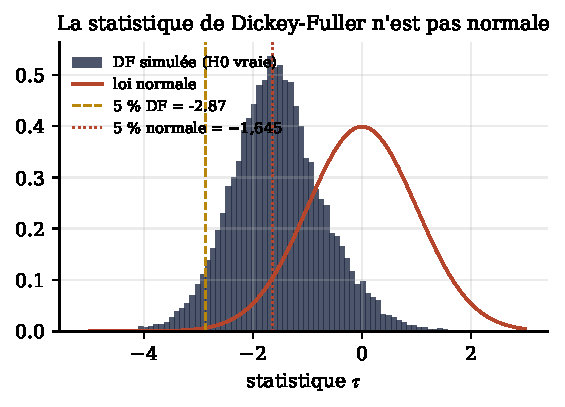
\includegraphics[width=0.6\textwidth]{ch03/dickey_fuller_distribution.pdf}
\caption{Distribution simulée de la statistique de Dickey-Fuller sous l'hypothèse de racine unitaire, comparée à la loi normale.}
\label{c3:fig:df}
\end{figure}

\subsection{Termes déterministes et valeurs critiques}

Les valeurs critiques dépendent de ce que l'on met dans la régression :

\begin{table}[h]
\centering\small
\caption{Valeurs critiques asymptotiques du test de Dickey-Fuller (statistique $\tau$).}
\label{c3:tab:crit}
\begin{tabular}{lccc}
\toprule
Régression & 1\,\% & 5\,\% & 10\,\% \\
\midrule
Sans constante : $\Delta x_t = \gamma x_{t-1} + \varepsilon_t$ & $-2{,}58$ & $-1{,}95$ & $-1{,}62$ \\
Avec constante : $\Delta x_t = c + \gamma x_{t-1} + \varepsilon_t$ & $-3{,}43$ & $-2{,}86$ & $-2{,}57$ \\
Avec constante et tendance : $\Delta x_t = c + \delta t + \gamma x_{t-1} + \varepsilon_t$ & $-3{,}96$ & $-3{,}41$ & $-3{,}13$ \\
\bottomrule
\end{tabular}
\end{table}

\paragraph{Lequel choisir ?} Pour un \emph{spread} de \emph{pairs trading} dont la moyenne n'est pas nulle, on met une constante. On ajoute une tendance seulement si une raison économique la justifie, comme un écart de frais de gestion entre deux ETF (section~\ref{c3:sec:cases}) ; ajouter une tendance \og au cas où\fg{} réduit la puissance.

\subsection{Le test augmenté (ADF)}

Si les chocs du \emph{spread} sont eux-mêmes autocorrélés, $\varepsilon_t$ n'est pas un bruit blanc et le test est faussé. Le test de Dickey-Fuller augmenté ajoute des retards de la variation :
\[
\Delta x_t = c + \gamma x_{t-1} + \sum_{j=1}^{p}\delta_j\,\Delta x_{t-j} + \varepsilon_t.
\]
Les retards absorbent l'autocorrélation de court terme ; les valeurs critiques asymptotiques restent celles du tableau~\ref{c3:tab:crit}. On choisit $p$ par un critère d'information (AIC ou BIC), ce que fait \texttt{statsmodels} avec \texttt{autolag="AIC"}.

% =====================================================================
\section{La puissance : combien de données faut-il ?}
% =====================================================================

La \emph{puissance} d'un test est la probabilité de rejeter $H_0$ quand elle est fausse. Ici : la probabilité de détecter un retour à la moyenne qui existe vraiment.

\begin{codebox}[ — E2, puissance du test ADF à 5\,\%]
\textbf{Protocole :} AR(1) stationnaires, 200 à 400 répétitions par case. \textbf{Résultats :} tableau~\ref{c3:tab:power} et figure~\ref{c3:fig:power}.
\end{codebox}

\begin{table}[h]
\centering\small
\caption{Probabilité que le test ADF (constante, 1 retard) rejette la racine unitaire à 5\,\%.}
\label{c3:tab:power}
\begin{tabular}{lccccc}
\toprule
 & $n = 100$ & $250$ & $500$ & $1\,000$ & $2\,500$ \\
\midrule
$\varphi = 0{,}90$ (demi-vie 6,6) & 29\,\% & 96\,\% & 100\,\% & 100\,\% & 100\,\% \\
$\varphi = 0{,}95$ (demi-vie 13,5) & 11\,\% & 44\,\% & 96\,\% & 100\,\% & 100\,\% \\
$\varphi = 0{,}98$ (demi-vie 34,3) & 9\,\% & 13\,\% & 33\,\% & 85\,\% & 100\,\% \\
$\varphi = 0{,}99$ (demi-vie 69,0) & 7\,\% & 6\,\% & 10\,\% & 32\,\% & 97\,\% \\
\bottomrule
\end{tabular}
\end{table}

\begin{figure}[h]
\centering
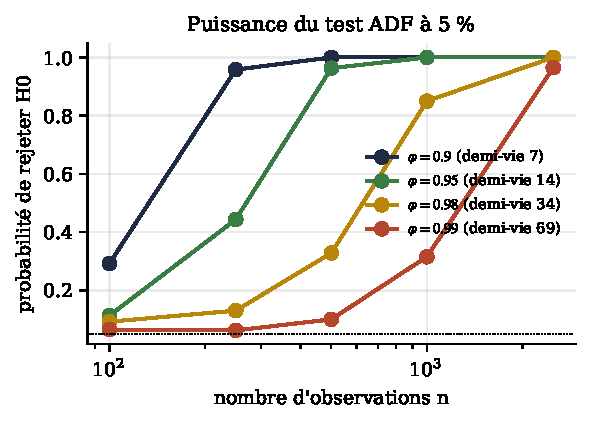
\includegraphics[width=0.6\textwidth]{ch03/puissance_adf.pdf}
\caption{Puissance du test ADF en fonction de la taille d'échantillon, pour quatre vitesses de retour.}
\label{c3:fig:power}
\end{figure}

\paragraph{La règle des demi-vies.} Les cases de puissance comparable ont un point commun : la quantité $n(1-\varphi)$. Avec $n(1-\varphi) = 10$ ($\varphi = 0{,}90$, $n = 100$ ; ou $\varphi = 0{,}99$, $n = 1\,000$), la puissance est d'environ 30\,\% ; avec $n(1-\varphi) = 25$ ($\varphi = 0{,}95$, $n=500$ ; ou $\varphi = 0{,}99$, $n = 2\,500$), elle dépasse 95\,\%. Or, d'après la proposition~\ref{c1:prop:hl}, $n(1-\varphi) \approx \ln 2 \times n/h_{1/2}$ : ce qui compte n'est pas le nombre de points, mais le \emph{nombre de demi-vies observées}. Règle pratique : il faut observer au moins une trentaine de demi-vies pour détecter un retour à la moyenne de façon fiable.

\begin{pitfall}
Passer de données quotidiennes à des données minute multiplie le nombre de points mais pas le nombre de demi-vies : si l'écart revient en 30 jours, une année de données minute contient toujours une douzaine de demi-vies, et le test reste peu puissant. Augmenter la fréquence n'aide que si la dynamique de retour est elle-même rapide.
\end{pitfall}

% =====================================================================
\section{Le test KPSS : inverser l'hypothèse nulle}
% =====================================================================

Le test ADF a pour hypothèse nulle la non-stationnarité ; ne pas la rejeter ne prouve pas qu'elle est vraie (manque de puissance). \citet{kpss1992} proposent l'inverse : $H_0$ = stationnarité. Le modèle est $x_t = \xi t + r_t + u_t$, où $r_t$ est une marche aléatoire de variance d'innovation $\sigma_r^2$ et $u_t$ est stationnaire ; $H_0 : \sigma_r^2 = 0$.

La statistique repose sur les sommes partielles des résidus $e_t$ de la régression de $x_t$ sur une constante (ou une constante et une tendance) : $S_t = \sum_{i\le t} e_i$, et
\[
\eta = \frac{1}{n^2}\,\frac{\sum_{t=1}^n S_t^2}{\hat\sigma^2_{LR}},
\]
où $\hat\sigma^2_{LR}$ est une variance de long terme estimée à la Newey-West (chapitre~2). Valeur critique à 5\,\% : $0{,}463$ (constante), $0{,}146$ (constante et tendance).

\begin{intuition}
Les écarts d'une série stationnaire s'annulent en moyenne : leur somme cumulée oscille autour de zéro, comme les dépenses et recettes d'un ménage bien géré. Ceux d'une série non stationnaire s'accumulent : la somme cumulée part au loin, comme une dette qui grossit. KPSS mesure la taille de cette somme cumulée.
\end{intuition}

\begin{codebox}[ — E3, combiner ADF et KPSS]
\textbf{Protocole :} 400 séries de 500 points par processus ; tests à 5\,\%. \textbf{Résultats :} marche aléatoire : ADF n'est pas rejeté et KPSS est rejeté dans 89\,\% des cas (conclusion correcte \og non stationnaire\fg). AR(1) avec $\varphi = 0{,}5$ : ADF rejeté, KPSS non rejeté dans 94\,\% des cas (conclusion correcte \og stationnaire\fg). AR(1) avec $\varphi = 0{,}95$ : les deux tests rejettent dans 40\,\% des cas, signe que la série est stationnaire mais très persistante.
\end{codebox}

\begin{table}[h]
\centering\small
\caption{Lecture conjointe des tests ADF et KPSS.}
\label{c3:tab:decision}
\begin{tabular}{lll}
\toprule
 & KPSS non rejeté & KPSS rejeté \\
\midrule
ADF rejeté & stationnaire (signal clair) & persistante, à confirmer \\
ADF non rejeté & données insuffisantes & non stationnaire (signal clair) \\
\bottomrule
\end{tabular}
\end{table}

% =====================================================================
\section{Le ratio de variance}
% =====================================================================

\subsection{Définition et calcul pour l'AR(1)}

Le ratio de variance compare la variance des variations sur $q$ périodes à $q$ fois la variance des variations sur une période :
\[
VR(q) = \frac{\Var(x_{t+q} - x_t)}{q\,\Var(x_{t+1}-x_t)}.
\]
Pour une marche aléatoire, $\Var(x_{t+q}-x_t) = q\sigma^2$ (proposition~\ref{c1:prop:rw}), donc $VR(q) = 1$.

\begin{proposition}\label{c3:prop:vr}
Pour un AR(1) stationnaire, $VR(q) = \dfrac{1-\varphi^q}{q\,(1-\varphi)}$, qui est strictement inférieur à 1 pour $0<\varphi<1$ et $q\ge2$.
\end{proposition}
\begin{proof}
Par la proposition~\ref{c1:prop:varspread} avec $\beta = 1$ et la proposition~\ref{c1:prop:ar1} : $\Var(x_{t+q}-x_t) = \gamma(0) + \gamma(0) - 2\gamma(q) = 2\gamma(0)(1-\varphi^q)$. De même, $\Var(x_{t+1}-x_t) = 2\gamma(0)(1-\varphi)$. Le rapport donne la formule. Comme $1-\varphi^q = (1-\varphi)(1+\varphi+\dots+\varphi^{q-1})$ et que chaque $\varphi^j < 1$ pour $j \ge 1$, on a $1-\varphi^q < q(1-\varphi)$.
\end{proof}

\begin{intuition}
Pour une marche aléatoire, les mouvements s'additionnent : dix jours bougent $\sqrt{10}$ fois plus qu'un jour. Pour un processus qui revient à la moyenne, les mouvements se compensent : dix jours bougent moins que ce que l'addition prédirait, $VR < 1$. Pour un processus qui suit une tendance, ils se renforcent : $VR > 1$.
\end{intuition}

\citet{lomackinlay1988} en déduisent un test : sous l'hypothèse de marche aléatoire à chocs homoscédastiques,
\[
z(q) = \frac{VR(q) - 1}{\sqrt{2(2q-1)(q-1)/(3qn)}}
\]
suit approximativement une loi $\N(0,1)$.

\begin{codebox}[ — E4, ratio de variance]
\textbf{Protocole :} séries de 5\,000 points. \textbf{Résultats :} pour l'AR(1) avec $\varphi = 0{,}9$, $VR(q)$ simulé vaut $0{,}954$ ; $0{,}823$ ; $0{,}655$ ; $0{,}417$ ; $0{,}224$ ; $0{,}150$ pour $q = 2, 5, 10, 20, 40, 60$, contre $0{,}950$ ; $0{,}819$ ; $0{,}651$ ; $0{,}439$ ; $0{,}246$ ; $0{,}166$ en théorie. Pour une série dont les rendements sont autocorrélés positivement (coefficient 0,3), $VR(10) = 1{,}77$. Statistique $z(10)$ : $-1{,}25$ (marche aléatoire, non significatif), $-7{,}21$ (AR), $+16{,}0$ (rendements autocorrélés). Pour la marche aléatoire, $VR(60) = 0{,}73$ : l'erreur-type de $VR(60)$ vaut environ $0{,}125$ ici, c'est un écart de deux erreurs-types dû au hasard, rappel que les grands horizons sont mal mesurés.
\end{codebox}

\begin{figure}[h]
\centering
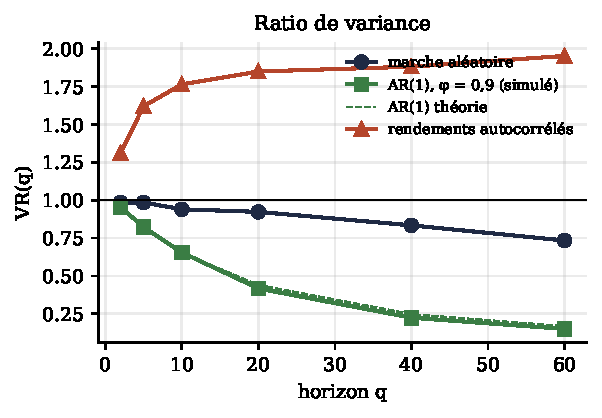
\includegraphics[width=0.6\textwidth]{ch03/ratio_variance.pdf}
\caption{Ratio de variance en fonction de l'horizon pour trois dynamiques.}
\label{c3:fig:vr}
\end{figure}

% =====================================================================
\section{L'exposant de Hurst}
% =====================================================================

L'exposant de Hurst $H$ résume la façon dont l'amplitude des variations croît avec l'horizon : $\mathrm{sd}(x_{t+\tau} - x_t) \propto \tau^H$. On l'estime par la pente de la régression de $\log\mathrm{sd}(x_{t+\tau}-x_t)$ sur $\log\tau$. Pour une marche aléatoire, $H = 1/2$ ; $H < 1/2$ indique un retour à la moyenne ; $H > 1/2$ une persistance des tendances \citep{chan2013}.

\begin{codebox}[ — E5, exposant de Hurst (retards 2 à 50)]
\textbf{Protocole :} 200 séries de 2\,000 points. \textbf{Résultats} (moyenne, et intervalle 5–95\,\%) : marche aléatoire $0{,}494$ $[0{,}44\,;\,0{,}55]$ ; AR(1) $\varphi=0{,}9$ : $0{,}218$ $[0{,}19\,;\,0{,}26]$ ; AR(1) $\varphi=0{,}99$ : $0{,}457$ $[0{,}40\,;\,0{,}51]$ ; rendements autocorrélés : $0{,}525$ $[0{,}47\,;\,0{,}58]$.
\end{codebox}

\begin{pitfall}
L'exposant de Hurst n'est pas une propriété intrinsèque : il dépend de la plage de retards choisie. Sur les retards 2 à 50, un AR(1) de demi-vie 69 jours ($\varphi = 0{,}99$) a un $H$ indiscernable de celui d'une marche aléatoire : le retour à la moyenne ne se manifeste qu'au-delà de la demi-vie. C'est le même problème de puissance que pour ADF, sous un autre nom. Utilisez Hurst et le ratio de variance comme diagnostics descriptifs, jamais comme tests uniques.
\end{pitfall}

% =====================================================================
\section{Études de cas réelles}\label{c3:sec:cases}
% =====================================================================

On applique les outils à deux écarts construits sur 500 séances réelles (octobre 2024 à octobre 2026).

\begin{table}[h]
\centering\small
\caption{Diagnostics de stationnarité sur données réelles (E6). ADF avec AIC ; KPSS avec retards automatiques ; $p$-valeurs KPSS bornées entre 0,01 et 0,10 par la table.}
\label{c3:tab:cases}
\begin{tabular}{lcccccc}
\toprule
Série & ADF $p$ & KPSS $p$ & $\hat\varphi$ & demi-vie (j) & $VR(10)$ & $H$ \\
\midrule
$\log$ GLD (un prix seul) & 0,547 & 0,01 & 0,9949 & 136,6 & 0,79 & 0,46 \\
$\log$ GLD $-$ $\log$ GLDM, constante seule & 0,925 & 0,01 & 0,9338 & 10,1 & 0,10 & 0,01 \\
idem, tests avec tendance & $<$0,001 & $\ge$0,10 & — & — & — & — \\
idem, tendance retirée & $<$0,001 & $\ge$0,10 & 0,0111 & 0,2 & 0,10 & 0,01 \\
$\log$ KO $-$ $\log$ PEP & 0,949 & 0,01 & 0,9996 & 1\,803 & 0,96 & 0,50 \\
$\log$ KO $-$ ($-0{,}432$) $\log$ PEP (MCO) & 0,684 & 0,01 & 0,9915 & 81,4 & 0,82 & 0,44 \\
\bottomrule
\end{tabular}
\end{table}

\begin{figure}[h]
\centering
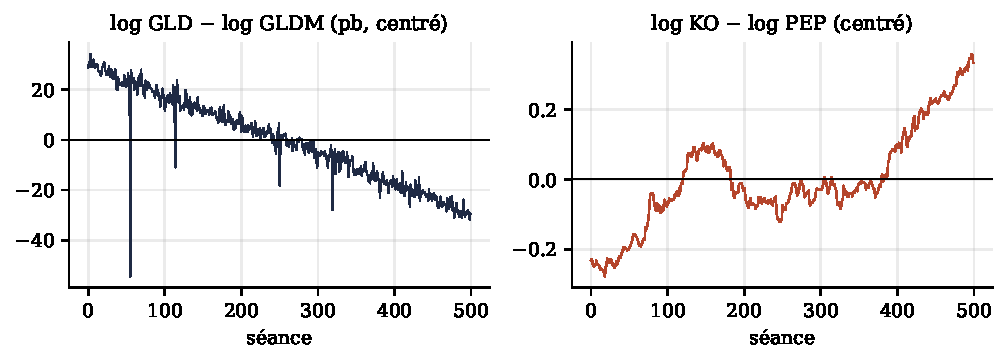
\includegraphics[width=0.95\textwidth]{ch03/cas_reels_ecarts.pdf}
\caption{À gauche, l'écart logarithmique entre GLD et GLDM en points de base : une pente régulière vers le bas plus un bruit quotidien de quelques points de base. À droite, l'écart logarithmique entre KO et PEP : une dérive sans retour.}
\label{c3:fig:cases}
\end{figure}

\paragraph{GLD et GLDM : un quasi-arbitrage parfaitement arbitré.} Les deux fonds détiennent de l'or physique. Avec une constante seule, ADF ne rejette pas la racine unitaire ($p = 0{,}925$) et KPSS rejette la stationnarité : conclusion naïve, \og non stationnaire\fg. C'est faux. Le log-ratio décroît régulièrement de $0{,}293\,\%$ par an : c'est l'ordre de grandeur de l'écart entre les frais de gestion annuels des deux fonds, prélevés jour après jour sur l'actif du fonds le plus cher. Avec une tendance dans la régression, ADF rejette massivement ($\tau = -22$) et KPSS ne rejette plus. Une fois la tendance retirée, l'écart a un écart-type de $4{,}5$ points de base, son quantile à 99\,\% vaut $8{,}3$ points de base, et $\hat\varphi = 0{,}011$ : un écart d'un jour a disparu le lendemain. Les participants autorisés, qui créent et détruisent des parts contre de l'or, maintiennent la relation. \textbf{Leçon :} il n'y a rien à gagner à l'échelle quotidienne après coûts ; s'il existe un avantage, il est intrajournalier et réservé à ceux qui exécutent vite et pour presque rien.

\paragraph{KO et PEP : la paire des manuels ne l'était pas.} Avec un ratio de 1 ou avec le ratio MCO (négatif, ce qui n'a aucun sens économique pour deux concurrents), l'écart ne montre aucun retour à la moyenne détectable. Le $\hat\varphi$ de $0{,}9915$ correspondrait à une demi-vie de 81 jours, soit à peine six demi-vies dans l'échantillon : le tableau~\ref{c3:tab:power} dit que, même si ce retour existait, on ne pourrait pas le détecter avec deux ans de données. Ajoutons que tester les résidus d'une régression estimée exige d'autres valeurs critiques (chapitre~4) : les $p$-valeurs de la dernière ligne sont même trop optimistes.

\section{Tests multiples : un avertissement}

Supposons que l'on teste 500 écarts candidats au seuil de 5\,\%. Même si aucun ne revient à la moyenne, on en déclarera en moyenne 25 \og stationnaires\fg. Les vrais retours à la moyenne, s'il y en a, sont noyés parmi les faux positifs, et ce sont souvent les faux positifs qui ont les meilleures statistiques en échantillon. Le chapitre~7 traite cette question (contrôle du taux de fausses découvertes) et le chapitre~16 en tire les conséquences pour l'évaluation des stratégies.

% =====================================================================
\section{Ce que la théorie apporte, et ses limites}
% =====================================================================

\paragraph{Apports.} Des valeurs critiques correctes, qui évitent de voir du retour à la moyenne partout ; un lien quantitatif entre durée d'observation et capacité de détection ; des diagnostics complémentaires (KPSS, ratio de variance, Hurst) qui, ensemble, donnent une image plus fiable qu'un test isolé.

\paragraph{Limites.} (1) Tous ces tests supposent des paramètres constants sur l'échantillon ; une rupture (changement de moyenne) fait ressembler une série stationnaire à une marche aléatoire. (2) Les tendances déterministes doivent être justifiées économiquement, sinon on teste ce qu'on veut voir. (3) Un test répond à une question statistique (\og y a-t-il une force de rappel ?\fg) ; la question économique (\og cette force est-elle assez rapide et ample pour payer les coûts ?\fg) demande une analyse séparée, comme le montre l'écart GLD/GLDM, parfaitement stationnaire et pourtant inexploitable.

% =====================================================================
\section{Fiche à recopier au tableau blanc}
% =====================================================================

\begin{whiteboard}
\begin{itemize}[leftmargin=1.2em]
\item \textbf{DF :} $\Delta x_t = c + \gamma x_{t-1} + \varepsilon_t$, $H_0 : \gamma = 0$ (racine unitaire), $\tau = \hat\gamma/\mathrm{se}$.
\item \textbf{Pourquoi non normale :} $\sum x_{t-1}\varepsilon_t = \frac12(x_n^2 - \sum\varepsilon_t^2)$ $\Rightarrow$ $\frac12(W^2-1)$, négatif 68\,\% du temps.
\item \textbf{Seuils 5\,\% :} $-1{,}95$ (rien), $-2{,}86$ (constante), $-3{,}41$ (tendance).
\item \textbf{ADF :} ajouter $\sum\delta_j\Delta x_{t-j}$, choisir $p$ par AIC.
\item \textbf{Puissance :} gouvernée par $n(1-\varphi)\approx 0{,}69\,n/h_{1/2}$ ; viser $\ge 30$ demi-vies.
\item \textbf{KPSS :} $H_0$ stationnarité ; $\eta = n^{-2}\sum S_t^2/\hat\sigma^2_{LR}$ ; seuil $0{,}463$.
\item \textbf{Ratio de variance :} $VR(q) = \Var(x_{t+q}-x_t)/(q\Var(\Delta x))$ ; AR(1) : $(1-\varphi^q)/(q(1-\varphi))$.
\item \textbf{Hurst :} $\mathrm{sd}(x_{t+\tau}-x_t)\propto\tau^H$ ; $H<\frac12$ retour, $=\frac12$ marche, $>\frac12$ tendance.
\end{itemize}
\end{whiteboard}

% =====================================================================
\section{Exercices}
% =====================================================================

\begin{exercise}
Refaites la démonstration de $\sum x_{t-1}\varepsilon_t = \frac12(x_n^2 - x_0^2 - \sum\varepsilon_t^2)$ avec $x_0 \ne 0$. Calculez $\Prob(W^2 < 1)$ à l'aide de la table de la loi normale.
\end{exercise}

\begin{exercise}
Un écart a une demi-vie estimée de 20 jours. Combien d'années de données quotidiennes faut-il pour avoir une puissance d'environ 95\,\% d'après la règle des demi-vies ? Et une demi-vie de 5 jours ?
\end{exercise}

\begin{exercise}
Calculez la limite de $VR(q)$ quand $q\to\infty$ pour un AR(1) stationnaire. Interprétez.
\end{exercise}

\begin{exercise}[à coder]
Simulez un AR(1) avec $\varphi = 0{,}8$ dont la moyenne saute de 0 à 5 au milieu de l'échantillon. Appliquez ADF et KPSS. Que concluez-vous à tort ? Comment détecter la rupture (voir chapitre~17) ?
\end{exercise}

\begin{exercise}[à coder]
Sur l'écart GLD/GLDM sans tendance, calculez l'autocorrélation des variations quotidiennes. Pourquoi est-elle proche de $-0{,}5$ quand l'écart est un bruit blanc ? (Indice : $\Var(\Delta x)$ et $\Cov(\Delta x_t,\Delta x_{t-1})$ pour un bruit blanc.)
\end{exercise}

% =====================================================================
\section{Pour aller plus loin}
% =====================================================================

\begin{toread}
\begin{itemize}[leftmargin=1.2em]
\item \citet{hamilton1994}, chapitre~17 (\og Univariate Processes with Unit Roots\fg) : la théorie asymptotique complète de Dickey-Fuller, avec les tables de valeurs critiques.
\item \citet{dickeyfuller1979} et \citet{kpss1992} : les articles originaux.
\item \citet{lomackinlay1988} : le test du ratio de variance, appliqué aux indices boursiers américains.
\item \citet{chan2013}, chapitre~2 : ADF, Hurst et ratio de variance appliqués à des paires réelles, avec code.
\end{itemize}
\end{toread}

\section{Scripts du chapitre}
\noindent\texttt{code/ch03/ch03\_stationarity\_tests.py} : E1 (figure~\ref{c3:fig:df}), E2 (tableau~\ref{c3:tab:power}, figure~\ref{c3:fig:power}), E3 (tableau~\ref{c3:tab:decision}), E4 (figure~\ref{c3:fig:vr}), E5 (Hurst), E6 (tableau~\ref{c3:tab:cases}, figure~\ref{c3:fig:cases}).

% =====================================================================
\chapter{Cointégration}
\label{ch:4}
% =====================================================================

\section{Objectifs et organisation du chapitre}

\paragraph{Objectifs.} Le chapitre~1 a donné l'intuition de la cointégration ; ce chapitre en donne la théorie et les outils. À la fin, vous saurez : (1) définir l'ordre d'intégration et la cointégration ; (2) appliquer la méthode d'Engle-Granger avec les bonnes valeurs critiques ; (3) expliquer la superconvergence du ratio de couverture et ses limites ; (4) écrire un modèle à correction d'erreur et en déduire qui \og corrige\fg{} l'écart et à quelle vitesse ; (5) comprendre la procédure de Johansen pour plusieurs actifs ; (6) reconnaître une cointégration partielle ; (7) appliquer le tout aux paires réelles du cours.

\paragraph{Code.} \texttt{code/ch04/ch04\_cointegration.py}, expériences E1 à E6.

% =====================================================================
\section{Ordre d'intégration et définition}
% =====================================================================

\begin{definition}[Ordre d'intégration]
Une série $x_t$ est \emph{intégrée d'ordre $d$}, notée $x_t\sim I(d)$, s'il faut la différencier $d$ fois pour obtenir une série stationnaire (sans tendance déterministe non modélisée). Une série stationnaire est $I(0)$ ; une marche aléatoire est $I(1)$, puisque $\Delta x_t = \varepsilon_t$ est $I(0)$.
\end{definition}

\begin{definition}[Cointégration, \citet{englegranger1987}]
Les composantes d'un vecteur $x_t = (x_{1t},\dots,x_{kt})^\top$, toutes $I(1)$, sont \emph{cointégrées} s'il existe un vecteur non nul $\beta\in\R^k$ tel que $\beta^\top x_t$ soit $I(0)$. Le vecteur $\beta$ est un \emph{vecteur de cointégration} ; le nombre $r$ de vecteurs linéairement indépendants qui ont cette propriété est le \emph{rang de cointégration}, avec $0\le r < k$.
\end{definition}

Pour deux actifs, $r$ vaut 0 (pas de relation) ou 1 (une relation), et le vecteur est défini à un facteur près ; on le \emph{normalise} en fixant le coefficient d'un actif à 1 : $\beta = (1, -\beta_2)$, d'où l'écart $S_t = x_{1t} - \beta_2x_{2t}$.

\begin{intuition}
Pensez à $k$ bateaux sur une mer agitée. La marée (une tendance stochastique commune) les soulève tous. S'il y a $k$ bateaux mais seulement $k-r$ marées indépendantes, il existe $r$ combinaisons de leurs hauteurs dans lesquelles les marées s'annulent : ce sont les écarts stationnaires. Deux bateaux sur la même marée : une combinaison. Deux bateaux dans deux ports différents : aucune.
\end{intuition}

% =====================================================================
\section{La méthode d'Engle-Granger}
% =====================================================================

\subsection{Les deux étapes}

\begin{enumerate}
\item \textbf{Estimer} la relation de long terme par MCO : $x_{1t} = a + b\,x_{2t} + e_t$ (chapitre~2).
\item \textbf{Tester} la stationnarité des résidus $\hat e_t$ par un test de Dickey-Fuller augmenté (chapitre~3), \emph{avec des valeurs critiques spécifiques}.
\end{enumerate}

\subsection{Pourquoi des valeurs critiques spécifiques}

À la première étape, les MCO choisissent $b$ pour que les résidus soient \emph{les plus petits possible}. Même si $x_1$ et $x_2$ ne sont pas cointégrés, ces résidus ont donc l'air \og plus stationnaires\fg{} qu'une marche aléatoire quelconque : la régression a déjà fait une partie du travail du test. Il faut donc des seuils plus exigeants. Avec deux variables et une constante, les valeurs asymptotiques de \citet{englegranger1987}, affinées par MacKinnon, sont $-3{,}90$ (1\,\%), $-3{,}34$ (5\,\%) et $-3{,}04$ (10\,\%) ; avec trois variables, $-4{,}29$ ; $-3{,}74$ ; $-3{,}45$.

\begin{codebox}[ — E1, valeurs critiques d'Engle-Granger]
\textbf{Protocole :} 10\,000 paires de marches aléatoires indépendantes de 500 points ; régression puis Dickey-Fuller sur les résidus. \textbf{Résultats :} quantiles simulés $-3{,}91$ ; $-3{,}36$ ; $-3{,}07$, conformes aux valeurs tabulées. Avec le seuil de Dickey-Fuller ($-2{,}86$), on déclarerait cointégrées $14{,}9\,\%$ des paires indépendantes, trois fois le taux nominal ; avec le seuil d'Engle-Granger, $5{,}3\,\%$.
\end{codebox}

\begin{figure}[h]
\centering
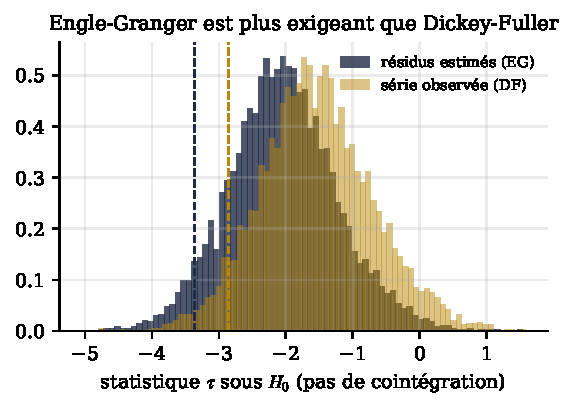
\includegraphics[width=0.62\textwidth]{ch04/eg_distribution.pdf}
\caption{Sous l'hypothèse d'absence de cointégration, la statistique calculée sur des résidus estimés (Engle-Granger) est décalée vers la gauche par rapport à celle d'une série observée (Dickey-Fuller).}
\label{c4:fig:eg}
\end{figure}

\subsection{La superconvergence du ratio}

Quand la paire est réellement cointégrée, l'estimateur MCO de $b$ converge vers la vraie valeur à la vitesse $1/n$, et non $1/\sqrt n$ comme dans une régression ordinaire : on parle de \emph{superconvergence}. L'intuition : le régresseur $x_2$ erre de plus en plus loin (sa variance empirique croît comme $n$), ce qui rend toute erreur sur $b$ de plus en plus coûteuse en somme des carrés.

\begin{codebox}[ — E2, superconvergence]
\textbf{Protocole :} vrai $b = 1{,}5$, écart AR(1) avec $\varphi = 0{,}9$, 500 répétitions. \textbf{Résultats :} écart-type de $\hat b$ : $0{,}111$ ($n = 250$), $0{,}030$ ($n = 1\,000$), $0{,}0081$ ($n = 4\,000$) ; il est divisé par environ 4 quand $n$ est multiplié par 4 (vitesse $1/n$). Pour une régression entre variables stationnaires : $0{,}067$ ; $0{,}030$ ; $0{,}016$, divisé par 2 seulement (vitesse $1/\sqrt n$).
\end{codebox}

\begin{pitfall}
La superconvergence est un résultat asymptotique qui suppose que la tendance commune domine le bruit de l'écart. Sur deux ans de données, avec un écart volatil, $\hat b$ peut rester loin de la vérité (voir E3 ci-dessous, où $\hat b = 0{,}88$ pour une vraie valeur de 1). Elle ne protège en rien contre une relation qui change au cours du temps.
\end{pitfall}

% =====================================================================
\section{Le modèle à correction d'erreur}
% =====================================================================

\subsection{Le théorème de représentation de Granger}

\begin{theorem}[Représentation de Granger, énoncé simplifié]
Deux séries $I(1)$ sont cointégrées, d'écart $S_t = x_{1t} - \beta x_{2t}$, si et seulement si elles admettent une représentation à correction d'erreur
\begin{align*}
\Delta x_{1t} &= \mu_1 + \alpha_1 S_{t-1} + \text{(retards de } \Delta x_1, \Delta x_2) + \varepsilon_{1t},\\
\Delta x_{2t} &= \mu_2 + \alpha_2 S_{t-1} + \text{(retards de } \Delta x_1, \Delta x_2) + \varepsilon_{2t},
\end{align*}
avec $(\alpha_1,\alpha_2)\ne(0,0)$.
\end{theorem}

Les coefficients $\alpha_1$, $\alpha_2$ sont les \emph{vitesses d'ajustement}. Si l'écart est positif ($x_1$ trop haut par rapport à $x_2$), il faut que $x_1$ baisse ($\alpha_1<0$) ou que $x_2$ monte ($\alpha_2>0$), ou les deux.

\begin{intuition}
Dans l'image de \citet{murray1994}, si la promeneuse appelle son chien et que le chien revient, c'est le chien qui \og corrige l'erreur\fg{} ; si la promeneuse va chercher son chien, c'est elle ; souvent, les deux font la moitié du chemin. Le modèle à correction d'erreur mesure qui fait quoi.
\end{intuition}

\subsection{Vitesse de retour de l'écart}

\begin{proposition}\label{c4:prop:ecm}
Sans retards, l'écart suit $\Delta S_t = (\mu_1 - \beta\mu_2) + (\alpha_1 - \beta\alpha_2)\,S_{t-1} + (\varepsilon_{1t} - \beta\varepsilon_{2t})$. C'est un AR(1) de coefficient $\varphi_S = 1 + \alpha_1 - \beta\alpha_2$.
\end{proposition}
\begin{proof}
$\Delta S_t = \Delta x_{1t} - \beta\Delta x_{2t}$ ; on remplace chaque variation par son équation et on regroupe les termes en $S_{t-1}$. On reconnaît l'écriture \og retour à la moyenne\fg{} de l'AR(1), équation~\eqref{c1:eq:ecm} du chapitre~1, avec $\varphi_S - 1 = \alpha_1 - \beta\alpha_2$.
\end{proof}

\begin{codebox}[ — E3, correction d'erreur]
\textbf{Protocole :} système simulé ($n = 2\,000$) avec $\beta = 1$, $\alpha_1 = -0{,}10$, $\alpha_2 = +0{,}05$ ; donc $\varphi_S = 1 - 0{,}10 - 0{,}05 = 0{,}85$ et une demi-vie de $4{,}27$ jours. \textbf{Résultats :} $\hat\beta = 0{,}879$ ; $\hat\alpha_1 = -0{,}127$ ($t = -13{,}3$) ; $\hat\alpha_2 = 0{,}055$ ($t = 6{,}0$) ; $\hat\varphi_S = 0{,}825$, demi-vie $3{,}6$ jours. Les deux jambes participent à la correction, avec les bons signes. Le biais sur $\beta$ vient de ce que, dans ce système, la tendance commune est faible par rapport au bruit de l'écart.
\end{codebox}

\paragraph{Lecture pour le trading.} Si seule une jambe corrige ($\alpha_2 \approx 0$), l'autre est le \og meneur\fg{} : c'est elle qui porte l'information, et c'est sur la jambe suiveuse que le retour se produit. Pour un \emph{pairs trade}, cela influence le choix de la jambe à exécuter en premier et le risque d'exécution (chapitre~15). Dans le cas \texttt{atjte}, le CFD sur MT5 sert de prix de référence : on suppose implicitement que c'est le prix sur la plateforme crypto qui s'ajuste.

% =====================================================================
\section{Plusieurs actifs : la procédure de Johansen}
% =====================================================================

\subsection{Le VECM}

Avec $k$ actifs, on écrit un modèle vectoriel à correction d'erreur (VECM) :
\[
\Delta x_t = \mu + \Pi\,x_{t-1} + \sum_{i=1}^{p-1}\Gamma_i\,\Delta x_{t-i} + \varepsilon_t, \qquad \Pi = \alpha\beta^\top,
\]
où $\alpha$ et $\beta$ sont des matrices $k\times r$. Les colonnes de $\beta$ sont les vecteurs de cointégration, celles de $\alpha$ les vitesses d'ajustement. Le rang de $\Pi$ est le nombre de relations de cointégration : rang 0, pas de relation (le modèle se réduit à un VAR en différences) ; rang $k$, toutes les séries sont stationnaires ; entre les deux, $r$ relations.

\subsection{L'idée de Johansen}

\citet{johansen1991} estime le VECM par maximum de vraisemblance. Après avoir retiré l'effet des retards $\Delta x_{t-i}$ par régression, il calcule les \emph{corrélations canoniques} entre les variations $\Delta x_t$ et les niveaux $x_{t-1}$ : ce sont les combinaisons des niveaux qui prédisent le mieux les variations. Les carrés de ces corrélations sont des valeurs propres $\hat\lambda_1 \ge \dots \ge \hat\lambda_k$ ; un $\hat\lambda_i$ nettement positif signale une combinaison de niveaux qui \og rappelle\fg{} les prix, donc une relation de cointégration. Deux statistiques testent le rang :
\[
\text{trace}(r) = -T\sum_{i=r+1}^{k}\ln(1-\hat\lambda_i), \qquad \text{valeur propre max}(r) = -T\ln(1-\hat\lambda_{r+1}),
\]
qui testent $H_0$ : rang $\le r$. On teste successivement $r = 0, 1, \dots$ et on s'arrête au premier non-rejet.

\begin{codebox}[ — E4, Johansen sur trois actifs]
\textbf{Protocole :} $x_1$ et $x_2$ partagent une tendance commune ($x_2 = 0{,}5\times$ tendance $+$ AR(1)), $x_3$ suit sa propre tendance ; une seule relation, $x_2 - 0{,}5x_1$. \textbf{Résultats :} statistique de trace $48{,}1$ ; $6{,}1$ ; $2{,}1$ pour $r = 0, 1, 2$, contre des seuils à 5\,\% de $29{,}8$ ; $15{,}5$ ; $3{,}8$ : on rejette $r = 0$, pas $r = 1$ : rang 1, correct. Vecteur estimé normalisé sur $x_2$ : $(-0{,}535\,;\,1\,;\,-0{,}042)$, proche de $(-0{,}5\,;\,1\,;\,0)$.
\end{codebox}

\paragraph{Engle-Granger ou Johansen ?} Engle-Granger est simple et transparent mais dépend du choix de la variable normalisée et ne trouve qu'une relation ; Johansen traite les actifs symétriquement et estime le nombre de relations, mais il est sensible à la spécification (retards, termes déterministes) et ses propriétés sur petits échantillons sont moins bonnes. En \emph{pairs trading}, on utilise souvent Engle-Granger pour la sélection et Johansen pour les paniers de trois actifs et plus.

% =====================================================================
\section{La cointégration partielle}
% =====================================================================

Les paires réelles ne sont presque jamais parfaitement cointégrées : leur relation dérive lentement (changement de modèle économique, de structure de coûts). \citet{clegg2018} modélisent l'écart comme la somme de deux composantes cachées,
\[
S_t = M_t + R_t, \qquad M_t = \rho M_{t-1} + \varepsilon^M_t,\quad R_t = R_{t-1} + \varepsilon^R_t,
\]
une partie qui revient à la moyenne ($|\rho|<1$, écart-type d'innovation $\sigma_M$) et une partie marche aléatoire (écart-type $\sigma_R$). Comme $R$ est une marche aléatoire, $S$ n'est pas stationnaire : un test de cointégration classique conclut à l'absence de relation. Pourtant, une partie des variations de l'écart est prévisible.

\begin{proposition}\label{c4:prop:r2mr}
La part de la variance des variations de l'écart due à la composante de retour à la moyenne vaut
\[
R^2_{MR} = \frac{\Var(\Delta M_t)}{\Var(\Delta S_t)} = \frac{2\sigma_M^2}{2\sigma_M^2 + (1+\rho)\sigma_R^2}.
\]
\end{proposition}
\begin{proof}
D'après la démonstration de la proposition~\ref{c3:prop:vr} avec $q=1$, $\Var(\Delta M_t) = 2\gamma_M(0)(1-\rho) = 2\frac{\sigma_M^2}{1-\rho^2}(1-\rho) = \frac{2\sigma_M^2}{1+\rho}$. Par ailleurs $\Var(\Delta R_t) = \sigma_R^2$, et les deux composantes sont indépendantes, donc $\Var(\Delta S_t) = \frac{2\sigma_M^2}{1+\rho} + \sigma_R^2$. On fait le rapport et on multiplie numérateur et dénominateur par $1+\rho$.
\end{proof}

\begin{codebox}[ — E5, ADF face à la cointégration partielle]
\textbf{Protocole :} $\rho = 0{,}9$, $\sigma_M = 1$, $n = 1\,000$, 300 répétitions. \textbf{Résultats :} pour $\sigma_R = 0$ ; $0{,}1$ ; $0{,}2$ ; $0{,}4$ ; $0{,}8$, on a $R^2_{MR} = 1$ ; $0{,}991$ ; $0{,}963$ ; $0{,}868$ ; $0{,}622$ et le test ADF conclut à la stationnarité dans $100$ ; $98{,}7$ ; $86{,}7$ ; $53{,}3$ ; $17{,}7\,\%$ des cas. Une marche aléatoire qui ne représente que 13\,\% de la variance des variations suffit à rendre le test aveugle une fois sur deux.
\end{codebox}

L'estimation de $(\rho,\sigma_M,\sigma_R)$ se fait par filtre de Kalman, puisque $M$ et $R$ sont des états cachés : ce sera l'objet du chapitre~8.

% =====================================================================
\section{Études de cas réelles}
% =====================================================================

\begin{table}[h]
\centering\small
\caption{Tests de cointégration sur les log-prix (E6).}
\label{c4:tab:real}
\begin{tabular}{lccc}
\toprule
Test & Statistique & $p$-valeur & Seuil 5\,\% \\
\midrule
Engle-Granger, GLD sur GLDM, constante & $-0{,}53$ & 0,962 & $-3{,}35$ \\
Engle-Granger, GLD sur GLDM, tendance & $-22{,}17$ & $<0{,}001$ & $-3{,}80$ \\
Johansen GLD/GLDM avec tendance, trace $r=0$ & $214{,}4$ & — & $18{,}4$ \\
Engle-Granger, KO sur PEP & $-1{,}18$ & 0,864 & $-3{,}35$ \\
Engle-Granger, PEP sur KO & $-3{,}17$ & 0,075 & $-3{,}35$ \\
Johansen KO/PEP, trace $r=0$ & $9{,}99$ & — & $15{,}49$ \\
\bottomrule
\end{tabular}
\end{table}

\paragraph{GLD/GLDM.} Les conclusions du chapitre~3 se confirment : cointégration écrasante dès qu'on autorise la tendance due à l'écart de frais, aucune sinon. Johansen, avec un terme déterministe adapté, trouve aussi une relation.

\paragraph{KO/PEP.} Selon le sens de la régression, la $p$-valeur d'Engle-Granger passe de $0{,}864$ à $0{,}075$ : l'asymétrie du chapitre~2 se répercute sur le test. Johansen, symétrique, ne trouve pas de relation. Conclusion honnête : rien sur cette période ne justifie de traiter KO et PEP comme une paire cointégrée ; un trader qui aurait choisi le sens \og PEP sur KO\fg{} parce qu'il donne la meilleure $p$-valeur aurait fait, sans le savoir, deux tests et retenu le meilleur.

% =====================================================================
\section{Ce que la théorie apporte, et ses limites}
% =====================================================================

\paragraph{Apports.} La cointégration donne une justification statistique précise au \emph{pairs trading} : un écart stationnaire entre deux prix non stationnaires. Le modèle à correction d'erreur relie l'écart à la dynamique de chaque jambe et donne sa vitesse de retour ; Johansen étend le cadre aux paniers.

\paragraph{Limites.} (1) Les tests héritent du manque de puissance du chapitre~3 : sur deux ans, une relation réelle mais lente passe inaperçue. (2) La cointégration est une propriété \og pour toujours\fg{} ; les marchés offrent au mieux des relations temporaires, d'où l'intérêt de la cointégration partielle et des modèles à paramètres variables (chapitre~8). (3) Le choix du sens, des termes déterministes et des retards multiplie les tests implicites. (4) Une relation statistique sans raison économique (même secteur, même sous-jacent, contrainte contractuelle) a peu de chances de survivre hors échantillon.

% =====================================================================
\section{Fiche à recopier au tableau blanc}
% =====================================================================

\begin{whiteboard}
\begin{itemize}[leftmargin=1.2em]
\item \textbf{$I(d)$ :} différencier $d$ fois pour être stationnaire. Prix $\sim I(1)$.
\item \textbf{Cointégration :} $x\sim I(1)$, $\beta^\top x\sim I(0)$ ; rang $r$ = nombre de relations indépendantes.
\item \textbf{Engle-Granger :} MCO en niveaux, puis ADF sur résidus ; seuils 5\,\% : $-3{,}34$ (2 var.), $-3{,}74$ (3 var.).
\item \textbf{Superconvergence :} $\hat b - b = O(1/n)$ si la paire est cointégrée.
\item \textbf{Correction d'erreur :} $\Delta x_{1t} = \alpha_1S_{t-1}+\dots$, $\Delta x_{2t} = \alpha_2S_{t-1}+\dots$ ; $\varphi_S = 1+\alpha_1-\beta\alpha_2$.
\item \textbf{VECM :} $\Delta x_t = \Pi x_{t-1} + \sum\Gamma_i\Delta x_{t-i} + \varepsilon_t$, $\Pi = \alpha\beta^\top$, rang $r$.
\item \textbf{Johansen :} trace $= -T\sum_{i>r}\ln(1-\hat\lambda_i)$ ; tester $r = 0, 1, \dots$
\item \textbf{Cointégration partielle :} $S = M + R$ ; $R^2_{MR} = 2\sigma_M^2/(2\sigma_M^2 + (1+\rho)\sigma_R^2)$.
\end{itemize}
\end{whiteboard}

% =====================================================================
\section{Exercices}
% =====================================================================

\begin{exercise}
Montrez que si $x_t\sim I(1)$ et $y_t = 2x_t + u_t$ avec $u_t$ stationnaire, alors $y_t\sim I(1)$ et $(1,-2)$ est un vecteur de cointégration. Le vecteur $(2,-4)$ en est-il un aussi ?
\end{exercise}

\begin{exercise}
Dans un modèle à correction d'erreur avec $\beta = 1$, $\alpha_1 = -0{,}02$ et $\alpha_2 = 0$, calculez la demi-vie de l'écart. Quelle jambe faut-il surveiller pour anticiper la fermeture de l'écart ?
\end{exercise}

\begin{exercise}
Que se passe-t-il dans la proposition~\ref{c4:prop:ecm} si $\alpha_1 = \beta\alpha_2$ ? Interprétez.
\end{exercise}

\begin{exercise}
Avec $\rho = 0{,}8$ et $\sigma_M = 1$, quelle valeur de $\sigma_R$ donne $R^2_{MR} = 0{,}5$ ?
\end{exercise}

\begin{exercise}[à coder]
Écrivez votre propre fonction \texttt{engle\_granger(y, x)} qui renvoie $\hat b$, la statistique ADF des résidus et une décision au seuil $-3{,}34$, et comparez-la à \texttt{statsmodels.tsa.stattools.coint} sur E1 et E6.
\end{exercise}

\begin{exercise}[à coder]
Estimez le VECM complet de GLD/GLDM avec \texttt{statsmodels.tsa.vector\_ar.vecm.VECM}. Quelle jambe corrige l'écart ? Est-ce cohérent avec la liquidité relative des deux fonds ?
\end{exercise}

% =====================================================================
\section{Pour aller plus loin}
% =====================================================================

\begin{toread}
\begin{itemize}[leftmargin=1.2em]
\item \citet{englegranger1987} : définition, théorème de représentation et méthode en deux étapes.
\item \citet{johansen1991} : la procédure du maximum de vraisemblance ; \citet{hamilton1994}, chapitres~19 (\og Cointegration\fg) et~20 (\og Full-Information Maximum Likelihood Analysis of Cointegrated Systems\fg) pour une présentation pas à pas.
\item \citet{vidyamurthy2004} : la cointégration appliquée au \emph{pairs trading}, avec la notion de tendance commune.
\item \citet{clegg2018} : la cointégration partielle et son estimation.
\item \citet{chan2013}, chapitre~2 : Engle-Granger et Johansen sur des paires d'ETF, avec code.
\end{itemize}
\end{toread}

\section{Scripts du chapitre}
\noindent\texttt{code/ch04/ch04\_cointegration.py} : E1 (figure~\ref{c4:fig:eg}), E2 (superconvergence), E3 (correction d'erreur), E4 (Johansen), E5 (cointégration partielle), E6 (tableau~\ref{c4:tab:real}).

% =====================================================================
\chapter{Le processus d'Ornstein-Uhlenbeck}
\label{ch:5}
% =====================================================================

\section{Objectifs et organisation du chapitre}

\paragraph{Objectifs.} Le processus d'Ornstein-Uhlenbeck (OU) est la version en temps continu de l'AR(1). Il est devenu le modèle standard de l'écart en arbitrage statistique \citep{avellaneda2010,bertram2010,leungli2016}, parce qu'il permet de calculer explicitement des durées de détention et des seuils optimaux. À la fin du chapitre, vous saurez : (1) ce qu'est un mouvement brownien et une équation différentielle stochastique ; (2) appliquer le lemme d'Itô pour résoudre l'équation d'OU ; (3) passer exactement de l'OU à l'AR(1) et inversement, et estimer les paramètres ; (4) calculer le temps moyen de retour à la moyenne par l'équation de Kolmogorov ; (5) choisir des seuils d'entrée qui maximisent le gain par unité de temps en présence de coûts.

\paragraph{Code.} \texttt{code/ch05/ch05\_ornstein\_uhlenbeck.py}, expériences E1 à E5.

% =====================================================================
\section{Mouvement brownien et équations différentielles stochastiques}
% =====================================================================

\subsection{Le mouvement brownien}

\begin{definition}
Un mouvement brownien standard $(W_t)_{t\ge0}$ est un processus en temps continu tel que $W_0 = 0$, ses trajectoires sont continues, et pour $s<t$ l'accroissement $W_t - W_s$ suit une loi $\N(0, t-s)$, indépendante de tout ce qui s'est passé avant $s$.
\end{definition}

C'est la limite de la marche aléatoire du chapitre~1 quand on fait des pas de plus en plus petits et de plus en plus fréquents. Sur un petit intervalle $\dd t$, l'accroissement $\dd W_t$ est d'ordre $\sqrt{\dd t}$ (son écart-type), et non $\dd t$. Conséquence capitale : $(\dd W_t)^2$, d'espérance $\dd t$ et de variance $2\dd t^2$, se comporte comme la quantité déterministe $\dd t$ ; on écrit $(\dd W_t)^2 = \dd t$.

\subsection{Équation différentielle stochastique}

Une équation différentielle stochastique (EDS) décrit l'évolution infinitésimale d'un processus :
\[
\dd X_t = b(X_t)\,\dd t + s(X_t)\,\dd W_t,
\]
où $b$ est la \emph{dérive} (la tendance locale) et $s$ la \emph{volatilité}. On la lit comme la limite de $X_{t+\Delta} - X_t \approx b(X_t)\Delta + s(X_t)\sqrt\Delta\,Z$, avec $Z\sim\N(0,1)$.

\subsection{Le lemme d'Itô}

\begin{proposition}[Lemme d'Itô, forme simple]
Si $\dd X_t = b\,\dd t + s\,\dd W_t$ et si $f(t,x)$ est deux fois dérivable, alors
\[
\dd f(t, X_t) = \Big(\partial_t f + b\,\partial_x f + \tfrac12 s^2\,\partial_{xx}f\Big)\dd t + s\,\partial_x f\,\dd W_t.
\]
\end{proposition}
\begin{proof}[Idée de la démonstration]
On développe $f$ à l'ordre 2 : $\dd f = \partial_t f\,\dd t + \partial_x f\,\dd X + \frac12\partial_{xx}f\,(\dd X)^2 + \dots$ Or $(\dd X)^2 = b^2\dd t^2 + 2bs\,\dd t\,\dd W + s^2(\dd W)^2$ ; les deux premiers termes sont négligeables (d'ordre $\dd t^{3/2}$ ou plus) et le troisième vaut $s^2\dd t$. On remplace $\dd X$ par $b\,\dd t + s\,\dd W$ et on regroupe.
\end{proof}

Le terme $\frac12 s^2\partial_{xx}f$ n'existe pas en calcul ordinaire : il vient de ce que le hasard brownien a une variance d'ordre $\dd t$.

% =====================================================================
\section{Le processus d'Ornstein-Uhlenbeck}
% =====================================================================

\subsection{Définition et solution}

\begin{definition}[\citet{uhlenbeck1930}]
Le processus d'Ornstein-Uhlenbeck est la solution de
\[
\dd X_t = \theta(\mu - X_t)\,\dd t + \sigma\,\dd W_t, \qquad \theta>0,\ \sigma>0.
\]
\end{definition}

La dérive $\theta(\mu - X_t)$ tire le processus vers $\mu$ avec une force proportionnelle à l'écart : c'est l'élastique du chapitre~1, en temps continu. $\theta$ est la \emph{vitesse de retour}, $\mu$ le niveau d'équilibre, $\sigma$ la volatilité instantanée.

\begin{proposition}\label{c5:prop:sol}
La solution vaut
\[
X_t = \mu + (X_0-\mu)e^{-\theta t} + \sigma\int_0^t e^{-\theta(t-u)}\,\dd W_u,
\]
de sorte que, sachant $X_0$, $X_t$ suit une loi normale de moyenne $\mu + (X_0-\mu)e^{-\theta t}$ et de variance $\frac{\sigma^2}{2\theta}\big(1-e^{-2\theta t}\big)$.
\end{proposition}
\begin{proof}
On applique le lemme d'Itô à $f(t,x) = e^{\theta t}x$ : $\partial_t f = \theta e^{\theta t}x$, $\partial_x f = e^{\theta t}$, $\partial_{xx}f = 0$. Donc
\[
\dd(e^{\theta t}X_t) = \big(\theta e^{\theta t}X_t + \theta(\mu - X_t)e^{\theta t}\big)\dd t + \sigma e^{\theta t}\dd W_t = \theta\mu\,e^{\theta t}\dd t + \sigma e^{\theta t}\dd W_t.
\]
Les termes en $X_t$ se sont annulés. On intègre de 0 à $t$ : $e^{\theta t}X_t - X_0 = \mu(e^{\theta t} - 1) + \sigma\int_0^t e^{\theta u}\dd W_u$, puis on multiplie par $e^{-\theta t}$. L'intégrale stochastique a une espérance nulle ; sa variance vaut, par la propriété d'isométrie (la variance d'une intégrale brownienne est l'intégrale du carré de l'intégrande), $\sigma^2\int_0^t e^{-2\theta(t-u)}\dd u = \frac{\sigma^2}{2\theta}(1-e^{-2\theta t})$.
\end{proof}

\paragraph{Conséquences.} Quand $t\to\infty$, la loi de $X_t$ tend vers la loi stationnaire $\N\big(\mu, \sigma^2/(2\theta)\big)$. L'écart-type stationnaire $\sigma_{eq} = \sigma/\sqrt{2\theta}$ est l'unité naturelle pour placer les seuils de trading. L'écart espéré à la moyenne est divisé par deux en
\[
h_{1/2} = \frac{\ln 2}{\theta}.
\]

\begin{figure}[h]
\centering
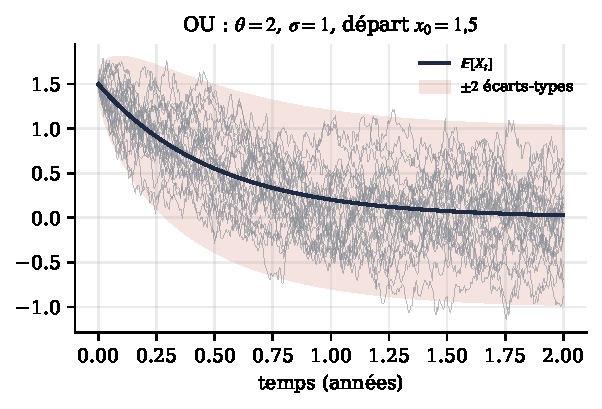
\includegraphics[width=0.62\textwidth]{ch05/ou_trajectoires.pdf}
\caption{Trajectoires d'un OU partant de $x_0 = 1{,}5$ : la moyenne décroît exponentiellement vers 0 et la dispersion converge vers $\pm2\sigma_{eq}$.}
\label{c5:fig:paths}
\end{figure}

\subsection{De l'OU à l'AR(1), exactement}

En observant le processus à intervalles réguliers $\Delta$ (un jour, $\Delta = 1/252$ an), la proposition~\ref{c5:prop:sol} appliquée entre $t$ et $t+\Delta$ donne exactement
\[
X_{t+\Delta} = \mu + e^{-\theta\Delta}(X_t - \mu) + \eta_t, \qquad \eta_t \sim \N\Big(0,\ \frac{\sigma^2}{2\theta}\big(1-e^{-2\theta\Delta}\big)\Big),
\]
c'est-à-dire un AR(1) avec
\[
\varphi = e^{-\theta\Delta}, \qquad \sigma_\eta^2 = \frac{\sigma^2}{2\theta}(1-\varphi^2).
\]
Inversement, une estimation $\hat\varphi$ de l'AR(1) donne $\hat\theta = -\ln\hat\varphi/\Delta$ et $\hat\sigma = \hat\sigma_\eta\sqrt{2\hat\theta/(1-\hat\varphi^2)}$. Le schéma d'Euler, $X_{t+\Delta} = X_t + \theta(\mu - X_t)\Delta + \sigma\sqrt\Delta Z$, n'est qu'une approximation : il remplace $e^{-\theta\Delta}$ par $1-\theta\Delta$.

\begin{codebox}[ — E1, discrétisation exacte contre Euler]
\textbf{Protocole :} $\theta = 2$ (demi-vie de $0{,}35$ an), $\sigma = 1$, variance stationnaire théorique $0{,}25$. \textbf{Résultats :} pas quotidien ($\Delta = 1/252$) : les deux schémas donnent une autocorrélation de $0{,}992$, identique à la théorie. Pas mensuel : exact $0{,}846$ (théorie $0{,}847$), Euler $0{,}830$ ; variance Euler $0{,}273$. Pas trimestriel : exact $0{,}610$ (théorie $0{,}607$), Euler $0{,}505$ ; variance Euler $0{,}324$, soit 30\,\% de trop. \textbf{Leçon :} simulez toujours avec la discrétisation exacte, qui est aussi simple à coder.
\end{codebox}

\subsection{Estimation}

\begin{codebox}[ — E2, estimation des paramètres]
\textbf{Protocole :} $\theta = 5$ (demi-vie de 35 jours), $\mu = 1$, $\sigma = 0{,}5$ ; 500 trajectoires quotidiennes par durée. \textbf{Résultats} (médiane et intervalle 5–95\,\% de $\hat\theta$) : 1 an : $8{,}65$ $[2{,}8\,;\,20{,}6]$ ; 4 ans : $5{,}81$ $[3{,}4\,;\,9{,}8]$ ; 16 ans : $5{,}22$ $[4{,}0\,;\,6{,}8]$. $\hat\sigma$ est très précis dès un an (médiane $0{,}504$), $\hat\mu$ l'est beaucoup moins (écart-type $0{,}12$ sur un an pour un écart-type stationnaire de $0{,}16$).
\end{codebox}

\begin{pitfall}
Sur un an, la vitesse de retour est surestimée de 70\,\% en médiane, ce qui divise la demi-vie apparente presque par deux : c'est le biais de Kendall du chapitre~2, traduit en temps continu. La moyenne $\mu$ est elle aussi mal connue, alors que tous les seuils de trading sont placés autour d'elle. La volatilité, elle, est bien estimée : c'est le paramètre le plus fiable et le moins important pour la décision.
\end{pitfall}

% =====================================================================
\section{Combien de temps pour revenir ? Les temps de premier passage}
% =====================================================================

\subsection{L'équation de Kolmogorov}

Notons $u(x)$ le temps moyen que met le processus, parti de $x$, pour atteindre un niveau cible. Pendant un court instant $\dd t$, il s'écoule $\dd t$ et le processus passe de $x$ à $x + \dd X$ ; ensuite, il reste en moyenne $u(x+\dd X)$ :
\[
u(x) = \dd t + \E\big[u(x + \dd X)\big].
\]
On développe $u$ à l'ordre 2 et l'on utilise $\E[\dd X] = b(x)\dd t$ et $\E[(\dd X)^2] = s(x)^2\dd t$ :
\[
u(x) = \dd t + u(x) + b(x)u'(x)\dd t + \tfrac12 s(x)^2u''(x)\dd t \quad\Longrightarrow\quad \tfrac12 s(x)^2u''(x) + b(x)u'(x) = -1.
\]
C'est l'équation de Kolmogorov rétrograde pour les temps moyens de sortie.

\subsection{Résolution pour l'OU}

Prenons $\mu = 0$ (on mesure l'écart à la moyenne), $b(x) = -\theta x$, $s = \sigma$, et posons $k = \theta/\sigma^2$, $v = u'$. L'équation devient $\frac{\sigma^2}{2}v' - \theta x\,v = -1$. En multipliant par le facteur intégrant $\frac{2}{\sigma^2}e^{-kx^2}$, le membre de gauche devient une dérivée exacte :
\[
\frac{\dd}{\dd x}\Big(v(x)\,e^{-kx^2}\Big) = -\frac{2}{\sigma^2}e^{-kx^2}.
\]

\begin{proposition}[Temps moyens de passage de l'OU]\label{c5:prop:fpt}
Avec $k = \theta/\sigma^2$ et un seuil $a>0$ :
\begin{align*}
\text{(retour)}\quad T_{a\to 0} &= \frac{2}{\sigma^2}\int_0^a e^{ky^2}\Big(\int_y^{\infty}e^{-kz^2}\dd z\Big)\dd y,\\
\text{(attente)}\quad T_{0\to\pm a} &= \frac{2}{\sigma^2}\int_0^a e^{ky^2}\Big(\int_0^{y}e^{-kz^2}\dd z\Big)\dd y,
\end{align*}
où $T_{a\to0}$ est le temps moyen pour revenir de $a$ à la moyenne, et $T_{0\to\pm a}$ celui pour s'écarter de la moyenne jusqu'à $|x| = a$.
\end{proposition}
\begin{proof}
\emph{Retour.} La cible est 0 et le processus part de $x>0$ ; loin vers le haut, la force de rappel est énorme, ce qui impose $v(x)e^{-kx^2}\to0$ quand $x\to\infty$. On intègre l'équation entre $y$ et $+\infty$ : $0 - v(y)e^{-ky^2} = -\frac{2}{\sigma^2}\int_y^\infty e^{-kz^2}\dd z$, d'où $v(y)$. Comme $u(0) = 0$ (on est déjà arrivé), $u(a) = \int_0^a v(y)\,\dd y$.

\emph{Attente.} Les cibles sont $\pm a$ et le départ est 0 ; par symétrie $u'(0) = 0$. On intègre entre 0 et $y$ : $v(y)e^{-ky^2} = -\frac{2}{\sigma^2}\int_0^ye^{-kz^2}\dd z$. Comme $u(a) = 0$, $u(0) = u(a) - \int_0^a v(y)\dd y$, ce qui donne la formule.
\end{proof}

Les intégrales intérieures s'écrivent avec la fonction d'erreur ($\int_0^ye^{-kz^2}\dd z = \frac12\sqrt{\pi/k}\,\mathrm{erf}(\sqrt k\,y)$), et l'intégrale extérieure se calcule numériquement.

\begin{codebox}[ — E3, temps de passage : formule contre simulation]
\textbf{Protocole :} $\theta = \sigma = 1$, 4\,000 trajectoires au pas $10^{-3}$ par seuil. \textbf{Résultats} (seuils en écarts-types stationnaires) :
\begin{center}\small
\begin{tabular}{lcccc}
\toprule
$a/\sigma_{eq}$ & $T_{a\to0}$ formule & simulé & $T_{0\to\pm a}$ formule & simulé\\
\midrule
0,5 & 0,523 & 0,546 & 0,130 & 0,146\\
1,0 & 0,902 & 0,951 & 0,596 & 0,637\\
1,5 & 1,192 & 1,233 & 1,711 & 1,789\\
2,0 & 1,425 & 1,468 & 4,502 & 4,726\\
\bottomrule
\end{tabular}
\end{center}
Les temps simulés sont 3 à 10\,\% plus longs : en temps discret, on ne voit le franchissement qu'au pas suivant (biais de surveillance discrète, d'ordre $\sqrt{\Delta}$).
\end{codebox}

\paragraph{Lecture.} Revenir d'un écart de $2\sigma_{eq}$ prend environ $1{,}4/\theta$, soit deux demi-vies ; mais \emph{attendre} un écart de $2\sigma_{eq}$ prend $4{,}5/\theta$, trois fois plus. Les seuils larges font de bons trades, mais rares.

% =====================================================================
\section{Seuils de trading optimaux}
% =====================================================================

\subsection{Le problème}

Considérons la stratégie symétrique : on attend que l'écart atteigne $\pm a$, on prend la position opposée, et on la ferme quand l'écart revient à la moyenne. Chaque cycle rapporte $a$ (en unités d'écart) moins un coût $c$ par aller-retour, et dure en moyenne $T_{0\to\pm a} + T_{a\to0}$. Par la loi des grands nombres, le gain moyen par unité de temps est
\[
G(a) = \frac{a - c}{T_{0\to\pm a}(a) + T_{a\to0}(a)}.
\]
\citet{bertram2010} étudie ce critère et sa version ajustée du risque ; \citet{leungli2015} traitent le problème comme un double arrêt optimal (quand entrer, puis quand sortir) avec coûts et stop-loss.

\begin{intuition}
Un seuil bas fait beaucoup de petits trades ; un seuil haut fait peu de gros trades. Sans coûts, rien n'empêche de trader de minuscules écarts en continu. Avec des coûts, chaque trade doit d'abord rembourser son ticket d'entrée : le seuil optimal monte avec les coûts.
\end{intuition}

\begin{codebox}[ — E4, seuil optimal]
\textbf{Résultats} ($\theta = \sigma = 1$, seuils et coûts en écarts-types stationnaires) : sans coût, le gain par unité de temps est maximal pour un seuil qui tend vers 0, artefact du temps continu. Avec un coût de $0{,}1$ : seuil optimal $0{,}69$ ; coût $0{,}25$ : $0{,}97$ ; coût $0{,}5$ : $1{,}26$ (figure~\ref{c5:fig:opt}). \textbf{Vérification en temps quotidien} (demi-vie de 14 jours, 400 ans simulés) : avec un coût de $0{,}25$, gain annuel simulé de $6{,}5$ et $5{,}0$ écarts-types pour $a = 1$ et $1{,}5$, contre $6{,}3$ et $5{,}4$ par la formule. Pour les petits seuils, la simulation gagne nettement plus que la formule ($5{,}9$ contre 0 pour $a = c = 0{,}25$) : en temps discret, la clôture dépasse souvent le seuil, ce qui \og offre\fg{} un meilleur prix d'entrée et de sortie.
\end{codebox}

\begin{figure}[h]
\centering
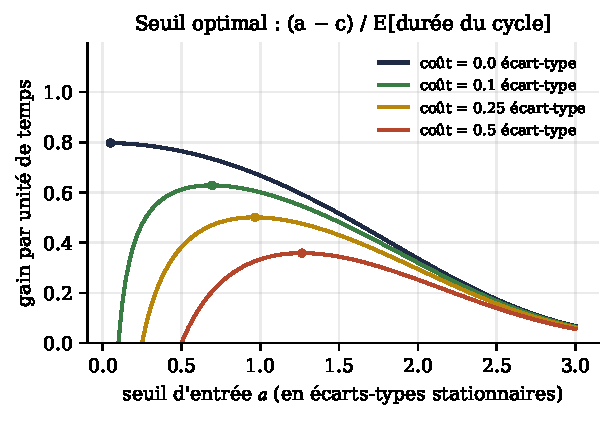
\includegraphics[width=0.62\textwidth]{ch05/seuils_optimaux.pdf}
\caption{Gain par unité de temps en fonction du seuil d'entrée pour quatre niveaux de coût. Le point marque l'optimum.}
\label{c5:fig:opt}
\end{figure}

\begin{pitfall}
Le gain \og offert\fg{} par le dépassement en temps discret est une illusion de \emph{backtest} si, dans la réalité, on exécute par ordres limites au seuil (on n'obtient jamais mieux que le seuil, et l'on n'est exécuté que quand le prix traverse, souvent au pire moment : chapitre~15) ou si l'on exécute au marché le lendemain (on paie le retour partiel). Un \emph{backtest} de \emph{pairs trading} au prix de clôture surestime systématiquement les stratégies à seuils serrés.
\end{pitfall}

\subsection{Seuils et incertitude sur les paramètres}

Le seuil optimal dépend de $\theta$, $\mu$ et $\sigma$. Or E2 a montré que $\theta$ est surestimé et que $\mu$ est mal connu sur un an. Un seuil optimisé sur des paramètres estimés est donc lui-même incertain, et généralement trop serré (car $\theta$ surestimé fait croire que les cycles sont plus courts). En pratique : corriger le biais de $\hat\theta$, élargir légèrement les seuils et vérifier la robustesse sur une plage de paramètres plutôt qu'en un point.

% =====================================================================
\section{Étude de cas : l'écart GLD/GLDM}
% =====================================================================

Sur l'écart GLD/GLDM sans tendance (chapitre~3), $\hat\varphi = 0{,}011$ à l'échelle quotidienne : un OU avec $\theta\Delta = -\ln 0{,}011 \approx 4{,}5$, c'est-à-dire une demi-vie d'environ $0{,}15$ jour, soit une heure de bourse. À l'échelle quotidienne, l'écart (écart-type $4{,}5$ pb) est indiscernable d'un bruit blanc. La modélisation OU n'a d'intérêt que si l'on observe le processus à une fréquence comparable à sa demi-vie : pour cet écart, des données intrajournalières seraient indispensables.

% =====================================================================
\section{Ce que la théorie apporte, et ses limites}
% =====================================================================

\paragraph{Apports.} Un modèle à trois paramètres interprétables ($\theta$, $\mu$, $\sigma$), une correspondance exacte avec l'AR(1) à toute fréquence, des formules de durée de détention et un critère explicite pour choisir les seuils en fonction des coûts.

\paragraph{Limites.} (1) Les chocs browniens sont gaussiens ; les écarts réels ont des queues épaisses et des sauts (annonces de résultats, dividendes). (2) Les paramètres sont supposés constants. (3) Le critère \og gain par unité de temps\fg{} ignore le risque : un seuil qui maximise l'espérance peut avoir une variance déplaisante ; il ignore aussi le capital immobilisé et la marge. (4) La surveillance discrète, l'exécution et les coûts réels changent les résultats, surtout pour les seuils serrés.

% =====================================================================
\section{Fiche à recopier au tableau blanc}
% =====================================================================

\begin{whiteboard}
\begin{itemize}[leftmargin=1.2em]
\item \textbf{Brownien :} $W_t - W_s\sim\N(0,t-s)$, $(\dd W)^2 = \dd t$.
\item \textbf{Itô :} $\dd f = (\partial_tf + b\,\partial_xf + \frac12s^2\partial_{xx}f)\dd t + s\,\partial_xf\,\dd W$.
\item \textbf{OU :} $\dd X = \theta(\mu - X)\dd t + \sigma\dd W$ ; $X_t = \mu + (X_0-\mu)e^{-\theta t} + \sigma\int_0^te^{-\theta(t-u)}\dd W_u$.
\item \textbf{Moments :} moyenne $\mu + (X_0-\mu)e^{-\theta t}$ ; variance $\frac{\sigma^2}{2\theta}(1-e^{-2\theta t})$ ; $\sigma_{eq} = \sigma/\sqrt{2\theta}$ ; $h_{1/2} = \ln2/\theta$.
\item \textbf{OU $\leftrightarrow$ AR(1) :} $\varphi = e^{-\theta\Delta}$, $\sigma_\eta^2 = \frac{\sigma^2}{2\theta}(1-\varphi^2)$ ; $\hat\theta = -\ln\hat\varphi/\Delta$.
\item \textbf{Kolmogorov :} $\frac12s^2u'' + bu' = -1$.
\item \textbf{Retour :} $T_{a\to0} = \frac2{\sigma^2}\int_0^ae^{ky^2}\int_y^\infty e^{-kz^2}\dd z\,\dd y$, $k=\theta/\sigma^2$.
\item \textbf{Seuil optimal :} maximiser $(a-c)/(T_{0\to\pm a}+T_{a\to0})$ ; le seuil monte avec les coûts.
\end{itemize}
\end{whiteboard}

% =====================================================================
\section{Exercices}
% =====================================================================

\begin{exercise}
Appliquez le lemme d'Itô à $f(x) = x^2$ pour un mouvement brownien $X = W$. Déduisez-en $\E[W_t^2] = t$.
\end{exercise}

\begin{exercise}
Un écart quotidien a $\hat\varphi = 0{,}96$ et un écart-type des résidus de 0,5\,\%. Calculez $\theta$ (par an), la demi-vie en jours et l'écart-type stationnaire.
\end{exercise}

\begin{exercise}
Montrez, en dérivant l'intégrale de la proposition~\ref{c5:prop:fpt}, que pour un petit seuil $a$, $T_{a\to0}\approx a\sqrt{\pi/\theta}/\sigma$. Pourquoi ce temps tend-il vers 0 avec $a$ alors que celui d'un mouvement brownien sans dérive serait infini en moyenne ?
\end{exercise}

\begin{exercise}[à coder]
Ajoutez à E4 un stop-loss : on ferme à perte si l'écart atteint $\pm L$ avec $L > a$. Comment le seuil optimal et le gain changent-ils pour $L = 3\sigma_{eq}$ ? Comparez à \citet{leungli2015}.
\end{exercise}

\begin{exercise}[à coder]
Reprenez E2 avec la correction de Kendall appliquée à $\hat\varphi$ avant de calculer $\hat\theta$. Quel est le nouveau biais médian sur un an ?
\end{exercise}

% =====================================================================
\section{Pour aller plus loin}
% =====================================================================

\begin{toread}
\begin{itemize}[leftmargin=1.2em]
\item \citet{uhlenbeck1930} : l'article original, en physique.
\item \citet{bertram2010} : expressions analytiques du gain et de la durée des cycles, et seuils optimaux.
\item \citet{leungli2015} et les premiers chapitres du livre \citet{leungli2016} : entrée et sortie optimales avec coûts et stop-loss.
\item \citet{avellaneda2010}, l'annexe sur l'estimation des paramètres OU à partir d'une régression AR(1), reprise au chapitre~10.
\end{itemize}
\end{toread}

\section{Scripts du chapitre}
\noindent\texttt{code/ch05/ch05\_ornstein\_uhlenbeck.py} : E1 (figure~\ref{c5:fig:paths}), E2, E3, E4 (figure~\ref{c5:fig:opt}), E5.


\part{Les méthodes de pairs trading}
% =====================================================================
\chapter{La méthode des distances}
\label{ch:6}
% =====================================================================

\section{Objectifs et organisation du chapitre}

\paragraph{Objectifs.} La méthode des distances de \citet{gatev2006} est la référence empirique du \emph{pairs trading} : simple, non paramétrique, et testée sur quarante ans de données. À la fin du chapitre, vous saurez : (1) répliquer exactement le protocole de Gatev, Goetzmann et Rouwenhorst (GGR) ; (2) calculer correctement les rendements d'une stratégie de paires (capital engagé, capital employé) ; (3) expliquer pourquoi le critère de sélection par distance est imparfait ; (4) mesurer l'effet des coûts et du nombre de paires ; (5) interpréter les résultats de la littérature qui a suivi.

\paragraph{Code.} \texttt{code/ch06/ch06\_distance\_method.py} et l'univers simulé \texttt{code/common/universe.py}.

% =====================================================================
\section{Le protocole de Gatev, Goetzmann et Rouwenhorst}
% =====================================================================

\subsection{Formation}

Sur une \emph{période de formation} de douze mois, on calcule pour chaque action $i$ un indice de rendement total normalisé à 1 au premier jour, $\tilde P_{i,t} = P_{i,t}/P_{i,0}$ (dividendes réinvestis). Pour chaque paire $(i,j)$, on calcule la somme des écarts quadratiques
\[
\mathrm{SSD}_{ij} = \sum_{t=1}^{T_f}\big(\tilde P_{i,t} - \tilde P_{j,t}\big)^2,
\]
et l'on retient les 20 paires de plus petite SSD : celles dont les trajectoires normalisées se sont le plus suivies. On note aussi l'écart-type $\hat\sigma_{ij}$ de l'écart $\tilde P_i - \tilde P_j$ sur la formation.

\paragraph{Calcul efficace.} Pour $N$ actions il y a $N(N-1)/2$ paires (4\,950 pour 100 actions). En notant $\tilde P$ la matrice $T_f\times N$, $\mathrm{SSD}_{ij} = \|\tilde P_i\|^2 + \|\tilde P_j\|^2 - 2\tilde P_i^\top\tilde P_j$ : toutes les distances s'obtiennent par un seul produit matriciel $\tilde P^\top\tilde P$.

\subsection{Trading}

Pendant les six mois suivants, les prix sont renormalisés à 1 au début de la période. Pour chaque paire retenue :
\begin{itemize}
\item on \textbf{ouvre} une position quand l'écart normalisé dépasse $2\hat\sigma_{ij}$ : achat d'un dollar de l'action relativement bon marché, vente à découvert d'un dollar de l'action relativement chère ;
\item on \textbf{ferme} quand les prix normalisés se recroisent, ou à la fin de la période ;
\item la paire peut rouvrir plusieurs fois.
\end{itemize}
GGR décalent l'exécution d'un jour (signal à la clôture $t$, exécution à la clôture $t+1$) pour neutraliser l'effet du rebond entre prix acheteur et vendeur, et montrent que ce décalage réduit les profits.

\subsection{Mesurer le rendement}

Une position longue d'un dollar et courte d'un dollar ne coûte rien (en théorie) : le \og rendement\fg{} d'une paire n'a de sens que rapporté à un capital conventionnel. GGR proposent deux mesures :
\begin{itemize}
\item \textbf{capital engagé} : somme des gains des 20 paires divisée par 20, que les paires aient tradé ou non. C'est la mesure prudente, celle d'un gestionnaire qui réserve un dollar par paire ;
\item \textbf{capital employé} : somme des gains divisée par le nombre de paires qui ont effectivement ouvert une position.
\end{itemize}
Le gain d'une position ouverte en $t_0$ et fermée en $t_1$ vaut $\big(P^L_{t_1}/P^L_{t_0} - 1\big) - \big(P^C_{t_1}/P^C_{t_0} - 1\big)$, où $L$ est la jambe longue et $C$ la jambe courte.

\begin{intuition}
La SSD cherche deux voitures qui ont roulé côte à côte pendant un an. Pendant les six mois suivants, si l'une prend de l'avance, on parie qu'elles vont se retrouver. Le pari est bon si elles roulent vraiment ensemble (même route, même destination) ; il est mauvais si elles se sont seulement trouvées côte à côte par hasard.
\end{intuition}

% =====================================================================
\section{Ce que dit la littérature}
% =====================================================================

Sur les actions américaines de 1962 à 2002, GGR obtiennent pour les 20 meilleures paires des rendements excédentaires annualisés pouvant atteindre de l'ordre de 11\,\% selon la mesure de capital retenue, avec une faible exposition aux facteurs de risque usuels. \citet{dofaff2010} montrent que ces profits baissent fortement à partir des années 1990, tout en restant positifs dans les périodes de crise (quand la dispersion entre actions augmente). \citet{dofaff2012} ajoutent des coûts de transaction réalistes (commissions, impact, coût d'emprunt des titres) : la stratégie de base devient à peine rentable, et seule une sélection plus fine (même sous-secteur, nombre de croisements élevé pendant la formation) préserve un profit. \citet{rad2016} confirment, avec un protocole identique pour trois méthodes, une baisse de rentabilité dans la période récente.

% =====================================================================
\section{Réplication sur un univers simulé}
% =====================================================================

\subsection{L'univers}

Pour savoir si la méthode trouve les \og bonnes\fg{} paires, il faut connaître la vérité. L'univers simulé contient 100 actions réparties en 5 secteurs ; chaque log-prix est la somme d'un facteur de marché, d'un facteur sectoriel et d'une composante propre. Dans chaque secteur, deux paires sont \emph{jumelles} : leurs deux actions partagent la même composante propre de long terme et ne diffèrent que par un écart AR(1) stationnaire ($\varphi = 0{,}95$, écart-type stationnaire d'environ $1{,}3\,\%$). Il y a donc exactement 10 paires cointégrées parmi 4\,950. Six univers de 1\,764 jours donnent 72 semestres de trading.

\begin{codebox}[ — E1 à E3, protocole GGR simulé]
\textbf{Sélection :} en moyenne, $49{,}9\,\%$ des 20 paires retenues sont de vraies paires, soit la quasi-totalité des 10 existantes ; les 10 autres sont des paires d'actions du même secteur qui se sont suivies par hasard. $17{,}7$ paires sur 20 ouvrent au moins une position. \textbf{Gain par paire et par semestre :} $+2{,}10\,\%$ pour une vraie paire, $-1{,}17\,\%$ pour une fausse. \textbf{Portefeuille de 20 paires, capital engagé} (annualisé) : $0{,}93\,\%$ sans coût ; $0{,}35\,\%$ à 5 pb par jambe ; $-0{,}22\,\%$ à 10 pb ; $-1{,}36\,\%$ à 20 pb. \textbf{Nombre de paires} (coût de 5 pb) : 5 paires, $4{,}1\,\%$ ; 10 paires, $3{,}7\,\%$ ; 20 paires, $0{,}35\,\%$ ; 50 paires, $-1{,}1\,\%$.
\end{codebox}

\begin{figure}[h]
\centering
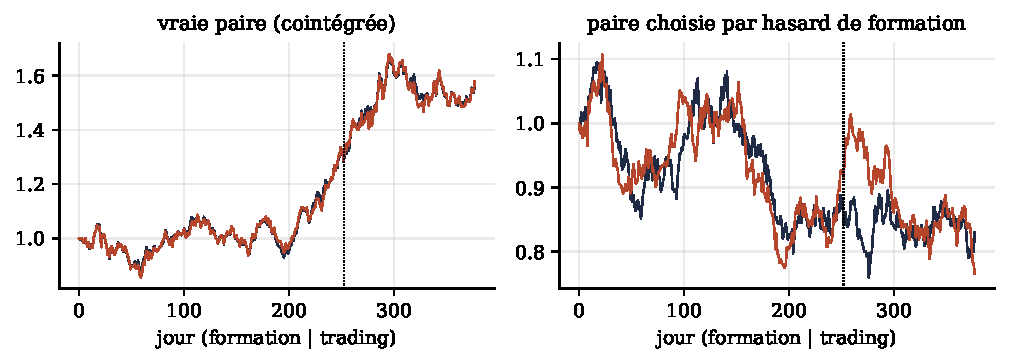
\includegraphics[width=0.95\textwidth]{ch06/ggr_paires.pdf}
\caption{Deux paires du top 20 d'une même formation. À gauche, une vraie paire : les trajectoires restent liées après la formation (ligne pointillée). À droite, une paire retenue parce qu'elle s'est suivie par hasard pendant la formation : elle diverge ensuite.}
\label{c6:fig:pairs}
\end{figure}

\paragraph{Ce que montrent les chiffres.} (1) La SSD classe bien les vraies paires en tête, mais le portefeuille de 20 paires dilue leur profit avec celui de paires fictives qui perdent de l'argent ; c'est pourquoi les 5 ou 10 premières paires font beaucoup mieux que les 20. (2) Les coûts détruisent vite un avantage de quelques dixièmes de pour cent par semestre : à 10 pb par jambe, la stratégie perd de l'argent. (3) Même sans coûts, un tiers des semestres sont perdants.

% =====================================================================
\section{Pourquoi la SSD est un critère imparfait}
% =====================================================================

Développons la SSD. En notant $D_t = \tilde P_{i,t} - \tilde P_{j,t}$ et $\bar D$ sa moyenne sur la formation,
\[
\frac{1}{T_f}\mathrm{SSD}_{ij} = \frac{1}{T_f}\sum_t D_t^2 = \bar D^2 + \widehat{\Var}(D).
\]
Minimiser la SSD revient donc à choisir des paires dont l'écart est petit en moyenne \emph{et peu variable}. Or un \emph{pairs trade} gagne à chaque aller-retour environ deux écarts-types de l'écart (chapitre~1) : une paire à l'écart très peu variable gagne très peu par trade et peine à couvrir ses coûts. La paire idéale a au contraire un écart \emph{ample} et qui revient \emph{vite} à la moyenne : la SSD ne mesure ni l'un ni l'autre \citep{krauss2017survey}.

\begin{pitfall}
La SSD minimale est atteinte par deux actions identiques, par exemple deux lignes de cotation de la même société, ou deux ETF sur le même indice : l'écart est nul, il n'y a rien à gagner. À l'inverse, deux actions qui oscillent fortement l'une autour de l'autre (très bon candidat) ont une SSD plus élevée et peuvent être écartées. Le critère de sélection et le critère de profit ne sont pas les mêmes.
\end{pitfall}

\paragraph{Améliorations proposées.} Restreindre la recherche au même secteur ou sous-secteur \citep{dofaff2012} ; exiger un nombre minimal de croisements de l'écart pendant la formation (indicateur direct de retour à la moyenne) ; combiner distance et test de cointégration \citep{huck2009,rad2016} ; normaliser l'écart par sa volatilité, ce qui conduit au \emph{z-score} du chapitre~1.

% =====================================================================
\section{Études de cas réelles}
% =====================================================================

On applique la règle GGR à nos deux paires réelles : formation sur les 252 premières séances, trading sur les 248 suivantes.

\begin{codebox}[ — E4, règle GGR sur données réelles]
\textbf{KO/PEP :} l'écart normalisé a déjà un écart-type de $9{,}6\,\%$ pendant la formation (les deux titres ont divergé). Une seule position est ouverte pendant la période de trading et ne se referme jamais : perte de $24{,}1\,\%$ avant coûts. \textbf{GLD/GLDM :} écart-type de formation de $0{,}135\,\%$ ; une position, gain brut nul ($-0{,}01\,\%$), $-0{,}21\,\%$ après coûts de 5 pb par jambe.
\end{codebox}

\paragraph{Lecture.} KO/PEP illustre le risque central de la méthode : une paire qui ne revient pas, gardée jusqu'à la fin de la période faute de stop-loss. GLD/GLDM illustre l'autre extrême : un écart si petit qu'aucun trade ne couvre ses coûts. Ces deux cas sont les deux faces du problème décrit à la section précédente.

% =====================================================================
\section{Ce que la théorie apporte, et ses limites}
% =====================================================================

\paragraph{Apports.} Un protocole simple et reproductible, une référence pour comparer toutes les autres méthodes, une définition claire du rendement d'une stratégie autofinancée, et la preuve historique qu'un avantage a existé.

\paragraph{Limites.} Pas de modèle de l'écart, donc pas de demi-vie ni de seuil optimal ; ratio de couverture implicite de 1 dollar contre 1 dollar, sans justification statistique ; sélection biaisée vers les écarts peu volatils ; profits historiques en déclin et très sensibles aux coûts, au coût d'emprunt et au décalage d'exécution.

% =====================================================================
\section{Fiche à recopier au tableau blanc}
% =====================================================================

\begin{whiteboard}
\begin{itemize}[leftmargin=1.2em]
\item \textbf{Formation 12 mois :} $\tilde P_{i,t} = P_{i,t}/P_{i,0}$, $\mathrm{SSD}_{ij} = \sum_t(\tilde P_{i,t}-\tilde P_{j,t})^2$, top 20 paires.
\item \textbf{Calcul matriciel :} $\mathrm{SSD} = \mathrm{diag}(G)\mathbf 1^\top + \mathbf 1\mathrm{diag}(G)^\top - 2G$, $G = \tilde P^\top\tilde P$.
\item \textbf{Trading 6 mois :} ouvrir à $|D_t| > 2\hat\sigma$ (1\,\$ long / 1\,\$ court), fermer au croisement.
\item \textbf{Gain d'un trade :} $(P^L_{t_1}/P^L_{t_0}-1) - (P^C_{t_1}/P^C_{t_0}-1)$.
\item \textbf{Capital engagé :} somme des gains / 20 ; \textbf{employé :} / nombre de paires ouvertes.
\item \textbf{Biais de la SSD :} $\mathrm{SSD}/T = \bar D^2 + \widehat\Var(D)$ : favorise les écarts peu volatils.
\end{itemize}
\end{whiteboard}

% =====================================================================
\section{Exercices}
% =====================================================================

\begin{exercise}
Démontrez l'identité $\frac1T\sum_tD_t^2 = \bar D^2 + \widehat\Var(D)$ (avec la variance empirique divisée par $T$).
\end{exercise}

\begin{exercise}
Une paire a un écart de formation d'écart-type $1\,\%$. Les coûts sont de 5 pb par jambe et par transaction. Quel gain minimal (en écarts-types) doit capturer un aller-retour pour être rentable ?
\end{exercise}

\begin{exercise}[à coder]
Ajoutez à \texttt{trade\_pair} un décalage d'exécution d'un jour (signal en $t$, exécution en $t+1$) et un stop-loss à $4\hat\sigma$. Mesurez l'effet de chacun sur les vraies et les fausses paires.
\end{exercise}

\begin{exercise}[à coder]
Remplacez le critère SSD par : SSD minimale \emph{parmi les paires du même secteur ayant au moins 8 croisements pendant la formation}. La part de vraies paires dans le top 20 augmente-t-elle ? Et le rendement ?
\end{exercise}

% =====================================================================
\section{Pour aller plus loin}
% =====================================================================

\begin{toread}
\begin{itemize}[leftmargin=1.2em]
\item \citet{gatev2006} : la section sur la méthodologie (formation, trading, calcul des rendements) et les tests de robustesse au décalage d'exécution.
\item \citet{dofaff2010,dofaff2012} : l'évolution des profits dans le temps et l'effet des coûts.
\item \citet{krauss2017survey}, la partie consacrée à l'approche par distance : synthèse des variantes et de leurs critiques.
\end{itemize}
\end{toread}

\section{Scripts du chapitre}
\noindent\texttt{code/ch06/ch06\_distance\_method.py} : E1–E3 (protocole GGR simulé, figure~\ref{c6:fig:pairs}), E4 (données réelles). Univers : \texttt{code/common/universe.py}.

% =====================================================================
\chapter{Cointégration appliquée : sélectionner les paires sans se mentir}
\label{ch:7}
% =====================================================================

\section{Objectifs et organisation du chapitre}

\paragraph{Objectifs.} Le chapitre~4 a donné les tests de cointégration pour \emph{une} paire. En pratique, on teste des centaines ou des milliers de paires candidates, et c'est là que la plupart des stratégies échouent : on retient surtout des faux positifs. À la fin de ce chapitre, vous saurez : (1) quantifier le nombre de faux positifs d'une recherche de paires ; (2) appliquer les corrections de Bonferroni et de Benjamini-Hochberg ; (3) construire un pipeline de sélection qui combine a priori économique, test statistique et filtres de dynamique \citep{vidyamurthy2004,huck2009,krauss2017survey} ; (4) mesurer la performance hors échantillon des paires retenues ; (5) choisir entre ratio de couverture statique et glissant.

\paragraph{Code.} \texttt{code/ch07/ch07\_cointegration\_selection.py}, univers \texttt{code/common/universe.py}.

% =====================================================================
\section{Le problème des tests multiples}
% =====================================================================

\subsection{Combien de faux positifs ?}

Avec $N$ actions, il y a $m = N(N-1)/2$ paires. Si l'on teste chacune au seuil $\alpha$ et qu'aucune n'est cointégrée, le nombre de rejets suit à peu près une loi binomiale de paramètres $(m,\alpha)$ : on attend $m\alpha$ faux positifs. Pour $N = 100$, $m = 4\,950$ et $\alpha = 5\,\%$, cela fait environ 250 \og paires cointégrées\fg{} purement fortuites.

\begin{intuition}
Lancez 4\,950 pièces de monnaie dix fois chacune : quelques-unes tomberont huit ou neuf fois sur pile. Ce ne sont pas des pièces truquées, ce sont les plus chanceuses. Si vous les \og sélectionnez\fg{} pour les relancer, elles retomberont à la moyenne. Une paire qui a passé le test par chance se comporte de même hors échantillon.
\end{intuition}

\subsection{Deux façons de contrôler l'erreur}

\begin{definition}
Parmi $m$ tests, on note $V$ le nombre de faux positifs (hypothèses nulles vraies rejetées) et $R$ le nombre total de rejets.
\begin{itemize}
\item Le \emph{taux d'erreur par famille} (FWER) est $\Prob(V\ge1)$ : la probabilité de commettre au moins une fausse découverte.
\item Le \emph{taux de fausses découvertes} (FDR) est $\E[V/\max(R,1)]$ : la proportion attendue de fausses découvertes parmi les découvertes.
\end{itemize}
\end{definition}

\begin{proposition}[Bonferroni]
Si l'on rejette chaque hypothèse dont la $p$-valeur est inférieure à $\alpha/m$, alors $\mathrm{FWER}\le\alpha$, quelle que soit la dépendance entre les tests.
\end{proposition}
\begin{proof}
Soit $I_0$ l'ensemble des hypothèses nulles vraies, de taille $m_0\le m$. Sous une hypothèse nulle vraie, $\Prob(p_i\le\alpha/m) \le \alpha/m$ (propriété d'une $p$-valeur valide). Par l'inégalité de la réunion, $\Prob(V\ge1) = \Prob\big(\bigcup_{i\in I_0}\{p_i\le\alpha/m\}\big) \le \sum_{i\in I_0}\alpha/m = m_0\alpha/m \le \alpha$.
\end{proof}

Bonferroni est très conservateur : avec 4\,950 tests, il exige $p < 10^{-5}$. La procédure de Benjamini-Hochberg contrôle plutôt la proportion de fausses découvertes, ce qui convient mieux à une recherche de paires (on accepte quelques erreurs si la plupart des paires retenues sont bonnes).

\paragraph{Procédure de Benjamini-Hochberg (BH).} On ordonne les $p$-valeurs $p_{(1)}\le p_{(2)}\le\dots\le p_{(m)}$, on cherche le plus grand $k$ tel que $p_{(k)}\le kq/m$, et l'on rejette les $k$ hypothèses correspondantes. Sous indépendance des tests (ou une forme de dépendance positive), cette procédure garantit $\mathrm{FDR}\le q$.

\begin{pitfall}
Les tests de cointégration d'un même univers sont fortement dépendants : deux paires qui partagent une action, ou deux actions du même secteur, ont des statistiques corrélées. Les garanties théoriques de BH ne sont alors qu'approximatives. Surtout, \emph{toute} la recherche compte : si vous avez essayé trois fenêtres, deux sens de régression et deux spécifications de tendance, vous avez fait douze fois plus de tests que vous ne le pensez.
\end{pitfall}

% =====================================================================
\section{Un pipeline de sélection}
% =====================================================================

La littérature et la pratique convergent vers une sélection en plusieurs filtres, du moins coûteux au plus exigeant :
\begin{enumerate}
\item \textbf{A priori économique.} Restreindre les candidats aux actifs qui ont une raison de rester liés : même secteur ou sous-secteur, même sous-jacent, relation contractuelle (ETF et panier, deux catégories d'actions d'une même société). Cela réduit $m$ d'un facteur 5 à 50 et élimine les relations purement fortuites.
\item \textbf{Test de cointégration} (Engle-Granger dans les deux sens, ou Johansen), avec correction des tests multiples.
\item \textbf{Filtres de dynamique.} Demi-vie dans une plage exploitable (assez courte pour trader, assez longue pour couvrir les coûts) ; amplitude de l'écart suffisante par rapport aux coûts (chapitre~5) ; nombre de croisements de la moyenne.
\item \textbf{Stabilité.} La relation est-elle détectée sur plusieurs sous-périodes ? Le ratio de couverture est-il stable ?
\item \textbf{Contraintes pratiques.} Liquidité des deux jambes, disponibilité et coût de l'emprunt de titres pour la vente à découvert, frais.
\end{enumerate}

% =====================================================================
\section{Expérience : 4\,950 paires, 10 vraies}
% =====================================================================

On reprend l'univers simulé du chapitre~6 (100 actions, 5 secteurs, 10 paires réellement cointégrées) avec une formation de 500 jours et un trading hors échantillon de 250 jours (règle \emph{z-score} du chapitre~1, entrée à $\pm2$, sortie à 0, coûts de 5 pb par jambe). On distingue trois sortes de paires : les \emph{vraies} paires ; les paires \emph{partiellement liées}, dont une jambe appartient à une vraie paire (leur écart contient la moitié de l'écart stationnaire de la vraie paire, comme dans la cointégration partielle du chapitre~4) ; les paires \emph{sans lien}, dont l'écart est une martingale. Deux scénarios : vraies paires de demi-vie 4,3 jours ($\varphi = 0{,}85$) ou 13,5 jours ($\varphi = 0{,}95$). Douze univers par scénario.

\begin{table}[h]
\centering\small
\caption{Paires retenues par univers (moyenne sur 12 univers), selon la règle de sélection.}
\label{c7:tab:sel}
\begin{tabular}{lccccc}
\toprule
 & \multicolumn{2}{c}{Demi-vie 4,3 j} & & \multicolumn{2}{c}{Demi-vie 13,5 j}\\
\cmidrule{2-3}\cmidrule{5-6}
Règle & vraies & fausses & & vraies & fausses \\
\midrule
$p<5\,\%$ (4\,950 tests) & 10,0 & 265,2 & & 8,4 & 264,3 \\
Bonferroni & 9,0 & 0,0 & & 0,1 & 0,0 \\
Benjamini-Hochberg, $q = 5\,\%$ & 10,0 & 0,9 & & 0,1 & 0,0 \\
Même secteur (950 tests) $+$ BH & 10,0 & 0,7 & & 0,3 & 0,1 \\
\bottomrule
\end{tabular}
\end{table}

\begin{codebox}[ — E1 et E2, sélection et performance hors échantillon]
\textbf{Sélection} (tableau~\ref{c7:tab:sel}) : sans correction, 96\,\% des paires retenues sont fausses. Avec BH, presque toutes sont vraies \emph{si} le retour à la moyenne est rapide ; si la demi-vie est de 13,5 jours, 500 jours de formation ne suffisent plus à franchir le seuil corrigé et l'on ne retient presque rien. \textbf{Rendement hors échantillon par paire} (250 jours, en \% du notionnel brut, moyenne des moyennes par univers $\pm$ erreur-type entre univers, scénario 4,3 j) : vraies paires $3{,}71 \pm 0{,}14$ ; paires partiellement liées $3{,}49 \pm 1{,}93$ ; paires sans lien $1{,}69 \pm 1{,}61$. Les moyennes par univers des paires sans lien vont de $-4{,}5\,\%$ à $+13{,}1\,\%$, celles des paires partiellement liées de $-7{,}6\,\%$ à $+17{,}2\,\%$, celles des vraies paires de $3{,}0\,\%$ à $4{,}6\,\%$.
\end{codebox}

\begin{figure}[h]
\centering
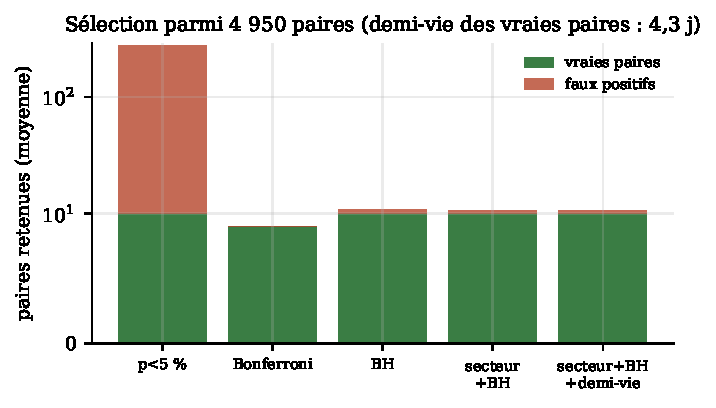
\includegraphics[width=0.7\textwidth]{ch07/selection_faux_positifs.pdf}
\caption{Paires retenues par univers selon la règle (échelle logarithmique au-delà de 10). Sans correction, les vraies paires (vert) sont noyées sous les faux positifs (rouge).}
\label{c7:fig:sel}
\end{figure}

\paragraph{Trois leçons.}
\begin{enumerate}
\item \textbf{Les faux positifs ne perdent pas forcément d'argent en moyenne, ils ajoutent du risque.} Une paire sans lien a une espérance de gain nulle (l'écart est une martingale), mais une variance énorme : la moyenne d'un univers à l'autre oscille entre $-4{,}5$ et $+13{,}1\,\%$. Une petite moyenne positive sur un échantillon n'est pas une preuve. Remarquez aussi que l'erreur-type \og naïve\fg, qui traite les paires comme indépendantes, vaut $0{,}36\,\%$ alors que l'erreur-type correcte entre univers vaut $1{,}61\,\%$ : des paires qui partagent des actions ne sont pas des observations indépendantes.
\item \textbf{Les relations partielles existent et rapportent, mais de façon instable.} Les paires partiellement liées gagnent en moyenne autant que les vraies, avec une dispersion entre univers environ quatorze fois plus grande.
\item \textbf{La correction a un prix : la puissance.} Quand la demi-vie est longue, la correction pour tests multiples supprime aussi les vraies paires. Il faut alors plus d'historique, des données plus fréquentes si la dynamique le permet, ou un a priori économique plus serré qui réduit le nombre de tests.
\end{enumerate}

\begin{codebox}[ — E3, persistance des paires retenues]
Parmi les 131 paires retenues par BH (scénario 4,3 j, 12 univers), 122 sont de nouveau cointégrées à 5\,\% sur la fenêtre suivante (décalée de 250 jours), dont 120 vraies. La stabilité dans le temps est un excellent filtre complémentaire : une relation réelle se retrouve d'une fenêtre à l'autre.
\end{codebox}

% =====================================================================
\section{Ratio de couverture : statique ou glissant ?}
% =====================================================================

Une fois la paire retenue, faut-il garder le $\hat\beta$ estimé sur la formation ou le réestimer en continu sur une fenêtre glissante ? Une fenêtre glissante s'adapte aux changements, mais chaque réestimation sur peu de données ajoute du bruit, et ce bruit se transforme en P\&L parasite : l'écart \og bouge\fg{} parce que $\beta$ bouge, pas parce que les prix ont bougé.

\begin{codebox}[ — E4, erreur sur le ratio quand le vrai ratio est constant]
Erreur absolue moyenne sur $\beta$ (vrai $\beta = 1$, 30 vraies paires) : statique sur 500 jours $0{,}026$ ; glissant sur 250 jours $0{,}033$ ; glissant sur 60 jours $0{,}073$.
\end{codebox}

Quand la relation est stable, la fenêtre glissante courte est presque trois fois moins précise. Elle ne se justifie que si le ratio change réellement ; et dans ce cas, le filtre de Kalman du chapitre~8 fait le même travail de façon optimale, en dosant automatiquement la réactivité.

% =====================================================================
\section{Dimensionner les positions}
% =====================================================================

Pour que chaque paire contribue au risque de façon comparable, on dimensionne la position par la volatilité de l'écart plutôt qu'en montant fixe : si l'écart (en log) a un écart-type quotidien $\sigma_S$, une position de notionnel $K$ sur la jambe $Y$ a un risque quotidien d'environ $K\sigma_S$. Viser un risque cible $R$ par paire donne $K = R/\sigma_S$. On limite ensuite le notionnel total, l'exposition par secteur et l'exposition au facteur de marché résiduel (si $\hat\beta$ diffère des expositions réelles au marché, la paire n'est pas neutre). Le chapitre~17 traite le dimensionnement global.

% =====================================================================
\section{Ce que la théorie apporte, et ses limites}
% =====================================================================

\paragraph{Apports.} Un cadre pour savoir combien de découvertes sont crédibles, une procédure qui garde la proportion de fausses paires sous contrôle, et un pipeline qui combine information économique et statistique.

\paragraph{Limites.} Les corrections supposent que l'on compte honnêtement tous les tests ; la dépendance entre tests affaiblit les garanties ; la puissance chute quand les demi-vies sont longues ; et la cointégration passée ne garantit rien sur l'avenir : il faut surveiller les paires en continu et les retirer quand la relation se dégrade (chapitre~17).

% =====================================================================
\section{Fiche à recopier au tableau blanc}
% =====================================================================

\begin{whiteboard}
\begin{itemize}[leftmargin=1.2em]
\item \textbf{Faux positifs attendus :} $m\alpha$, avec $m = N(N-1)/2$.
\item \textbf{FWER} $=\Prob(V\ge1)$ ; \textbf{FDR} $=\E[V/\max(R,1)]$.
\item \textbf{Bonferroni :} rejeter si $p < \alpha/m$ ; preuve par l'inégalité de la réunion.
\item \textbf{BH :} plus grand $k$ tel que $p_{(k)}\le kq/m$ ; rejeter les $k$ plus petites.
\item \textbf{Pipeline :} a priori économique $\to$ test corrigé $\to$ demi-vie et amplitude $\to$ stabilité $\to$ contraintes pratiques.
\item \textbf{Erreur-type honnête :} regrouper par univers ou période, jamais par paire si les paires partagent des actifs.
\item \textbf{Taille :} notionnel $K = R/\sigma_S$.
\end{itemize}
\end{whiteboard}

% =====================================================================
\section{Exercices}
% =====================================================================

\begin{exercise}
Pour 30 actions d'un même secteur, combien de paires ? Quel seuil de Bonferroni à 5\,\% ? Combien de faux positifs attendus sans correction ?
\end{exercise}

\begin{exercise}
Appliquez BH à la main avec $q = 10\,\%$ aux $p$-valeurs $0{,}001$ ; $0{,}008$ ; $0{,}039$ ; $0{,}041$ ; $0{,}042$ ; $0{,}06$ ; $0{,}074$ ; $0{,}205$ ; $0{,}212$ ; $0{,}216$. Combien de rejets ? Combien avec Bonferroni ?
\end{exercise}

\begin{exercise}
Pourquoi les paires partiellement liées de l'expérience gagnent-elles de l'argent alors qu'aucune n'est cointégrée ? Reliez votre réponse à la proposition~\ref{c4:prop:r2mr}.
\end{exercise}

\begin{exercise}[à coder]
Ajoutez au pipeline un filtre \og demi-vie entre 2 et 20 jours\fg{} et un filtre de stabilité (cointégration sur chacune des deux moitiés de la formation). Mesurez l'effet sur la part de vraies paires dans le scénario de demi-vie 13,5 jours sans correction BH.
\end{exercise}

\begin{exercise}[données réelles]
Construisez un univers d'une vingtaine d'actions d'un même secteur (téléchargées via Interactive Brokers) et appliquez le pipeline complet. Combien de paires survivent à BH ? Combien sont encore cointégrées six mois plus tard ?
\end{exercise}

% =====================================================================
\section{Pour aller plus loin}
% =====================================================================

\begin{toread}
\begin{itemize}[leftmargin=1.2em]
\item \citet{vidyamurthy2004} : les chapitres consacrés à la sélection des paires et au test de la tendance commune.
\item \citet{huck2009} : une méthode de classement des paires par prévision et surclassement.
\item \citet{rad2016} : protocole de comparaison des méthodes sur longue période.
\item \citet{harvey2016} : les tests multiples en finance empirique, la référence pour comprendre pourquoi les seuils usuels sont trop faibles.
\end{itemize}
\end{toread}

\section{Scripts du chapitre}
\noindent\texttt{code/ch07/ch07\_cointegration\_selection.py} : E1–E2 (tableau~\ref{c7:tab:sel}, figure~\ref{c7:fig:sel}), E3 (persistance), E4 (ratio statique contre glissant).

% =====================================================================
\chapter{Modèles espace-état et filtre de Kalman}
\label{ch:8}
% =====================================================================

\section{Objectifs et organisation du chapitre}

\paragraph{Objectifs.} Les chapitres précédents ont supposé un ratio de couverture constant. Dans la réalité, la relation entre deux actifs dérive. Le filtre de Kalman estime en temps réel des quantités cachées qui évoluent (un ratio de couverture, la composante stationnaire d'un écart) à partir d'observations bruitées. À la fin du chapitre, vous saurez : (1) écrire un modèle espace-état ; (2) dériver les équations du filtre de Kalman à partir du conditionnement gaussien ; (3) l'appliquer à une régression à coefficients variables et à l'estimation de la cointégration partielle ; (4) régler ses paramètres sans tomber dans le piège de la vraisemblance ; (5) en tirer un signal de trading.

\paragraph{Code.} \texttt{code/ch08/ch08\_kalman.py}, expériences E1 à E5.

% =====================================================================
\section{Le modèle espace-état}
% =====================================================================

\begin{definition}
Un modèle espace-état linéaire gaussien comprend :
\begin{align*}
\text{équation d'état :}\quad & \xi_t = F\,\xi_{t-1} + w_t, & w_t\sim\N(0,Q),\\
\text{équation d'observation :}\quad & y_t = H_t\,\xi_t + v_t, & v_t\sim\N(0,R),
\end{align*}
où $\xi_t$ est l'état caché (non observé), $y_t$ l'observation, $F$ la matrice de transition, $H_t$ la matrice d'observation (qui peut dépendre du temps), et $w_t$, $v_t$ des bruits indépendants.
\end{definition}

\begin{intuition}
Vous suivez un bateau dans le brouillard. Vous savez à peu près comment il se déplace (équation d'état, avec une part d'imprévu), et de temps en temps un radar vous donne une position imprécise (équation d'observation). Le filtre de Kalman combine ces deux sources pour donner, à chaque instant, la meilleure estimation de la position et son incertitude. Il fait confiance au radar quand la prévision est incertaine, et à la prévision quand le radar est imprécis.
\end{intuition}

\paragraph{Exemples en arbitrage statistique.}
\begin{itemize}
\item \textbf{Ratio de couverture variable :} $\xi_t = (\alpha_t,\beta_t)^\top$ suit une marche aléatoire ($F = I$), et l'on observe $y_t = \alpha_t + \beta_tx_t + v_t$, donc $H_t = (1, x_t)$.
\item \textbf{Écart observé avec bruit} \citep{elliott2005} : l'état $\xi_t$ est un écart qui revient à la moyenne ($\xi_t = a + b\,\xi_{t-1} + w_t$, $|b|<1$) et l'on observe $y_t = \xi_t + v_t$, où $v_t$ représente le bruit de microstructure.
\item \textbf{Cointégration partielle} \citep{clegg2018} : $\xi_t = (M_t, R_t)^\top$, $F = \mathrm{diag}(\rho,1)$, et l'écart observé est $S_t = M_t + R_t$, donc $H = (1,1)$.
\end{itemize}

% =====================================================================
\section{Les équations du filtre}
% =====================================================================

\subsection{Un résultat de conditionnement gaussien}

\begin{lemma}\label{c8:lem:cond}
Si $(X, Y)$ est un vecteur gaussien de moyenne $(\mu_X,\mu_Y)$ et de covariances $\Sigma_{XX}$, $\Sigma_{XY}$, $\Sigma_{YY}$, alors la loi de $X$ sachant $Y = y$ est gaussienne de moyenne $\mu_X + \Sigma_{XY}\Sigma_{YY}^{-1}(y-\mu_Y)$ et de covariance $\Sigma_{XX} - \Sigma_{XY}\Sigma_{YY}^{-1}\Sigma_{YX}$.
\end{lemma}
\begin{proof}
Posons $Z = X - \Sigma_{XY}\Sigma_{YY}^{-1}Y$. Alors $\Cov(Z, Y) = \Sigma_{XY} - \Sigma_{XY}\Sigma_{YY}^{-1}\Sigma_{YY} = 0$. Pour un vecteur gaussien, covariance nulle signifie indépendance : $Z$ est indépendant de $Y$. Donc, sachant $Y = y$, $X = Z + \Sigma_{XY}\Sigma_{YY}^{-1}y$ a pour moyenne $\E[Z] + \Sigma_{XY}\Sigma_{YY}^{-1}y = \mu_X + \Sigma_{XY}\Sigma_{YY}^{-1}(y - \mu_Y)$ et pour covariance $\Var(Z) = \Sigma_{XX} - \Sigma_{XY}\Sigma_{YY}^{-1}\Sigma_{YX}$ (calcul direct avec la proposition~\ref{c1:prop:varspread} généralisée aux matrices).
\end{proof}

\subsection{Prédiction et mise à jour}

Supposons connue la loi de l'état sachant les observations jusqu'à $t-1$ : $\N(m_{t-1}, P_{t-1})$.

\begin{proposition}[Filtre de Kalman]\label{c8:prop:kalman}
\textbf{Prédiction :} $m_{t|t-1} = F m_{t-1}$, \quad $P_{t|t-1} = F P_{t-1}F^\top + Q$.

\textbf{Innovation :} $e_t = y_t - H_tm_{t|t-1}$, de variance $F_t = H_tP_{t|t-1}H_t^\top + R$.

\textbf{Mise à jour :} $K_t = P_{t|t-1}H_t^\top F_t^{-1}$, \quad $m_t = m_{t|t-1} + K_te_t$, \quad $P_t = P_{t|t-1} - K_tH_tP_{t|t-1}$.
\end{proposition}
\begin{proof}
La prédiction découle de l'équation d'état : $\E[F\xi_{t-1} + w_t] = Fm_{t-1}$ et $\Var(F\xi_{t-1} + w_t) = FP_{t-1}F^\top + Q$, car $w_t$ est indépendant du passé. Sachant le passé, le couple $(\xi_t, y_t)$ est gaussien, avec $\E[y_t] = H_tm_{t|t-1}$, $\Var(y_t) = H_tP_{t|t-1}H_t^\top + R = F_t$ et $\Cov(\xi_t, y_t) = P_{t|t-1}H_t^\top$. Le lemme~\ref{c8:lem:cond} avec $X = \xi_t$, $Y = y_t$ donne exactement la mise à jour.
\end{proof}

\paragraph{Lecture dans le cas scalaire.} Avec un état et une observation de dimension 1 et $H = 1$, le gain vaut $K = P/(P+R)$. Si la prévision est très incertaine ($P\gg R$), $K\approx1$ et l'on suit l'observation ; si l'observation est très bruitée ($R\gg P$), $K\approx0$ et l'on garde la prévision. La nouvelle estimation est une moyenne pondérée de la prévision et de l'observation, et sa variance $P(1-K) = PR/(P+R)$ est plus petite que chacune des deux.

\subsection{Vraisemblance}

Les innovations $e_t$ sont indépendantes et de loi $\N(0, F_t)$ sous le modèle. La log-vraisemblance s'écrit donc simplement (décomposition par erreurs de prévision) :
\[
\ell = -\frac12\sum_t\Big(\ln(2\pi F_t) + \frac{e_t^2}{F_t}\Big).
\]
On estime les paramètres inconnus ($Q$, $R$, $\rho$\dots) en maximisant $\ell$, comme au chapitre~2.

% =====================================================================
\section{Ratio de couverture variable}
% =====================================================================

\subsection{Le modèle}

On pose $\xi_t = (\alpha_t, \beta_t)^\top$, $F = I$, $Q = \frac{\delta}{1-\delta}I$ et $H_t = (1, x_t)$, suivant la paramétrisation popularisée par \citet{chan2013} : $\delta$ règle la vitesse à laquelle les coefficients peuvent changer. Avec $\delta\to0$, les coefficients sont constants et le filtre converge vers les MCO récursifs ; avec $\delta$ grand, ils suivent chaque mouvement.

\begin{codebox}[ — E1 et E2, suivi d'un ratio qui dérive]
\textbf{Protocole :} prix simulés, $y_t = 5 + \beta_tx_t + s_t$ avec $\beta_t$ marche aléatoire (pas d'écart-type $0{,}003$) et $s_t$ AR(1) ($\varphi = 0{,}9$) ; 1\,500 jours. \textbf{Erreur quadratique moyenne sur $\beta_t$} (après 250 jours) : Kalman $0{,}017$ avec $\delta = 10^{-7}$ ; $0{,}031$ avec $10^{-6}$ ; $0{,}061$ avec $10^{-5}$ ; $0{,}091$ avec $10^{-4}$. MCO glissants : $0{,}113$ (60 jours), $0{,}039$ (250 jours) ; MCO statique sur la formation : $0{,}048$. \textbf{Log-vraisemblance} : maximale pour $\delta = 10^{-5}$ ($-1\,370$), contre $-1\,928$ pour $\delta = 10^{-7}$.
\end{codebox}

\begin{figure}[h]
\centering
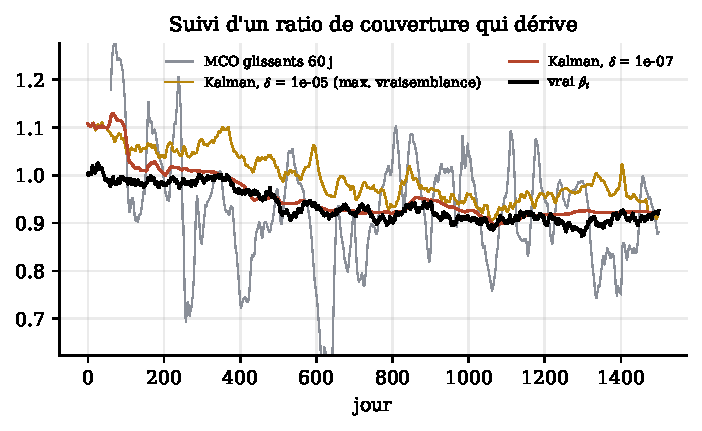
\includegraphics[width=0.75\textwidth]{ch08/kalman_beta.pdf}
\caption{Vrai ratio de couverture (noir), estimations par MCO glissants sur 60 jours, et par filtre de Kalman avec deux réglages. Le réglage qui maximise la vraisemblance (or) suit trop nerveusement ; le réglage lent (rouge) suit la vraie dérive.}
\label{c8:fig:beta}
\end{figure}

\subsection{Le piège de la vraisemblance}

Le réglage qui maximise la vraisemblance n'est pas celui qui suit le mieux $\beta_t$. La raison est importante : dans notre modèle, l'écart $s_t$ est autocorrélé, alors que le filtre suppose un bruit d'observation $v_t$ indépendant. Pour mieux prédire $y_t$, le filtre a intérêt à faire bouger $\alpha_t$ et $\beta_t$ pour absorber la partie prévisible de l'écart. Il gagne en vraisemblance\dots{} en \og mangeant\fg{} l'écart que l'on veut justement trader.

\begin{pitfall}
Un filtre de Kalman trop réactif fait disparaître le signal de retour à la moyenne dans l'état. Le critère de réglage doit correspondre à l'usage : pour un ratio de couverture, choisir $\delta$ petit (ou estimer $\delta$ sur un modèle qui inclut explicitement l'écart comme état AR(1), à la manière d'\citet{elliott2005}) et vérifier hors échantillon le P\&L de la stratégie, pas seulement la vraisemblance.
\end{pitfall}

\subsection{Un signal de trading}

L'innovation $e_t$ est l'écart entre le prix observé de $y$ et sa valeur prédite par la relation estimée : c'est un \emph{spread} à ratio variable, et $\sqrt{F_t}$ son écart-type prédit. Une règle simple : vendre l'écart quand $e_t > \sqrt{F_t}$, l'acheter quand $e_t < -\sqrt{F_t}$, fermer quand $e_t$ change de signe ; le P\&L utilise le ratio de la veille, pour ne pas anticiper.

\begin{codebox}[ — E3, Kalman contre ratio statique]
\textbf{Protocole :} 100 paires simulées avec $\beta_t$ qui dérive, formation de 250 jours, trading de 750 jours, coûts de 5 pb par jambe. \textbf{Résultats} (rendement annuel sur le notionnel brut) : Kalman ($\delta = 10^{-6}$) $6{,}5\,\%$ en moyenne (écart-type $4{,}2\,\%$, 99\,\% de paires gagnantes) ; ratio statique et \emph{z-score} à 2 : $1{,}7\,\%$ (écart-type $2{,}4\,\%$, 72\,\% de paires gagnantes).
\end{codebox}

Quand le ratio dérive réellement, le filtre maintient un écart stationnaire là où le ratio statique laisse l'écart dériver. Quand le ratio est stable (chapitre~7, E4), un filtre lent se comporte comme les MCO et ne coûte presque rien : c'est une assurance peu chère.

% =====================================================================
\section{Estimer la cointégration partielle}
% =====================================================================

Avec l'état $(M_t, R_t)$, $F = \mathrm{diag}(\rho,1)$, $Q = \mathrm{diag}(\sigma_M^2,\sigma_R^2)$, $H = (1,1)$ et un bruit d'observation négligeable, le filtre décompose l'écart observé en une partie qui revient à la moyenne et une partie qui dérive. On estime $(\rho,\sigma_M,\sigma_R)$ par maximum de vraisemblance.

\begin{codebox}[ — E5, cointégration partielle]
\textbf{Protocole :} vrais paramètres $\rho = 0{,}8$, $\sigma_M = 1$, $\sigma_R = 0{,}4$ ($R^2_{MR} = 0{,}874$), 25 écarts de 1\,000 points. \textbf{Résultats} (médianes) : $\hat\rho = 0{,}801$, $\hat\sigma_M = 1{,}005$, $\hat\sigma_R = 0{,}379$, $\hat R^2_{MR} = 0{,}880$ ; intervalle 5–95\,\% de $\hat\rho$ : $[0{,}73\,;\,0{,}84]$. Rappel : sur ce type d'écart, le test ADF du chapitre~4 échouait souvent à détecter quoi que ce soit.
\end{codebox}

En trading, on utilise l'estimation filtrée $\hat M_t$ (et non l'écart brut) pour le signal : on parie sur le retour de la composante stationnaire, pas sur celui de la marche aléatoire.

% =====================================================================
\section{Études de cas réelles}
% =====================================================================

\begin{codebox}[ — E4, ratio de Kalman sur données réelles ($\log$-prix, $\delta = 10^{-5}$)]
\textbf{KO sur PEP :} $\hat\beta_t$ passe de $0{,}76$ (après 30 séances) à $0{,}52$ au milieu de l'échantillon et finit à $0{,}58$. \textbf{GLD sur GLDM :} $\hat\beta_t$ part de $1{,}20$ et converge vers $1{,}02$.
\end{codebox}

\begin{figure}[h]
\centering
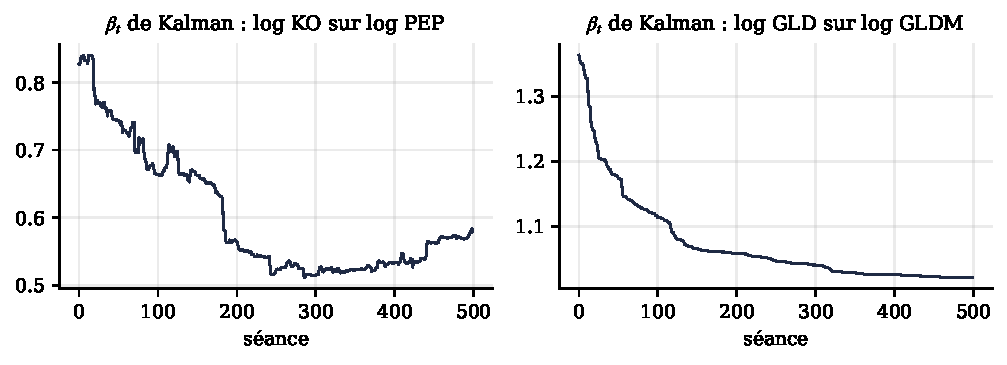
\includegraphics[width=0.95\textwidth]{ch08/kalman_reel.pdf}
\caption{Ratio de couverture estimé par filtre de Kalman sur les log-prix réels.}
\label{c8:fig:reel}
\end{figure}

\paragraph{Lecture.} Pour GLD/GLDM, le vrai ratio en log vaut 1 ; le départ à $1{,}20$ vient de l'initialisation et d'une difficulté d'identification : quand $\log x_t$ varie peu autour d'un niveau élevé (ici $\log 80\approx4{,}4$), l'ordonnée $\alpha_t$ et la pente $\beta_t$ peuvent se compenser. Pour KO/PEP, le ratio local est positif (les deux titres bougent ensemble au jour le jour) alors que la régression statique sur deux ans donnait un ratio négatif (les niveaux ont divergé) : le filtre mesure une relation de court terme, ce qui ne garantit pas un écart stationnaire.

\begin{pitfall}
Avec des log-prix, centrez la variable explicative (régressez sur $\log x_t - \overline{\log x}$) ou fixez l'ordonnée pour éviter la compensation entre $\alpha_t$ et $\beta_t$. Et ne jugez jamais un filtre sur ses premières dizaines d'observations, qui reflètent surtout l'initialisation.
\end{pitfall}

% =====================================================================
\section{Ce que la théorie apporte, et ses limites}
% =====================================================================

\paragraph{Apports.} Un estimateur récursif, optimal sous hypothèses gaussiennes, qui donne à chaque instant une estimation et son incertitude ; un cadre unique pour les ratios variables, les écarts bruités et la cointégration partielle ; une vraisemblance qui permet d'estimer les paramètres.

\paragraph{Limites.} Optimalité seulement si le modèle est juste (linéaire, gaussien, bruits indépendants) ; sensibilité au réglage de $Q$ et $R$, avec le piège de la vraisemblance quand le modèle est mal spécifié ; initialisation et identification délicates ; un ratio qui s'adapte peut aussi \og suivre\fg{} une rupture au lieu de la signaler.

% =====================================================================
\section{Fiche à recopier au tableau blanc}
% =====================================================================

\begin{whiteboard}
\begin{itemize}[leftmargin=1.2em]
\item \textbf{Modèle :} $\xi_t = F\xi_{t-1} + w_t$ ($Q$) ; $y_t = H_t\xi_t + v_t$ ($R$).
\item \textbf{Conditionnement :} $\E[X|y] = \mu_X + \Sigma_{XY}\Sigma_{YY}^{-1}(y-\mu_Y)$ ; $\Var = \Sigma_{XX} - \Sigma_{XY}\Sigma_{YY}^{-1}\Sigma_{YX}$.
\item \textbf{Prédiction :} $m^- = Fm$, $P^- = FPF^\top + Q$.
\item \textbf{Innovation :} $e = y - Hm^-$, $F_t = HP^-H^\top + R$.
\item \textbf{Mise à jour :} $K = P^-H^\top F_t^{-1}$, $m = m^- + Ke$, $P = P^- - KHP^-$.
\item \textbf{Scalaire :} $K = P/(P+R)$.
\item \textbf{Vraisemblance :} $\ell = -\frac12\sum(\ln 2\pi F_t + e_t^2/F_t)$.
\item \textbf{Ratio variable :} $\xi = (\alpha,\beta)$, $F = I$, $Q = \frac\delta{1-\delta}I$, $H_t = (1,x_t)$ ; signal $e_t/\sqrt{F_t}$.
\end{itemize}
\end{whiteboard}

% =====================================================================
\section{Exercices}
% =====================================================================

\begin{exercise}
Dans le cas scalaire avec $F = 1$, $H = 1$, montrez que la variance $P_t$ converge vers une valeur stationnaire $P^\ast$ solution de $P^\ast = (P^\ast+Q)R/(P^\ast+Q+R)$. Calculez $P^\ast$ et le gain stationnaire pour $Q = 1$, $R = 4$.
\end{exercise}

\begin{exercise}
Montrez que si $Q = 0$ et $F = I$, le filtre de Kalman de la régression à coefficients variables donne, à chaque date, l'estimateur MCO calculé sur toutes les observations passées (avec un a priori diffus).
\end{exercise}

\begin{exercise}
Expliquez pourquoi, dans le modèle d'\citet{elliott2005} où l'écart est un état AR(1) observé avec bruit, la variance du bruit d'observation réduit l'autocorrélation apparente de l'écart observé.
\end{exercise}

\begin{exercise}[à coder]
Réécrivez E1 avec la variable explicative centrée et comparez les trajectoires de $\hat\beta_t$ pour GLD/GLDM. La convergence initiale est-elle plus rapide ?
\end{exercise}

\begin{exercise}[à coder]
Ajoutez au modèle de ratio variable un troisième état, l'écart AR(1), et estimez $\delta$, $\varphi$ et la variance de l'écart par maximum de vraisemblance. Le $\delta$ estimé est-il proche du réglage qui suit le mieux $\beta_t$ ?
\end{exercise}

% =====================================================================
\section{Pour aller plus loin}
% =====================================================================

\begin{toread}
\begin{itemize}[leftmargin=1.2em]
\item \citet{hamilton1994}, chapitre~13 (\og The Kalman Filter\fg) : dérivation complète, vraisemblance et lissage.
\item \citet{elliott2005} : le modèle d'écart caché et son estimation.
\item \citet{chan2013}, chapitre~3 : le filtre de Kalman appliqué au ratio de couverture d'une paire d'ETF, avec code.
\item \citet{clegg2018} : estimation de la cointégration partielle par filtre de Kalman.
\end{itemize}
\end{toread}

\section{Scripts du chapitre}
\noindent\texttt{code/ch08/ch08\_kalman.py} : E1–E2 (figure~\ref{c8:fig:beta}), E3, E4 (figure~\ref{c8:fig:reel}), E5.

% =====================================================================
\chapter{Copules}
\label{ch:9}
% =====================================================================

\section{Objectifs et organisation du chapitre}

\paragraph{Objectifs.} La corrélation résume la dépendance entre deux actifs par un seul nombre, qui ne dit rien des extrêmes : deux actions peuvent être modérément corrélées en temps normal et chuter ensemble lors des krachs. Les copules séparent la loi de chaque actif (sa \og marge\fg) de la structure de dépendance. À la fin du chapitre, vous saurez : (1) énoncer le théorème de Sklar ; (2) mesurer la dépendance par le tau de Kendall et la dépendance de queue ; (3) manipuler les copules gaussienne, de Student et de Clayton ; (4) estimer une copule et choisir entre plusieurs ; (5) construire les signaux de trading proposés par \citet{liewwu2013} et \citet{xie2016} et juger honnêtement de leur intérêt.

\paragraph{Code.} \texttt{code/ch09/ch09\_copulas.py}, expériences E1 à E4.

% =====================================================================
\section{Définition et théorème de Sklar}
% =====================================================================

\subsection{Copule}

\begin{definition}
Une \emph{copule} bivariée est une fonction de répartition $C : [0,1]^2\to[0,1]$ d'un couple $(U,V)$ dont les deux marges sont uniformes sur $[0,1]$ : $C(u,v) = \Prob(U\le u, V\le v)$, avec $C(u,1) = u$ et $C(1,v) = v$.
\end{definition}

\subsection{La transformation par la fonction de répartition}

Si $X$ a une fonction de répartition continue $F_X$, alors $U = F_X(X)$ est uniforme sur $[0,1]$. En effet, $\Prob(U\le u) = \Prob(F_X(X)\le u) = \Prob(X\le F_X^{-1}(u)) = F_X(F_X^{-1}(u)) = u$. Cette transformation enlève à $X$ tout ce qui tient à sa loi propre (volatilité, épaisseur des queues) et ne garde que son \emph{rang}.

\begin{theorem}[Sklar]\label{c9:thm:sklar}
Pour tout couple $(X,Y)$ de fonction de répartition jointe $H$ et de marges continues $F_X$, $F_Y$, il existe une unique copule $C$ telle que
\[
H(x,y) = C\big(F_X(x), F_Y(y)\big).
\]
Réciproquement, toute copule combinée à deux marges quelconques définit une loi jointe valide.
\end{theorem}
\begin{proof}[Idée de la démonstration]
On pose $U = F_X(X)$ et $V = F_Y(Y)$, uniformes d'après ce qui précède, et $C$ la loi jointe de $(U,V)$. Alors $H(x,y) = \Prob(X\le x, Y\le y) = \Prob(U\le F_X(x), V\le F_Y(y)) = C(F_X(x),F_Y(y))$, car $F_X$ et $F_Y$ sont croissantes.
\end{proof}

\begin{intuition}
Une loi jointe, c'est une recette avec deux ingrédients séparables : la \og forme\fg{} de chaque actif (ses marges) et la \og façon dont ils dansent ensemble\fg{} (la copule). On peut garder les mêmes danseurs et changer de chorégraphie, ou l'inverse.
\end{intuition}

\subsection{Mesures de dépendance}

\paragraph{Tau de Kendall.} Pour deux observations indépendantes $(X_1,Y_1)$ et $(X_2,Y_2)$ du couple, $\tau = \Prob\big((X_1-X_2)(Y_1-Y_2)>0\big) - \Prob\big((X_1-X_2)(Y_1-Y_2)<0\big)$ : la probabilité que deux observations soient rangées dans le même ordre sur les deux actifs, moins celle qu'elles soient en ordre inverse. Il ne dépend que de la copule (les rangs ne changent pas si l'on applique une fonction croissante aux marges).

\paragraph{Dépendance de queue.} La dépendance de queue inférieure est
\[
\lambda_L = \lim_{q\to0}\Prob\big(V\le q\mid U\le q\big),
\]
la probabilité qu'un actif soit dans ses pires $q\,\%$ sachant que l'autre l'est, quand $q$ devient très petit. On définit de même $\lambda_U$ pour les hausses extrêmes.

\subsection{Trois familles}

\begin{table}[h]
\centering\small
\caption{Trois copules usuelles. $\Phi$ : fonction de répartition normale ; $t_\nu$ : loi de Student à $\nu$ degrés de liberté.}
\label{c9:tab:families}
\begin{tabular}{llll}
\toprule
Copule & Paramètre et lien avec $\tau$ & $\lambda_L$ & $\lambda_U$ \\
\midrule
Gaussienne & $\rho = \sin(\pi\tau/2)$ & 0 & 0 \\
Student ($\nu$) & $\rho = \sin(\pi\tau/2)$ & $2\,t_{\nu+1}\!\Big(-\sqrt{\frac{(\nu+1)(1-\rho)}{1+\rho}}\Big)$ & idem \\
Clayton & $\theta = 2\tau/(1-\tau)$ & $2^{-1/\theta}$ & 0 \\
\bottomrule
\end{tabular}
\end{table}

La copule de Clayton s'écrit $C(u,v) = (u^{-\theta} + v^{-\theta} - 1)^{-1/\theta}$ : elle concentre la dépendance dans les baisses communes. La copule gaussienne n'a aucune dépendance de queue : quels que soient $\rho<1$, les extrêmes deviennent asymptotiquement indépendants.

\begin{codebox}[ — E1, même $\tau$, extrêmes différents]
\textbf{Protocole :} 400\,000 tirages de chaque copule avec $\tau = 0{,}5$. \textbf{Résultats :} probabilité que les deux actifs soient simultanément dans leur pire 1\,\% : $0{,}27\,\%$ (gaussienne), $0{,}45\,\%$ (Student, $\nu = 4$), $0{,}70\,\%$ (Clayton), contre $0{,}01\,\%$ sous indépendance. Probabilité conditionnelle $\Prob(V<1\,\%\mid U<1\,\%)$ : $0{,}27$ ; $0{,}45$ ; $0{,}70$. Pour les hausses extrêmes, Clayton tombe à $0{,}03\,\%$. Dépendances de queue théoriques : 0 ; $0{,}40$ ; $0{,}71$.
\end{codebox}

\begin{figure}[h]
\centering
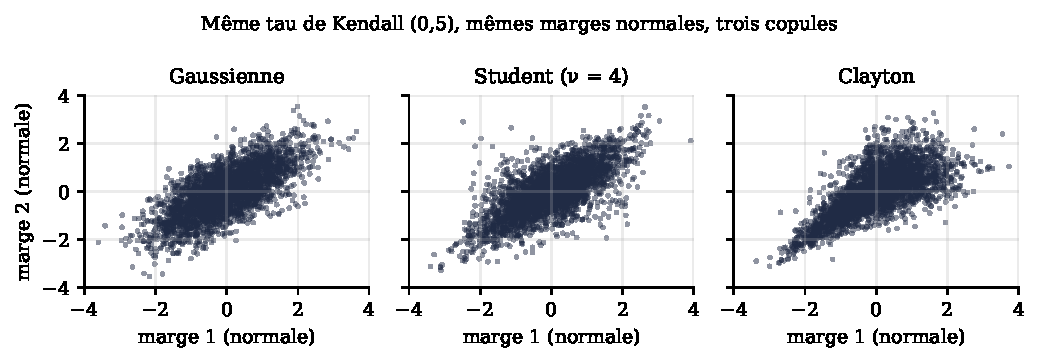
\includegraphics[width=0.98\textwidth]{ch09/trois_copules.pdf}
\caption{Trois copules de même tau de Kendall, représentées avec des marges normales. La Clayton resserre les points dans le coin inférieur gauche (baisses simultanées).}
\label{c9:fig:three}
\end{figure}

\paragraph{Lecture pour le trading.} Une paire couverte avec un ratio estimé en temps normal est exposée à ce qui se passe dans les queues. Si la dépendance de queue est forte, les deux jambes chutent ensemble et la couverture tient ; si elle est faible (une jambe chute seule), l'écart explose. Le choix de la copule est donc d'abord une question de \emph{gestion du risque}.

% =====================================================================
\section{Estimation et choix de la copule}
% =====================================================================

\paragraph{Pseudo-observations.} On ne connaît pas les marges exactes ; on les remplace par les rangs : $\hat u_i = \mathrm{rang}(x_i)/(n+1)$. Diviser par $n+1$ plutôt que $n$ évite les valeurs 0 et 1, où les densités de copule peuvent être infinies.

\paragraph{Paramètre.} Le plus simple est d'inverser la relation entre $\tau$ et le paramètre (tableau~\ref{c9:tab:families}) ; le plus précis est le maximum de vraisemblance sur la densité de copule $c(u,v) = \partial^2C/\partial u\partial v$.

\paragraph{Choix.} On compare les familles par le critère d'Akaike, $\mathrm{AIC} = 2k - 2\ell$, où $k$ est le nombre de paramètres et $\ell$ la log-vraisemblance maximale ; plus petit est meilleur.

\begin{codebox}[ — E2, estimation et choix par AIC]
\textbf{Protocole :} 100 échantillons de 500 observations pour chaque vraie copule ($\tau = 0{,}5$). \textbf{Résultats :} la bonne famille est choisie 98 fois sur 100 (gaussienne), 100 fois (Student), 100 fois (Clayton) ; les paramètres estimés par inversion de $\tau$ valent en moyenne $0{,}710$ (vrai $0{,}707$), $0{,}704$ et $2{,}011$ (vrai $2$).
\end{codebox}

% =====================================================================
\section{Signaux de trading fondés sur les copules}
% =====================================================================

\subsection{La probabilité conditionnelle}

La quantité clé est la \emph{fonction $h$} : $h(u\mid v) = \Prob(U\le u\mid V = v) = \partial C(u,v)/\partial v$. Si $h(u_t\mid v_t)$ est proche de 1, l'actif $X$ a fait \og trop bien\fg{} aujourd'hui compte tenu de ce qu'a fait $Y$ ; proche de 0, trop mal.

\begin{proposition}[Fonction $h$ gaussienne]\label{c9:prop:hgauss}
Pour la copule gaussienne de paramètre $\rho$, $h(u\mid v) = \Phi\Big(\dfrac{\Phi^{-1}(u) - \rho\,\Phi^{-1}(v)}{\sqrt{1-\rho^2}}\Big)$.
\end{proposition}
\begin{proof}
Posons $A = \Phi^{-1}(U)$ et $B = \Phi^{-1}(V)$ : le couple $(A,B)$ est gaussien centré réduit de corrélation $\rho$. D'après le lemme~\ref{c8:lem:cond}, sachant $B = b$, $A$ suit $\N(\rho b, 1-\rho^2)$. Donc $\Prob(U\le u\mid V=v) = \Prob(A\le\Phi^{-1}(u)\mid B = \Phi^{-1}(v)) = \Phi\big((\Phi^{-1}(u)-\rho\Phi^{-1}(v))/\sqrt{1-\rho^2}\big)$.
\end{proof}

Pour Clayton, en dérivant $C$ par rapport à $v$ : $h(u\mid v) = v^{-\theta-1}(u^{-\theta}+v^{-\theta}-1)^{-1/\theta-1}$.

\subsection{Deux règles de la littérature}

\begin{itemize}
\item \citet{liewwu2013} : on calcule chaque jour $h(u_t\mid v_t)$ et $h(v_t\mid u_t)$ sur les rendements ; si la première est inférieure à $0{,}05$ et la seconde supérieure à $0{,}95$, $X$ est jugé sous-évalué par rapport à $Y$ : on achète $X$ et vend $Y$.
\item \citet{xie2016} : on cumule les \og indices de mauvaise évaluation\fg{} $m_t = h(u_t\mid v_t) - 0{,}5$ dans le temps ; on ouvre quand les indices cumulés des deux actifs dépassent un seuil dans des sens opposés et on ferme quand ils reviennent à zéro.
\end{itemize}

\begin{codebox}[ — E3, signal de copule cumulé contre \emph{z-score}]
\textbf{Protocole :} 60 paires simulées, cointégrées en log-prix (écart AR(1), $\varphi = 0{,}9$), chocs de Student à 3 degrés de liberté ; formation de 500 jours (estimation de la copule sur les rendements : la copule de Student est retenue 60 fois sur 60) ; trading de 500 jours ; coûts de 5 pb par jambe. \textbf{Résultats} (gain sur 500 jours, en \% du notionnel brut) : \emph{z-score} sur l'écart $9{,}1\,\%$ (écart-type $4{,}6\,\%$) ; signal de copule cumulé (seuil $0{,}6$) $1{,}6\,\%$ (écart-type $2{,}3\,\%$).
\end{codebox}

\paragraph{Pourquoi la copule fait moins bien ici.} Une copule estimée sur des rendements quotidiens décrit leur dépendance \emph{instantanée}. Si les rendements sont indépendants d'un jour à l'autre, la copule ne contient aucune information sur l'avenir : un \og rendement trop haut\fg{} n'est pas suivi d'une correction. Le signal ne gagne que dans la mesure où l'indice cumulé reconstruit l'écart de niveau, ce que le \emph{z-score} fait directement. \citet{rad2016} trouvent de même que la méthode par copules n'est pas plus rentable que les méthodes par distance et cointégration, même si son profil de risque diffère.

\begin{pitfall}
La copule n'est pas une source de rendement en soi. Elle n'apporte un avantage que si la structure de dépendance contient une information de retour à la moyenne que l'écart linéaire ignore. Son usage le plus robuste est ailleurs : modéliser les co-extrêmes pour dimensionner les positions et placer les stop-loss (chapitre~17).
\end{pitfall}

% =====================================================================
\section{Étude de cas réelle : KO et PEP}
% =====================================================================

\begin{codebox}[ — E4, copule des rendements quotidiens KO/PEP]
Sur 499 rendements quotidiens : $\tau = 0{,}449$. Log-vraisemblances : gaussienne $121{,}4$, Student ($\nu = 4$) $114{,}5$, Clayton $46{,}5$ : l'AIC retient la gaussienne. Jours où les deux titres sont simultanément dans leurs pires 5\,\% : 5 observés, contre 8,6 attendus avec la copule gaussienne ajustée, 10,8 avec la Student, 16,4 avec la Clayton et 1,2 sous indépendance.
\end{codebox}

Sur cette période, les deux titres n'ont pas eu plus de baisses communes extrêmes que ne le prévoit une copule gaussienne. Avec seulement cinq événements, l'incertitude est énorme : un seul épisode de stress aurait pu changer la conclusion. Pour estimer des queues, il faut des historiques longs.

% =====================================================================
\section{Ce que la théorie apporte, et ses limites}
% =====================================================================

\paragraph{Apports.} Séparation propre entre marges et dépendance, mesures de dépendance robustes (rangs), modélisation explicite des co-extrêmes, probabilités conditionnelles interprétables.

\paragraph{Limites.} La copule est statique : elle ne modélise pas la dynamique de retour à la moyenne qui fait gagner un \emph{pairs trade}. Les queues sont estimées sur très peu de points. Le choix de la famille est un a priori fort ; les copules à paramètres variables dans le temps sont plus réalistes mais beaucoup plus difficiles à estimer.

% =====================================================================
\section{Fiche à recopier au tableau blanc}
% =====================================================================

\begin{whiteboard}
\begin{itemize}[leftmargin=1.2em]
\item \textbf{Transformation :} $U = F_X(X)\sim\mathcal U[0,1]$.
\item \textbf{Sklar :} $H(x,y) = C(F_X(x),F_Y(y))$.
\item \textbf{Kendall :} $\tau = \Prob(\text{concordance}) - \Prob(\text{discordance})$ ; gaussienne/Student : $\rho = \sin(\pi\tau/2)$ ; Clayton : $\theta = 2\tau/(1-\tau)$.
\item \textbf{Queue :} $\lambda_L = \lim_{q\to0}\Prob(V\le q\mid U\le q)$ ; Clayton $2^{-1/\theta}$ ; gaussienne 0.
\item \textbf{Clayton :} $C = (u^{-\theta}+v^{-\theta}-1)^{-1/\theta}$.
\item \textbf{Fonction $h$ :} $h(u|v) = \partial C/\partial v$ ; gaussienne $\Phi\big((\Phi^{-1}(u)-\rho\Phi^{-1}(v))/\sqrt{1-\rho^2}\big)$.
\item \textbf{Pseudo-observations :} rang$/(n+1)$ ; choix par AIC $= 2k-2\ell$.
\end{itemize}
\end{whiteboard}

% =====================================================================
\section{Exercices}
% =====================================================================

\begin{exercise}
Montrez que la copule d'indépendance est $C(u,v) = uv$ et que son tau de Kendall est nul.
\end{exercise}

\begin{exercise}
Démontrez la formule $\lambda_L = 2^{-1/\theta}$ pour la copule de Clayton en calculant $C(q,q)/q$ et en faisant tendre $q$ vers 0.
\end{exercise}

\begin{exercise}
Dérivez la fonction $h$ de la copule de Clayton à partir de $C(u,v)$.
\end{exercise}

\begin{exercise}[à coder]
Ajoutez la copule de Clayton \og tournée\fg{} (de survie) $\tilde C(u,v) = u + v - 1 + C(1-u,1-v)$, qui a une dépendance de queue supérieure. Mesurez sur KO/PEP si elle améliore l'AIC.
\end{exercise}

\begin{exercise}[à coder]
Modifiez E3 pour que les rendements simulés aient une composante prévisible (par exemple une réaction partielle de $X$ aux chocs de $Y$ du jour précédent). La copule estimée sur les couples $(r^X_{t+1}, r^Y_t)$ fait-elle alors mieux que le \emph{z-score} ?
\end{exercise}

% =====================================================================
\section{Pour aller plus loin}
% =====================================================================

\begin{toread}
\begin{itemize}[leftmargin=1.2em]
\item \citet{liewwu2013} : la première application des copules au \emph{pairs trading}, avec la règle des probabilités conditionnelles.
\item \citet{xie2016} : l'indice de mauvaise évaluation cumulé.
\item \citet{rad2016} : la comparaison de la méthode par copules avec les méthodes par distance et cointégration sur longue période.
\item \citet{krauss2017survey}, partie consacrée aux \og autres approches\fg{} : synthèse des variantes à base de copules.
\end{itemize}
\end{toread}

\section{Scripts du chapitre}
\noindent\texttt{code/ch09/ch09\_copulas.py} : E1 (figure~\ref{c9:fig:three}), E2, E3, E4.

% =====================================================================
\chapter{Arbitrage statistique multi-actifs}
\label{ch:10}
% =====================================================================

\section{Objectifs et organisation du chapitre}

\paragraph{Objectifs.} Une paire est un cas particulier : on couvre une action par une autre. Plus généralement, on peut couvrir chaque action par les facteurs communs à tout le marché et trader ce qui reste, son \emph{résidu}. C'est l'approche d'\citet{avellaneda2010}, qui a structuré l'arbitrage statistique institutionnel sur actions. À la fin du chapitre, vous saurez : (1) dériver l'analyse en composantes principales (ACP) et construire des portefeuilles propres ; (2) distinguer les vrais facteurs du bruit d'estimation (borne de Marchenko-Pastur) ; (3) modéliser les résidus par un processus d'Ornstein-Uhlenbeck et calculer le \emph{s-score} ; (4) implémenter et tester la stratégie complète ; (5) situer les approches de portefeuilles de retour à la moyenne parcimonieux.

\paragraph{Code.} \texttt{code/ch10/ch10\_pca\_statarb.py}.

% =====================================================================
\section{L'analyse en composantes principales}
% =====================================================================

\subsection{Le problème}

Soit $C$ la matrice de corrélation des rendements standardisés de $N$ actions ($N\times N$, symétrique, positive). On cherche la combinaison $w$ (de norme 1) dont la variance $w^\top Cw$ est maximale : la direction qui explique le plus de mouvements communs.

\begin{proposition}\label{c10:prop:pca}
Le maximum de $w^\top Cw$ sous la contrainte $w^\top w = 1$ est atteint en $w = v_1$, vecteur propre associé à la plus grande valeur propre $\lambda_1$ de $C$, et vaut $\lambda_1$. Les composantes suivantes sont les vecteurs propres suivants, orthogonaux entre eux.
\end{proposition}
\begin{proof}
On introduit un multiplicateur de Lagrange $\lambda$ et l'on annule le gradient de $w^\top Cw - \lambda(w^\top w - 1)$ : $2Cw - 2\lambda w = 0$, soit $Cw = \lambda w$. Les candidats sont donc les vecteurs propres de $C$, et pour un tel vecteur la variance vaut $w^\top Cw = \lambda w^\top w = \lambda$. Le maximum est atteint pour la plus grande valeur propre. Pour la deuxième composante, on ajoute la contrainte d'orthogonalité à $v_1$ et le même raisonnement donne $v_2$.
\end{proof}

La somme des valeurs propres vaut $\mathrm{tr}(C) = N$ ; la part de variance expliquée par les $k$ premières composantes est $\sum_{j\le k}\lambda_j/N$. Sur les actions, la première composante est presque toujours le \og marché\fg{} (tous les poids de même signe), les suivantes opposent des secteurs ou des styles.

\paragraph{Portefeuilles propres.} Les vecteurs propres portent sur des rendements standardisés ; pour obtenir un portefeuille investissable, on divise chaque poids par la volatilité de l'action : $Q_{ij} = v_{j,i}/\sigma_i$. Le rendement du facteur $j$ est $F_{jt} = \sum_iQ_{ij}R_{it}$.

\subsection{Combien de facteurs ? La borne de Marchenko-Pastur}

Même si les actions étaient indépendantes, la matrice de corrélation estimée sur $T$ jours aurait des valeurs propres dispersées autour de 1, par pur bruit d'échantillonnage. La théorie des matrices aléatoires montre que, pour des séries indépendantes et $N/T = q$ fixé, les valeurs propres se répartissent entre $(1-\sqrt q)^2$ et $(1+\sqrt q)^2$. Une valeur propre au-dessus de $(1+\sqrt q)^2$ signale un facteur réel ; celles en dessous sont indiscernables du bruit.

\begin{codebox}[ — E1, spectre et borne de Marchenko-Pastur]
\textbf{Protocole :} 100 actions simulées avec 3 facteurs, fenêtre de 252 jours ($q = 0{,}40$, borne $2{,}66$). \textbf{Résultats :} valeurs propres $29{,}7$ ; $10{,}4$ ; $6{,}8$ ; puis $1{,}42$ ; $1{,}39$\dots{} Exactement trois valeurs propres dépassent la borne ; elles expliquent 47\,\% de la variance.
\end{codebox}

\begin{figure}[h]
\centering
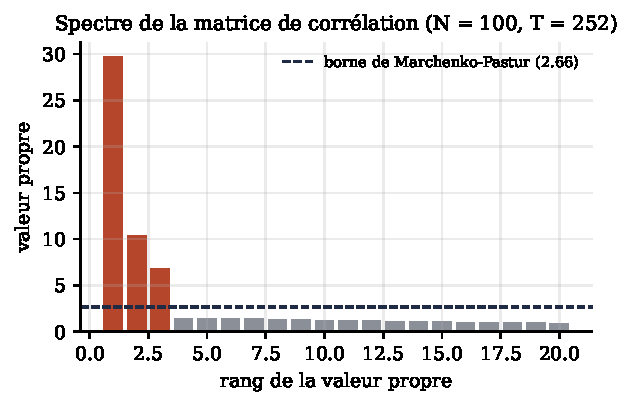
\includegraphics[width=0.62\textwidth]{ch10/spectre_valeurs_propres.pdf}
\caption{Les 20 plus grandes valeurs propres de la matrice de corrélation ; en rouge, celles qui dépassent la borne de Marchenko-Pastur.}
\label{c10:fig:spectrum}
\end{figure}

% =====================================================================
\section{Le modèle d'Avellaneda et Lee}
% =====================================================================

\subsection{Décomposition des rendements}

Chaque action suit
\[
\frac{\dd P_{it}}{P_{it}} = \alpha_i\,\dd t + \sum_{j=1}^{k}\beta_{ij}\,F_{jt}\,\dd t + \dd X_{it},
\]
où les $F_j$ sont les rendements des facteurs (portefeuilles propres ou ETF sectoriels) et $X_{it}$ est le \emph{résidu cumulé}, supposé suivre un processus d'Ornstein-Uhlenbeck (chapitre~5) : $\dd X_{it} = \kappa_i(m_i - X_{it})\dd t + \sigma_i\dd W_{it}$. Une position longue sur l'action et courte sur $\beta_{ij}$ unités de chaque facteur n'est exposée qu'à $X_{it}$.

\begin{intuition}
Chaque action est un passager dans un bus (le marché) qui roule vite et change de direction. Le chauffeur, c'est le facteur ; on ne sait pas où il va. Mais chaque passager se déplace aussi dans l'allée, et il finit toujours par revenir à sa place. On ne parie pas sur la route du bus ; on parie que le passager qui est trop loin de sa place va y retourner.
\end{intuition}

\subsection{Estimation, pas à pas}

Chaque jour $t$ :
\begin{enumerate}
\item \textbf{Facteurs :} ACP sur la matrice de corrélation des 252 derniers jours ; on garde $k$ portefeuilles propres.
\item \textbf{Régression :} pour chaque action, régression de ses rendements des 60 derniers jours sur ceux des facteurs ; on obtient $\hat\beta_{ij}$ et les résidus $\hat\varepsilon_{is}$.
\item \textbf{Résidu cumulé :} $X_{is} = \sum_{u\le s}\hat\varepsilon_{iu}$ sur la fenêtre.
\item \textbf{AR(1) :} $X_{i,s+1} = a_i + b_iX_{is} + \zeta_{i,s+1}$ ; d'où, par la correspondance du chapitre~5, $\kappa_i = -252\ln b_i$, $m_i = a_i/(1-b_i)$ et $\sigma_{eq,i} = \sqrt{\Var(\zeta_i)/(1-b_i^2)}$.
\item \textbf{s-score :} $s_i = (X_{it} - m_i)/\sigma_{eq,i}$ : l'écart actuel du résidu à son équilibre, en écarts-types stationnaires.
\end{enumerate}

\subsection{Règles de trading}

Avellaneda et Lee utilisent des seuils asymétriques : ouvrir une position courte si $s_i > 1{,}25$ et longue si $s_i < -1{,}25$ ; fermer la position courte quand $s_i < 0{,}75$ et la longue quand $s_i > -0{,}5$. Ils ne tradent que les actions dont le retour est assez rapide : $\kappa_i > 252/30$, soit un temps caractéristique $1/\kappa_i$ inférieur à environ 30 jours de bourse, une demi-vie inférieure à une vingtaine de jours. Chaque position est couverte par les facteurs, de sorte que le portefeuille est proche de la neutralité au marché.

\paragraph{Résultats publiés.} Selon le résumé de l'article, la version ACP affiche un ratio de Sharpe annuel moyen de $1{,}44$ sur 1997–2007 sur les actions américaines, avec une performance plus forte avant 2003 ; l'ajout d'une information de volume améliore les résultats.

% =====================================================================
\section{Expérience}
% =====================================================================

\begin{codebox}[ — E2 et E3, stratégie s-score sur univers simulé]
\textbf{Protocole :} 100 actions, 3 facteurs, 1\,000 jours de trading. Scénario \og signal\fg{} : résidus cumulés OU de demi-vie 8 jours (écart-type stationnaire 3\,\%) plus un bruit quotidien ; scénario \og nul\fg{} : résidus en bruit blanc de même variance quotidienne. \textbf{Résultats} (rendement annuel ; ratio de Sharpe) :
\begin{center}\small
\begin{tabular}{lccc}
\toprule
 & 0 pb & 5 pb & 10 pb\\
\midrule
Signal, $k = 1$ facteur & $9{,}1\,\%$ ; 4,1 & $8{,}2\,\%$ ; 3,7 & $7{,}3\,\%$ ; 3,3\\
Signal, $k = 3$ facteurs & $10{,}5\,\%$ ; 9,0 & $9{,}6\,\%$ ; 8,2 & $8{,}6\,\%$ ; 7,4\\
Signal, $k = 10$ facteurs & $10{,}1\,\%$ ; 8,4 & $9{,}0\,\%$ ; 7,5 & $8{,}0\,\%$ ; 6,7\\
Nul, $k = 3$ & $-0{,}1\,\%$ ; $-0{,}1$ & $-1{,}0\,\%$ ; $-0{,}8$ & $-1{,}9\,\%$ ; $-1{,}4$\\
\bottomrule
\end{tabular}
\end{center}
\end{codebox}

\begin{figure}[h]
\centering
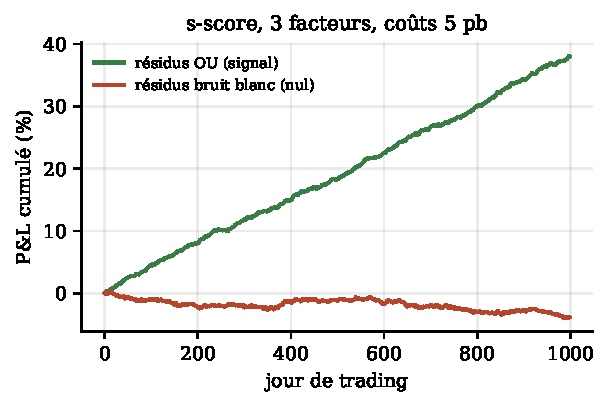
\includegraphics[width=0.62\textwidth]{ch10/pnl_sscore.pdf}
\caption{P\&L cumulé de la stratégie s-score (3 facteurs, 5 pb) quand les résidus reviennent à la moyenne et quand ils ne le font pas.}
\label{c10:fig:pnl}
\end{figure}

\paragraph{Lecture.} (1) Avec un seul facteur, une partie du risque sectoriel reste dans les résidus : la volatilité double et le Sharpe est divisé par deux. Avec trop de facteurs (10 au lieu de 3), on retire un peu de signal avec le bruit. Le bon nombre est celui que suggère Marchenko-Pastur. (2) Sans retour à la moyenne des résidus, la méthode ne gagne rien et perd ses coûts : elle ne crée pas d'avantage, elle l'exploite. (3) Les Sharpe de 8 du monde simulé sont irréalistes : le modèle y est exactement vrai, les paramètres constants, l'exécution parfaite. La valeur publiée de $1{,}44$, en déclin, donne l'ordre de grandeur réel.

\begin{pitfall}
Cette stratégie fait beaucoup de transactions sur beaucoup de titres : les coûts, l'impact et le coût d'emprunt des titres vendus à découvert y sont déterminants. Elle est aussi typiquement \og encombrée\fg : lors de la crise d'août 2007, de nombreux fonds détenant des portefeuilles semblables ont dû liquider en même temps \citep{khandanilo2011}. Pour un particulier, l'univers doit rester restreint aux titres très liquides et faciles à emprunter.
\end{pitfall}

% =====================================================================
\section{Portefeuilles de retour à la moyenne parcimonieux}
% =====================================================================

Plutôt que de couvrir chaque action par des facteurs, on peut chercher directement la combinaison d'actifs la plus prévisible. \citet{boxtiao1977} posent le problème pour un VAR(1) $x_t = Ax_{t-1} + \varepsilon_t$ : la prévisibilité d'un portefeuille $w$ est le rapport entre la variance de sa partie prévue et sa variance totale, $\lambda(w) = w^\top A\Gamma A^\top w/w^\top\Gamma w$ (avec $\Gamma$ la covariance de $x$). Minimiser $\lambda$ donne le portefeuille qui revient le plus vite à la moyenne ; c'est un problème de valeur propre généralisée, de même nature que la proposition~\ref{c10:prop:pca}. \citet{daspremont2011} ajoute une contrainte de parcimonie (peu d'actifs non nuls) pour obtenir des portefeuilles tradables à faibles coûts.

% =====================================================================
\section{Ce que la théorie apporte, et ses limites}
% =====================================================================

\paragraph{Apports.} Une généralisation naturelle du \emph{pairs trading} à tout un univers, une neutralisation explicite des risques communs, un critère objectif du nombre de facteurs, et un signal (le \emph{s-score}) directement issu du modèle OU.

\paragraph{Limites.} Facteurs instables d'une fenêtre à l'autre (les vecteurs propres peuvent changer de signe ou d'ordre) ; estimation sur 60 jours très bruitée ; coûts élevés ; profits historiques en déclin ; risque de foule. L'approche demande une infrastructure de données et d'exécution plus lourde que le \emph{pairs trading} simple.

% =====================================================================
\section{Fiche à recopier au tableau blanc}
% =====================================================================

\begin{whiteboard}
\begin{itemize}[leftmargin=1.2em]
\item \textbf{ACP :} $\max_w w^\top Cw$ s.c. $w^\top w=1$ $\Rightarrow$ $Cw = \lambda w$ ; part expliquée $\sum_{j\le k}\lambda_j/N$.
\item \textbf{Portefeuille propre :} $Q_{ij} = v_{j,i}/\sigma_i$, $F_{jt} = \sum_iQ_{ij}R_{it}$.
\item \textbf{Marchenko-Pastur :} bruit entre $(1\pm\sqrt{N/T})^2$.
\item \textbf{Modèle :} $R_i = \alpha_i + \sum_j\beta_{ij}F_j + \dd X_i$, $X_i$ OU.
\item \textbf{AR(1) sur $X$ :} $\kappa = -252\ln b$, $m = a/(1-b)$, $\sigma_{eq} = \sqrt{\Var(\zeta)/(1-b^2)}$.
\item \textbf{s-score :} $s = (X - m)/\sigma_{eq}$ ; ouvrir à $\pm1{,}25$, fermer court à $0{,}75$, long à $-0{,}5$ ; filtre $\kappa > 252/30$.
\item \textbf{Box-Tiao :} minimiser $w^\top A\Gamma A^\top w/w^\top\Gamma w$.
\end{itemize}
\end{whiteboard}

% =====================================================================
\section{Exercices}
% =====================================================================

\begin{exercise}
Montrez que deux vecteurs propres d'une matrice symétrique associés à des valeurs propres distinctes sont orthogonaux. Pourquoi les rendements des portefeuilles propres sont-ils alors non corrélés sur la fenêtre d'estimation ?
\end{exercise}

\begin{exercise}
Calculez la borne de Marchenko-Pastur pour 500 actions et 252 jours, puis pour 500 actions et 1\,000 jours. Commentez.
\end{exercise}

\begin{exercise}
Avec $b = 0{,}9$ sur données quotidiennes, calculez $\kappa$ et la demi-vie. Le titre passe-t-il le filtre d'Avellaneda et Lee ?
\end{exercise}

\begin{exercise}[à coder]
Remplacez les portefeuilles propres par un seul facteur \og marché\fg{} égal à la moyenne des rendements et comparez avec $k = 1$ en ACP.
\end{exercise}

\begin{exercise}[données réelles]
Construisez un univers de 30 à 50 ETF ou actions très liquides (via Interactive Brokers) et calculez le spectre de leur matrice de corrélation sur un an. Combien de valeurs propres dépassent la borne ?
\end{exercise}

% =====================================================================
\section{Pour aller plus loin}
% =====================================================================

\begin{toread}
\begin{itemize}[leftmargin=1.2em]
\item \citet{avellaneda2010} : la section sur la construction des facteurs (ACP et ETF), celle sur le \emph{s-score} et l'annexe sur l'estimation des paramètres OU.
\item \citet{boxtiao1977} et \citet{daspremont2011} : portefeuilles de retour à la moyenne.
\item \citet{khandanilo2011} : ce qui arrive quand tout le monde trade la même chose.
\item \citet{guijarro2021} : la version \og apprentissage profond\fg{} des signaux sur résidus, reprise au chapitre~11.
\end{itemize}
\end{toread}

\section{Scripts du chapitre}
\noindent\texttt{code/ch10/ch10\_pca\_statarb.py} : E1 (figure~\ref{c10:fig:spectrum}), E2–E3 (figure~\ref{c10:fig:pnl}).

% =====================================================================
\chapter{Apprentissage automatique}
\label{ch:11}
% =====================================================================

\section{Objectifs et organisation du chapitre}

\paragraph{Objectifs.} L'apprentissage automatique promet de découvrir des relations non linéaires que les modèles des chapitres précédents ignorent. Il promet aussi, et surtout, de se tromper avec une assurance remarquable. À la fin de ce chapitre, vous saurez : (1) situer les usages de l'apprentissage automatique en arbitrage statistique ; (2) construire variables explicatives et étiquettes sans information future ; (3) reconnaître et éviter la fuite d'information en validation croisée ; (4) comparer honnêtement un modèle complexe à une règle simple ; (5) utiliser la réduction de dimension et le \emph{clustering} pour sélectionner des paires.

\paragraph{Code.} \texttt{code/ch11/ch11\_machine\_learning.py} (\texttt{scikit-learn}).

% =====================================================================
\section{Trois usages}
% =====================================================================

\begin{enumerate}
\item \textbf{Prévoir les rendements relatifs.} \citet{krauss2017ml} entraînent chaque jour des réseaux profonds, du \emph{gradient boosting} et des forêts aléatoires à prédire quelles actions du S\&P~500 surperformeront la médiane le lendemain, à partir des rendements passés ; ils achètent les mieux classées et vendent les moins bien classées. L'ensemble des modèles produit, selon les auteurs, environ $0{,}45\,\%$ par jour avant coûts sur 1992–2015, avec un net déclin dans la période récente.
\item \textbf{Extraire des signaux des résidus.} \citet{guijarro2021} appliquent des réseaux convolutifs et des \emph{transformers} aux trajectoires de résidus (au sens du chapitre~10) pour apprendre directement la règle de trading, et rapportent des ratios de Sharpe hors échantillon élevés.
\item \textbf{Sélectionner les paires.} \citet{sarmento2020} réduisent la dimension des rendements par ACP, regroupent les actions par un algorithme de \emph{clustering} (OPTICS), puis appliquent les tests de cointégration à l'intérieur des groupes.
\end{enumerate}

% =====================================================================
\section{Variables, étiquettes et fuite d'information}
% =====================================================================

\subsection{Variables et étiquettes}

Une \emph{variable explicative} (\emph{feature}) $f_t$ doit être calculable avec l'information disponible à la date $t$ : rendements passés, \emph{z-score} de l'écart, volatilité récente, demi-vie estimée. Une \emph{étiquette} (\emph{label}) $y_t$ décrit ce qu'on veut prévoir et regarde par définition vers l'avenir : signe du rendement de l'écart sur les $H$ prochains jours, ou résultat d'un trade (gain, perte, expiration) selon la méthode des trois barrières de \citet{lopezdeprado2018}.

\subsection{Le problème du chevauchement}

Si l'étiquette porte sur $H > 1$ jours, les étiquettes de deux dates voisines partagent $H-1$ jours de rendements futurs : $y_t$ et $y_{t+1}$ sont presque identiques. Une validation croisée classique (\emph{K-fold}) qui mélange les dates place des dates voisines à la fois dans l'apprentissage et dans le test. Le modèle \og reconnaît\fg{} la période et recopie l'étiquette de la date voisine : il paraît prévoir, alors qu'il se souvient.

\begin{intuition}
C'est comme préparer un examen avec les corrigés de la veille d'une épreuve dont la moitié des questions sont reprises le lendemain. Votre note sera excellente, et ne dira rien de votre capacité à résoudre une question nouvelle.
\end{intuition}

\paragraph{Le remède : validation séquentielle purgée.} On entraîne toujours sur le passé et on teste sur le futur (\emph{walk-forward}) ; on \emph{purge} de l'apprentissage les dates dont les étiquettes chevauchent la période de test, et l'on ajoute un \emph{embargo} de quelques jours après le test \citep{lopezdeprado2018}.

\begin{codebox}[ — E1, fuite d'information]
\textbf{Protocole :} 10 marches aléatoires de 3\,000 jours (\emph{aucune} prévisibilité) ; six variables passées (rendements sur 1, 5, 10, 20 jours, \emph{z-score} sur 20 jours, volatilité) ; étiquette : signe du rendement sur les 10 jours suivants ; forêt aléatoire de 200 arbres. \textbf{Résultats :} précision en validation croisée mélangée à 5 blocs : $58{,}4\,\%$ en moyenne (de $54{,}7$ à $60{,}7\,\%$) ; en validation séquentielle purgée : $50{,}7\,\%$ (de $46{,}4$ à $55{,}0\,\%$). La vraie précision possible est $50\,\%$.
\end{codebox}

\begin{pitfall}
Une précision de 58\,\% en validation croisée ressemble à une découverte majeure : avec un ratio gain/perte de 1, elle donnerait un ratio de Sharpe considérable. Elle est entièrement due à la fuite d'information. Toute étude d'apprentissage automatique en finance qui ne précise pas comment elle a évité le chevauchement doit être considérée comme fausse jusqu'à preuve du contraire.
\end{pitfall}

% =====================================================================
\section{Complexe contre simple}
% =====================================================================

Quand la structure du signal est connue et linéaire (un écart qui revient à la moyenne), un modèle flexible doit au mieux redécouvrir la règle simple, avec plus de variance.

\begin{codebox}[ — E2, forêt aléatoire contre règle \emph{z-score}]
\textbf{Protocole :} 10 écarts simulés (AR(1) avec $\varphi = 0{,}95$ plus une petite marche aléatoire), 4\,000 jours, apprentissage sur la première moitié, test sur la seconde ; étiquette : signe du rendement du lendemain ; position de la forêt si la probabilité prédite sort de $[0{,}45\,;\,0{,}55]$ ; règle simple : \emph{z-score} à 20 jours au-delà de $\pm1$ ; coûts de 1 pb. \textbf{Résultats :} taux de réussite $53{,}3\,\%$ (forêt) contre $53{,}5\,\%$ (règle) ; P\&L moyen $0{,}54$ contre $0{,}87$ (en unités de l'écart).
\end{codebox}

La forêt n'apporte rien et perd une partie du signal : elle doit apprendre à partir de bruit ce que la règle encode directement. L'apprentissage automatique n'a d'intérêt que s'il existe une structure que les modèles simples ne capturent pas (interactions entre variables, non-linéarités, informations hétérogènes comme les volumes ou le carnet d'ordres), \emph{et} assez de données pour l'apprendre.

\paragraph{Bonnes pratiques.} Comparer systématiquement à une règle simple de référence ; préférer des modèles peu profonds et fortement régularisés ; compter toutes les variantes essayées (chapitre~16) ; mesurer l'importance des variables sur l'échantillon de test ; ré-entraîner à intervalles réguliers en walk-forward, jamais sur l'échantillon complet.

% =====================================================================
\section{Sélection de paires par \emph{clustering}}
% =====================================================================

\subsection{La méthode}

Le chapitre~7 a montré que tester toutes les paires coûte cher en faux positifs. L'idée de \citet{sarmento2020} : réduire d'abord l'univers à des groupes d'actions qui se ressemblent, puis tester seulement à l'intérieur des groupes.
\begin{enumerate}
\item On standardise les rendements et l'on fait une ACP : chaque action est représentée par ses coordonnées sur les $k$ premières composantes (ses \og expositions\fg{} aux facteurs).
\item On regroupe les actions proches dans cet espace avec OPTICS, un algorithme qui détecte des groupes de densité variable et laisse de côté les points isolés.
\item On teste la cointégration (avec correction BH) uniquement pour les paires d'un même groupe.
\end{enumerate}

\begin{codebox}[ — E3, ACP + OPTICS + cointégration]
\textbf{Protocole :} univers simulé du chapitre~7 (100 actions, 10 vraies paires de demi-vie 4,3 jours), 500 jours ; 8 composantes ; OPTICS avec \texttt{min\_samples = 2}. \textbf{Résultats} (4 univers) : 27 à 31 groupes ; 57 à 93 paires candidates au lieu de 4\,950 ; les 10 vraies paires sont toujours parmi les candidates ; après BH, 10 ou 11 paires retenues dont les 10 vraies.
\end{codebox}

Le \emph{clustering} divise le nombre de tests par 50 à 80 sans perdre les vraies paires, ce qui rend la correction pour tests multiples beaucoup moins coûteuse en puissance. Dans cette simulation, les deux actions d'une vraie paire ont exactement les mêmes expositions aux facteurs, ce qui les rend faciles à regrouper ; sur données réelles, les groupes sont moins nets et le résultat doit être vérifié.

% =====================================================================
\section{Ce que la théorie apporte, et ses limites}
% =====================================================================

\paragraph{Apports.} Des modèles capables d'exploiter des structures non linéaires et des données hétérogènes ; des outils de réduction de dimension et de regroupement qui structurent la recherche de paires ; une discipline de validation (purge, embargo, walk-forward) utile à toute stratégie.

\paragraph{Limites.} Rapport signal/bruit très faible des rendements financiers ; non-stationnarité (ce qui a été appris peut ne plus valoir) ; risque de surapprentissage démultiplié par le nombre d'hyperparamètres ; résultats publiés obtenus sur des univers très liquides, avec des coûts que le particulier ne peut pas toujours égaler ; opacité qui complique le diagnostic quand la stratégie se dégrade.

% =====================================================================
\section{Fiche à recopier au tableau blanc}
% =====================================================================

\begin{whiteboard}
\begin{itemize}[leftmargin=1.2em]
\item \textbf{Variable :} calculable en $t$ ; \textbf{étiquette :} regarde vers $t+H$.
\item \textbf{Chevauchement :} étiquettes à horizon $H$ partagent $H-1$ jours $\Rightarrow$ K-fold mélangé fuit.
\item \textbf{Remède :} walk-forward, purge des dates qui chevauchent le test, embargo.
\item \textbf{Test de base :} toujours comparer à une règle simple sur le même échantillon de test.
\item \textbf{Sélection :} ACP (expositions) $\to$ OPTICS (groupes) $\to$ cointégration intra-groupe $+$ BH.
\end{itemize}
\end{whiteboard}

% =====================================================================
\section{Exercices}
% =====================================================================

\begin{exercise}
Avec une étiquette à horizon $H = 10$ et 2\,500 dates, combien de dates faut-il purger autour d'un bloc de test de 250 dates ? Quelle fraction des données d'apprentissage perd-on par bloc ?
\end{exercise}

\begin{exercise}
Expliquez pourquoi une forêt aléatoire dont les feuilles contiennent une seule observation (\texttt{min\_samples\_leaf = 1}) amplifie la fuite d'information de E1.
\end{exercise}

\begin{exercise}[à coder]
Refaites E1 avec \texttt{min\_samples\_leaf = 200}. La précision de la validation mélangée baisse-t-elle ? Disparaît-elle ?
\end{exercise}

\begin{exercise}[à coder]
Dans E2, ajoutez une non-linéarité réelle : le retour à la moyenne n'existe que quand la volatilité récente est basse. La forêt bat-elle alors la règle simple ? Avec combien de données ?
\end{exercise}

\begin{exercise}[données réelles]
Appliquez la méthode ACP + OPTICS à un univers d'une cinquantaine d'actions de deux ou trois secteurs. Les groupes trouvés correspondent-ils aux secteurs ?
\end{exercise}

% =====================================================================
\section{Pour aller plus loin}
% =====================================================================

\begin{toread}
\begin{itemize}[leftmargin=1.2em]
\item \citet{lopezdeprado2018}, chapitres~3 (étiquetage, méthode des trois barrières), 4 (pondération des échantillons qui se chevauchent) et 7 (validation croisée purgée).
\item \citet{krauss2017ml} : protocole complet de prévision quotidienne sur le S\&P~500.
\item \citet{guijarro2021} : signaux appris sur les résidus d'arbitrage statistique.
\item \citet{sarmento2020} : la sélection de paires par ACP et OPTICS.
\end{itemize}
\end{toread}

\section{Scripts du chapitre}
\noindent\texttt{code/ch11/ch11\_machine\_learning.py} : E1 (fuite d'information), E2 (forêt contre règle), E3 (\emph{clustering}).


\part{Arbitrage inter-plateformes}
% =====================================================================
\chapter{Microstructure et coûts de transaction}
\label{ch:12}
% =====================================================================

\section{Objectifs et organisation du chapitre}

\paragraph{Objectifs.} Les parties I et II ont montré qu'un avantage d'arbitrage statistique se mesure en points de base. Cette partie descend au niveau où ces points de base se gagnent ou se perdent : le carnet d'ordres. À la fin du chapitre, vous saurez : (1) décrire un carnet d'ordres et la différence entre ordres \emph{maker} et \emph{taker} ; (2) estimer une fourchette à partir des prix (estimateur de Roll) et connaître ses limites ; (3) construire un modèle de coût complet pour un aller-retour de paire ; (4) en déduire l'amplitude minimale d'un écart tradable ; (5) mesurer l'effet des hypothèses d'exécution sur un \emph{backtest} ; (6) estimer l'ordre de grandeur de l'impact de marché \citep{harris2003}.

\paragraph{Code.} \texttt{code/ch12/ch12\_microstructure.py}.

% =====================================================================
\section{Le carnet d'ordres}
% =====================================================================

\subsection{Vocabulaire}

Un marché électronique centralise des \emph{ordres limites} : des intentions d'acheter (\emph{bid}) ou de vendre (\emph{ask}) une quantité à un prix maximal ou minimal. Le meilleur prix acheteur et le meilleur prix vendeur forment le \og haut du carnet\fg ; leur différence est la \emph{fourchette} (\emph{spread}), leur moyenne le \emph{prix milieu} (\emph{mid}). La quantité disponible à chaque prix est la \emph{profondeur}.

\begin{itemize}
\item Un ordre \textbf{taker} (ordre au marché, ou ordre limite qui croise le carnet) s'exécute immédiatement contre les ordres en attente : il \og prend\fg{} la liquidité et paie la demi-fourchette.
\item Un ordre \textbf{maker} (ordre limite qui ne croise pas) attend dans le carnet : il \og fournit\fg{} la liquidité, n'est exécuté que si quelqu'un vient le chercher, et reçoit souvent une remise ou paie des frais plus faibles. Un ordre \emph{post-only} est rejeté s'il devait s'exécuter immédiatement, ce qui garantit le statut de maker.
\end{itemize}

\begin{intuition}
Le carnet est un marché aux puces. Le taker est pressé : il achète au prix affiché par le vendeur. Le maker affiche son prix et attend ; il obtient un meilleur prix, mais il n'est pas sûr d'être servi, et il l'est le plus souvent quand le marché bouge contre lui (le passant qui accepte votre prix d'achat sait peut-être que le prix va baisser). C'est la \emph{sélection adverse}, au cœur du chapitre~15.
\end{intuition}

\subsection{Les composantes du coût}

Pour une transaction de notionnel $N$, le coût total se décompose en :
\begin{enumerate}
\item \textbf{commissions et frais} de la plateforme ou du courtier (fixes, par action, ou en points de base ; maker et taker différenciés) ;
\item \textbf{demi-fourchette} payée par un ordre taker ;
\item \textbf{impact de marché} : un ordre important consomme plusieurs niveaux du carnet et déplace le prix ;
\item \textbf{glissement} (\emph{slippage}) : écart entre le prix observé au moment de la décision et le prix d'exécution, dû à la latence ;
\item \textbf{coûts de portage} : emprunt des titres vendus à découvert, financement de la marge, \emph{funding} des contrats perpétuels (chapitre~14).
\end{enumerate}

% =====================================================================
\section{Estimer la fourchette : l'estimateur de Roll}
% =====================================================================

Supposons que le prix milieu $m_t$ suive une marche aléatoire et que chaque transaction ait lieu au prix acheteur ou vendeur avec la même probabilité : $p_t = m_t + \frac s2 q_t$, où $q_t = \pm1$ est indépendant de tout le reste et $s$ la fourchette.

\begin{proposition}[Roll]\label{c12:prop:roll}
Sous ces hypothèses, $\Cov(\Delta p_t,\Delta p_{t-1}) = -s^2/4$, donc $s = 2\sqrt{-\Cov(\Delta p_t,\Delta p_{t-1})}$.
\end{proposition}
\begin{proof}
$\Delta p_t = \Delta m_t + \frac s2(q_t - q_{t-1})$. Les variations du prix milieu sont indépendantes entre elles et des $q$, donc
\[
\Cov(\Delta p_t,\Delta p_{t-1}) = \frac{s^2}4\Cov(q_t - q_{t-1},\, q_{t-1} - q_{t-2}) = \frac{s^2}4\big(0 - 0 - \Var(q_{t-1}) + 0\big) = -\frac{s^2}4,
\]
car seuls les termes en $q_{t-1}$ sont corrélés et $\Var(q_{t-1}) = 1$.
\end{proof}

L'intuition : le prix \og rebondit\fg{} entre acheteur et vendeur, ce qui crée une autocorrélation négative des variations successives.

\begin{codebox}[ — E1, estimateur de Roll]
\textbf{Simulation} (200\,000 transactions) : fourchettes vraies de 2, 10 et 50 pb, estimées à $2{,}1$ ; $10{,}1$ et $47{,}4$ pb. \textbf{Clôtures quotidiennes réelles} : l'estimateur donne $66$ pb pour GLD, $62$ pour GLDM, $41$ pour KO et $50$ pour PEP, alors que les fourchettes réelles de ces titres très liquides se mesurent en points de base unitaires.
\end{codebox}

\begin{pitfall}
Sur des données quotidiennes, l'autocorrélation négative des rendements a d'autres causes que le rebond acheteur-vendeur (corrections, nouvelles absorbées sur plusieurs jours) et l'estimateur de Roll n'a plus de sens. Les coûts doivent être mesurés sur données de transaction, ou mieux, sur vos propres exécutions : le prix obtenu comparé au prix milieu au moment de la décision.
\end{pitfall}

% =====================================================================
\section{Le coût d'un aller-retour de paire}
% =====================================================================

Un trade de paire comprend quatre transactions : achat et vente de chaque jambe, à l'entrée puis à la sortie. Si chaque transaction coûte $c$ points de base (commission, demi-fourchette, impact), l'aller-retour coûte $4c$ en points de base du notionnel d'une jambe, plus le coût d'emprunt sur la durée de détention.

Le chapitre~1 a établi qu'un aller-retour entre $\pm2\sigma_{eq}$ et 0 capture environ $2\sigma_{eq}$. Exiger que ce gain couvre au moins deux fois les coûts donne une règle simple : \textbf{l'écart-type stationnaire de l'écart doit être au moins égal au coût total d'un aller-retour}.

\begin{codebox}[ — E2, coûts d'aller-retour (hypothèses illustratives à remplacer par vos tarifs)]
\begin{center}\small
\begin{tabular}{lcccc}
\toprule
Scénario & coût par transaction & aller-retour & emprunt 10 j & $\sigma_{eq}$ minimal\\
\midrule
Actions US, courtier à bas coût & 2,0 pb & 8,0 pb & 0,8 pb & 8,8 pb\\
Actions moyennes capitalisations & 9,0 pb & 36,0 pb & 2,8 pb & 38,8 pb\\
Crypto, taker sur les deux jambes & 7,0 pb & 28,0 pb & — & 28,0 pb\\
Crypto maker et CFD taker & 3,5 pb & 14,0 pb & — & 14,0 pb\\
\bottomrule
\end{tabular}
\end{center}
\end{codebox}

\paragraph{Lecture.} L'écart GLD/GLDM du chapitre~3 a un écart-type de 4,5 pb : même avec les coûts les plus bas, il n'est pas tradable à l'échelle quotidienne. Un écart d'actions de même secteur a typiquement un écart-type stationnaire de 1 à 5\,\% : les coûts y sont secondaires si la relation existe. Le choix maker/taker change le seuil d'un facteur deux en crypto, d'où l'architecture d'\texttt{atjte} (maker sur la plateforme crypto, taker sur le CFD).

% =====================================================================
\section{Les hypothèses d'exécution d'un \emph{backtest}}
% =====================================================================

La plupart des \emph{backtests} supposent qu'on exécute au prix de clôture qui a déclenché le signal. Dans la réalité, on ne connaît ce prix qu'à la clôture, et l'on exécute au mieux juste après, au pire le lendemain, en payant la demi-fourchette.

\begin{codebox}[ — E3, effet des hypothèses d'exécution]
\textbf{Protocole :} écart OU de demi-vie 5 jours et d'écart-type stationnaire 30 pb, 50 ans simulés, règle $\pm2\sigma$ / 0. \textbf{Résultats} (gain annuel ; Sharpe) : exécution à la clôture du signal sans frais : 259 pb ; $2{,}34$. Même clôture avec demi-fourchette de 2 pb par jambe : 232 pb ; $2{,}14$. Clôture suivante sans frais : 227 pb ; $2{,}08$. Clôture suivante avec demi-fourchette : 199 pb ; $1{,}81$.
\end{codebox}

Un jour de retard et une demi-fourchette réaliste coûtent ensemble près d'un quart du gain, sur un écart pourtant ample et rapide. Plus la demi-vie est courte, plus le retard coûte cher. Règle : tout \emph{backtest} doit exécuter au plus tôt à la date suivant le signal, ou modéliser explicitement l'exécution intrajournalière.

% =====================================================================
\section{L'impact de marché}
% =====================================================================

Les études empiriques sur les gros ordres d'actions trouvent un impact qui croît comme la racine carrée de la taille de l'ordre rapportée au volume :
\[
\text{impact} \approx Y\,\sigma_{\text{jour}}\sqrt{\frac{Q}{V_{\text{jour}}}},
\]
où $\sigma_{\text{jour}}$ est la volatilité quotidienne, $Q$ la taille de l'ordre, $V_{\text{jour}}$ le volume quotidien et $Y$ une constante de l'ordre de 1.

\begin{codebox}[ — E4, ordres de grandeur ($\sigma_{\text{jour}} = 1{,}5\,\%$, $Y = 1$)]
Ordre représentant $0{,}01\,\%$ du volume quotidien : $1{,}5$ pb ; $0{,}1\,\%$ : $4{,}7$ pb ; $1\,\%$ : 15 pb ; $5\,\%$ : $33{,}5$ pb.
\end{codebox}

Pour un particulier sur des titres liquides, l'impact est négligeable devant la fourchette et les commissions ; il devient dominant dès qu'on trade des titres peu liquides ou des tailles importantes. C'est l'une des raisons pour lesquelles la capacité d'une stratégie d'arbitrage est limitée.

% =====================================================================
\section{Ce que la théorie apporte, et ses limites}
% =====================================================================

\paragraph{Apports.} Un vocabulaire précis, une décomposition des coûts, une règle simple reliant l'amplitude de l'écart aux coûts, et une discipline pour les hypothèses d'exécution.

\paragraph{Limites.} Les coûts réels dépendent de l'heure, de la volatilité, de la taille et de la façon d'exécuter ; ils varient d'une plateforme à l'autre et dans le temps. Les modèles simples (Roll, racine carrée) donnent des ordres de grandeur, pas des chiffres utilisables tels quels. Seule la mesure de vos propres exécutions fait foi.

% =====================================================================
\section{Fiche à recopier au tableau blanc}
% =====================================================================

\begin{whiteboard}
\begin{itemize}[leftmargin=1.2em]
\item \textbf{Fourchette :} ask $-$ bid ; mid $=$ (bid+ask)/2 ; taker paie la demi-fourchette, maker la reçoit mais subit la sélection adverse.
\item \textbf{Roll :} $\Cov(\Delta p_t,\Delta p_{t-1}) = -s^2/4$ $\Rightarrow$ $s = 2\sqrt{-\Cov}$ (données de transaction seulement).
\item \textbf{Aller-retour de paire :} $4c$ + emprunt.
\item \textbf{Règle :} $\sigma_{eq}\ge$ coût d'un aller-retour.
\item \textbf{Impact :} $Y\sigma_{\text{jour}}\sqrt{Q/V}$.
\item \textbf{Backtest :} exécuter au plus tôt en $t+1$ ; payer la demi-fourchette.
\end{itemize}
\end{whiteboard}

% =====================================================================
\section{Exercices}
% =====================================================================

\begin{exercise}
Vous tradez une paire d'actions avec 0,5 pb de commission, 1 pb de demi-fourchette et un coût d'emprunt de 2\,\% par an sur la jambe courte, pour des détentions de 20 jours. Calculez le coût total d'un aller-retour et l'écart-type stationnaire minimal de l'écart.
\end{exercise}

\begin{exercise}
Refaites la démonstration de la proposition~\ref{c12:prop:roll} en supposant que $q_t$ a une probabilité $\pi\ne\frac12$ d'être $+1$. Que devient la formule ?
\end{exercise}

\begin{exercise}[à coder]
Dans E3, remplacez le décalage d'un jour par une exécution à un prix intermédiaire (moyenne de la clôture du signal et de celle du lendemain) et comparez.
\end{exercise}

\begin{exercise}[données réelles]
Pendant un mois de \emph{paper trading}, enregistrez pour chaque ordre le prix milieu au moment de la décision et le prix d'exécution. Calculez votre coût moyen réel par transaction et comparez-le au tableau de E2.
\end{exercise}

% =====================================================================
\section{Pour aller plus loin}
% =====================================================================

\begin{toread}
\begin{itemize}[leftmargin=1.2em]
\item \citet{harris2003} : les chapitres sur les ordres, la liquidité et les coûts de transaction ; la référence pour comprendre qui gagne et qui perd dans un carnet.
\item \citet{dofaff2012} : l'effet des coûts réalistes sur le \emph{pairs trading}.
\item \citet{gatev2006} : la section sur le décalage d'exécution d'un jour.
\end{itemize}
\end{toread}

\section{Scripts du chapitre}
\noindent\texttt{code/ch12/ch12\_microstructure.py} : E1 (Roll), E2 (coûts), E3 (hypothèses d'exécution), E4 (impact).

% =====================================================================
\chapter{Arbitrage spatial et triangulaire}
\label{ch:13}
% =====================================================================

\section{Objectifs et organisation du chapitre}

\paragraph{Objectifs.} C'est l'arbitrage que l'on voit le plus souvent promettre en ligne : acheter sur une plateforme, revendre sur une autre, ou faire tourner trois devises pour revenir avec un peu plus qu'au départ. À la fin du chapitre, vous saurez : (1) écrire les conditions exactes d'un arbitrage spatial et triangulaire avec frais ; (2) comprendre pourquoi les écarts persistent entre certaines plateformes et pas entre d'autres \citep{makarov2020} ; (3) modéliser la course à la latence et ce qu'elle implique pour un particulier \citep{budish2015} ; (4) gérer l'inventaire et les transferts entre plateformes ; (5) distinguer l'arbitrage légitime de l'arbitrage de latence interdit par les courtiers et les \emph{prop firms}.

\paragraph{Code.} \texttt{code/ch13/ch13\_spatial\_triangular.py}.

% =====================================================================
\section{Arbitrage spatial : la loi du prix unique entre plateformes}
% =====================================================================

\subsection{La condition avec frais}

Un même actif est coté sur les plateformes A et B. Notons $a_A$ le prix vendeur sur A, $b_B$ le prix acheteur sur B, et $f_A$, $f_B$ les frais taker (en fraction). Acheter une unité sur A et la vendre sur B rapporte
\[
\pi = b_B(1-f_B) - a_A(1+f_A).
\]
Il y a opportunité si $\pi>0$, soit
\[
\frac{b_B}{a_A} > \frac{1+f_A}{1-f_B} \approx 1 + f_A + f_B.
\]
L'écart relatif entre le meilleur acheteur d'un côté et le meilleur vendeur de l'autre doit dépasser la somme des frais. Entre ces bornes, les prix peuvent différer sans qu'aucun arbitrage soit possible : c'est la \emph{bande de non-arbitrage}.

\subsection{L'arbitrage avec inventaire}

Si l'on doit acheter sur A, transférer l'actif sur B puis vendre, le prix peut bouger pendant le transfert (minutes ou heures pour une cryptomonnaie, jours pour un titre) : ce n'est plus un arbitrage. En pratique, l'arbitragiste détient un inventaire sur les deux plateformes : il vend sur B l'actif qu'il possède déjà sur B et rachète simultanément sur A. Les deux ordres sont exécutés en même temps ; seul le rééquilibrage de l'inventaire nécessite un transfert, que l'on fait plus tard et plus rarement.

\paragraph{Rentabilité du rééquilibrage.} Si chaque arbitrage rapporte $e$ points de base sur un notionnel $q$ et déplace $q$ d'inventaire d'une plateforme à l'autre, un inventaire de taille $Q$ permet $Q/q$ arbitrages dans un sens avant de devoir transférer. Avec un coût de transfert fixe $K$ (frais de réseau, de retrait, temps), il faut $\frac Qq\cdot\frac{e}{10^4}\cdot q > K$, soit $Q > 10^4K/e$. Un coût de retrait de 20\,\$ et un avantage de 5 pb exigent un inventaire d'au moins $40\,000$\,\$ par côté, sans compter le coût d'opportunité du capital immobilisé et le risque de contrepartie sur chaque plateforme.

\subsection{Ce que disent les données}

\citet{makarov2020} étudient les prix du bitcoin sur de nombreuses plateformes. Ils trouvent des écarts importants et récurrents, surtout \emph{entre pays} (par exemple entre la Corée et les États-Unis), qui durent des jours ou des semaines, et des écarts beaucoup plus faibles entre plateformes d'un même pays. Les écarts entre pays s'expliquent par les contrôles des capitaux qui empêchent de rapatrier les gains : l'arbitrage existe en apparence, mais il est bloqué par une friction légale ou administrative. \textbf{Leçon :} un écart qui persiste longtemps cache presque toujours une friction (transfert impossible, risque de contrepartie, contrainte réglementaire) ; ce n'est pas de l'argent gratuit.

% =====================================================================
\section{La course à la latence}
% =====================================================================

Quand un écart est réellement exploitable sans friction, il disparaît vite, parce que plusieurs acteurs le voient au même moment et que \emph{seul le premier} est servi. \citet{budish2015} montrent que les opportunités d'arbitrage mécanique entre le future sur le S\&P~500 et l'ETF SPY n'ont pas disparu au fil des années, mais que leur durée est tombée à quelques millisecondes : la compétition s'est déplacée sur la vitesse.

\begin{codebox}[ — E1, la course à la latence]
\textbf{Protocole :} 200\,000 opportunités de gain net moyen 3 pb, de durée de vie exponentielle de moyenne 50 ms ; cinq concurrents colocalisés de latence d'environ 2 ms ; on gagne l'opportunité si notre latence est plus courte que sa durée de vie \emph{et} que celle de tous les concurrents. \textbf{Résultats :} part capturée $63{,}5\,\%$ avec 1 ms ; $3{,}0\,\%$ avec 2 ms ; $0\,\%$ dès 5 ms, et a fortiori avec 20, 100 ou 500 ms (latence typique d'un particulier passant par Internet). À l'inverse, des écarts qui durent en moyenne 5 minutes sont accessibles à $99{,}8\,\%$ avec 500 ms de latence.
\end{codebox}

\begin{figure}[h]
\centering
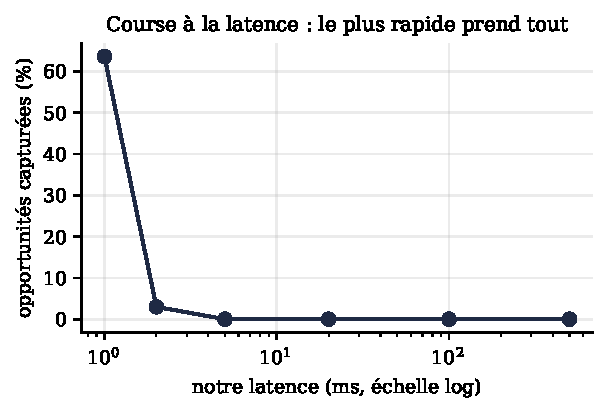
\includegraphics[width=0.6\textwidth]{ch13/course_latence.pdf}
\caption{Part des opportunités capturées en fonction de notre latence, face à des concurrents colocalisés.}
\label{c13:fig:latency}
\end{figure}

\begin{intuition}
C'est un concours où un billet tombe du ciel et où le premier qui le touche le garde. Arriver deuxième ne rapporte rien, même à un millième de seconde près. Un particulier ne gagnera jamais cette course ; il doit chercher des écarts qui ne sont pas des courses : ceux qui durent des minutes ou des jours parce qu'une friction les protège, ou ceux qui ne sont pas des arbitrages purs mais des paris de convergence (chapitre~14).
\end{intuition}

% =====================================================================
\section{Arbitrage triangulaire}
% =====================================================================

\subsection{La condition}

Trois devises EUR, USD, JPY et trois paires cotées : EUR/USD ($x$ dollars pour un euro), USD/JPY ($y$ yens pour un dollar), EUR/JPY ($z$ yens pour un euro). La cohérence impose $z = xy$. Partons d'un dollar : on achète des euros ($1/x^{ask}$ euros), avec ces euros on achète des yens ($z^{bid}/x^{ask}$ yens), avec ces yens on rachète des dollars ($z^{bid}/(x^{ask}y^{ask})$ dollars). Avec des frais $f$ à chaque étape, le cycle est profitable si
\[
\frac{z^{bid}}{x^{ask}\,y^{ask}}(1-f)^3 > 1.
\]
En points de base, si les prix milieux sont cohérents à un bruit près, le gain du cycle vaut approximativement la somme des incohérences moins trois demi-fourchettes et trois frais.

\begin{proposition}\label{c13:prop:tri}
Si l'incohérence de chacune des trois cotations est une variable normale indépendante d'écart-type $\sigma_n$ (en pb), et si chaque étape coûte une demi-fourchette $h$ et des frais $f$ (en pb), la probabilité qu'un des deux cycles soit profitable à un instant donné vaut $2\,\Prob\big(Z > \frac{3(h+f)}{\sigma_n\sqrt3}\big)$, avec $Z\sim\N(0,1)$.
\end{proposition}
\begin{proof}
Le gain du cycle direct vaut $\varepsilon_1+\varepsilon_2+\varepsilon_3 - 3(h+f)$ ; la somme des trois incohérences est normale d'écart-type $\sigma_n\sqrt3$. Le cycle inverse a pour gain l'opposé de la somme moins les mêmes coûts. Les deux événements sont disjoints (si $3(h+f)>0$) et symétriques, d'où le facteur 2.
\end{proof}

\begin{codebox}[ — E2, fréquence des opportunités triangulaires]
\textbf{Protocole :} un million d'instantanés de trois cotations. \textbf{Résultats :} demi-fourchette de 0,5 pb sans frais : $0{,}002\,\%$ des instantanés si les cotations sont cohérentes à 0,2 pb près, $38{,}6\,\%$ si elles ne le sont qu'à 1 pb près. Avec 0,5 pb de frais : 0 et $8{,}4\,\%$. Avec 2 pb de frais, niveau typique d'un particulier : $0$ et $0{,}002\,\%$. La formule de la proposition~\ref{c13:prop:tri} reproduit ces fréquences. Quand une opportunité existe, le gain moyen est inférieur à 1 pb.
\end{codebox}

Sur le marché des changes, les teneurs de marché maintiennent la cohérence des cotations croisées à une fraction de la fourchette ; les rares incohérences durent quelques millisecondes et reviennent aux plus rapides, avec des frais quasi nuls. Pour un particulier, l'arbitrage triangulaire sur le marché des changes ou sur les principales cryptomonnaies est un mirage.

% =====================================================================
\section{L'arbitrage de latence : une ligne rouge}
% =====================================================================

Une variante très répandue chez les particuliers consiste à exploiter le retard du flux de prix d'un courtier de CFD ou d'une \emph{prop firm} par rapport à un flux plus rapide : quand le prix \og vrai\fg{} bouge, on achète chez le courtier au prix encore ancien. Ce n'est pas un arbitrage entre deux marchés, c'est l'exploitation d'une faiblesse technique du fournisseur, qui en supporte directement la perte. Les conditions générales des courtiers et des \emph{prop firms} l'interdisent explicitement ; elles interdisent aussi la couverture croisée entre comptes \citep{nexusfi}. Les conséquences vont de l'annulation des gains à la fermeture du compte. Ce cours ne traite pas de ces pratiques, sauf pour vous dire de ne pas les déployer, en particulier sur vos comptes de \emph{prop firms}.

% =====================================================================
\section{Ce que la théorie apporte, et ses limites}
% =====================================================================

\paragraph{Apports.} Des conditions exactes avec frais, une explication de la persistance de certains écarts (frictions), un modèle simple de la course à la latence, et un critère d'inventaire pour l'arbitrage entre plateformes.

\paragraph{Limites.} Les opportunités réelles dépendent de la profondeur du carnet (on ne peut souvent exécuter qu'une petite quantité au meilleur prix), du risque de contrepartie des plateformes, des délais et des coûts de transfert, et de contraintes réglementaires et fiscales que les modèles ignorent.

% =====================================================================
\section{Fiche à recopier au tableau blanc}
% =====================================================================

\begin{whiteboard}
\begin{itemize}[leftmargin=1.2em]
\item \textbf{Spatial :} opportunité si $b_B/a_A > (1+f_A)/(1-f_B)\approx1+f_A+f_B$.
\item \textbf{Inventaire :} rééquilibrage rentable si $Q > 10^4K/e$ ($K$ coût de transfert, $e$ avantage en pb).
\item \textbf{Écart persistant :} chercher la friction (contrôle des capitaux, transfert, contrepartie).
\item \textbf{Latence :} le premier prend tout ; durée de vie en millisecondes $\Rightarrow$ inaccessible au particulier.
\item \textbf{Triangulaire :} profitable si $z^{bid}(1-f)^3/(x^{ask}y^{ask}) > 1$ ; probabilité $2\Prob(Z > 3(h+f)/(\sigma_n\sqrt3))$.
\item \textbf{Ligne rouge :} arbitrage de latence contre un courtier ou une \emph{prop firm} : interdit.
\end{itemize}
\end{whiteboard}

% =====================================================================
\section{Exercices}
% =====================================================================

\begin{exercise}
Le BTC est coté $64\,000$ à la vente sur A et $64\,050$ à l'achat sur B ; frais taker de 0,10\,\% sur A et 0,06\,\% sur B. Y a-t-il une opportunité ? Quel écart minimal faudrait-il ?
\end{exercise}

\begin{exercise}
Démontrez l'approximation $(1+f_A)/(1-f_B)\approx 1+f_A+f_B$ par un développement limité à l'ordre 1, et estimez l'erreur pour $f_A = f_B = 0{,}1\,\%$.
\end{exercise}

\begin{exercise}
Un inventaire de $20\,000$\,\$ par côté, un avantage moyen de 4 pb par arbitrage de $1\,000$\,\$, un coût de rééquilibrage de 15\,\$. Le rééquilibrage est-il rentable ? Combien d'arbitrages faut-il entre deux rééquilibrages ?
\end{exercise}

\begin{exercise}[à coder]
Dans E1, donnez aux opportunités une durée de vie qui dépend de leur taille (les grands écarts disparaissent plus vite). Comment évolue le gain moyen d'un acteur lent ?
\end{exercise}

% =====================================================================
\section{Pour aller plus loin}
% =====================================================================

\begin{toread}
\begin{itemize}[leftmargin=1.2em]
\item \citet{makarov2020} : les sections sur les écarts entre pays et sur le rôle des contrôles de capitaux.
\item \citet{budish2015} : la section empirique sur la durée des opportunités ES/SPY et l'argument de la course aux armements.
\item \citet{harris2003} : les chapitres consacrés aux arbitragistes et à la fragmentation des marchés.
\end{itemize}
\end{toread}

\section{Scripts du chapitre}
\noindent\texttt{code/ch13/ch13\_spatial\_triangular.py} : E1 (figure~\ref{c13:fig:latency}), E2.

% =====================================================================
\chapter{Arbitrage de base, \emph{cash-and-carry} et \emph{funding}}
\label{ch:14}
% =====================================================================

\section{Objectifs et organisation du chapitre}

\paragraph{Objectifs.} Le chapitre~13 a montré que l'arbitrage pur entre plateformes est une course perdue d'avance pour un particulier. Les quasi-arbitrages de convergence, eux, reposent sur une ancre contractuelle et se jouent sur des jours ou des semaines. À la fin du chapitre, vous saurez : (1) dériver le prix d'un contrat à terme par absence d'arbitrage et sa bande en présence de frictions ; (2) décrire le mécanisme de \emph{funding} des contrats perpétuels ; (3) évaluer un portage \emph{cash-and-carry} et son risque de chemin ; (4) choisir un levier en tenant compte du risque de liquidation ; (5) comprendre la logique des stratégies d'\texttt{atjte} entre une plateforme crypto et un CFD sur MetaTrader~5.

\paragraph{Code.} \texttt{code/ch14/ch14\_basis\_funding.py}.

% =====================================================================
\section{Le prix d'un contrat à terme}
% =====================================================================

\subsection{La relation de portage}

Un contrat à terme d'échéance $T$ engage à acheter le sous-jacent au prix $F$ convenu aujourd'hui. Soit $S$ le prix comptant, $r$ le taux d'intérêt (composé continûment), $q$ le rendement versé par le sous-jacent (dividendes, ou coût de stockage compté négativement).

\begin{proposition}[Portage]\label{c14:prop:carry}
En l'absence d'arbitrage et de frictions, $F = S\,e^{(r-q)T}$.
\end{proposition}
\begin{proof}
\emph{Si $F > Se^{(r-q)T}$} : on emprunte $Se^{-qT}$, on achète le sous-jacent (en réinvestissant ses revenus, on détient $e^{qT}$ unités à l'échéance ; on en achète donc $e^{-qT}$ au départ, pour $Se^{-qT}$) et on vend le contrat. À l'échéance, on livre le sous-jacent contre $F$ et on rembourse $Se^{-qT}e^{rT}$. Gain certain : $F - Se^{(r-q)T} > 0$, sans mise de fonds. \emph{Si $F < Se^{(r-q)T}$} : opérations inverses (vente à découvert du sous-jacent, prêt du produit, achat du contrat), gain certain $Se^{(r-q)T} - F > 0$. Les deux cas sont des arbitrages au sens de la définition~\ref{c1:def:arb} ; l'égalité est la seule possibilité.
\end{proof}

La \emph{base} est l'écart $F - S$ ; elle \og fond\fg{} jusqu'à zéro à l'échéance. Avec $r = 4\,\%$ et $q = 0$, un contrat à trois mois se traite environ $1\,\%$ au-dessus du comptant.

\subsection{Bande de non-arbitrage}

Avec des frictions (taux d'emprunt $r_b$ supérieur au taux de prêt $r_l$, coût d'emprunt du sous-jacent, frais de transaction $c$ sur chaque opération), chaque sens de l'arbitrage a son propre seuil :
\[
S\,e^{(r_l - q)T} - c' \;\le\; F \;\le\; S\,e^{(r_b - q)T} + c,
\]
où $c'$ inclut le coût d'emprunt du sous-jacent. Entre ces bornes, $F$ peut flotter sans arbitrage possible \citep{hull2022}.

\begin{intuition}
Le prix à terme est le prix comptant \og transporté dans le temps\fg{} : il faut payer le loyer de l'argent immobilisé (les intérêts) et l'on encaisse les revenus de l'actif. Si quelqu'un vous propose de livrer dans trois mois à un prix supérieur au comptant plus le loyer, vous achetez aujourd'hui, vous stockez et vous livrez : c'est le \emph{cash-and-carry}.
\end{intuition}

\subsection{Gain certain, chemin incertain}

\begin{codebox}[ — E1, cash-and-carry sur un future à 3 mois]
\textbf{Protocole :} comptant à 100, volatilité 20\,\%, taux 4\,\%, future coté $1\,\%$ au-dessus de son prix théorique, écart qui converge vers 0 à l'échéance (pont brownien) ; position longue comptant financée, courte future ; 20\,000 trajectoires. \textbf{Résultats} (pour 100 de notionnel) : gain final $1{,}01$ dans tous les cas (écart-type nul), égal à la théorie. Mais pire perte latente médiane $-0{,}13$, quantile 1\,\% $-0{,}82$ ; appel de marge cumulé maximal sur le future : médiane $5{,}0$, quantile 99\,\% $26{,}3$.
\end{codebox}

\begin{figure}[h]
\centering
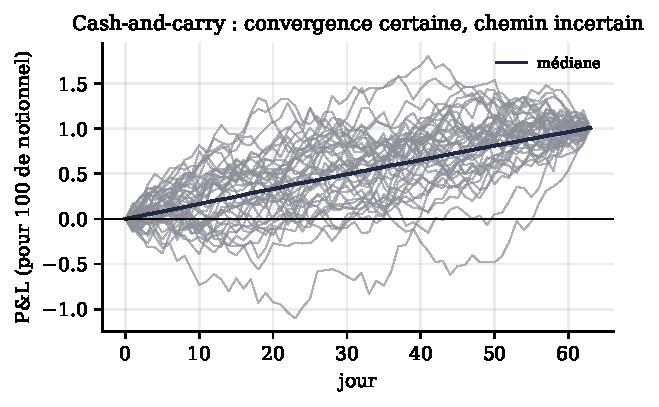
\includegraphics[width=0.62\textwidth]{ch14/cash_and_carry.pdf}
\caption{P\&L de 40 trajectoires d'un \emph{cash-and-carry} : toutes finissent au même gain, après des chemins différents.}
\label{c14:fig:cc}
\end{figure}

\paragraph{Lecture.} Le gain final est connu, mais si le comptant monte de 25\,\%, la jambe courte du future réclame 25 de marge \emph{en espèces}, alors que le gain de la jambe comptant est latent (sauf si l'on peut l'emprunter). Le risque d'un \emph{cash-and-carry} n'est pas le résultat final, c'est la liquidité nécessaire pour tenir jusqu'au bout. C'est exactement le mécanisme des limites de l'arbitrage de \citet{shleifer1997}.

% =====================================================================
\section{Les contrats perpétuels}
% =====================================================================

\subsection{Le mécanisme de \emph{funding}}

Un contrat perpétuel est un contrat à terme sans échéance, très répandu sur les plateformes de cryptomonnaies. Rien ne force sa convergence vers le comptant ; à la place, un paiement périodique (le \emph{funding}, souvent toutes les 8 heures, parfois toutes les heures) circule entre acheteurs et vendeurs. Quand le perpétuel cote au-dessus de l'indice comptant, le taux est positif et les positions longues paient les courtes ; quand il cote en dessous, l'inverse. Le taux combine en général une composante de prime (écart entre le perpétuel et l'indice) et une composante d'intérêt, avec des bornes ; \emph{la formule exacte dépend de chaque plateforme} et doit être lue dans sa documentation.

\citet{he2022perp} dérivent les prix d'absence d'arbitrage des perpétuels sans frictions et des bornes avec coûts de transaction ; ils trouvent que les écarts aux prix théoriques sont plus importants en crypto que sur les marchés de change traditionnels, qu'ils évoluent ensemble d'une cryptomonnaie à l'autre et qu'ils se réduisent avec le temps, et qu'une stratégie d'arbitrage fondée sur ces écarts aurait obtenu des ratios de Sharpe élevés.

\subsection{Le portage du \emph{funding}}

La stratégie la plus simple : acheter le comptant et vendre le perpétuel en même quantité. La position est neutre au prix ; elle encaisse le \emph{funding} tant qu'il est positif. Les risques :
\begin{enumerate}
\item le \emph{funding} peut devenir négatif pendant des périodes prolongées ;
\item la jambe courte est sur marge : une forte hausse peut la liquider, laissant la jambe comptant seule, non couverte ;
\item risque de contrepartie de la plateforme qui détient les deux jambes ou l'une d'elles ;
\item écart entre le perpétuel et le comptant au moment d'entrer et de sortir.
\end{enumerate}

\paragraph{Distance de liquidation.} Avec un levier $L$ sur la jambe courte (marge initiale $1/L$ du notionnel) et une marge de maintien $m$, la position est liquidée si le prix monte d'environ $1/L - m$ sans que la marge soit réapprovisionnée.

\begin{codebox}[ — E2, portage du \emph{funding} selon le levier]
\textbf{Protocole :} 5\,000 années simulées ; volatilité 60\,\% par an plus des sauts (environ quatre par an, d'écart-type 8\,\%) ; \emph{funding} quotidien autoregressif de moyenne $\approx10\,\%$ par an, négatif un jour sur trois ; marge réapprovisionnée chaque jour ; capital engagé = comptant + marge. \textbf{Résultats :}
\begin{center}\small
\begin{tabular}{rcccc}
\toprule
Levier & hausse liquidante (1 jour) & probabilité de liquidation & rendement moyen & quantile 5\,\% \\
\midrule
1 & 99,5\,\% & 0 & 5,0\,\% & $-2{,}4\,\%$\\
2 & 49,5\,\% & 0 & 6,6\,\% & $-3{,}2\,\%$\\
3 & 32,8\,\% & 0,2\,\% & 7,5\,\% & $-3{,}6\,\%$\\
5 & 19,5\,\% & 7,4\,\% & 7,9\,\% & $-4{,}0\,\%$\\
10 & 9,5\,\% & 71,7\,\% & 4,5\,\% & $-3{,}9\,\%$\\
\bottomrule
\end{tabular}
\end{center}
\end{codebox}

\paragraph{Lecture.} Le levier améliore le rendement sur capital tant qu'il n'expose pas à la liquidation ; au-delà, le rendement s'effondre, et le modèle sous-estime encore le danger : il suppose que la marge est réapprovisionnée chaque jour et ignore les mouvements intrajournaliers, l'écart entre perpétuel et comptant au moment de la liquidation, et la possibilité que la plateforme elle-même suspende les retraits.

% =====================================================================
\section{Étude de cas : les stratégies d'\texttt{atjte}}
% =====================================================================

\subsection{Le principe}

Le moteur \texttt{atjte} \citep{atjte} (chapitre~0, section~\ref{c0:atjte}) trade un écart entre deux instruments qui portent le même sous-jacent, par exemple un perpétuel ou un jeton adossé à l'or sur une plateforme crypto et le CFD XAUUSD chez un courtier MetaTrader~5 :
\[
s_t = P^{\text{plateforme}}_t - k\,P^{\text{MT5}}_t,
\]
où $k$ convertit les unités. Les ordres sont des ordres limites \emph{maker} sur la plateforme crypto, placés à $k\,P^{\text{MT5}}_{\text{bid}} + \text{niveau}$ à l'achat (et symétriquement à la vente), si bien qu'une exécution correspond à un écart égal au niveau visé, net de la fourchette du CFD. Chaque exécution est immédiatement couverte par un ordre au marché opposé sur MT5.

\subsection{Les stratégies fournies}

\begin{itemize}
\item \textbf{Niveaux fixes} : un ordre d'achat et un ordre de vente à des niveaux d'écart fixés.
\item \textbf{Grille} : plusieurs niveaux, pour accumuler une position quand l'écart s'éloigne.
\item \textbf{Bandes de Bollinger} : niveaux placés à la moyenne glissante de l'écart $\pm$ un multiple de son écart-type (fenêtre en minutes, échantillons à la seconde).
\item \textbf{Grille sur future daté} : le centre de la grille est la base \og juste\fg{} $=$ centre $+$ prix de référence $\times$ taux de portage annuel $\times$ jours restants$/365$, recalculée une fois par jour ; plus de nouvelle entrée à l'approche de l'échéance.
\end{itemize}

\subsection{Pourquoi le centre compte}

Quand la base a une composante déterministe (portage qui fond, écart de frais comme pour GLD/GLDM au chapitre~3, ou \emph{funding} moyen), où placer le centre des niveaux ?

\begin{codebox}[ — E3, centre fixe, moyenne glissante ou base théorique]
\textbf{Protocole :} base d'un future daté à un an avec portage de 4\,\% qui fond jusqu'à l'échéance, plus un écart AR(1) de demi-vie 3 jours autour de la base théorique ; trading sur 3 ans avec roulement annuel ; seuils $\pm1{,}5$ écart-type ; 4 pb par changement de position ; le P\&L inclut le portage (intérêts reçus ou payés), qui compense exactement la fonte de la base théorique. 300 simulations. \textbf{Résultats} (gain en pb par an) : centre fixe estimé sur un an $11{,}3$ (écart-type $14{,}4$) ; bandes de Bollinger sur 20 jours $73{,}3$ ($26{,}3$) ; base théorique $217{,}0$ ($34{,}1$).
\end{codebox}

\paragraph{Lecture.} Un centre fixe confond la fonte mécanique de la base avec un écart à corriger ; une moyenne glissante la suit mais avec retard, et son écart-type glissant est bruité ; un centre théorique isole exactement la partie aléatoire de l'écart. Quand une ancre théorique existe, il faut s'en servir : c'est ce que fait la stratégie de grille sur future daté d'\texttt{atjte}.

\begin{pitfall}
Sur la jambe CFD, le courtier facture des frais de financement de nuit (\emph{swap}) qui dépendent du sens de la position et de ses propres conditions ; sur un perpétuel, c'est le \emph{funding}. Ces deux portages ne se compensent pas forcément, et leur différence est un coût (ou un gain) permanent de la stratégie qu'il faut modéliser. Enfin, les règles des \emph{prop firms} interdisent ce type de couverture entre comptes ou plateformes : ces stratégies se déploient sur capital propre, chez des courtiers qui les acceptent.
\end{pitfall}

% =====================================================================
\section{Ce que la théorie apporte, et ses limites}
% =====================================================================

\paragraph{Apports.} Une ancre de prix exacte pour les contrats datés, une bande de non-arbitrage avec frictions, une compréhension du \emph{funding} comme substitut de la convergence, et un critère de levier fondé sur la distance de liquidation.

\paragraph{Limites.} Les perpétuels n'ont pas d'ancre stricte : l'écart peut rester large longtemps. Le risque de contrepartie des plateformes est réel et non diversifiable à l'intérieur d'une même plateforme. Les règles de marge, de liquidation et de \emph{funding} changent d'une plateforme à l'autre et dans le temps. Les besoins de liquidité peuvent forcer une sortie avant la convergence.

% =====================================================================
\section{Fiche à recopier au tableau blanc}
% =====================================================================

\begin{whiteboard}
\begin{itemize}[leftmargin=1.2em]
\item \textbf{Portage :} $F = Se^{(r-q)T}$ ; base $F - S\to0$ à l'échéance.
\item \textbf{Bande :} $Se^{(r_l-q)T} - c' \le F \le Se^{(r_b-q)T} + c$.
\item \textbf{Cash-and-carry :} long comptant financé, court future ; gain final fixé, besoin de marge variable.
\item \textbf{Funding :} longs paient les courts si perpétuel $>$ indice ; formule propre à chaque plateforme.
\item \textbf{Liquidation :} hausse de $\approx 1/L - m$ sur la jambe courte.
\item \textbf{atjte :} $s_t = P^{\text{plat}} - kP^{\text{MT5}}$ ; maker sur la plateforme, taker sur MT5 ; centre théorique $=$ référence $\times$ portage $\times$ jours$/365$.
\end{itemize}
\end{whiteboard}

% =====================================================================
\section{Exercices}
% =====================================================================

\begin{exercise}
L'or comptant vaut 4\,000, le taux est de 4\,\%, le coût de stockage de 0,1\,\% par an. Quel est le prix théorique du contrat à 6 mois ? Quelle est la base en dollars et en points de base ?
\end{exercise}

\begin{exercise}
Le \emph{funding} moyen est de 0,01\,\% toutes les 8 heures. Calculez le rendement annuel brut d'un portage sans levier, puis le rendement sur capital avec un levier de 3 sur la jambe courte.
\end{exercise}

\begin{exercise}
Justifiez la formule de distance de liquidation $1/L - m$ à partir de la définition de la marge.
\end{exercise}

\begin{exercise}[à coder]
Dans E2, remplacez le réapprovisionnement quotidien de la marge par un réapprovisionnement hebdomadaire. Comment change la probabilité de liquidation pour un levier de 3 ?
\end{exercise}

\begin{exercise}[à coder]
Reprenez E3 en ajoutant un écart constant de 10 pb par an entre le \emph{swap} du CFD et le portage de la plateforme. Comment faut-il modifier le centre théorique ?
\end{exercise}

% =====================================================================
\section{Pour aller plus loin}
% =====================================================================

\begin{toread}
\begin{itemize}[leftmargin=1.2em]
\item \citet{hull2022} : les chapitres sur la détermination des prix à terme et sur les futures de matières premières.
\item \citet{he2022perp} : théorie des prix des perpétuels et mesure des écarts.
\item \citet{shleifer1997} : pourquoi un arbitrage à gain final certain peut tout de même échouer.
\item Le code d'\texttt{atjte} \citep{atjte} : \texttt{strategy\_types/arb/bollinger\_bot} et \texttt{grid\_futures\_bot}, et le module \texttt{engines/common/ratio.py} pour le contrôle du ratio $k$.
\end{itemize}
\end{toread}

\section{Scripts du chapitre}
\noindent\texttt{code/ch14/ch14\_basis\_funding.py} : E1 (figure~\ref{c14:fig:cc}), E2, E3.

% =====================================================================
\chapter{Exécution, couverture et architecture logicielle}
\label{ch:15}
% =====================================================================

\section{Objectifs et organisation du chapitre}

\paragraph{Objectifs.} Le dépôt \texttt{atjte} contient beaucoup plus de code d'exécution que de code de signal : c'est la réalité de l'arbitrage entre plateformes. À la fin du chapitre, vous saurez : (1) identifier le risque de jambe et le quantifier ; (2) expliquer la sélection adverse d'un ordre \emph{maker} couvert sur une autre plateforme ; (3) mesurer l'effet du retard de recotation et de la latence de couverture ; (4) choisir sur quelle plateforme coter ; (5) concevoir une architecture qui survive aux pannes, aux déconnexions et aux erreurs humaines.

\paragraph{Code.} \texttt{code/ch15/ch15\_execution.py}.

% =====================================================================
\section{Le risque de jambe}
% =====================================================================

Un trade de paire comporte deux ordres sur deux instruments, souvent sur deux plateformes. Ils ne sont jamais exécutés exactement au même instant ni au prix prévu. Entre les deux exécutions, le prix bouge : c'est le \emph{risque de jambe} (\emph{leg risk}). Dans le pire des cas, une jambe est exécutée et l'autre est refusée (déconnexion, marge insuffisante, marché fermé) : on se retrouve avec une position directionnelle non voulue.

\begin{proposition}\label{c15:prop:leg}
Si le prix suit une marche aléatoire de volatilité $\sigma$ par unité de temps et que les deux exécutions sont séparées d'un délai $\Delta$, l'écart réalisé diffère de l'écart visé d'une quantité d'espérance nulle et d'écart-type $\sigma\sqrt\Delta$.
\end{proposition}
\begin{proof}
C'est la proposition~\ref{c1:prop:rw} appliquée sur la durée $\Delta$ : l'accroissement d'une marche aléatoire sur $\Delta$ unités de temps a une variance $\sigma^2\Delta$.
\end{proof}

\begin{codebox}[ — E3, risque de jambe d'une exécution taker-taker (or, volatilité 15\,\% par an)]
Écart-type de l'écart réalisé : $0{,}06$ pb pour un décalage de 10 ms, $0{,}20$ pb pour 100 ms, $0{,}62$ pb pour 1 s, $1{,}38$ pb pour 5 s (conformes à $\sigma\sqrt\Delta$) ; quantile 1\,\% : $-1{,}4$ pb à 1 s et $-3{,}2$ pb à 5 s. Pour une cryptomonnaie de volatilité 60\,\%, tous ces nombres sont multipliés par 4.
\end{codebox}

Le risque de jambe est d'espérance nulle si le délai est indépendant des mouvements de prix. Il devient un coût quand il ne l'est pas, ce qui est précisément le cas des ordres \emph{maker}.

% =====================================================================
\section{La sélection adverse d'un ordre \emph{maker}}
% =====================================================================

\subsection{Le mécanisme}

Une stratégie \emph{maker-taker} (comme celle d'\texttt{atjte}) affiche un ordre limite sur la plateforme A à un prix calculé à partir de la plateforme de référence B, attend d'être exécutée, puis couvre immédiatement sur B au marché. Le prix affiché doit être recalculé à chaque mouvement de B. Si la recotation a du retard, l'ordre affiché devient \og périmé\fg{} : quand B baisse, notre prix d'achat sur A reste trop haut un instant, et c'est précisément à ce moment que quelqu'un vient nous vendre. On est exécuté quand on a tort.

\begin{intuition}
Vous affichez dans votre vitrine un prix d'achat pour de l'or, calculé d'après le cours de ce matin. Si le cours chute à midi et que vous ne changez pas l'étiquette, tous les vendeurs du quartier viennent chez vous. Vous ferez beaucoup d'affaires, toutes mauvaises.
\end{intuition}

\subsection{Expérience}

\begin{codebox}[ — E1 et E2, glissement d'un achat maker couvert]
\textbf{Protocole :} prix de l'or simulé au pas de 50 ms pendant 4 heures ; la plateforme A suit B avec 200 ms de retard (E1) ou la précède de 200 ms (E2), avec un bruit de base ; ordre d'achat maker sur A à $1{,}2$\,\$ sous le prix acheteur de B ; couverture par une vente au prix acheteur de B. Le glissement mesure l'écart réalisé moins l'écart visé (négatif : perte). Environ 1\,900 exécutions par configuration. \textbf{Résultats} (glissement moyen, pb) :
\begin{center}\small
\begin{tabular}{lcccccc}
\toprule
 & \multicolumn{3}{c}{A suit B} & \multicolumn{3}{c}{A précède B}\\
\cmidrule(lr){2-4}\cmidrule(lr){5-7}
Retard de recotation & couv. 50 ms & 500 ms & 2 s & 50 ms & 500 ms & 2 s\\
\midrule
0 ms & $0{,}00$ & $0{,}00$ & $+0{,}02$ & $-0{,}01$ & $-0{,}13$ & $-0{,}11$\\
100 ms & $0{,}00$ & $0{,}00$ & $+0{,}01$ & $-0{,}02$ & $-0{,}13$ & $-0{,}13$\\
500 ms & $-0{,}15$ & $-0{,}16$ & $-0{,}14$ & $-0{,}09$ & $-0{,}21$ & $-0{,}20$\\
2 s & $-0{,}47$ & $-0{,}48$ & $-0{,}50$ & $-0{,}38$ & $-0{,}51$ & $-0{,}51$\\
\bottomrule
\end{tabular}
\end{center}
\end{codebox}

\begin{figure}[h]
\centering
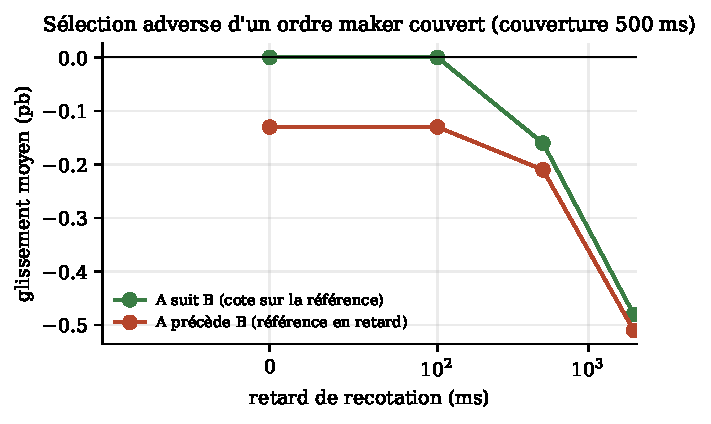
\includegraphics[width=0.66\textwidth]{ch15/selection_adverse.pdf}
\caption{Glissement moyen d'un achat maker couvert en fonction du retard de recotation, selon que la plateforme où l'on cote suit ou précède la référence.}
\label{c15:fig:adverse}
\end{figure}

\paragraph{Lecture.} (1) Tant que l'on recote vite et que l'on cote sur la plateforme \emph{suiveuse} (A suit B), le glissement est nul : notre prix bouge avant que le marché de A ne vienne le chercher. (2) Un retard de recotation de 2 s coûte environ $0{,}5$ pb par exécution, soit près d'un sixième d'un avantage visé de 3 pb. (3) Si l'on cote sur la plateforme \emph{meneuse} (A précède B), on est en retard par construction : même avec une recotation instantanée, la couverture sur B arrive après le mouvement. (4) Ces chiffres sont calculés pour l'or ; ils sont proportionnels à la volatilité et à la racine du retard, donc environ quatre fois plus grands pour une cryptomonnaie. Mesurer la relation meneur-suiveur entre ses deux plateformes (corrélation des variations décalées) est un préalable à toute stratégie maker-taker.

% =====================================================================
\section{Architecture : leçons d'\texttt{atjte}}
% =====================================================================

Le dépôt \texttt{atjte} \citep{atjte} illustre les choix d'architecture qu'impose une stratégie réelle. Les éléments suivants sont décrits dans sa documentation et son code.

\begin{description}
\item[Passerelles (\emph{gateways}).] Chaque plateforme est atteinte par un processus séparé qui détient seul les clés et les connexions ; les robots ne voient jamais de clé et passent par la passerelle en local. Une erreur dans un robot ne peut pas fuiter une clé ni ouvrir une connexion non contrôlée.
\item[Contrôle du ratio.] Le ratio $k$ (unités MT5 par unité de la plateforme) est vérifié au démarrage et en continu contre le rapport des prix, avec une tolérance de $\pm10\,\%$ : une erreur d'unité (facteur 10, inversion, onces contre grammes) est bloquée avant de couvrir dix fois trop ou trop peu.
\item[Seuils de couverture et lot minimal.] Une exposition inférieure au lot minimal du courtier ne peut pas être couverte ; le code avertit quand le seuil de couverture représente plus de deux lots minimaux, cas où une exposition significative resterait non couverte.
\item[Réconciliation.] La couverture et les contrôles portent sur l'exposition réelle relue sur les deux plateformes, pas sur le registre interne du robot ; un écart est vérifié une seconde fois avant correction, pour ne pas réagir à un état transitoire.
\item[Flux temps réel obligatoires.] Si le flux de prix est périmé ou si le flux des exécutions n'est pas confirmé, le robot annule ses ordres et se met en sommeil plutôt que de coter sur des données anciennes.
\item[Un robot par contrat.] Toutes les stratégies d'un même contrat partagent la position et le livre de couverture ; le démarrage est refusé si un autre robot est actif sur le même contrat.
\item[Mode simulation.] Rien n'est envoyé tant que \texttt{LIVE\_TRADING} n'est pas explicitement activé.
\item[Journalisation.] L'état du compte, les exécutions et l'historique de l'écart sont écrits en continu sur disque, pour reconstruire après coup ce qui s'est passé.
\end{description}

\begin{pitfall}
Chacun de ces mécanismes répond à un incident possible : couverture dans la mauvaise unité, exposition résiduelle sous le lot minimal, double robot sur le même compte, ordre envoyé sur une donnée vieille de dix secondes, plateforme qui ne confirme pas une exécution. Le dépôt rappelle lui-même qu'il a été écrit en grande partie avec des assistants de programmation et n'a pas été audité. Avant de confier de l'argent à un code, quel qu'il soit, lisez-le, testez-le en simulation, puis avec de petites tailles.
\end{pitfall}

\subsection{Liste de contrôle d'un moteur d'exécution}

\begin{enumerate}
\item Identifiants d'ordre uniques côté client, pour qu'un ordre renvoyé après une coupure ne soit pas exécuté deux fois.
\item Limitation du débit des requêtes (seau à jetons) pour respecter les quotas des plateformes.
\item Annulation automatique des ordres si le robot cesse de donner signe de vie (\emph{dead man's switch}), côté plateforme quand elle le propose.
\item Limites de risque indépendantes du signal : position maximale, perte journalière maximale, exposition non couverte maximale, plages horaires interdites (annonces, ouverture et maintenance des marchés).
\item Persistance de l'état et reprise propre après redémarrage.
\item Surveillance et alertes (téléphone) en cas d'écart de réconciliation, de rejet d'ordre ou de flux muet.
\end{enumerate}

% =====================================================================
\section{Ce que la théorie apporte, et ses limites}
% =====================================================================

\paragraph{Apports.} Une quantification du risque de jambe ($\sigma\sqrt\Delta$), une compréhension mécanique de la sélection adverse, et un critère pour choisir où coter (sur la plateforme suiveuse, avec une recotation rapide).

\paragraph{Limites.} Le modèle ignore la file d'attente (on n'est pas forcément servi au premier passage du prix), les exécutions partielles, les rejets, les pannes et la profondeur des carnets. Seuls des journaux d'exécution réels permettent de mesurer la sélection adverse effective.

% =====================================================================
\section{Fiche à recopier au tableau blanc}
% =====================================================================

\begin{whiteboard}
\begin{itemize}[leftmargin=1.2em]
\item \textbf{Risque de jambe :} écart-type $\sigma\sqrt\Delta$ ; nul en espérance seulement si le délai est indépendant des prix.
\item \textbf{Sélection adverse :} un ordre maker est exécuté quand le marché lui donne tort ; coût croissant avec le retard de recotation.
\item \textbf{Où coter :} sur la plateforme suiveuse ; couvrir sur la meneuse.
\item \textbf{Architecture :} passerelles, contrôle du ratio, lot minimal, réconciliation sur positions réelles, sommeil si flux périmé, un robot par contrat, mode simulation, journaux.
\end{itemize}
\end{whiteboard}

% =====================================================================
\section{Exercices}
% =====================================================================

\begin{exercise}
Une cryptomonnaie a une volatilité annuelle de 70\,\% (365 jours de 24 h). Calculez l'écart-type du risque de jambe pour un décalage de 300 ms.
\end{exercise}

\begin{exercise}
Pourquoi le glissement de E1 est-il légèrement positif pour une couverture à 2 s quand A suit B ? (Indice : que fait le bruit de base de A entre l'exécution et la couverture ?)
\end{exercise}

\begin{exercise}[à coder]
Ajoutez à E1 une file d'attente : on n'est exécuté que si le prix de A passe au moins 0,1\,\$ sous notre prix. Comment changent le nombre d'exécutions et le glissement ?
\end{exercise}

\begin{exercise}[données réelles]
Enregistrez pendant une journée les prix milieux de l'or sur deux plateformes au pas de la seconde. Calculez la corrélation entre les variations de l'une et les variations décalées de l'autre pour des décalages de $-5$ à $+5$ s. Laquelle mène ?
\end{exercise}

% =====================================================================
\section{Pour aller plus loin}
% =====================================================================

\begin{toread}
\begin{itemize}[leftmargin=1.2em]
\item \citet{harris2003} : les chapitres sur les fournisseurs de liquidité et la sélection adverse.
\item \citet{budish2015} : pourquoi les cotations périmées sont \og attrapées\fg{} par les plus rapides.
\item Le code d'\texttt{atjte} \citep{atjte} : \texttt{engines/arb/arb\_bot.py} (boucle principale, couverture, réconciliation), \texttt{engines/common/hedge\_gate.py} et \texttt{ratio.py}, \texttt{gateways/}.
\end{itemize}
\end{toread}

\section{Scripts du chapitre}
\noindent\texttt{code/ch15/ch15\_execution.py} : E1–E2 (figure~\ref{c15:fig:adverse}), E3.


\part{Validation, risque et mise en production}
% =====================================================================
\chapter{\emph{Backtest} rigoureux}
\label{ch:16}
% =====================================================================

\section{Objectifs et organisation du chapitre}

\paragraph{Objectifs.} Un \emph{backtest} rejoue une stratégie sur des données passées pour estimer ce qu'elle aurait rapporté. C'est l'outil central du trader quantitatif, et c'est aussi le meilleur moyen de se mentir. À la fin du chapitre, vous saurez : (1) reconnaître et éliminer les biais d'anticipation, de survie et de sélection ; (2) organiser formation, validation et test sans fuite d'information ; (3) calculer l'erreur-type d'un ratio de Sharpe et savoir combien d'années il faut pour distinguer un bon Sharpe du hasard ; (4) corriger un Sharpe du nombre de variantes essayées (ratio de Sharpe déflaté) ; (5) estimer la probabilité qu'une optimisation soit du surapprentissage (PBO) ; (6) utiliser le moteur de \emph{backtest} du paquet \texttt{arbhub}, testé contre l'anticipation.

\paragraph{Code.} \texttt{code/ch16/ch16\_backtest.py} (expériences E1 à E6), et les modules réutilisables \texttt{src/arbhub/backtest/engine.py} et \texttt{metrics.py}, avec leurs tests dans \texttt{tests/test\_backtest.py}.

\begin{intuition}
Un \emph{backtest}, c'est un examen blanc dont vous auriez écrit vous-même le sujet. Si vous avez vu les réponses en écrivant le sujet (anticipation), si vous n'avez gardé que les copies des élèves qui ont réussi l'année (survie), ou si vous avez passé l'examen cinquante fois en ne retenant que la meilleure note (sélection), la note ne dit rien de ce qui se passera le jour du vrai examen. Tout ce chapitre consiste à rendre l'examen blanc aussi honnête que le vrai.
\end{intuition}

% =====================================================================
\section{Les trois biais fatals}
% =====================================================================

\subsection{Le biais d'anticipation}

\begin{definition}
Un \emph{backtest} souffre d'un \emph{biais d'anticipation} (\emph{look-ahead bias}) si une décision datée de $t$ utilise, même indirectement, une information qui n'était pas disponible à la date $t$.
\end{definition}

Les formes les plus fréquentes en arbitrage statistique sont :
\begin{enumerate}
\item \textbf{la position appliquée trop tôt :} la position décidée avec le prix de clôture de $t$ est appliquée à la variation de $t-1$ à $t$, alors qu'on ne pouvait la prendre qu'\emph{à} la clôture de $t$ ;
\item \textbf{la normalisation globale :} le \emph{z-score} est calculé avec la moyenne et l'écart-type de \emph{toute} la période ; à la date $t$, on \og sait\fg{} donc déjà autour de quel niveau l'écart finira ;
\item \textbf{le ratio de couverture global :} $\beta$ est estimé par régression sur toute la période, puis utilisé dès le premier jour ;
\item \textbf{les données révisées ou ajustées :} prix ajustés des dividendes ou des divisions calculés après coup, compositions d'indices connues après coup, données macroéconomiques révisées.
\end{enumerate}

La règle qui élimine les trois premières est celle du chapitre~1, écrite une fois pour toutes dans le moteur :
\begin{equation}\label{c16:eq:pnl}
\text{gain}_{t+1} = q_t\,(S_{t+1} - S_t), \qquad q_t = f\big(\text{données datées} \le t\big),
\end{equation}
et tous les paramètres ($\beta$, moyenne, écart-type, seuils) sont estimés soit sur une période de formation \emph{antérieure}, soit en fenêtre glissante \emph{strictement passée}.

\begin{codebox}[ — E1, un écart sans avantage rejoué de quatre façons]
\textbf{Protocole :} 300 mondes de 1\,000 jours où l'écart $y - 1{,}5x$ est une \emph{marche aléatoire} : aucune stratégie de retour à la moyenne ne peut y gagner en espérance. Règle $|z|>2$, sortie à $z=0$, \emph{z-score} glissant sur 60 jours, sans coûts. \textbf{Sharpe annualisé médian (part des mondes gagnants) :}
\begin{center}\small
\begin{tabular}{lcc}
\toprule
Implémentation & Sharpe médian & Mondes gagnants \\
\midrule
Correcte (équation~\ref{c16:eq:pnl}) & $0{,}07$ & 54,7\,\% \\
$\beta$ estimé sur toute la période & $0{,}24$ & 66,7\,\% \\
Moyenne et écart-type de toute la période & $0{,}85$ & 77,7\,\% \\
Position appliquée le jour même & $-0{,}89$ & 0,7\,\% \\
\bottomrule
\end{tabular}
\end{center}
Dans un monde \emph{avec} avantage ($\varphi = 0{,}97$), l'implémentation correcte donne un Sharpe médian de $1{,}09$ et la position appliquée le jour même $-0{,}13$.
\end{codebox}

\begin{figure}[h]
\centering
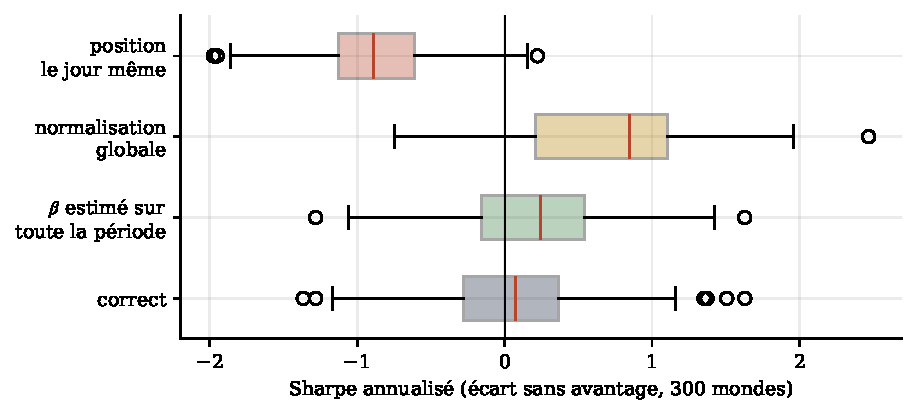
\includegraphics[width=0.72\textwidth]{ch16/biais_anticipation.pdf}
\caption{Distribution du Sharpe annualisé sur 300 mondes sans avantage, selon l'implémentation. Seule la version correcte est centrée sur zéro.}
\label{c16:fig:lookahead}
\end{figure}

\paragraph{Lecture.} La normalisation globale fabrique un Sharpe de $0{,}85$ à partir de rien : en connaissant le niveau moyen final de l'écart, on sait dans quel sens il finira par \og revenir\fg. Le $\beta$ global fait la même chose plus discrètement. L'erreur de date donne un résultat très \emph{négatif} : pour une stratégie contrariante, la position décidée en voyant un écart monter est une vente, et l'appliquer à la hausse qui vient d'avoir lieu fait perdre. Le biais d'anticipation n'a donc pas de signe fixe ; il rend simplement le résultat faux. Un \emph{backtest} anormalement mauvais mérite la même méfiance qu'un \emph{backtest} anormalement bon.

\begin{pitfall}
Le test le plus efficace contre l'anticipation n'est pas la relecture du code, c'est un test automatique : on modifie toutes les données \emph{après} une date $t_0$ et l'on vérifie que les positions et le P\&L jusqu'à $t_0$ sont inchangés. C'est le test \texttt{test\_no\_lookahead\_signal\_and\_pnl} du dépôt ; le fichier \texttt{CLAUDE.md} en exige un pour chaque nouvelle stratégie.
\end{pitfall}

\subsection{Le biais de survie}

\begin{definition}
Il y a \emph{biais de survie} quand l'univers testé ne contient que les actifs qui existent encore aujourd'hui, en excluant ceux qui ont été radiés (faillite, rachat, fusion) pendant la période.
\end{definition}

En \emph{pairs trading}, c'est particulièrement grave : une paire se rompt souvent \emph{parce que} l'une des deux sociétés subit un événement qui finit par sa radiation. Exclure les radiées revient à exclure précisément les paires qui ont perdu.

\begin{codebox}[ — E6, biais de survie]
\textbf{Protocole :} 400 paires ; 30\,\% d'entre elles subissent une rupture (l'écart se met à dériver durablement) et l'action concernée est radiée 100 jours plus tard ; règle $|z|>2$ calibrée sur 500 jours, coûts 5 pb par jambe. \textbf{Résultats :} 303 paires survivent. Sur toutes les paires, gain moyen $52{,}05$ et Sharpe médian $1{,}92$ ; sur les seules survivantes, gain moyen $62{,}86$ (+21\,\%) et Sharpe médian $2{,}03$.
\end{codebox}

La correction consiste à utiliser une base de données qui conserve les titres radiés avec leur dernier prix, et à reconstituer l'univers \emph{tel qu'il était connu à chaque date} (\emph{point-in-time}).

\subsection{Le biais de sélection et les tests multiples}

\begin{intuition}
Lancez 1\,000 pièces de monnaie dix fois chacune. Une dizaine d'entre elles feront au moins neuf \og pile\fg{} sur dix. Ce ne sont pas des pièces truquées : c'est ce qui arrive quand on regarde 1\,000 pièces. Essayer 1\,000 paires, 50 seuils ou 20 fenêtres et retenir la meilleure combinaison, c'est exactement la même chose.
\end{intuition}

Le reste du chapitre quantifie ce biais. Il faut d'abord savoir à quel point un ratio de Sharpe est imprécis, même sans sélection.

% =====================================================================
\section{L'erreur d'estimation du ratio de Sharpe}
% =====================================================================

\subsection{Définition}

Pour des rendements (ou gains) par période $r_1,\dots,r_T$, le ratio de Sharpe par période est $\widehat{SR} = \bar r/\hat s$, où $\bar r$ est la moyenne et $\hat s$ l'écart-type. Le Sharpe annualisé vaut $\widehat{SR}\sqrt{P}$, avec $P$ le nombre de périodes par an (252 en données quotidiennes). Pour une stratégie de paires, on calcule le Sharpe des gains nets rapportés au capital engagé, ou directement des gains en devise : le ratio est le même à un facteur d'échelle près.

\subsection{Erreur-type}

\begin{proposition}[\citet{lo2002}]\label{c16:prop:sese}
Si les rendements sont i.i.d. de loi normale, l'estimateur $\widehat{SR}$ est asymptotiquement normal, d'espérance $SR$ et d'écart-type
\[
\operatorname{se}(\widehat{SR}) \approx \sqrt{\frac{1 + \frac12 SR^2}{T}}.
\]
Pour des rendements i.i.d. non normaux d'asymétrie $\gamma_3$ et de kurtosis $\gamma_4$ (égale à 3 pour la loi normale), la formule devient $\sqrt{\big(1 - \gamma_3 SR + \frac{\gamma_4-1}{4}SR^2\big)/T}$ \citep{bailey2014dsr}.
\end{proposition}
\begin{proof}[Idée de la démonstration]
$\widehat{SR}$ est une fonction $g(\bar r, \hat s^2) = \bar r/\sqrt{\hat s^2}$ des deux premiers moments empiriques. Pour une loi normale, $\bar r$ et $\hat s^2$ sont indépendants, de variances $s^2/T$ et $2s^4/T$. La méthode delta donne $\Var(\widehat{SR}) \approx (\partial_1 g)^2\,s^2/T + (\partial_2 g)^2\,2s^4/T$, avec $\partial_1 g = 1/s$ et $\partial_2 g = -\bar r/(2s^3)$. D'où $\Var(\widehat{SR}) \approx 1/T + (\bar r^2/(4s^6))\,2s^4/T = (1 + SR^2/2)/T$.
\end{proof}

\paragraph{Conséquence pratique.} Le terme $SR^2/2$ est négligeable en données quotidiennes (un Sharpe annuel de 1 correspond à $SR = 1/\sqrt{252} \approx 0{,}063$ par jour). L'erreur-type du Sharpe \emph{annualisé} vaut donc environ $\sqrt{252/T} = 1/\sqrt{\text{nombre d'années}}$.

\begin{codebox}[ — E2, dispersion du Sharpe estimé d'une stratégie de vrai Sharpe annuel 1]
\textbf{Protocole :} 4\,000 simulations par durée, rendements normaux puis de Student à 4 degrés de liberté (queues épaisses). \textbf{Écart-type du Sharpe annualisé estimé :}
\begin{center}\small
\begin{tabular}{rcccc}
\toprule
Durée & Normal & Formule de Lo & Student(4) & Intervalle à 95\,\% (normal) \\
\midrule
1 an & 0,981 & 1,003 & 1,012 & $[-0{,}92\,;\,2{,}92]$ \\
3 ans & 0,581 & 0,578 & 0,580 & $[-0{,}14\,;\,2{,}14]$ \\
5 ans & 0,442 & 0,448 & 0,447 & $[0{,}13\,;\,1{,}87]$ \\
10 ans & 0,316 & 0,317 & 0,316 & $[0{,}38\,;\,1{,}62]$ \\
\bottomrule
\end{tabular}
\end{center}
\end{codebox}

\paragraph{Lecture.} Avec un an de données, une stratégie de vrai Sharpe 1 affiche un Sharpe estimé n'importe où entre $-0{,}9$ et $2{,}9$. Il faut environ cinq ans pour que l'intervalle à 95\,\% exclue zéro. En données quotidiennes, les queues épaisses changent très peu l'erreur-type (le terme en $\gamma_4$ est multiplié par $SR^2$, minuscule) ; elles comptent davantage pour des rendements mensuels ou pour des stratégies à gains rares et pertes extrêmes.

\begin{pitfall}
La formule suppose des rendements indépendants. Les gains quotidiens d'une stratégie de paires sont autocorrélés (on reste plusieurs jours en position) : l'erreur-type réelle est plus grande. On peut l'estimer par un \emph{bootstrap} par blocs ou avec un estimateur de variance robuste à l'autocorrélation \citep{neweywest1987}.
\end{pitfall}

% =====================================================================
\section{Le maximum de plusieurs Sharpe}
% =====================================================================

On essaie $N$ variantes indépendantes d'une stratégie qui n'ont \emph{aucun} avantage (vrai Sharpe nul), et on garde la meilleure. Quel Sharpe affichera-t-elle en moyenne ?

\begin{proposition}[\citet{bailey2014dsr}]\label{c16:prop:emax}
Si les $N$ Sharpe estimés sont indépendants, de loi approximativement $\N(0, V)$, alors
\[
\E\Big[\max_{1\le n\le N}\widehat{SR}_n\Big] \approx \sqrt V\,\Big((1-\gamma)\,\Phi^{-1}\!\Big(1-\frac1N\Big) + \gamma\,\Phi^{-1}\!\Big(1-\frac{1}{N e}\Big)\Big),
\]
où $\gamma \approx 0{,}5772$ est la constante d'Euler-Mascheroni et $\Phi^{-1}$ la fonction quantile de la loi normale.
\end{proposition}
\begin{proof}[Idée]
Le maximum de $N$ variables normales indépendantes se concentre autour du quantile $1-1/N$ ; la théorie des valeurs extrêmes (loi de Gumbel, dont l'espérance fait apparaître $\gamma$) fournit la correction entre les deux quantiles.
\end{proof}

Avec $V = 1/T$ (proposition~\ref{c16:prop:sese} pour $SR=0$), le maximum croît comme $\sqrt{2\ln N/T}$ : lentement, mais sans limite.

\begin{codebox}[ — E3, meilleur Sharpe annualisé parmi $N$ stratégies sans avantage, 3 ans de données]
\begin{center}\small
\begin{tabular}{rccccccc}
\toprule
$N$ & 1 & 5 & 10 & 50 & 100 & 500 & 1\,000 \\
\midrule
Simulation (200 tirages) & $-0{,}07$ & 0,69 & 0,87 & 1,32 & 1,46 & 1,78 & 1,89 \\
Formule & 0 & 0,69 & 0,91 & 1,32 & 1,46 & 1,76 & 1,88 \\
\bottomrule
\end{tabular}
\end{center}
\end{codebox}

\begin{figure}[h]
\centering
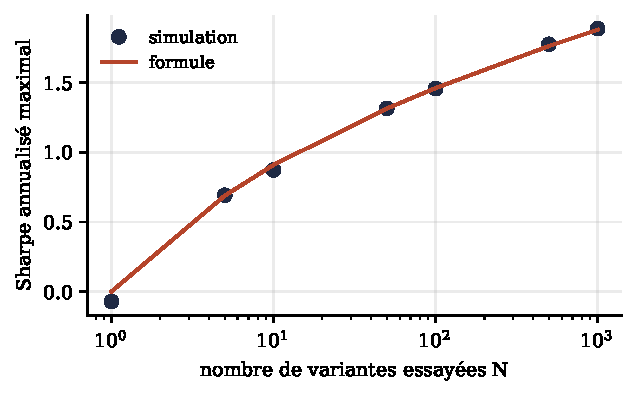
\includegraphics[width=0.55\textwidth]{ch16/max_sharpe.pdf}
\caption{Sharpe annualisé maximal attendu parmi $N$ stratégies sans avantage, sur 3 ans de données quotidiennes.}
\label{c16:fig:emax}
\end{figure}

\paragraph{Lecture.} En essayant 100 paires ou 100 réglages sur trois ans de données, on obtient \emph{en moyenne} un Sharpe de $1{,}46$ sans aucun avantage réel. C'est l'ordre de grandeur des performances publiées sur les réseaux sociaux. \citet{harvey2016} tirent la même conclusion pour la recherche académique : après des centaines de facteurs testés, un seuil de $t$-statistique de 2 est trop faible ; ils recommandent au moins 3.

% =====================================================================
\section{Le ratio de Sharpe probabiliste et déflaté}
% =====================================================================

\begin{definition}[PSR]
Le \emph{ratio de Sharpe probabiliste} d'un Sharpe estimé $\widehat{SR}$ sur $T$ périodes par rapport à un seuil $SR^\ast$ est
\[
\text{PSR}(SR^\ast) = \Phi\!\left(\frac{(\widehat{SR} - SR^\ast)\sqrt{T-1}}{\sqrt{1 - \gamma_3\widehat{SR} + \frac{\gamma_4-1}{4}\widehat{SR}^2}}\right).
\]
C'est la probabilité, compte tenu de l'erreur d'estimation (proposition~\ref{c16:prop:sese}), que le vrai Sharpe dépasse $SR^\ast$.
\end{definition}

\begin{definition}[DSR, \citet{bailey2014dsr}]
Le \emph{ratio de Sharpe déflaté} de la meilleure de $N$ variantes est le PSR calculé avec, pour seuil, le maximum espéré de la proposition~\ref{c16:prop:emax} : $\text{DSR} = \text{PSR}\big(\E[\max_n \widehat{SR}_n]\big)$, où $V$ est estimée par la variance des Sharpe des $N$ variantes essayées.
\end{definition}

\begin{intuition}
Le DSR répond à la question : \og ma meilleure variante bat-elle ce que le hasard m'aurait donné en essayant autant de variantes ?\fg. Un DSR supérieur à 0,95 signifie qu'il y a moins de 5\,\% de chances que le résultat ne soit que le meilleur tirage d'une loterie.
\end{intuition}

\begin{pitfall}
Le DSR exige de connaître $N$, le nombre de variantes \emph{réellement} essayées, y compris celles qu'on a abandonnées en cours de route, les autres paires regardées, les autres périodes testées. C'est pourquoi le fichier \texttt{CLAUDE.md} du dépôt impose de consigner le nombre de variantes avec chaque résultat. Si les variantes sont très corrélées (deux seuils voisins), $N$ \og effectif\fg{} est plus petit que le nombre brut : le DSR calculé avec le nombre brut est alors conservateur.
\end{pitfall}

% =====================================================================
\section{Organiser les données : formation, validation, test}
% =====================================================================

\subsection{Le découpage}

\begin{center}\small
\begin{tabular}{p{3.0cm}p{9.8cm}}
\toprule
Période & Usage \\
\midrule
Formation & Estimer les paramètres du modèle ($\beta$, moyenne, écart-type, demi-vie) et sélectionner les paires. \\
Validation & Choisir les réglages (seuil d'entrée, fenêtre) parmi un petit nombre de variantes déclarées à l'avance. \\
Test & Mesurer la performance \emph{une seule fois}, à la fin. Un test regardé deux fois devient une validation. \\
\bottomrule
\end{tabular}
\end{center}

\subsection{La validation glissante (\emph{walk-forward})}

Les marchés changent : un découpage unique donne un seul point de mesure. La validation glissante répète le cycle \og former sur $[t-F, t)$, trader sur $[t, t+H)$\fg{} en avançant $t$ de $H$ à chaque étape, puis concatène les périodes de trading. Chaque jour de la courbe finale est hors échantillon par rapport aux paramètres utilisés ce jour-là. C'est la structure de \citet{gatev2006} (formation de 12 mois, trading de 6 mois, avec chevauchement des cohortes, chapitre~6).

\subsection{Purge et embargo}

Quand l'étiquette d'une observation dépend du futur (par exemple \og l'écart se sera-t-il refermé dans 10 jours ?\fg{} au chapitre~11), les observations de formation proches de la frontière avec le test contiennent de l'information sur le test. \citet{lopezdeprado2018} recommande de \emph{purger} ces observations et d'ajouter un \emph{embargo} (quelques jours écartés après chaque période de test).

% =====================================================================
\section{Optimiser sans se tromper : expérience complète}
% =====================================================================

\begin{codebox}[ — E4, optimisation d'une grille de 50 variantes]
\textbf{Grille :} seuils d'entrée $\{1; 1{,}5; 2; 2{,}5; 3\}$, fenêtres du \emph{z-score} $\{20; 40; 60; 120; 250\}$ jours, sorties à $z=0$ ou $|z| = 0{,}5$ ; coûts 5 pb par jambe. \textbf{Protocole :} 60 mondes de 1\,750 jours par scénario ; on choisit la meilleure variante sur la première moitié, on la mesure sur la seconde. Sharpe annualisés moyens :
\begin{center}\small
\begin{tabular}{lcc}
\toprule
 & Sans avantage ($\varphi=1$) & Avec avantage ($\varphi=0{,}97$) \\
\midrule
Meilleure variante, dans l'échantillon & 0,96 & 1,64 \\
Meilleure variante, hors échantillon & $-0{,}03$ & 1,02 \\
Variante médiane, hors échantillon & $-0{,}10$ & 0,83 \\
DSR moyen de la meilleure variante & 0,52 & 0,85 \\
Part des mondes où DSR $>0{,}95$ & 0\,\% & 15\,\% \\
\bottomrule
\end{tabular}
\end{center}
\end{codebox}

\paragraph{Lecture.} Dans le monde sans avantage, l'optimisation affiche un Sharpe de près de 1 qui disparaît entièrement hors échantillon, et le DSR ne dépasse jamais 0,95 : il ne se laisse pas tromper. Dans le monde avec avantage, l'optimisation surestime aussi le Sharpe (1,64 contre 1,02 hors échantillon), mais la meilleure variante reste supérieure à la médiane : choisir n'était pas inutile. En revanche, le DSR ne valide la stratégie que dans 15\,\% des mondes : avec trois ans et demi de données et 50 variantes, un avantage réel de Sharpe 1 est difficile à prouver. C'est le prix de l'honnêteté statistique ; la solution est d'essayer moins de variantes, d'avoir plus de données, ou d'accumuler une période de \emph{paper trading}.

% =====================================================================
\section{La probabilité de surapprentissage (PBO)}
% =====================================================================

\subsection{La validation croisée combinatoire symétrique}

\citet{bailey2017pbo} proposent de mesurer directement si \og choisir la meilleure variante\fg{} est une procédure fiable sur les données disponibles.

\begin{enumerate}
\item On range les gains des $M$ variantes dans une matrice $T\times M$ et on découpe les $T$ dates en $S$ blocs consécutifs ($S$ pair).
\item Pour chacune des $\binom{S}{S/2}$ façons de choisir la moitié des blocs comme échantillon de sélection (le reste servant de test) : on retient la variante $n^\ast$ de meilleur Sharpe dans la sélection, puis on calcule son rang relatif $\omega \in (0,1)$ parmi les $M$ variantes sur le test, et le \emph{logit} $\lambda = \ln\big(\omega/(1-\omega)\big)$.
\item La PBO est la proportion des découpages pour lesquels $\lambda \le 0$, c'est-à-dire où la meilleure variante en sélection finit dans la moitié inférieure en test.
\end{enumerate}

\begin{intuition}
Si la sélection n'apprend que du bruit, la meilleure variante d'une moitié des données n'a aucune raison d'être bonne sur l'autre moitié : elle tombe sous la médiane une fois sur deux, et la PBO vaut environ $0{,}5$. Si la sélection capte quelque chose de réel, la PBO tombe vers 0.
\end{intuition}

\begin{codebox}[ — E5, PBO des grilles de E4 ($S = 12$ blocs, 924 découpages)]
PBO moyenne : $0{,}38$ dans le monde sans avantage, $0{,}30$ dans le monde avec avantage. Les tests unitaires du module vérifient le comportement de référence : sur 30 variantes de pur bruit indépendantes, PBO comprise entre $0{,}25$ et $0{,}75$ ; si une variante a un vrai avantage, PBO inférieure à $0{,}05$.
\end{codebox}

\begin{figure}[h]
\centering
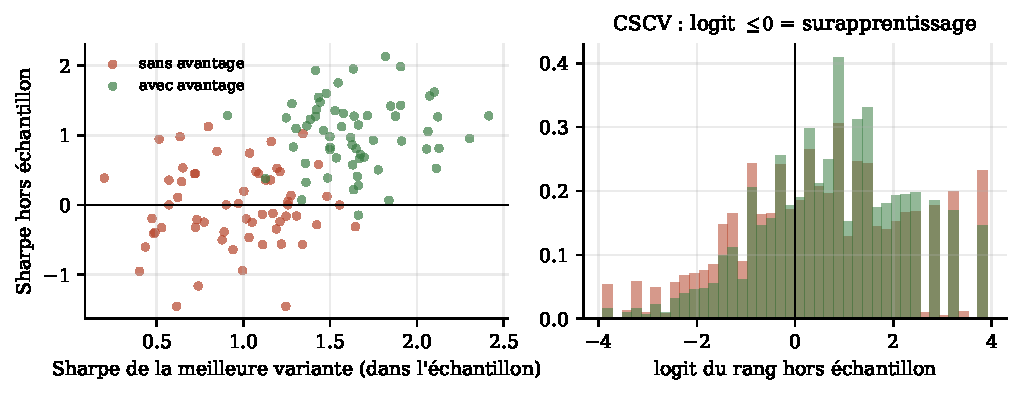
\includegraphics[width=0.95\textwidth]{ch16/is_oos_pbo.pdf}
\caption{À gauche, Sharpe de la meilleure variante dans l'échantillon contre hors échantillon (E4). À droite, distribution des logits de la CSCV (E5) : la masse à gauche de zéro est la PBO.}
\label{c16:fig:pbo}
\end{figure}

\paragraph{Lecture.} Dans le monde sans avantage, la PBO ($0{,}38$) est inférieure à $0{,}5$ alors que la meilleure variante ne gagne rien hors échantillon. La raison : la PBO mesure un \emph{classement relatif}. Les variantes à seuil élevé traitent moins et paient moins de coûts ; elles sont régulièrement \og moins mauvaises\fg{} que les autres, et cette régularité est réelle. La PBO dit donc si la sélection est reproductible, pas si la stratégie gagne. Elle se lit toujours avec le niveau du Sharpe hors échantillon et le DSR.

% =====================================================================
\section{Un moteur sans anticipation}
% =====================================================================

Le module \texttt{arbhub.backtest.engine} implémente les règles de ce chapitre en trois fonctions.

\begin{lstlisting}[language=Python]
from arbhub.backtest.engine import rolling_zscore, zscore_positions, pair_backtest
from arbhub.backtest.metrics import annualized_sharpe, deflated_sharpe, max_drawdown

z = rolling_zscore(y - beta * x, window=60)       # n'utilise que s[t-59..t]
q = zscore_positions(z, entry=2.0, exit=0.0, stop=4.0)
res = pair_backtest(y, x, beta, q, cost_bps=5)    # gain[t+1] = q[t] * dS ; couts en t
print(annualized_sharpe(res.net), max_drawdown(res.net), res.n_trades)
\end{lstlisting}

Les tests (\texttt{tests/test\_backtest.py}) vérifient : l'absence d'anticipation (modification des données futures) ; l'égalité du P\&L avec la formule manuelle~\eqref{c16:eq:pnl} ; des coûts payés uniquement lors des changements de position et égaux au notionnel échangé multiplié par le coût ; le fonctionnement du stop-loss ; l'égalité du \emph{z-score} glissant avec un calcul naïf ; et les propriétés de référence du PSR, du DSR et de la PBO.

% =====================================================================
\section{Les coûts, encore}
% =====================================================================

Un \emph{backtest} sans coûts est inutilisable (chapitres~1, 6 et~12). Le modèle minimal à déclarer, par jambe et par transaction : commission, demi-fourchette achat-vente, glissement estimé ; et, par jour de détention : coût d'emprunt des titres vendus à découvert, financement des positions à crédit, \emph{funding} des perpétuels (chapitre~14). Une bonne pratique est de publier le \emph{coût de rentabilité nulle} : le coût par jambe pour lequel le gain net devient nul. S'il est inférieur au double de vos coûts estimés, la stratégie n'a pas de marge de sécurité.

% =====================================================================
\section{Ce que la théorie apporte, et ses limites}
% =====================================================================

\paragraph{Apports.} Des ordres de grandeur sur ce qu'un \emph{backtest} peut prouver (il faut des années pour distinguer un Sharpe de 1 du hasard), une correction explicite du nombre d'essais, et un moteur dont l'absence d'anticipation est garantie par des tests.

\paragraph{Limites.} Le DSR et la PBO supposent que le passé est représentatif du futur ; aucun ne protège contre un changement de régime. Le nombre d'essais est souvent mal connu. Enfin, un \emph{backtest} ne capture pas l'exécution réelle (files d'attente, exécutions partielles, rejets) : seule une période de \emph{paper trading} puis de petite taille réelle mesure la stratégie telle qu'elle sera traitée (chapitre~18).

% =====================================================================
\section{Fiche à recopier au tableau blanc}
% =====================================================================

\begin{whiteboard}
\begin{itemize}[leftmargin=1.2em]
\item \textbf{Sans anticipation :} $\text{gain}_{t+1} = q_t(S_{t+1}-S_t)$, $q_t$ fonction des seules données $\le t$ ; test automatique : modifier le futur ne change pas le passé.
\item \textbf{Trois biais :} anticipation, survie (garder les radiés), sélection (compter les essais).
\item \textbf{Erreur-type du Sharpe :} $\sqrt{(1+SR^2/2)/T}$ par période ; annualisé $\approx 1/\sqrt{\text{années}}$.
\item \textbf{Maximum de $N$ Sharpe nuls :} $\approx\sqrt V\big((1-\gamma)\Phi^{-1}(1-\tfrac1N) + \gamma\Phi^{-1}(1-\tfrac{1}{Ne})\big)$, croît comme $\sqrt{2\ln N/T}$.
\item \textbf{PSR :} $\Phi\big((\widehat{SR}-SR^\ast)\sqrt{T-1}/\sqrt{1-\gamma_3\widehat{SR}+\frac{\gamma_4-1}{4}\widehat{SR}^2}\big)$ ; \textbf{DSR :} PSR avec $SR^\ast = \E[\max]$.
\item \textbf{PBO :} proportion des découpages CSCV où la meilleure variante en sélection finit sous la médiane en test.
\item \textbf{Découpage :} formation, validation, test regardé une seule fois ; \emph{walk-forward} ; purge et embargo.
\end{itemize}
\end{whiteboard}

% =====================================================================
\section{Exercices}
% =====================================================================

\begin{exercise}
Une stratégie affiche un Sharpe annualisé de $1{,}5$ sur deux ans de données quotidiennes. Calculez l'erreur-type et un intervalle de confiance à 95\,\% du vrai Sharpe. Combien d'années faudrait-il pour que la borne basse dépasse $0{,}5$ ?
\end{exercise}

\begin{exercise}
Vous avez testé 200 paires sur 4 ans et la meilleure affiche un Sharpe de $2{,}1$. En supposant $V = 1/T$, calculez le maximum espéré sous l'hypothèse nulle. Le résultat est-il impressionnant ?
\end{exercise}

\begin{exercise}
Démontrez l'approximation $\E[\max]\approx\sqrt{2V\ln N}$ pour $N$ grand, en utilisant $\Phi^{-1}(1-p)\approx\sqrt{2\ln(1/p)}$ pour $p$ petit.
\end{exercise}

\begin{exercise}[à coder]
Écrivez une fonction \texttt{walk\_forward(y, x, F, H)} qui réestime $\beta$, la moyenne et l'écart-type sur chaque fenêtre de formation de $F$ jours et trade les $H$ jours suivants. Ajoutez-lui un test d'absence d'anticipation dans \texttt{tests/}.
\end{exercise}

\begin{exercise}[à coder]
Remplacez dans E2 les rendements i.i.d. par des gains autocorrélés (AR(1) de paramètre $0{,}3$). De combien l'écart-type du Sharpe estimé augmente-t-il ? Comparez avec un \emph{bootstrap} par blocs de 20 jours.
\end{exercise}

\begin{exercise}[données réelles]
Reprenez votre meilleure paire du chapitre~7. Notez honnêtement combien de paires et de réglages vous avez essayés, puis calculez son DSR. Que concluez-vous ?
\end{exercise}

% =====================================================================
\section{Pour aller plus loin}
% =====================================================================

\begin{toread}
\begin{itemize}[leftmargin=1.2em]
\item \citet{bailey2014dsr} : sections 2 et 3 pour le maximum espéré et le DSR, avec un exemple numérique complet.
\item \citet{bailey2017pbo} : section 2 pour l'algorithme CSCV, section 4 pour l'interprétation de la PBO.
\item \citet{lo2002} : la loi asymptotique du Sharpe, y compris pour des rendements autocorrélés.
\item \citet{harvey2016} : sections sur les corrections de Bonferroni, Holm et Benjamini-Hochberg-Yekutieli.
\item \citet{white2000} : le \emph{reality check}, test formel de la meilleure parmi plusieurs stratégies.
\item \citet{lopezdeprado2018} : chapitres 7 (validation croisée purgée), 11 (dangers du \emph{backtest}) et 14 (statistiques de \emph{backtest}).
\end{itemize}
\end{toread}

\section{Scripts du chapitre}
\noindent\texttt{code/ch16/ch16\_backtest.py} : E1 (figure~\ref{c16:fig:lookahead}), E2, E3 (figure~\ref{c16:fig:emax}), E4–E5 (figure~\ref{c16:fig:pbo}), E6. Modules : \texttt{src/arbhub/backtest/engine.py}, \texttt{metrics.py} ; tests : \texttt{tests/test\_backtest.py}.

% =====================================================================
\chapter{Risque et limites de l'arbitrage}
\label{ch:17}
% =====================================================================

\section{Objectifs et organisation du chapitre}

\paragraph{Objectifs.} Une stratégie d'arbitrage statistique gagne souvent un peu et perd rarement beaucoup. Le risque se concentre dans quelques épisodes : une paire qui se rompt, un écart qui s'élargit avant de converger, une foule d'arbitragistes qui liquident en même temps. À la fin du chapitre, vous saurez : (1) dimensionner une position avec le critère de Kelly et comprendre pourquoi on n'en utilise qu'une fraction ; (2) choisir et calibrer des protections contre la rupture d'une paire ; (3) expliquer, chiffres à l'appui, pourquoi un arbitrage \og certain\fg{} peut ruiner celui qui le porte ; (4) mesurer ce que vaut réellement la diversification entre paires ; (5) recenser les risques non statistiques (plateforme, contrepartie, réglementation, règles des \emph{prop firms}) et fixer des limites de risque.

\paragraph{Code.}\sloppy \texttt{code/ch17/ch17\_risk.py} (expériences E1 à E4) ; module \texttt{src/arbhub/risk/sizing.py} et ses tests \texttt{tests/test\_risk.py}.

% =====================================================================
\section{Combien miser ? Le critère de Kelly}
% =====================================================================

\subsection{Croissance logarithmique}

On investit à chaque période une fraction $f$ de sa richesse (le \emph{levier}) dans une stratégie de rendement $r_t$, d'espérance $\mu$ et de variance $\sigma^2$ par période. La richesse évolue selon $W_{t+1} = W_t(1 + f r_t)$, donc après $T$ périodes
\[
\ln W_T = \ln W_0 + \sum_{t=1}^{T}\ln(1 + f r_t).
\]
Par la loi des grands nombres, le taux de croissance $\frac1T\ln(W_T/W_0)$ converge vers $g(f) = \E[\ln(1+fr)]$. Le critère de Kelly \citep{kelly1956} choisit $f$ pour maximiser ce taux.

\begin{proposition}[Kelly en temps continu, \citet{thorp2006}]\label{c17:prop:kelly}
Pour des rendements petits, $g(f) \approx f\mu - \tfrac12 f^2\sigma^2$, maximal en
\[
f^\star = \frac{\mu}{\sigma^2}, \qquad g(f^\star) = \frac{\mu^2}{2\sigma^2} = \frac{SR^2}{2},
\]
où $SR = \mu/\sigma$ est le Sharpe par période. De plus $g(2f^\star) = 0$ : avec le double du levier de Kelly, la richesse ne croît plus.
\end{proposition}
\begin{proof}
Le développement $\ln(1+u) = u - u^2/2 + O(u^3)$ appliqué à $u = fr$ donne $\E[\ln(1+fr)] \approx f\E[r] - \tfrac12 f^2\E[r^2]$. Pour des rendements par période petits, $\E[r^2] = \sigma^2 + \mu^2 \approx \sigma^2$. La fonction $g(f) = f\mu - \tfrac12 f^2\sigma^2$ est une parabole tournée vers le bas ; sa dérivée $\mu - f\sigma^2$ s'annule en $f^\star = \mu/\sigma^2$, et $g(f^\star) = \mu^2/\sigma^2 - \tfrac12\mu^2/\sigma^2 = \mu^2/(2\sigma^2)$. Enfin $g(2f^\star) = 2\mu^2/\sigma^2 - \tfrac12\cdot4\mu^2/\sigma^2 = 0$.
\end{proof}

\begin{intuition}
La croissance est une colline. Jusqu'au sommet ($f^\star$), plus de levier fait monter plus vite. Après le sommet, chaque unité de levier supplémentaire ajoute plus de volatilité qu'elle n'ajoute de rendement, et la volatilité \emph{détruit} la croissance : perdre 50\,\% puis gagner 50\,\% laisse 75\,\% du capital. À deux fois le sommet, on est revenu au niveau de la mer : en moyenne arithmétique on gagne, en médiane on stagne.
\end{intuition}

\subsection{Kelly en pratique}

\begin{codebox}[ — E1, stratégie de Sharpe annuel 1 (rendement 10\,\%, volatilité 10\,\% sans levier), 4\,000 trajectoires de 10 ans]
Le levier de Kelly vaut $f^\star = 0{,}10/0{,}10^2 = 10$, soit une volatilité de 100\,\% par an.
\begin{center}\small
\setlength{\tabcolsep}{4pt}
\begin{tabular}{rrcccc}
\toprule
Fraction & Levier & Croissance & P(perte & P(drawdown & Drawdown \\
de Kelly & & médiane & à 10 ans) & $>50\,\%$) & médian \\
\midrule
0,10 & 1 & 10,0\,\%/an & 0,2\,\% & 0\,\% & 15,8\,\% \\
0,25 & 2,5 & 24,6\,\%/an & 0,3\,\% & 9,1\,\% & 36,1\,\% \\
0,50 & 5 & 45,9\,\%/an & 0,9\,\% & 86,5\,\% & 61,6\,\% \\
1,00 & 10 & 66,0\,\%/an & 5,4\,\% & 100\,\% & 89,6\,\% \\
1,50 & 15 & 46,5\,\%/an & 21,6\,\% & 100\,\% & 98,5\,\% \\
2,00 & 20 & $-0{,}8$\,\%/an & 50,4\,\% & 100\,\% & 99,9\,\% \\
\bottomrule
\end{tabular}
\end{center}
\textbf{Erreur d'estimation :} si l'on estime $f^\star$ sur 3 ans d'historique de cette même stratégie, l'estimation médiane est juste ($10{,}0$), mais 10\,\% des estimations sont sous $2{,}4$ et 10\,\% au-dessus de $17{,}5$ ; dans 4,2\,\% des cas on estime plus du double du vrai $f^\star$ (zone de croissance négative), et dans 4,7\,\% un $f^\star$ négatif.
\end{codebox}

\begin{figure}[h]
\centering
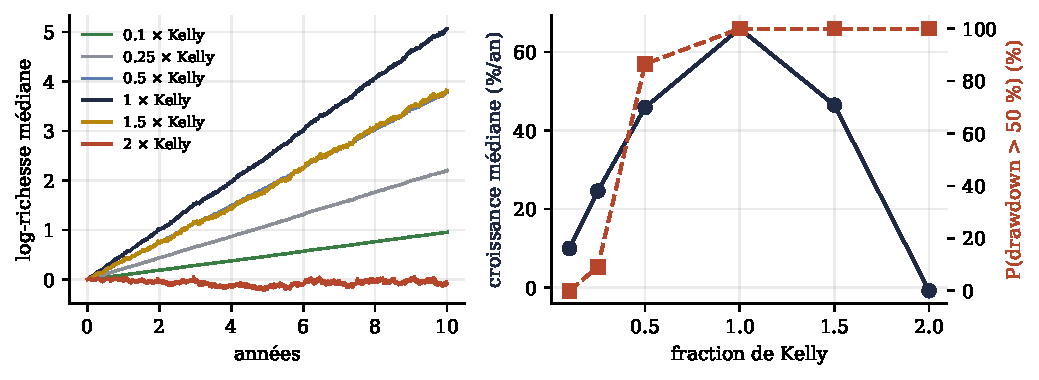
\includegraphics[width=0.95\textwidth]{ch17/kelly.pdf}
\caption{À gauche, log-richesse médiane selon la fraction de Kelly (les courbes à 0,5 et 1,5 Kelly se superposent : la croissance est symétrique autour du sommet). À droite, croissance médiane et probabilité de subir un drawdown de plus de 50\,\%.}
\label{c17:fig:kelly}
\end{figure}

\paragraph{Lecture.} Kelly maximise la croissance \emph{à long terme} en acceptant des drawdowns que presque personne ne supporte (90\,\% en médiane). La croissance est symétrique autour de $f^\star$ (0,5 et 1,5 Kelly croissent au même rythme), mais le risque ne l'est pas : la sur-estimation est bien plus coûteuse que la sous-estimation. Comme $f^\star$ est estimé avec une erreur énorme, la pratique professionnelle est d'utiliser entre un dixième et un quart de Kelly. Pour une stratégie de paires, rappelez-vous en outre que le Sharpe d'un \emph{backtest} est surestimé (chapitre~16) : le Kelly calculé sur un \emph{backtest} est doublement trop grand.

\subsection{Ciblage de volatilité}

Une alternative simple consiste à fixer une volatilité cible $\sigma^\ast$ (par exemple 10\,\% par an) et à dimensionner à chaque date
\[
w_t = \min\!\Big(\frac{\sigma^\ast}{\hat\sigma_t},\ L_{\max}\Big),
\]
où $\hat\sigma_t$ est la volatilité du P\&L par unité de position estimée sur une fenêtre passée, et $L_{\max}$ un levier plafond. C'est la fonction \texttt{vol\_target\_weights} du module ; son test vérifie qu'elle n'utilise que le passé et qu'elle atteint la cible sur des données stables. Le ciblage réduit la taille quand la volatilité monte, ce qui protège partiellement des épisodes de crise, mais avec un retard égal à la fenêtre d'estimation.

% =====================================================================
\section{Se protéger de la rupture d'une paire}
% =====================================================================

Le chapitre~1 a montré qu'une paire rompue transforme une règle de retour à la moyenne en machine à accumuler des pertes. On compare ici cinq protections.

\begin{description}
\item[Stop-loss en $z$.] On ferme si $|z_t| > z_{\text{stop}}$ (3 ou 4), et l'on ne rouvre que si $|z|$ redescend sous le seuil d'entrée.
\item[Stop-loss en durée.] On ferme si la position est ouverte depuis plus de trois demi-vies : un écart qui revient à la moyenne devrait s'être largement refermé dans ce délai (chapitre~5).
\item[Alarme CUSUM.] On surveille les innovations $e_t = s_t - \hat\varphi s_{t-1}$, qui doivent rester un bruit blanc de moyenne et d'écart-type connus si la relation est stable. Le CUSUM de \citet{page1954} cumule les écarts standardisés $z_t = (e_t - m)/d$ au-delà d'une marge $k$ :
\[
S^+_t = \max(0, S^+_{t-1} + z_t - k), \qquad S^-_t = \max(0, S^-_{t-1} - z_t - k),
\]
et déclenche une alarme dès que $S^+_t$ ou $S^-_t$ dépasse $h$. Une alarme retire la paire.
\item[$\hat\varphi$ glissant.] On suspend la paire tant que $\hat\varphi$ estimé sur les 120 derniers jours dépasse $0{,}98$.
\end{description}

\begin{intuition}
Le CUSUM est un compteur de \og petits mauvais signes\fg. Un jour légèrement anormal ne fait rien ($k$ absorbe le bruit), mais une série de jours anormaux dans le même sens s'accumule jusqu'à l'alarme. C'est la logique du contrôle qualité industriel, pour lequel il a été inventé : une machine déréglée produit des pièces un peu trop grandes, jour après jour.
\end{intuition}

\begin{codebox}[ — E2, cinq protections, 300 mondes par scénario]
\textbf{Protocole :} écart AR(1) avec $\varphi = 0{,}9$, formation de 500 jours, trading de 1\,000 jours, règle $|z|>2$, coûts 5 pb. Scénario \og rupture\fg{} : au 400\textsuperscript{e} jour de trading, l'écart devient une marche aléatoire avec une légère dérive. CUSUM avec $k = 0{,}5$ et $h = 10$. \textbf{Gain moyen (quantile 5\,\%) :}
\begin{center}\small
\begin{tabular}{lcc}
\toprule
Protection & Relation stable & Rupture \\
\midrule
Aucune & 63,7 (33,1) & $-22{,}2$ ($-70{,}5$) \\
Stop $|z| > 3$ & 58,7 (32,3) & 20,0 (0,3) \\
Stop $|z| > 4$ & 63,4 (33,1) & 20,0 ($-2{,}1$) \\
Stop en durée (3 demi-vies) & 54,6 (26,6) & 19,3 (0,0) \\
CUSUM & 60,8 (29,6) & 23,6 (4,9) \\
$\hat\varphi$ glissant & 63,7 (33,1) & $-4{,}1$ ($-37{,}0$) \\
\bottomrule
\end{tabular}
\end{center}
\textbf{CUSUM :} fausse alarme dans 7\,\% des mondes stables ; alarme après la rupture dans 96,7\,\% des mondes qui rompent, avec un délai médian de 53 jours.
\end{codebox}

\begin{figure}[h]
\centering
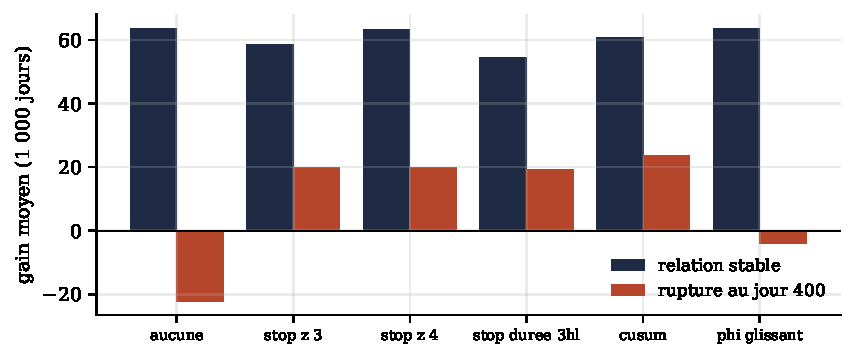
\includegraphics[width=0.8\textwidth]{ch17/protections_rupture.pdf}
\caption{Gain moyen selon la protection, avec une relation stable et avec une rupture au 400\textsuperscript{e} jour.}
\label{c17:fig:protect}
\end{figure}

\paragraph{Lecture.} (1) Le stop à $|z|>4$ est presque gratuit quand la relation est stable (63,4 contre 63,7) et transforme une perte moyenne de 22 en gain de 20 quand elle rompt : c'est la meilleure assurance par unité de coût. (2) Le stop à 3 coûte davantage (il coupe des écarts qui seraient revenus). (3) Le CUSUM offre la meilleure protection en cas de rupture et ne coûte que 3 en monde stable, au prix d'un calibrage (avec $k = 0{,}25$ et $h = 8$, un premier essai, il déclenchait à tort dans 94\,\% des mondes stables). (4) Le $\hat\varphi$ glissant ne déclenche jamais à tort mais réagit trop lentement : il faut 120 jours pour que l'estimation reflète le nouveau régime. Dans la pratique, on combine un stop en $z$ (protection immédiate) et un indicateur statistique (pour retirer durablement la paire).

\begin{pitfall}
Ces protections ont été évaluées dans un monde où l'on connaît la date de rupture. Dans la réalité, chaque déclenchement est ambigu : écart extrême mais temporaire, ou rupture ? Le stop vend souvent au pire moment, juste avant la convergence. Calibrer les seuils sur l'historique d'une paire est un nouveau choix de paramètres, à compter dans le nombre d'essais (chapitre~16).
\end{pitfall}

% =====================================================================
\section{Les limites de l'arbitrage}
% =====================================================================

\subsection{L'argument de Shleifer et Vishny}

\citet{shleifer1997} partent d'un constat : l'arbitrage est réalisé par peu d'acteurs spécialisés qui utilisent un capital emprunté (marge, levier) ou délégué (investisseurs d'un fonds). Quand un écart s'élargit avant de converger, l'arbitragiste subit des pertes latentes ; ses prêteurs exigent de la marge supplémentaire, ses investisseurs retirent leur argent, et il doit liquider \emph{au moment où l'opportunité est la meilleure}. Sa vente élargit encore l'écart. L'arbitrage est donc le plus contraint précisément quand il serait le plus utile. \citet{brunnermeier2009} formalisent cette spirale entre liquidité de financement et liquidité de marché ; \citet{mitchell2010} documentent des écarts d'arbitrage qui sont restés ouverts des mois en 2008, faute de capital pour les fermer.

\subsection{Expérience : un arbitrage certain qui ruine}

\begin{codebox}[ — E3, spirale de marge]
\textbf{Protocole :} un écart vaut 2 aujourd'hui et vaudra 0 \emph{avec certitude} dans 120 jours (comme la base d'un future à l'échéance). Dans la moitié des cas, une crise de liquidité l'élargit en moyenne de 3 pendant les 20 premiers jours. L'arbitragiste vend une taille $L$ d'écart par unité de capital ; il est liquidé si sa perte latente dépasse 75\,\% de son capital. 20\,000 trajectoires, les mêmes pour chaque taille. \textbf{Résultats :}
\begin{center}\small
\begin{tabular}{rcccc}
\toprule
Taille $L$ & Gain si l'on tient & P(liquidation) & P(liquidation \textbar{} crise) & Gain moyen réalisé \\
\midrule
0,05 & 0,10 & 0\,\% & 0\,\% & 0,100 \\
0,10 & 0,20 & 0\,\% & 0\,\% & 0,200 \\
0,15 & 0,30 & 1,3\,\% & 2,6\,\% & 0,286 \\
0,20 & 0,40 & 10,9\,\% & 21,5\,\% & 0,271 \\
0,30 & 0,60 & 35,1\,\% & 66,1\,\% & 0,110 \\
0,50 & 1,00 & 56,8\,\% & 92,6\,\% & $-0{,}041$ \\
1,00 & 2,00 & 74,6\,\% & 98,7\,\% & $-0{,}175$ \\
\bottomrule
\end{tabular}
\end{center}
\end{codebox}

\begin{figure}[h]
\centering
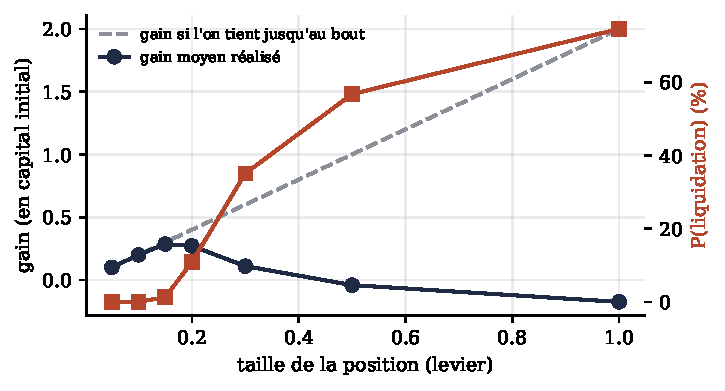
\includegraphics[width=0.6\textwidth]{ch17/spirale_marge.pdf}
\caption{Un arbitrage dont la convergence est certaine : le gain promis croît avec la taille, le gain réalisé passe par un maximum puis devient négatif, car la probabilité d'être liquidé avant la convergence explose.}
\label{c17:fig:margin}
\end{figure}

\paragraph{Lecture.} La convergence est garantie, et pourtant un arbitragiste trop levé perd de l'argent en moyenne. Le gain espéré est maximal pour une taille modeste ($L \approx 0{,}15$), bien en dessous de ce que suggère le \og gain certain\fg. La leçon s'applique directement aux stratégies de base et de \emph{funding} du chapitre~14 : la convergence à l'échéance ne protège pas d'une liquidation avant l'échéance. Le levier se choisit en fonction du \emph{pire élargissement plausible}, pas du gain attendu.

\subsection{La foule : août 2007}

\citet{khandanilo2011} analysent la semaine du 6 août 2007, pendant laquelle de nombreux fonds d'arbitrage statistique sur actions ont subi des pertes très inhabituelles, suivies d'un rebond partiel. Leur explication : beaucoup de fonds détenaient des portefeuilles semblables (mêmes facteurs, mêmes signaux) ; le débouclage rapide de l'un d'eux a fait bouger les prix contre tous les autres, ce qui a déclenché d'autres débouclages. Une stratégie est d'autant plus exposée qu'elle est populaire : le \emph{pairs trading} sur grandes capitalisations est l'une des stratégies quantitatives les plus répandues.

% =====================================================================
\section{Ce que vaut la diversification}
% =====================================================================

\begin{proposition}\label{c17:prop:div}
Soit un portefeuille équipondéré de $N$ paires, chacune de volatilité $\sigma$, avec une corrélation commune $\rho$ entre deux paires quelconques. Sa volatilité vaut
\[
\sigma_P = \sigma\sqrt{\frac1N + \rho\Big(1 - \frac1N\Big)}, \qquad\text{et}\qquad N_{\text{eff}} = \frac{\sigma^2}{\sigma_P^2} = \frac{N}{1 + (N-1)\rho}.
\]
\end{proposition}
\begin{proof}
Avec des poids $1/N$, $\Var\big(\frac1N\sum_i r_i\big) = \frac1{N^2}\big(\sum_i\Var(r_i) + \sum_{i\ne j}\Cov(r_i,r_j)\big) = \frac{1}{N^2}\big(N\sigma^2 + N(N-1)\rho\sigma^2\big) = \sigma^2\big(\frac1N + \rho\frac{N-1}{N}\big)$. Le nombre effectif est le nombre de paires indépendantes qui donneraient la même volatilité : $\sigma^2/N_{\text{eff}} = \sigma_P^2$.
\end{proof}

\begin{codebox}[ — E4, 20 paires]
\textbf{Volatilité relative et nombre effectif de paires :} $\rho = 0$ : $0{,}224$ ($N_{\text{eff}} = 20$) ; $\rho = 0{,}05$ : $0{,}312$ ($10{,}3$) ; $\rho = 0{,}1$ : $0{,}381$ ($6{,}9$) ; $\rho = 0{,}3$ : $0{,}579$ ($3{,}0$) ; $\rho = 0{,}6$ : $0{,}787$ ($1{,}6$). \textbf{Crise :} 20 paires de Sharpe annuel $1{,}6$ chacune, corrélation $0{,}05$ en temps normal ; une crise de 10 jours fait monter la corrélation à $0{,}6$ et inverse le rendement. Sur 10 ans, le drawdown maximal médian passe de $9{,}2$ à $34{,}1$ écarts-types quotidiens du portefeuille.
\end{codebox}

\paragraph{Lecture.} Une corrélation de seulement $0{,}05$ entre paires divise par deux le bénéfice de la diversification. Et la corrélation n'est pas stable : elle monte précisément pendant les crises, quand tous les arbitragistes liquident ensemble. Un portefeuille de 20 paires calibré sur la volatilité de temps normal subit en crise un drawdown près de quatre fois plus grand que prévu. Il faut donc dimensionner sur la volatilité \emph{de crise}, et diversifier entre familles de stratégies (actions, base, \emph{funding}, différents horizons) plutôt qu'entre paires d'une même famille.

% =====================================================================
\section{Les risques non statistiques}
% =====================================================================

\begin{description}
\item[Plateforme et contrepartie.] Une plateforme peut tomber en panne, geler les retraits ou faire faillite. Pour l'arbitrage inter-plateformes, le capital immobilisé sur chaque plateforme est exposé à ce risque, qui ne figure dans aucun \emph{backtest}. Règle : ne laisser sur une plateforme que la marge nécessaire, et plafonner l'exposition par contrepartie.
\item[Courtier et règles d'exécution.] Les CFD sont des contrats avec votre courtier, qui peut modifier les écarts, les heures, la marge ou refuser certains styles de trading. Le moteur \texttt{atjte} prévoit des plages d'interdiction (\emph{blackouts}) et des contrôles de marge à cet effet \citep{atjte}.
\item[Vente à découvert.] Les titres vendus doivent être empruntés ; le coût d'emprunt peut monter brutalement et le prêteur peut rappeler les titres, forçant à racheter.
\item[Opérations sur titres.] Dividendes, divisions, fusions, offres publiques : chacune peut créer un faux signal ou une rupture réelle.
\item[Réglementation et fiscalité.] Restrictions de vente à découvert en période de crise, régime fiscal des CFD et des cryptoactifs, obligations déclaratives des comptes à l'étranger.
\item[\emph{Prop firms}.] Les règles des \emph{prop firms} interdisent en général l'arbitrage de latence, la couverture croisée entre comptes et l'exploitation de défauts de cotation \citep{nexusfi}. Une stratégie d'arbitrage inter-plateformes déployée sur un compte de \emph{prop firm} risque l'annulation des gains et la fermeture du compte. Ces stratégies relèvent du capital propre.
\item[Risque opérationnel.] Bogues, erreurs de saisie (un ratio mal tapé), double lancement d'un robot, clés compromises (chapitre~15).
\end{description}

% =====================================================================
\section{Un cadre de limites de risque}
% =====================================================================

Les limites suivantes sont indépendantes du signal ; elles doivent être codées dans le moteur et vérifiées avant chaque ordre.

\begin{center}\small
\begin{tabularx}{\textwidth}{>{\raggedright}p{4.2cm}>{\raggedright\arraybackslash}X}
\toprule
Limite & Rôle \\
\midrule
Taille maximale par paire & Aucune paire ne pèse plus de $x\,\%$ du risque total. \\
Exposition nette maximale & La somme des deltas reste proche de zéro (neutralité réelle au marché). \\
Exposition non couverte maximale & Au-delà, couverture forcée ou arrêt (chapitre~15). \\
Perte journalière maximale & Arrêt de toutes les nouvelles positions pour la journée. \\
Drawdown maximal & Réduction de moitié de la taille à $-D/2$, arrêt complet à $-D$, revue obligatoire. \\
Exposition par plateforme & Capital maximal immobilisé chez chaque contrepartie. \\
Stop par paire & $|z| > 4$ ou durée $> 3$ demi-vies. \\
Plages interdites & Annonces macroéconomiques, ouvertures, maintenances des plateformes. \\
\bottomrule
\end{tabularx}
\end{center}

% =====================================================================
\section{Ce que la théorie apporte, et ses limites}
% =====================================================================

\paragraph{Apports.} Un ordre de grandeur du levier raisonnable (une fraction de Kelly), une comparaison chiffrée des protections contre la rupture, une démonstration qu'un arbitrage certain peut ruiner, et une formule simple de la diversification réelle.

\paragraph{Limites.} Les expériences supposent des lois connues ; dans la réalité, $\mu$, $\sigma$, $\rho$ et la probabilité de crise sont inconnus et instables. Les épisodes qui comptent le plus (faillite d'une plateforme, crise de liquidité générale) sont rares et mal représentés dans les données. La gestion du risque consiste donc moins à optimiser qu'à survivre : petites tailles, limites dures, diversification entre familles de stratégies.

% =====================================================================
\section{Fiche à recopier au tableau blanc}
% =====================================================================

\begin{whiteboard}
\begin{itemize}[leftmargin=1.2em]
\item \textbf{Kelly :} $g(f) \approx f\mu - \tfrac12 f^2\sigma^2$ ; $f^\star = \mu/\sigma^2$ ; $g(f^\star) = SR^2/2$ ; $g(2f^\star) = 0$ ; en pratique $0{,}1$ à $0{,}25\,f^\star$.
\item \textbf{Ciblage de volatilité :} $w_t = \min(\sigma^\ast/\hat\sigma_t, L_{\max})$, $\hat\sigma_t$ estimée sur le passé.
\item \textbf{Protections :} stop $|z|>4$ (quasi gratuit) ; durée $> 3$ demi-vies ; CUSUM $S^\pm_t = \max(0, S^\pm_{t-1} \pm z_t - k)$, alarme si $> h$.
\item \textbf{Limites de l'arbitrage :} perte latente $\Rightarrow$ appel de marge $\Rightarrow$ liquidation au pire moment ; levier choisi sur le pire élargissement.
\item \textbf{Diversification :} $\sigma_P = \sigma\sqrt{1/N + \rho(1-1/N)}$ ; $N_{\text{eff}} = N/(1+(N-1)\rho)$ ; $\rho$ monte en crise.
\item \textbf{Hors statistique :} plateforme, contrepartie, courtier, emprunt de titres, opérations sur titres, réglementation, \emph{prop firms}, erreurs opérationnelles.
\end{itemize}
\end{whiteboard}

% =====================================================================
\section{Exercices}
% =====================================================================

\begin{exercise}
Une stratégie a un Sharpe annuel de $1{,}5$ et une volatilité de 4\,\% par an sans levier. Calculez $f^\star$, la volatilité correspondante et la croissance à $f^\star$ et à $f^\star/4$.
\end{exercise}

\begin{exercise}
Montrez que la croissance $g(f)$ est symétrique autour de $f^\star$, c'est-à-dire $g(f^\star - a) = g(f^\star + a)$. Pourquoi la figure~\ref{c17:fig:kelly} confirme-t-elle ce résultat ?
\end{exercise}

\begin{exercise}
Avec 30 paires corrélées à $\rho = 0{,}08$, quel est le nombre effectif de paires ? Combien faudrait-il de paires pour atteindre $N_{\text{eff}} = 10$ ? Est-ce possible ?
\end{exercise}

\begin{exercise}[à coder]
Dans E3, remplacez la règle de liquidation par une règle de réduction : à chaque fois que la perte atteint 40\,\% du capital, on divise la position par deux. Comparez le gain moyen et la probabilité de perdre plus de 75\,\%.
\end{exercise}

\begin{exercise}[à coder]
Calibrez $h$ du CUSUM ($k = 0{,}5$) pour obtenir 2\,\% de fausses alarmes sur 1\,000 jours dans le monde stable de E2. Quel délai de détection obtenez-vous ?
\end{exercise}

\begin{exercise}[données réelles]
Rédigez la fiche de limites de risque (section précédente) pour votre propre compte, avec des nombres. Quelle perte maximale acceptez-vous sur une journée, un mois, au total ? Déduisez-en la taille maximale de votre première paire.
\end{exercise}

% =====================================================================
\section{Pour aller plus loin}
% =====================================================================

\begin{toread}
\begin{itemize}[leftmargin=1.2em]
\item \citet{thorp2006} : sections sur le critère de Kelly en temps continu et sur l'usage de fractions de Kelly.
\item \citet{shleifer1997} : section II (modèle) et section IV (conséquences empiriques) ; lecture indispensable.
\item \citet{brunnermeier2009} : la spirale entre liquidité de marché et liquidité de financement.
\item \citet{khandanilo2011} : sections sur la simulation d'une stratégie de retour à la moyenne en août 2007.
\item \citet{page1954} : l'article original du CUSUM, court.
\item Chapitre~14 de ce cours, pour relire les stratégies de base à la lumière de la spirale de marge.
\end{itemize}
\end{toread}

\section{Scripts du chapitre}
\sloppy\noindent\texttt{code/ch17/ch17\_risk.py} : E1 (figure~\ref{c17:fig:kelly}), E2 (figure~\ref{c17:fig:protect}), E3 (figure~\ref{c17:fig:margin}), E4. Module : \texttt{src/arbhub/risk/sizing.py} ; tests : \texttt{tests/test\_risk.py}.

% =====================================================================
\chapter{Du papier au code avec Claude Code}
\label{ch:18}
% =====================================================================

\section{Objectifs et organisation du chapitre}

\paragraph{Objectifs.} Ce dernier chapitre transforme le cours en méthode de production. À la fin, vous saurez : (1) rédiger un cahier des charges qu'un assistant de programmation peut transformer en code vérifiable ; (2) organiser le paquet \texttt{arbhub} et ses tests ; (3) garantir que le code exécuté en \emph{paper trading} est exactement celui qui a été testé (\og parité\fg) ; (4) appliquer une grille de critères de passage chiffrés avant d'engager de l'argent ; (5) mesurer l'effet du retard d'exécution ; (6) surveiller une stratégie en \emph{paper trading} sans multiplier les fausses alarmes ; (7) déployer progressivement et tenir un journal.

\paragraph{Code.}\sloppy \texttt{code/ch18/ch18\_pipeline.py} (E1 à E4) ; modules \texttt{src/arbhub/signals/pair\_strategy.py} et \texttt{src/arbhub/data/loaders.py}, tests \texttt{tests/test\_pair\_strategy.py} ; modèle de cahier des charges \texttt{docs/specs/TEMPLATE\_strategie.md} ; intégration continue \texttt{.github/workflows/tests.yml}.

\begin{intuition}
Un pilote ne décolle pas parce qu'il \og sent\fg{} que l'avion est prêt : il déroule une liste de contrôle écrite à l'avance, et un seul point rouge suffit à rester au sol. Ce chapitre construit la liste de contrôle d'une stratégie : le cahier des charges est le plan de vol, les tests sont les vérifications techniques, les critères de passage sont la liste avant décollage, et le \emph{paper trading} est le vol d'essai.
\end{intuition}

% =====================================================================
\section{Le cycle de développement}
% =====================================================================

\begin{enumerate}
\item \textbf{Cahier des charges} (\texttt{docs/specs/}) : hypothèse économique, données, modèle, règles, coûts déclarés, variantes prévues, critères de passage, tests exigés, plan de déploiement. Rédigé \emph{avant} tout code.
\item \textbf{Tests d'abord} : les propriétés exigées (absence d'anticipation, parité, coûts, limites) sont écrites comme tests qui échouent \citep{beck2002}.
\item \textbf{Implémentation} dans \texttt{src/arbhub/}, jusqu'à ce que les tests passent.
\item \textbf{Recherche} dans \texttt{code/} : \emph{backtest} hors échantillon, nombre de variantes consigné.
\item \textbf{Critères de passage} : décision écrite \og go\fg{} ou \og no-go\fg.
\item \textbf{\emph{Paper trading}} avec contrôles datés à l'avance.
\item \textbf{Petite taille réelle}, puis \textbf{taille cible}.
\item \textbf{Revue mensuelle} : réel contre \emph{backtest}, incidents, décisions.
\end{enumerate}

\subsection{Travailler avec Claude Code}

Un assistant de programmation est très efficace pour écrire du code, et tout aussi efficace pour écrire du code faux qui \og a l'air juste\fg. Trois règles en tirent le meilleur parti.

\begin{description}
\item[Spécifier des propriétés, pas seulement des fonctions.] \og Écris une fonction de \emph{z-score}\fg{} produit une fonction. \og Écris une fonction de \emph{z-score} et un test qui vérifie que modifier les données après $t$ ne change pas $z_t$\fg{} produit une fonction \emph{vérifiée}.
\item[Fixer les règles une fois pour toutes.] Le fichier \texttt{CLAUDE.md} à la racine du dépôt est lu automatiquement par Claude Code. Il contient les règles du cours : aucune anticipation, formation et test séparés, coûts explicites, nombre de variantes consigné, aucun ordre réel sans validation humaine, pas de stratégie inter-plateformes sur un compte de \emph{prop firm}.
\item[Relire ce qui compte.] Le code d'exécution et de risque (ce qui envoie des ordres) se relit ligne par ligne, quelle que soit sa provenance. Le dépôt \texttt{atjte} rappelle lui-même qu'il a été écrit en grande partie avec des assistants et n'a pas été audité \citep{atjte}.
\end{description}

\begin{whiteboard}[ — modèle de demande à Claude Code]
\small\og Lis \texttt{docs/specs/paire\_XXX.md}. Écris d'abord dans \texttt{tests/} : (a) un test d'absence d'anticipation, (b) un test de parité entre la version vectorisée et \texttt{on\_bar}, (c) un test des coûts. Puis implémente dans \texttt{src/arbhub/signals/} jusqu'à ce que \texttt{pytest} passe. Ensuite, écris \texttt{code/strategies/paire\_XXX.py} qui applique les critères de passage du chapitre 18 avec les $N$ variantes listées dans la spécification, et enregistre les résultats en JSON. Ne modifie aucun test existant.\fg
\end{whiteboard}

% =====================================================================
\section{Architecture du paquet \texttt{arbhub}}
% =====================================================================

\begin{center}\small
\begin{tabularx}{\textwidth}{>{\footnotesize\ttfamily}p{4.5cm}>{\raggedright}X>{\raggedright\arraybackslash}p{1.6cm}}
\toprule
\normalfont Module & Contenu & Chapitres \\
\midrule
data/loaders.py & Seul module qui lit le disque ; contrôles de validité des prix. & 3, 18 \\
stats/mean\_reversion.py & AR(1), demi-vie, \emph{z-score} de formation. & 1, 5 \\
signals/pair\_strategy.py & Stratégie de paire : version vectorisée et version événementielle. & 7, 18 \\
backtest/engine.py & Moteur sans anticipation, coûts par jambe. & 16 \\
backtest/metrics.py & Sharpe, erreur-type, PSR, DSR, PBO, drawdown. & 16 \\
risk/sizing.py & Kelly, ciblage de volatilité, CUSUM, $\hat\varphi$ glissant. & 17 \\
models/, execution/ & À compléter : Kalman, copules, OU ; simulateur d'exécution, connecteurs. & 5, 8, 9, 15 \\
\bottomrule
\end{tabularx}
\end{center}

Principes : fonctions pures autant que possible (mêmes entrées, mêmes sorties, aucun effet de bord) ; entrées et sorties isolées dans \texttt{data/} et, plus tard, \texttt{execution/} ; chaque fonction a au moins un test ; l'intégration continue (GitHub Actions) relance tous les tests à chaque envoi sur le dépôt. La suite compte 24 tests à la fin de ce chapitre.

% =====================================================================
\section{La parité recherche / production}
% =====================================================================

Un \emph{backtest} vectorisé calcule toutes les positions d'un coup ; un robot reçoit les prix un par un. Ce sont deux programmes différents, et rien ne garantit qu'ils prennent les mêmes décisions : un indice décalé, une fenêtre qui inclut ou non la séance courante, un état mal réinitialisé suffisent. Si les deux divergent, le \emph{backtest} ne dit rien du robot.

Le module \texttt{pair\_strategy} fournit les deux versions de la même stratégie : écart en log-prix $\ln y_t - \hat\alpha_t - \hat\beta_t\ln x_t$ avec $(\hat\alpha_t,\hat\beta_t)$ estimés par moindres carrés sur une fenêtre glissante, \emph{z-score} glissant, règle à hystérésis avec stop. La configuration est validée à la construction (fenêtre du \emph{z-score} plus courte que celle de la régression, $0 \le$ sortie $<$ entrée $<$ stop).

\begin{lstlisting}[language=Python]
from arbhub.signals.pair_strategy import PairConfig, PairStrategy, vectorized_positions
cfg = PairConfig(beta_window=120, z_window=60, entry=2.0, exit=0.0, stop=4.0)
q, beta, z = vectorized_positions(y, x, cfg)          # recherche
bot = PairStrategy(cfg)
for y_close, x_close in flux_de_clotures():           # production
    target, beta_t, z_t = bot.on_bar(y_close, x_close)
\end{lstlisting}

\begin{codebox}[ — E1, parité sur données réelles (500 séances)]
Version événementielle contre version vectorisée, configuration ci-dessus. \textbf{KO/PEP :} écart maximal des positions $0$, écart maximal des $\hat\beta_t$ $0$, 16 changements de position. \textbf{GLD/GLDM :} écarts nuls, 20 changements de position. Le test \texttt{test\_event\_driven\_matches\_vectorized} vérifie la même égalité à chaque modification du code.
\end{codebox}

% =====================================================================
\section{Les critères de passage}
% =====================================================================

\subsection{La grille}

Une stratégie ne passe au \emph{paper trading} que si elle satisfait \emph{tous} les critères suivants, calculés sans jamais regarder la période de test pour choisir quoi que ce soit.

\begin{center}\small
\begin{tabularx}{\textwidth}{>{\bfseries}p{0.7cm}>{\raggedright}p{4.6cm}>{\raggedright\arraybackslash}X}
\toprule
\normalfont & Critère & Justification \\
\midrule
G0 & Hypothèse économique écrite & Sans ancre, une relation statistique est suspecte (chapitres~0 et~7). \\
G1 & Engle-Granger $p<0{,}05$ sur la formation & Écart stationnaire (chapitres~3 et~4). \\
G2 & Demi-vie entre 1 et 30 séances & Observable à la fréquence choisie et assez rapide pour le capital (chapitres~1 et~5). \\
G3 & DSR $>0{,}95$ avec toutes les variantes essayées & Le meilleur réglage bat le hasard de la sélection (chapitre~16). \\
G4 & Gain net positif sur le test & Le résultat survit hors échantillon. \\
G5 & Coût de rentabilité nulle $> 2\times$ coût déclaré & Marge de sécurité sur les frictions (chapitres~12 et~16). \\
\bottomrule
\end{tabularx}
\end{center}

\subsection{Application à trois candidats}

\begin{codebox}[ — E2, critères de passage (formation : 250 séances ; test : 250 séances ; 12 variantes ; 5 pb par jambe)]
\begin{center}\small
\begin{tabular}{lccccc}
\toprule
 & Simulée 1 & Simulée 2 & Simulée 3 & KO/PEP & GLD/GLDM \\
\midrule
$p$ Engle-Granger & 0,0001 & 0,0019 & 0,048 & 0,097 & $<0{,}0001$ \\
Demi-vie (séances) & 3,2 & 4,8 & 3,4 & 10,6 & 0,4 \\
Sharpe formation (meilleure variante) & 4,37 & 2,33 & 3,51 & 2,12 & $-1{,}48$ \\
DSR & 1,000 & 0,814 & 0,951 & 0,356 & 0,002 \\
Sharpe test net & 2,61 & 2,60 & 2,10 & 0,19 & $-1{,}60$ \\
Rendement test net & 12,9\,\% & 16,0\,\% & 16,1\,\% & 3,1\,\% & $-0{,}7\,\%$ \\
Coût de rentabilité nulle (pb) & 51,3 & 44,0 & 26,9 & 19,7 & 2,2 \\
\midrule
Critères échoués & aucun & G3 & aucun & G1, G3 & G2 à G5 \\
Décision & \textbf{go} & no-go & \textbf{go} & no-go & no-go \\
\bottomrule
\end{tabular}
\end{center}
Les trois paires simulées sont réellement cointégrées (demi-vie vraie de 4,3 séances).
\end{codebox}

\begin{figure}[h]
\centering
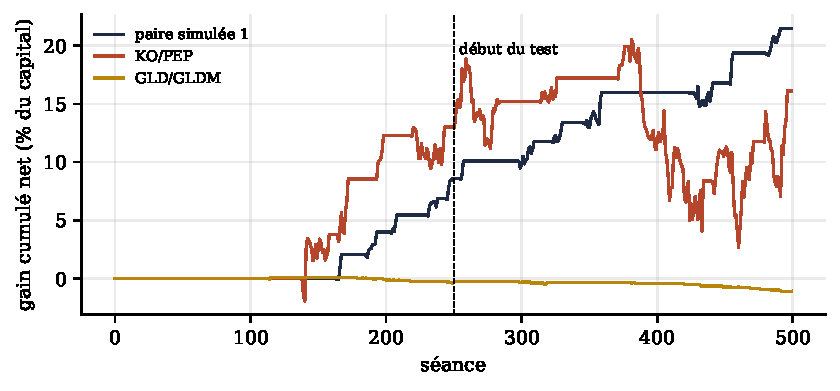
\includegraphics[width=0.85\textwidth]{ch18/go_nogo.pdf}
\caption{Gain cumulé net de la variante retenue sur la formation pour trois candidats ; la ligne pointillée sépare formation et test.}
\label{c18:fig:gonogo}
\end{figure}

\paragraph{Lecture.}
\begin{enumerate}
\item \textbf{KO/PEP} est l'exemple le plus instructif : la meilleure des 12 variantes affiche un Sharpe de 2,1 sur la formation et un gain positif sur le test (3,1\,\%). Un trader pressé déploierait. La grille dit non : la paire n'est pas cointégrée au seuil de 5\,\% et, une fois compté le nombre de variantes, le Sharpe de formation n'est pas distinguable du hasard (DSR $0{,}36$). Le Sharpe du test ($0{,}19$) le confirme a posteriori.
\item \textbf{GLD/GLDM} est parfaitement cointégrée, mais son écart revient en moins d'une séance et vaut quelques points de base : à 5 pb par jambe, aucune règle quotidienne ne couvre ses coûts (rentabilité nulle à 2,2 pb). Une relation très solide n'est pas une stratégie rentable ; elle relève, au mieux, de l'exécution intrajournalière du chapitre~15.
\item \textbf{La paire simulée 2}, pourtant réellement cointégrée, échoue au DSR sur un an de formation. La grille est volontairement conservatrice : elle rejette parfois une bonne paire. C'est le prix d'éviter d'accepter les mauvaises ; une paire rejetée de peu peut être remise en observation (\emph{paper trading} sans engagement) plutôt qu'abandonnée.
\end{enumerate}

% =====================================================================
\section{Le retard d'exécution}
% =====================================================================

Un \emph{backtest} sur clôtures suppose qu'on est exécuté au prix de clôture qui a servi à décider. En pratique, on décide après la clôture et on est exécuté plus tard : à l'ouverture suivante, ou à la clôture suivante avec un ordre au marché de clôture.

\begin{codebox}[ — E3, décider à la clôture de $t$, être exécuté à la clôture de $t+1$ (200 mondes de 1\,000 séances, 5 pb)]
\begin{center}\small
\begin{tabular}{ccccc}
\toprule
$\varphi$ & Demi-vie & Sharpe, exécution & Sharpe, exécution & Perte \\
 & & à la clôture & le lendemain & \\
\midrule
0,50 & 1,0 & 3,20 & 1,47 & $-54\,\%$ \\
0,80 & 3,1 & 2,48 & 1,93 & $-22\,\%$ \\
0,90 & 6,6 & 1,76 & 1,57 & $-11\,\%$ \\
0,95 & 13,5 & 1,15 & 1,06 & $-8\,\%$ \\
\bottomrule
\end{tabular}
\end{center}
\end{codebox}

\paragraph{Lecture.} Plus l'écart revient vite, plus un jour de retard coûte cher : avec une demi-vie d'une séance, la moitié du Sharpe disparaît. Une stratégie à demi-vie courte n'est exploitable que si l'exécution est rapide (ordres au marché de clôture, ou données et exécution intrajournalières). Le \emph{backtest} doit modéliser le délai réel d'exécution, pas le délai idéal.

% =====================================================================
\section{Surveiller le \emph{paper trading}}
% =====================================================================

\subsection{La question}

Après quelques semaines de \emph{paper trading}, la stratégie fait moins bien que son \emph{backtest}. Malchance ou \emph{backtest} trop optimiste ? On teste l'hypothèse \og le vrai Sharpe est celui du \emph{backtest}\fg{} avec la statistique
\[
Z_T = \frac{\widehat{SR}_{\text{réel},T} - SR_{\text{backtest}}}{\sqrt{1/(T-1)}},
\]
qui suit approximativement une loi normale centrée réduite sous cette hypothèse (proposition~\ref{c16:prop:sese}). On conclut à la sous-performance si $Z_T < -1{,}645$ (test unilatéral à 5\,\%).

\subsection{Le piège du contrôle quotidien}

Regarder ce test chaque jour revient à faire des centaines de tests : la probabilité de fausse alarme explose. Il faut fixer à l'avance les dates de contrôle et ajuster le seuil.

\begin{codebox}[ — E4, détection de la sous-performance en 500 jours de \emph{paper trading} (4\,000 simulations)]
\begin{center}\small
\setlength{\tabcolsep}{4pt}
\begin{tabular}{cccccc}
\toprule
Sharpe & Sharpe & Contrôle & Délai & Contrôle unique & 4 contrôles \\
vrai & annoncé & quotidien & médian & à 250 j & (Bonferroni) \\
\midrule
1,5 & 1,5 & 31,0\,\% & 56 j & 5,4\,\% & 4,0\,\% \\
1,0 & 2,0 & 67,3\,\% & 92 j & 25,1\,\% & 25,6\,\% \\
0,0 & 1,5 & 86,9\,\% & 88 j & 45,6\,\% & 52,1\,\% \\
0,0 & 3,0 & 99,9\,\% & 45 j & 91,0\,\% & 98,0\,\% \\
\bottomrule
\end{tabular}
\end{center}
Contrôle quotidien : alarme au premier jour (à partir du 20\textsuperscript{e}) où $Z_T < -1{,}645$. Quatre contrôles à 60, 125, 250 et 500 jours au seuil $\Phi^{-1}(0{,}05/4)$.
\end{codebox}

\paragraph{Lecture.} (1) Avec un contrôle quotidien, une stratégie \emph{exactement} conforme à son \emph{backtest} déclenche une fausse alarme dans 31\,\% des cas. (2) Quatre contrôles datés à l'avance, au seuil corrigé de Bonferroni, ramènent les fausses alarmes à 4\,\% tout en détectant aussi bien qu'un contrôle unique. (3) La puissance est faible : une stratégie sans aucun avantage, annoncée à Sharpe 1,5, n'est détectée que dans la moitié des cas en deux ans. Le \emph{paper trading} ne prouve pas qu'une stratégie fonctionne ; il détecte surtout les stratégies \emph{très} surestimées et les problèmes d'exécution. D'où l'importance de la grille de la section précédente, appliquée \emph{avant}.

% =====================================================================
\section{Déploiement progressif}
% =====================================================================

\begin{center}\small
\begin{tabularx}{\textwidth}{>{\raggedright}p{2.6cm}>{\raggedright}X>{\raggedright\arraybackslash}p{4.2cm}}
\toprule
Étape & Ce qu'on mesure & Condition pour passer \\
\midrule
\emph{Paper trading} (3 à 6 mois) & Parité des décisions, écart entre prix théoriques et prix qu'on aurait obtenus, incidents techniques. & Aucun incident grave ; contrôles datés non déclenchés. \\
Petite taille (1 à 3 mois) & Glissement réel, rejets, exécutions partielles, frais réels, comportement de la marge. & Coûts réels $\le$ coûts déclarés ; écart réel/\emph{backtest} expliqué. \\
Taille cible & Performance, drawdown, limites de risque. & Revue mensuelle sans dérive ; arrêt si limites atteintes. \\
\bottomrule
\end{tabularx}
\end{center}

\paragraph{Le journal.} Chaque jour : positions, ordres, prix obtenus contre prix théoriques, incidents. Chaque mois : P\&L réel contre P\&L du \emph{backtest} rejoué sur la même période (la différence est le \emph{coût d'implémentation}), état des alarmes de rupture, décisions prises et pourquoi. Le dossier \texttt{docs/specs/} conserve, pour chaque stratégie, la spécification, la décision de passage et les revues : c'est ce qui permet, six mois plus tard, de savoir si l'on a respecté son propre plan.

% =====================================================================
\section{Feuille de route pour la suite}
% =====================================================================

\begin{enumerate}
\item \textbf{Compléter le paquet} : filtre de Kalman (chapitre~8), OU et seuils optimaux (chapitre~5), copules (chapitre~9) dans \texttt{models/} ; simulateur d'exécution (chapitre~15) dans \texttt{execution/} ; chacun avec ses tests.
\item \textbf{Constituer un univers réel} : 50 à 100 ETF et actions liquides par secteur via Interactive Brokers, avec titres radiés.
\item \textbf{Première stratégie} : \emph{pairs trading} par cointégration sur ETF sectoriels, passée à la grille de ce chapitre, en \emph{paper trading}.
\item \textbf{Deuxième famille} : base et \emph{funding} (chapitre~14) sur capital propre, après étude des règles de chaque plateforme.
\item \textbf{Diversifier entre familles}, pas seulement entre paires (chapitre~17).
\end{enumerate}

% =====================================================================
\section{Ce que la théorie apporte, et ses limites}
% =====================================================================

\paragraph{Apports.} Une méthode reproductible : chaque décision (déployer, arrêter) repose sur des critères écrits à l'avance et calculés par du code testé. Les expériences montrent que cette méthode écarte des candidats séduisants (KO/PEP) et des relations solides mais inexploitables (GLD/GLDM).

\paragraph{Limites.} Les seuils de la grille (5\,\%, 30 séances, 0,95, deux fois les coûts) sont des conventions raisonnables, pas des optimums. La grille ne protège pas contre une rupture future ni contre un risque de plateforme. Enfin, aucune méthode ne transforme une absence d'avantage en avantage : elle évite seulement de croire en avoir un.

% =====================================================================
\section{Fiche à recopier au tableau blanc}
% =====================================================================

\begin{whiteboard}
\begin{itemize}[leftmargin=1.2em]
\item \textbf{Cycle :} spécification $\to$ tests $\to$ code $\to$ recherche $\to$ critères $\to$ \emph{paper} $\to$ petite taille $\to$ taille cible $\to$ revue.
\item \textbf{Parité :} version vectorisée = version événementielle, vérifiée par un test.
\item \textbf{Grille :} G0 hypothèse ; G1 $p_{EG}<0{,}05$ ; G2 demi-vie $\in[1,30]$ ; G3 DSR $>0{,}95$ ; G4 test net $>0$ ; G5 rentabilité nulle $> 2\times$ coûts.
\item \textbf{Retard :} un jour de retard coûte d'autant plus que la demi-vie est courte.
\item \textbf{Suivi :} $Z_T = (\widehat{SR}_{\text{réel}} - SR_{\text{bt}})\sqrt{T-1}$ ; contrôles datés à l'avance, seuil de Bonferroni.
\item \textbf{Journal :} coût d'implémentation = P\&L réel $-$ P\&L du \emph{backtest} rejoué.
\end{itemize}
\end{whiteboard}

% =====================================================================
\section{Exercices}
% =====================================================================

\begin{exercise}
Expliquez pourquoi la paire simulée 2 échoue au critère G3 alors qu'elle est réellement cointégrée. Combien de séances de formation faudrait-il, environ, pour que son Sharpe de formation donne un DSR supérieur à 0,95 avec 12 variantes ?
\end{exercise}

\begin{exercise}
Avec un seul contrôle à 250 jours, quelle est la probabilité de détecter une stratégie de vrai Sharpe 0 annoncée à 1,5 ? Retrouvez l'ordre de grandeur du tableau E4 par le calcul : $\E[Z_{250}] = -1{,}5\sqrt{249/252}$.
\end{exercise}

\begin{exercise}[à coder]
Remplissez \texttt{docs/specs/TEMPLATE\_strategie.md} pour une paire d'ETF sectoriels de votre choix, puis demandez à Claude Code de l'implémenter en respectant \texttt{CLAUDE.md}. Vérifiez que les tests exigés existent et passent.
\end{exercise}

\begin{exercise}[à coder]
Ajoutez à \texttt{PairStrategy} une méthode \texttt{state()} qui renvoie tout son état (fenêtres, position) et une méthode \texttt{restore()}, puis un test : un robot arrêté et redémarré au milieu de l'historique prend exactement les mêmes décisions qu'un robot jamais arrêté.
\end{exercise}

\begin{exercise}[données réelles]
Appliquez la grille de passage à cinq paires d'ETF de votre choix. Combien de variantes avez-vous essayées au total ? Combien de paires passent ?
\end{exercise}

% =====================================================================
\section{Pour aller plus loin}
% =====================================================================

\begin{toread}
\begin{itemize}[leftmargin=1.2em]
\item \citet{lopezdeprado2018}, chapitres 1 (organisation de la recherche quantitative en chaîne de production) et 11 à 13 (\emph{backtest}).
\item \citet{chan2013}, chapitre 1 (\emph{backtesting} et exécution automatisée) : les écarts courants entre \emph{backtest} et réel.
\item \citet{beck2002} : le développement piloté par les tests, la méthode utilisée dans le dépôt.
\item Le dépôt \texttt{atjte} \citep{atjte}, dossier \texttt{tests/} : un exemple de suite de tests d'un moteur d'exécution réel.
\item Chapitre~0 de ce cours, section sur l'architecture du dépôt, et le fichier \texttt{CLAUDE.md}.
\end{itemize}
\end{toread}

\section{Scripts du chapitre}
\sloppy\noindent\texttt{code/ch18/ch18\_pipeline.py} : E1, E2 (figure~\ref{c18:fig:gonogo}), E3, E4.\par\noindent Modules : \texttt{src/arbhub/signals/pair\_strategy.py}, \texttt{src/arbhub/data/loaders.py}.\par\noindent Tests : \texttt{tests/test\_pair\_strategy.py}.


\appendix
% =====================================================================
%  Annexes
% =====================================================================

\chapter{Formulaire récapitulatif}
\label{ann:formulaire}

Cette annexe rassemble les fiches \og tableau blanc\fg{} de tous les chapitres. Elle est générée automatiquement par \texttt{docs/cours/make\_formulaire.py}.

\section*{Chapitre 1 — Arbitrage, stationnarité et retour à la moyenne}
\addcontentsline{toc}{section}{Chapitre 1 — Arbitrage, stationnarité et retour à la moyenne}
\begin{itemize}[leftmargin=1.2em,itemsep=0.05em]
\item \textbf{Arbitrage pur :} coût $\le 0$, perte impossible, gain possible. \textbf{Statistique :} $v(0)=0$, $\E[v(t)]\to>0$, $\Prob(v(t)<0)\to0$, $\Var(v(t))/t\to0$.
\item \textbf{Variance d'un écart :} $\Var(Y-\beta X) = \sigma_Y^2 + \beta^2\sigma_X^2 - 2\beta\Cov(X,Y)$.
\item \textbf{Couverture optimale :} $\beta^\star = \Cov(X,Y)/\sigma_X^2 = \rho\,\sigma_Y/\sigma_X$ ; variance restante $\sigma_Y^2(1-\rho^2)$.
\item \textbf{Stationnarité faible :} $\E X_t = \mu$, $\Var X_t = \gamma(0)$, $\Cov(X_t,X_{t-h}) = \gamma(h)$, indépendants de $t$.
\item \textbf{Marche aléatoire :} $P_t = P_0 + \sum\varepsilon_i$ ; $\E P_t = P_0$ ; $\Var P_t = t\sigma^2$ ; non stationnaire ; $I(1)$.
\item \textbf{AR(1) :} $X_t - \mu = \varphi(X_{t-1}-\mu) + \varepsilon_t$ ; stationnaire si $|\varphi|<1$ ; $\mu = c/(1-\varphi)$ ; $\gamma(0) = \sigma^2/(1-\varphi^2)$ ; $\rho(h) = \varphi^h$.
\item \textbf{Retour à la moyenne :} $\Delta X_t = -(1-\varphi)(X_{t-1}-\mu) + \varepsilon_t$.
\item \textbf{Demi-vie :} $h_{1/2} = -\ln2/\ln\varphi \approx \ln 2/(1-\varphi)$.
\item \textbf{Cointégration (intuition) :} $X, Y \sim I(1)$ et $Y - \beta X \sim I(0)$.
\item \textbf{Z-score :} $z_t = (S_t - m)/d$, avec $m$, $d$ estimés \emph{sur la formation seulement}.
\item \textbf{Gain sans anticipation :} $G_{t+1} = q_t(S_{t+1}-S_t)$.
\end{itemize}

\section*{Chapitre 2 — Régression et estimation}
\addcontentsline{toc}{section}{Chapitre 2 — Régression et estimation}
\begin{itemize}[leftmargin=1.2em,itemsep=0.05em]
\item \textbf{MCO simples :} $\hat b = \sum(x-\bar x)(y-\bar y)/\sum(x-\bar x)^2$, $\hat a = \bar y - \hat b\bar x$.
\item \textbf{MCO matriciels :} $\hat\beta = (X^\top X)^{-1}X^\top y$ ; $X^\top e = 0$ ; $\hat\sigma^2 = e^\top e/(n-k)$.
\item \textbf{Sans biais :} $\hat\beta = \beta + (X^\top X)^{-1}X^\top\varepsilon$ ; $\Var(\hat\beta) = \sigma^2(X^\top X)^{-1}$ sous (H4).
\item \textbf{Sandwich :} $(X^\top X)^{-1}\,\hat\Omega\,(X^\top X)^{-1}$ ; Newey-West : poids $1-j/(L+1)$.
\item \textbf{Asymétrie :} $\hat\beta_{Y|X}\hat\beta_{X|Y} = \hat\rho^2$.
\item \textbf{Orthogonale :} $s_{XY}b^2 + (s_{XX}-s_{YY})b - s_{XY} = 0$, racine de même signe que $s_{XY}$.
\item \textbf{Log-vraisemblance AR(1) :} $\ell = -\frac n2\ln(2\pi\sigma^2) - \frac1{2\sigma^2}\sum(x_t - c - \varphi x_{t-1})^2$ ; MV conditionnel $=$ MCO.
\item \textbf{Asymptotique :} $\Var(\hat\varphi)\approx(1-\varphi^2)/n$.
\item \textbf{Correction de Kendall :} $\hat\varphi_c = \hat\varphi + (1+3\hat\varphi)/n$.
\end{itemize}

\section*{Chapitre 3 — Tester la stationnarité et le retour à la moyenne}
\addcontentsline{toc}{section}{Chapitre 3 — Tester la stationnarité et le retour à la moyenne}
\begin{itemize}[leftmargin=1.2em,itemsep=0.05em]
\item \textbf{DF :} $\Delta x_t = c + \gamma x_{t-1} + \varepsilon_t$, $H_0 : \gamma = 0$ (racine unitaire), $\tau = \hat\gamma/\mathrm{se}$.
\item \textbf{Pourquoi non normale :} $\sum x_{t-1}\varepsilon_t = \frac12(x_n^2 - \sum\varepsilon_t^2)$ $\Rightarrow$ $\frac12(W^2-1)$, négatif 68\,\% du temps.
\item \textbf{Seuils 5\,\% :} $-1{,}95$ (rien), $-2{,}86$ (constante), $-3{,}41$ (tendance).
\item \textbf{ADF :} ajouter $\sum\delta_j\Delta x_{t-j}$, choisir $p$ par AIC.
\item \textbf{Puissance :} gouvernée par $n(1-\varphi)\approx 0{,}69\,n/h_{1/2}$ ; viser $\ge 30$ demi-vies.
\item \textbf{KPSS :} $H_0$ stationnarité ; $\eta = n^{-2}\sum S_t^2/\hat\sigma^2_{LR}$ ; seuil $0{,}463$.
\item \textbf{Ratio de variance :} $VR(q) = \Var(x_{t+q}-x_t)/(q\Var(\Delta x))$ ; AR(1) : $(1-\varphi^q)/(q(1-\varphi))$.
\item \textbf{Hurst :} $\mathrm{sd}(x_{t+\tau}-x_t)\propto\tau^H$ ; $H<\frac12$ retour, $=\frac12$ marche, $>\frac12$ tendance.
\end{itemize}

\section*{Chapitre 4 — Cointégration}
\addcontentsline{toc}{section}{Chapitre 4 — Cointégration}
\begin{itemize}[leftmargin=1.2em,itemsep=0.05em]
\item \textbf{$I(d)$ :} différencier $d$ fois pour être stationnaire. Prix $\sim I(1)$.
\item \textbf{Cointégration :} $x\sim I(1)$, $\beta^\top x\sim I(0)$ ; rang $r$ = nombre de relations indépendantes.
\item \textbf{Engle-Granger :} MCO en niveaux, puis ADF sur résidus ; seuils 5\,\% : $-3{,}34$ (2 var.), $-3{,}74$ (3 var.).
\item \textbf{Superconvergence :} $\hat b - b = O(1/n)$ si la paire est cointégrée.
\item \textbf{Correction d'erreur :} $\Delta x_{1t} = \alpha_1S_{t-1}+\dots$, $\Delta x_{2t} = \alpha_2S_{t-1}+\dots$ ; $\varphi_S = 1+\alpha_1-\beta\alpha_2$.
\item \textbf{VECM :} $\Delta x_t = \Pi x_{t-1} + \sum\Gamma_i\Delta x_{t-i} + \varepsilon_t$, $\Pi = \alpha\beta^\top$, rang $r$.
\item \textbf{Johansen :} trace $= -T\sum_{i>r}\ln(1-\hat\lambda_i)$ ; tester $r = 0, 1, \dots$
\item \textbf{Cointégration partielle :} $S = M + R$ ; $R^2_{MR} = 2\sigma_M^2/(2\sigma_M^2 + (1+\rho)\sigma_R^2)$.
\end{itemize}

\section*{Chapitre 5 — Le processus d'Ornstein-Uhlenbeck}
\addcontentsline{toc}{section}{Chapitre 5 — Le processus d'Ornstein-Uhlenbeck}
\begin{itemize}[leftmargin=1.2em,itemsep=0.05em]
\item \textbf{Brownien :} $W_t - W_s\sim\N(0,t-s)$, $(\dd W)^2 = \dd t$.
\item \textbf{Itô :} $\dd f = (\partial_tf + b\,\partial_xf + \frac12s^2\partial_{xx}f)\dd t + s\,\partial_xf\,\dd W$.
\item \textbf{OU :} $\dd X = \theta(\mu - X)\dd t + \sigma\dd W$ ; $X_t = \mu + (X_0-\mu)e^{-\theta t} + \sigma\int_0^te^{-\theta(t-u)}\dd W_u$.
\item \textbf{Moments :} moyenne $\mu + (X_0-\mu)e^{-\theta t}$ ; variance $\frac{\sigma^2}{2\theta}(1-e^{-2\theta t})$ ; $\sigma_{eq} = \sigma/\sqrt{2\theta}$ ; $h_{1/2} = \ln2/\theta$.
\item \textbf{OU $\leftrightarrow$ AR(1) :} $\varphi = e^{-\theta\Delta}$, $\sigma_\eta^2 = \frac{\sigma^2}{2\theta}(1-\varphi^2)$ ; $\hat\theta = -\ln\hat\varphi/\Delta$.
\item \textbf{Kolmogorov :} $\frac12s^2u'' + bu' = -1$.
\item \textbf{Retour :} $T_{a\to0} = \frac2{\sigma^2}\int_0^ae^{ky^2}\int_y^\infty e^{-kz^2}\dd z\,\dd y$, $k=\theta/\sigma^2$.
\item \textbf{Seuil optimal :} maximiser $(a-c)/(T_{0\to\pm a}+T_{a\to0})$ ; le seuil monte avec les coûts.
\end{itemize}

\section*{Chapitre 6 — La méthode des distances}
\addcontentsline{toc}{section}{Chapitre 6 — La méthode des distances}
\begin{itemize}[leftmargin=1.2em,itemsep=0.05em]
\item \textbf{Formation 12 mois :} $\tilde P_{i,t} = P_{i,t}/P_{i,0}$, $\mathrm{SSD}_{ij} = \sum_t(\tilde P_{i,t}-\tilde P_{j,t})^2$, top 20 paires.
\item \textbf{Calcul matriciel :} $\mathrm{SSD} = \mathrm{diag}(G)\mathbf 1^\top + \mathbf 1\mathrm{diag}(G)^\top - 2G$, $G = \tilde P^\top\tilde P$.
\item \textbf{Trading 6 mois :} ouvrir à $|D_t| > 2\hat\sigma$ (1\,\$ long / 1\,\$ court), fermer au croisement.
\item \textbf{Gain d'un trade :} $(P^L_{t_1}/P^L_{t_0}-1) - (P^C_{t_1}/P^C_{t_0}-1)$.
\item \textbf{Capital engagé :} somme des gains / 20 ; \textbf{employé :} / nombre de paires ouvertes.
\item \textbf{Biais de la SSD :} $\mathrm{SSD}/T = \bar D^2 + \widehat\Var(D)$ : favorise les écarts peu volatils.
\end{itemize}

\section*{Chapitre 7 — Cointégration appliquée : sélectionner les paires sans se mentir}
\addcontentsline{toc}{section}{Chapitre 7 — Cointégration appliquée : sélectionner les paires sans se mentir}
\begin{itemize}[leftmargin=1.2em,itemsep=0.05em]
\item \textbf{Faux positifs attendus :} $m\alpha$, avec $m = N(N-1)/2$.
\item \textbf{FWER} $=\Prob(V\ge1)$ ; \textbf{FDR} $=\E[V/\max(R,1)]$.
\item \textbf{Bonferroni :} rejeter si $p < \alpha/m$ ; preuve par l'inégalité de la réunion.
\item \textbf{BH :} plus grand $k$ tel que $p_{(k)}\le kq/m$ ; rejeter les $k$ plus petites.
\item \textbf{Pipeline :} a priori économique $\to$ test corrigé $\to$ demi-vie et amplitude $\to$ stabilité $\to$ contraintes pratiques.
\item \textbf{Erreur-type honnête :} regrouper par univers ou période, jamais par paire si les paires partagent des actifs.
\item \textbf{Taille :} notionnel $K = R/\sigma_S$.
\end{itemize}

\section*{Chapitre 8 — Modèles espace-état et filtre de Kalman}
\addcontentsline{toc}{section}{Chapitre 8 — Modèles espace-état et filtre de Kalman}
\begin{itemize}[leftmargin=1.2em,itemsep=0.05em]
\item \textbf{Modèle :} $\xi_t = F\xi_{t-1} + w_t$ ($Q$) ; $y_t = H_t\xi_t + v_t$ ($R$).
\item \textbf{Conditionnement :} $\E[X|y] = \mu_X + \Sigma_{XY}\Sigma_{YY}^{-1}(y-\mu_Y)$ ; $\Var = \Sigma_{XX} - \Sigma_{XY}\Sigma_{YY}^{-1}\Sigma_{YX}$.
\item \textbf{Prédiction :} $m^- = Fm$, $P^- = FPF^\top + Q$.
\item \textbf{Innovation :} $e = y - Hm^-$, $F_t = HP^-H^\top + R$.
\item \textbf{Mise à jour :} $K = P^-H^\top F_t^{-1}$, $m = m^- + Ke$, $P = P^- - KHP^-$.
\item \textbf{Scalaire :} $K = P/(P+R)$.
\item \textbf{Vraisemblance :} $\ell = -\frac12\sum(\ln 2\pi F_t + e_t^2/F_t)$.
\item \textbf{Ratio variable :} $\xi = (\alpha,\beta)$, $F = I$, $Q = \frac\delta{1-\delta}I$, $H_t = (1,x_t)$ ; signal $e_t/\sqrt{F_t}$.
\end{itemize}

\section*{Chapitre 9 — Copules}
\addcontentsline{toc}{section}{Chapitre 9 — Copules}
\begin{itemize}[leftmargin=1.2em,itemsep=0.05em]
\item \textbf{Transformation :} $U = F_X(X)\sim\mathcal U[0,1]$.
\item \textbf{Sklar :} $H(x,y) = C(F_X(x),F_Y(y))$.
\item \textbf{Kendall :} $\tau = \Prob(\text{concordance}) - \Prob(\text{discordance})$ ; gaussienne/Student : $\rho = \sin(\pi\tau/2)$ ; Clayton : $\theta = 2\tau/(1-\tau)$.
\item \textbf{Queue :} $\lambda_L = \lim_{q\to0}\Prob(V\le q\mid U\le q)$ ; Clayton $2^{-1/\theta}$ ; gaussienne 0.
\item \textbf{Clayton :} $C = (u^{-\theta}+v^{-\theta}-1)^{-1/\theta}$.
\item \textbf{Fonction $h$ :} $h(u|v) = \partial C/\partial v$ ; gaussienne $\Phi\big((\Phi^{-1}(u)-\rho\Phi^{-1}(v))/\sqrt{1-\rho^2}\big)$.
\item \textbf{Pseudo-observations :} rang$/(n+1)$ ; choix par AIC $= 2k-2\ell$.
\end{itemize}

\section*{Chapitre 10 — Arbitrage statistique multi-actifs}
\addcontentsline{toc}{section}{Chapitre 10 — Arbitrage statistique multi-actifs}
\begin{itemize}[leftmargin=1.2em,itemsep=0.05em]
\item \textbf{ACP :} $\max_w w^\top Cw$ s.c. $w^\top w=1$ $\Rightarrow$ $Cw = \lambda w$ ; part expliquée $\sum_{j\le k}\lambda_j/N$.
\item \textbf{Portefeuille propre :} $Q_{ij} = v_{j,i}/\sigma_i$, $F_{jt} = \sum_iQ_{ij}R_{it}$.
\item \textbf{Marchenko-Pastur :} bruit entre $(1\pm\sqrt{N/T})^2$.
\item \textbf{Modèle :} $R_i = \alpha_i + \sum_j\beta_{ij}F_j + \dd X_i$, $X_i$ OU.
\item \textbf{AR(1) sur $X$ :} $\kappa = -252\ln b$, $m = a/(1-b)$, $\sigma_{eq} = \sqrt{\Var(\zeta)/(1-b^2)}$.
\item \textbf{s-score :} $s = (X - m)/\sigma_{eq}$ ; ouvrir à $\pm1{,}25$, fermer court à $0{,}75$, long à $-0{,}5$ ; filtre $\kappa > 252/30$.
\item \textbf{Box-Tiao :} minimiser $w^\top A\Gamma A^\top w/w^\top\Gamma w$.
\end{itemize}

\section*{Chapitre 11 — Apprentissage automatique}
\addcontentsline{toc}{section}{Chapitre 11 — Apprentissage automatique}
\begin{itemize}[leftmargin=1.2em,itemsep=0.05em]
\item \textbf{Variable :} calculable en $t$ ; \textbf{étiquette :} regarde vers $t+H$.
\item \textbf{Chevauchement :} étiquettes à horizon $H$ partagent $H-1$ jours $\Rightarrow$ K-fold mélangé fuit.
\item \textbf{Remède :} walk-forward, purge des dates qui chevauchent le test, embargo.
\item \textbf{Test de base :} toujours comparer à une règle simple sur le même échantillon de test.
\item \textbf{Sélection :} ACP (expositions) $\to$ OPTICS (groupes) $\to$ cointégration intra-groupe $+$ BH.
\end{itemize}

\section*{Chapitre 12 — Microstructure et coûts de transaction}
\addcontentsline{toc}{section}{Chapitre 12 — Microstructure et coûts de transaction}
\begin{itemize}[leftmargin=1.2em,itemsep=0.05em]
\item \textbf{Fourchette :} ask $-$ bid ; mid $=$ (bid+ask)/2 ; taker paie la demi-fourchette, maker la reçoit mais subit la sélection adverse.
\item \textbf{Roll :} $\Cov(\Delta p_t,\Delta p_{t-1}) = -s^2/4$ $\Rightarrow$ $s = 2\sqrt{-\Cov}$ (données de transaction seulement).
\item \textbf{Aller-retour de paire :} $4c$ + emprunt.
\item \textbf{Règle :} $\sigma_{eq}\ge$ coût d'un aller-retour.
\item \textbf{Impact :} $Y\sigma_{\text{jour}}\sqrt{Q/V}$.
\item \textbf{Backtest :} exécuter au plus tôt en $t+1$ ; payer la demi-fourchette.
\end{itemize}

\section*{Chapitre 13 — Arbitrage spatial et triangulaire}
\addcontentsline{toc}{section}{Chapitre 13 — Arbitrage spatial et triangulaire}
\begin{itemize}[leftmargin=1.2em,itemsep=0.05em]
\item \textbf{Spatial :} opportunité si $b_B/a_A > (1+f_A)/(1-f_B)\approx1+f_A+f_B$.
\item \textbf{Inventaire :} rééquilibrage rentable si $Q > 10^4K/e$ ($K$ coût de transfert, $e$ avantage en pb).
\item \textbf{Écart persistant :} chercher la friction (contrôle des capitaux, transfert, contrepartie).
\item \textbf{Latence :} le premier prend tout ; durée de vie en millisecondes $\Rightarrow$ inaccessible au particulier.
\item \textbf{Triangulaire :} profitable si $z^{bid}(1-f)^3/(x^{ask}y^{ask}) > 1$ ; probabilité $2\Prob(Z > 3(h+f)/(\sigma_n\sqrt3))$.
\item \textbf{Ligne rouge :} arbitrage de latence contre un courtier ou une \emph{prop firm} : interdit.
\end{itemize}

\section*{Chapitre 14 — Arbitrage de base, \emph{cash-and-carry} et \emph{funding}}
\addcontentsline{toc}{section}{Chapitre 14 — Arbitrage de base, \emph{cash-and-carry} et \emph{funding}}
\begin{itemize}[leftmargin=1.2em,itemsep=0.05em]
\item \textbf{Portage :} $F = Se^{(r-q)T}$ ; base $F - S\to0$ à l'échéance.
\item \textbf{Bande :} $Se^{(r_l-q)T} - c' \le F \le Se^{(r_b-q)T} + c$.
\item \textbf{Cash-and-carry :} long comptant financé, court future ; gain final fixé, besoin de marge variable.
\item \textbf{Funding :} longs paient les courts si perpétuel $>$ indice ; formule propre à chaque plateforme.
\item \textbf{Liquidation :} hausse de $\approx 1/L - m$ sur la jambe courte.
\item \textbf{atjte :} $s_t = P^{\text{plat}} - kP^{\text{MT5}}$ ; maker sur la plateforme, taker sur MT5 ; centre théorique $=$ référence $\times$ portage $\times$ jours$/365$.
\end{itemize}

\section*{Chapitre 15 — Exécution, couverture et architecture logicielle}
\addcontentsline{toc}{section}{Chapitre 15 — Exécution, couverture et architecture logicielle}
\begin{itemize}[leftmargin=1.2em,itemsep=0.05em]
\item \textbf{Risque de jambe :} écart-type $\sigma\sqrt\Delta$ ; nul en espérance seulement si le délai est indépendant des prix.
\item \textbf{Sélection adverse :} un ordre maker est exécuté quand le marché lui donne tort ; coût croissant avec le retard de recotation.
\item \textbf{Où coter :} sur la plateforme suiveuse ; couvrir sur la meneuse.
\item \textbf{Architecture :} passerelles, contrôle du ratio, lot minimal, réconciliation sur positions réelles, sommeil si flux périmé, un robot par contrat, mode simulation, journaux.
\end{itemize}

\section*{Chapitre 16 — \emph{Backtest} rigoureux}
\addcontentsline{toc}{section}{Chapitre 16 — \emph{Backtest} rigoureux}
\begin{itemize}[leftmargin=1.2em,itemsep=0.05em]
\item \textbf{Sans anticipation :} $\text{gain}_{t+1} = q_t(S_{t+1}-S_t)$, $q_t$ fonction des seules données $\le t$ ; test automatique : modifier le futur ne change pas le passé.
\item \textbf{Trois biais :} anticipation, survie (garder les radiés), sélection (compter les essais).
\item \textbf{Erreur-type du Sharpe :} $\sqrt{(1+SR^2/2)/T}$ par période ; annualisé $\approx 1/\sqrt{\text{années}}$.
\item \textbf{Maximum de $N$ Sharpe nuls :} $\approx\sqrt V\big((1-\gamma)\Phi^{-1}(1-\tfrac1N) + \gamma\Phi^{-1}(1-\tfrac{1}{Ne})\big)$, croît comme $\sqrt{2\ln N/T}$.
\item \textbf{PSR :} $\Phi\big((\widehat{SR}-SR^\ast)\sqrt{T-1}/\sqrt{1-\gamma_3\widehat{SR}+\frac{\gamma_4-1}{4}\widehat{SR}^2}\big)$ ; \textbf{DSR :} PSR avec $SR^\ast = \E[\max]$.
\item \textbf{PBO :} proportion des découpages CSCV où la meilleure variante en sélection finit sous la médiane en test.
\item \textbf{Découpage :} formation, validation, test regardé une seule fois ; \emph{walk-forward} ; purge et embargo.
\end{itemize}

\section*{Chapitre 17 — Risque et limites de l'arbitrage}
\addcontentsline{toc}{section}{Chapitre 17 — Risque et limites de l'arbitrage}
\begin{itemize}[leftmargin=1.2em,itemsep=0.05em]
\item \textbf{Kelly :} $g(f) \approx f\mu - \tfrac12 f^2\sigma^2$ ; $f^\star = \mu/\sigma^2$ ; $g(f^\star) = SR^2/2$ ; $g(2f^\star) = 0$ ; en pratique $0{,}1$ à $0{,}25\,f^\star$.
\item \textbf{Ciblage de volatilité :} $w_t = \min(\sigma^\ast/\hat\sigma_t, L_{\max})$, $\hat\sigma_t$ estimée sur le passé.
\item \textbf{Protections :} stop $|z|>4$ (quasi gratuit) ; durée $> 3$ demi-vies ; CUSUM $S^\pm_t = \max(0, S^\pm_{t-1} \pm z_t - k)$, alarme si $> h$.
\item \textbf{Limites de l'arbitrage :} perte latente $\Rightarrow$ appel de marge $\Rightarrow$ liquidation au pire moment ; levier choisi sur le pire élargissement.
\item \textbf{Diversification :} $\sigma_P = \sigma\sqrt{1/N + \rho(1-1/N)}$ ; $N_{\text{eff}} = N/(1+(N-1)\rho)$ ; $\rho$ monte en crise.
\item \textbf{Hors statistique :} plateforme, contrepartie, courtier, emprunt de titres, opérations sur titres, réglementation, \emph{prop firms}, erreurs opérationnelles.
\end{itemize}

\section*{Chapitre 18 — Du papier au code avec Claude Code}
\addcontentsline{toc}{section}{Chapitre 18 — Du papier au code avec Claude Code}
\begin{itemize}[leftmargin=1.2em,itemsep=0.05em]
\item \textbf{Cycle :} spécification $\to$ tests $\to$ code $\to$ recherche $\to$ critères $\to$ \emph{paper} $\to$ petite taille $\to$ taille cible $\to$ revue.
\item \textbf{Parité :} version vectorisée = version événementielle, vérifiée par un test.
\item \textbf{Grille :} G0 hypothèse ; G1 $p_{EG}<0{,}05$ ; G2 demi-vie $\in[1,30]$ ; G3 DSR $>0{,}95$ ; G4 test net $>0$ ; G5 rentabilité nulle $> 2\times$ coûts.
\item \textbf{Retard :} un jour de retard coûte d'autant plus que la demi-vie est courte.
\item \textbf{Suivi :} $Z_T = (\widehat{SR}_{\text{réel}} - SR_{\text{bt}})\sqrt{T-1}$ ; contrôles datés à l'avance, seuil de Bonferroni.
\item \textbf{Journal :} coût d'implémentation = P\&L réel $-$ P\&L du \emph{backtest} rejoué.
\end{itemize}


% =====================================================================
\chapter{Notations}
\label{ann:notations}
% =====================================================================

\begin{center}\small
\begin{longtable}{>{\raggedright}p{3.2cm}>{\raggedright\arraybackslash}p{10.6cm}}
\toprule
Symbole & Signification \\
\midrule
\endhead
$t$, $T$, $n$ & date (en périodes), nombre total de périodes, taille d'échantillon \\
$X_t$, $Y_t$ ou $x_t$, $y_t$ & prix (ou log-prix) des deux jambes d'une paire \\
$S_t$, $s_t$ & écart (\emph{spread}) : $S_t = Y_t - \beta X_t$ (ou en log-prix) \\
$\beta$, $\hat\beta$ & ratio de couverture, et son estimation \\
$\varepsilon_t$, $\eta_t$ & bruit blanc (chocs non corrélés, moyenne nulle) \\
$\mu$, $\sigma$, $\sigma^2$ & moyenne, écart-type, variance \\
$\rho$, $\rho(h)$ & corrélation ; autocorrélation au retard $h$ \\
$\gamma(h)$ & autocovariance au retard $h$ \\
$\varphi$ & coefficient autorégressif de l'AR(1) \\
$h_{1/2}$ & demi-vie : $-\ln2/\ln\varphi$ (discret), $\ln2/\theta$ (continu) \\
$\theta$, $\sigma_{eq}$ & vitesse de retour et écart-type d'équilibre d'un processus d'Ornstein-Uhlenbeck \\
$W_t$ & mouvement brownien standard \\
$I(d)$ & intégré d'ordre $d$ (stationnaire après $d$ différenciations) \\
$\Delta x_t$ & différence première $x_t - x_{t-1}$ \\
$z_t$ & \emph{z-score} : $(S_t - m)/d$ avec $m$, $d$ estimés sur le passé \\
$q_t$ & position décidée à la clôture de $t$ (en unités d'écart), appliquée de $t$ à $t+1$ \\
$c$, pb & coût par jambe ; point de base $=10^{-4}$ \\
$\Phi$, $\Phi^{-1}$ & fonction de répartition et quantile de la loi normale centrée réduite \\
$SR$, $\widehat{SR}$ & ratio de Sharpe (par période ou annualisé, précisé à chaque usage) \\
PSR, DSR, PBO & Sharpe probabiliste, Sharpe déflaté, probabilité de surapprentissage \\
$f^\star$ & levier de Kelly $\mu/\sigma^2$ \\
$F$, $S$, $r$, $q$ & prix à terme, prix comptant, taux sans risque, rendement de détention (chapitre~14) \\
$\N(\mu,\sigma^2)$, $\iid$ & loi normale ; indépendantes et identiquement distribuées \\
\bottomrule
\end{longtable}
\end{center}

% =====================================================================
\chapter{Glossaire}
\label{ann:glossaire}
% =====================================================================

\begin{description}[leftmargin=0pt,itemsep=0.3em]
\item[Arbitrage pur.] Stratégie sans coût initial, sans possibilité de perte, avec une possibilité de gain (chapitre~1).
\item[Arbitrage statistique.] Stratégie sans coût initial dont le gain espéré est positif et dont la probabilité de perte tend vers zéro à long terme (chapitre~1).
\item[Base.] Écart entre le prix à terme et le prix comptant d'un même sous-jacent (chapitre~14).
\item[\emph{Cash-and-carry}.] Achat du comptant financé et vente du contrat à terme, pour capter la base (chapitre~14).
\item[Cointégration.] Relation entre séries $I(1)$ dont une combinaison linéaire est stationnaire (chapitre~4).
\item[Copule.] Fonction qui décrit la dépendance entre variables indépendamment de leurs lois marginales (chapitre~9).
\item[CUSUM.] Somme cumulée des écarts standardisés, utilisée pour détecter un changement de régime (chapitre~17).
\item[Demi-vie.] Durée au bout de laquelle l'écart espéré à la moyenne est divisé par deux (chapitres~1 et~5).
\item[\emph{Drawdown}.] Perte depuis le plus haut historique de la courbe de gains.
\item[\emph{Funding}.] Paiement périodique entre acheteurs et vendeurs d'un contrat perpétuel, qui ramène son prix vers l'indice (chapitre~14).
\item[Jambe.] Chacun des instruments d'une position d'arbitrage. \emph{Risque de jambe} : une jambe exécutée, l'autre non ou en retard (chapitre~15).
\item[\emph{Maker}, \emph{taker}.] Ordre qui apporte de la liquidité au carnet (limite, en attente), ordre qui en prend (exécuté immédiatement) (chapitre~12).
\item[\emph{Paper trading}.] Exécution simulée en temps réel, sans argent engagé (chapitre~18).
\item[Parité.] Égalité des décisions entre la version de recherche et la version de production d'une stratégie (chapitre~18).
\item[Point de base (pb).] Un centième de pourcent : $10^{-4}$.
\item[\emph{Prop firm}.] Société qui finance des traders sous conditions ; ses règles interdisent en général l'arbitrage de latence et la couverture croisée entre comptes.
\item[Régression fallacieuse.] Relation apparente entre séries non stationnaires indépendantes (chapitre~1).
\item[Sélection adverse.] Tendance d'un ordre \emph{maker} à être exécuté précisément quand le marché lui donne tort (chapitre~15).
\item[Stationnarité.] Moyenne, variance et autocovariances constantes dans le temps (chapitre~1).
\item[Surapprentissage.] Choix de paramètres qui décrivent le bruit de l'échantillon plutôt qu'une régularité durable (chapitre~16).
\item[\emph{Walk-forward}.] Validation glissante : estimer sur le passé, trader sur la période suivante, avancer (chapitre~16).
\item[\emph{Z-score}.] Écart standardisé $(S_t - m)/d$ (chapitre~1).
\end{description}

% =====================================================================
\chapter{Reproduire les résultats du cours}
\label{ann:repro}
% =====================================================================

\section*{Installation}
\begin{lstlisting}[language=bash]
git clone https://github.com/OptiWealthSolutions/arbitrage_hub.git
cd arbitrage_hub
python -m venv .venv && source .venv/bin/activate
pip install -r requirements.txt
pytest -q                                   # 24 tests
\end{lstlisting}

\section*{Scripts par chapitre}

Chaque chiffre du cours provient d'un script à graine fixée ; relancer le script redonne exactement les mêmes nombres. Les résultats sont écrits dans \texttt{code/chXX/results.json} (\texttt{code/ch01/results/} pour le chapitre~1) et les figures dans \texttt{docs/cours/figures/chXX/}.

\begin{center}\small
\begin{longtable}{>{\raggedright}p{1.1cm}>{\ttfamily\footnotesize}p{6.4cm}>{\raggedright\arraybackslash}p{6.0cm}}
\toprule
Ch. & \normalfont Script & Contenu \\
\midrule
\endhead
1 & ch01/h1 à h5\_*.py & marche aléatoire, AR(1) et demi-vie, corrélation contre cointégration, régression fallacieuse, règle en \emph{z-score} \\
2 & ch02/ch02\_regression.py & MCO, asymétrie, régression orthogonale, vraisemblance AR(1), biais \\
3 & ch03/ch03\_stationarity\_tests.py & Dickey-Fuller, puissance, KPSS, ratio de variance, Hurst, cas réels \\
4 & ch04/ch04\_cointegration.py & Engle-Granger, correction d'erreur, Johansen, cointégration partielle \\
5 & ch05/ch05\_ornstein\_uhlenbeck.py & simulation exacte, estimation, temps de passage, seuils optimaux \\
6 & ch06/ch06\_distance\_method.py & méthode des distances (Gatev et al.) \\
7 & ch07/ch07\_cointegration\_selection.py & sélection de paires, faux positifs, Bonferroni, BH \\
8 & ch08/ch08\_kalman.py & filtre de Kalman, ratio variable \\
9 & ch09/ch09\_copulas.py & copules, fonction $h$, cas KO/PEP \\
10 & ch10/ch10\_pca\_statarb.py & ACP, Marchenko-Pastur, \emph{s-score} \\
11 & ch11/ch11\_machine\_learning.py & fuite d'information, validation purgée, sélection par \emph{clustering} \\
12 & ch12/ch12\_microstructure.py & fourchette, Roll, impact, coûts d'un aller-retour \\
13 & ch13/ch13\_spatial\_triangular.py & arbitrage spatial, triangulaire, course de latence \\
14 & ch14/ch14\_basis\_funding.py & portage, \emph{cash-and-carry}, \emph{funding}, liquidation \\
15 & ch15/ch15\_execution.py & risque de jambe, sélection adverse \\
16 & ch16/ch16\_backtest.py & biais d'anticipation, Sharpe, DSR, PBO, survie \\
17 & ch17/ch17\_risk.py & Kelly, protections contre la rupture, spirale de marge, diversification \\
18 & ch18/ch18\_pipeline.py & parité, critères de passage, retard d'exécution, suivi du \emph{paper trading} \\
\bottomrule
\end{longtable}
\end{center}

\section*{Recompiler ce document}
\begin{lstlisting}[language=bash]
cd docs/cours && sh build.sh     # formulaire regénéré, 3 passes LaTeX + BibTeX
\end{lstlisting}

\section*{Données réelles}
Les études de cas utilisent 500 clôtures quotidiennes de GLD, GLDM, KO et PEP (21 octobre 2024 au 19 octobre 2026) téléchargées via Interactive Brokers ; voir \texttt{data/case\_studies/README.md}. Prix non ajustés des dividendes.

\section*{Avertissement}
Ce cours est un support pédagogique et non un conseil en investissement. Les performances citées, qu'elles proviennent de la littérature ou des simulations, ne préjugent pas des performances futures. Vérifiez les conditions de vos courtiers et plateformes avant tout déploiement ; les stratégies d'arbitrage inter-plateformes ne doivent pas être utilisées sur des comptes de \emph{prop firms}.


\bibliographystyle{plainnat}
\bibliography{references}

\end{document}
